% ---------------------------------------------------------------------------------------------------------------
% TEMPLATE PARA TRABALHO DE CONCLUSÃO DE CURSO
% Universidade Tecnológica Federal do Paraná - UTFPR
% Customização da classe abnTeX2 (http://www.abntex.net.br/) para as normas da UTFPR
%
% Autores: Diego Marczal
% 	       Michael Vornes <https://github.com/mvornes>
% Adaptação (DACOM-CP): Silvio Ricardo Rodrigues Sanches
%
%----------------------------------------------------------------------------------------------------------------
% Codificação: UTF-8
% LaTeX:  abnTeX2          
% ---------------------------------------------------------------------------------------------------------------


% CARREGA CLASSE PERSONALIZADA DA UTFPR--------------------------------------------------------------------------
\documentclass[%twoside,                   % Impressão em frente e verso
    	        oneside,                   % Impressão apenas frente
]{configuracoes/utfpr-abntex2}


% INCLUI ARQUIVOS DE CONFIGURAÇÕES-------------------------------------------------------------------------------
% REFERÊNCIAS------------------------------------------------------------------
\usepackage[%
    alf,
    abnt-emphasize=bf,
    bibjustif,
    recuo=0cm,
    abnt-url-package=url,       % Utiliza o pacote url
    abnt-refinfo=yes,           % Utiliza o estilo bibliográfico abnt-refinfo
    abnt-etal-cite=3,
    abnt-etal-list=3,
    abnt-thesis-year=final
]{abntex2cite}                  % Configura as citações bibliográficas conforme a norma ABNT

% PACOTES----------------------------------------------------------------------
\usepackage[utf8]{inputenc}                                 % Codificação do documento
\usepackage[T1]{fontenc}                                    % Seleção de código de fonte
\usepackage{booktabs}                                       % Réguas horizontais em tabelas
\usepackage{color, colortbl}                                % Controle das cores
\usepackage{float}                                          % Necessário para tabelas/figuras em ambiente multi-colunas
\usepackage{graphicx}                                       % Inclusão de gráficos e figuras
\usepackage{icomma}                                         % Uso de vírgulas em expressões matemáticas
\usepackage{indentfirst}                                    % Indenta o primeiro parágrafo de cada seção
\usepackage{microtype}                                      % Melhora a justificação do documento
\usepackage{multirow, array}                                % Permite tabelas com múltiplas linhas e colunas
\usepackage{subeqnarray}                                    % Permite subnumeração de equações
\usepackage{lastpage}                                       % Para encontrar última página do documento
\usepackage{verbatim}                                       % Permite apresentar texto tal como escrito no documento, ainda que sejam comandos Latex
\usepackage{amsfonts, amssymb, amsmath}                     % Fontes e símbolos matemáticos
\usepackage[algoruled, portuguese]{algorithm2e}             % Permite escrever algoritmos em português
%\usepackage[scaled]{helvet}                                % Usa a fonte Helvetica
\usepackage{times}                                          % Usa a fonte Times
%\usepackage{palatino}                                      % Usa a fonte Palatino
%\usepackage{lmodern}                                       % Usa a fonte Latin Modern
\usepackage[bottom]{footmisc}                               % Mantém as notas de rodapé sempre na mesma posição
\usepackage{ae, aecompl}                                    % Fontes de alta qualidade
\usepackage{latexsym}                                       % Símbolos matemáticos
\usepackage{lscape}                                         % Permite páginas em modo "paisagem"
%\usepackage{picinpar}                                      % Dispor imagens em parágrafos
%\usepackage{scalefnt}                                      % Permite redimensionar tamanho da fonte
%\usepackage{subfig}                                        % Posicionamento de figuras
%\usepackage{upgreek}                                       % Fonte letras gregas

% Redefine a fonte para uma fonte similar a Arial (fonte Helvetica)
\renewcommand*\familydefault{\sfdefault}

% CONFIGURAÇÕES DE APARÊNCIA DO PDF FINAL--------------------------------------
\makeatletter
\hypersetup{%
    portuguese,
    colorlinks=true,   % true: "links" coloridos; false: "links" em caixas de texto
    linkcolor=blue,    % Define cor dos "links" internos
    citecolor=blue,    % Define cor dos "links" para as referências bibliográficas
    filecolor=blue,    % Define cor dos "links" para arquivos
    urlcolor=blue,     % Define a cor dos "hiperlinks"
    breaklinks=true,
    pdftitle={\@title},
    pdfauthor={\@author},
    pdfkeywords={abnt, latex, abntex, abntex2}
}
\makeatother

% ALTERA O ASPECTO DA COR AZUL--------------------------------------------------
\definecolor{blue}{RGB}{41,5,195}

% REDEFINIÇÃO DE LABELS---------------------------------------------------------
\renewcommand{\algorithmautorefname}{Algoritmo}
\def\equationautorefname~#1\null{Equa\c c\~ao~(#1)\null}

% CRIA ÍNDICE REMISSIVO---------------------------------------------------------
\makeindex

% HIFENIZAÇÃO DE PALAVRAS QUE NÃO ESTÃO NO DICIONÁRIO---------------------------
\hyphenation{%
    qua-dros-cha-ve
    Kat-sa-gge-los
}



% INCLUI ARQUIVOS DO TRABALHO DE CONCLUSÃO DE CURSO (PRÉ-TEXTUAIS, TEXTUAIS, PÓS-TEXTUAIS)-----------------------

% INSERE CAPA E FOLHA DE ROSTO
 % CAPA---------------------------------------------------------------------------------------------------

% ORIENTAÇÕES GERAIS-------------------------------------------------------------------------------------
% Caso algum dos campos não se aplique ao seu trabalho, como por exemplo,
% se não houve coorientador, apenas deixe vazio.
% Exemplos: 
% \coorientador{}
% \departamento{}

% DADOS DO TRABALHO--------------------------------------------------------------------------------------
\titulo{Desenvolvimento de Testes Funcionais para o Aplicativo de Coleta e Analise de Dados da Tecnologia MIP}
\titleabstract{Development of Functional Tests for the MIP Technology Data Collection and Analysis Application.}
\autor{Erik Henrique de Oliveira Zambeli}
\autorcitacao{ZAMBELI, ERIK} % Sobrenome em maiúsculo
\local{Cornélio Procópio}
\data{2019}

% NATUREZA DO TRABALHO-----------------------------------------------------------------------------------
% Opções: 
% - Trabalho de Conclusão de Curso (se for Graduação)
% - Dissertação (se for Mestrado)
% - Tese (se for Doutorado)
% - Projeto de Qualificação (se for Mestrado ou Doutorado)
\projeto{PROPOSTA DE PROJETO DE TRABALHO DE CONCLUSÃO DE CURSO}

% TÍTULO ACADÊMICO---------------------------------------------------------------------------------------
% Opções:
% - Bacharel ou Tecnólogo (Se a natureza for Trabalho de Conclusão de Curso)
% - Mestre (Se a natureza for Dissertação)
% - Doutor (Se a natureza for Tese)
% - Mestre ou Doutor (Se a natureza for Projeto de Qualificação)
\tituloAcademico{Bacharelado em Engenharia de Software}

% ÁREA DE CONCENTRAÇÃO E LINHA DE PESQUISA---------------------------------------------------------------
% Se a natureza for Trabalho de Conclusão de Curso, deixe ambos os campos vazios
% Se for programa de Pós-graduação, indique a área de concentração e a linha de pesquisa
\areaconcentracao{}
\linhapesquisa{}

% DADOS DA INSTITUIÇÃO-----------------------------------------------------------------------------------
% Se a natureza for Trabalho de Conclusão de Curso, coloque o nome do curso de graduação em "programa"
% Formato para o logo da Instituição: \logoinstituicao{<escala>}{<caminho/nome do arquivo>}
\instituicao{Universidade Tecnológica Federal do Paraná - UTFPR}
\departamento{Departamento Acadêmico de Computação}
\programa{Curso de Bacharelado em Engenharia de Software}
\logoinstituicao{0.2}{dados/figuras/logo-instituicao.png} 

% DADOS DOS ORIENTADORES---------------------------------------------------------------------------------
\orientador{Gabriel Costa Silva}
%\orientador[Orientadora:]{Nome da orientadora}
\instOrientador{Universidade Tecnológica Federal
do Paraná – UTFPR}

% \coorientador{Nome do coorientador}
%\coorientador[Coorientadora:]{Nome da coorientadora}
% \instCoorientador{Instituição do coorientador}

% FOLHA DE ROSTO--------------------------------------------------------------------------------------------------------

% TRABALHO DE CONCLUSÃO DE CURSO
 \preambulo{{\imprimirprojeto} apresentado ao {\imprimirprograma} da {\imprimirinstituicao}, como requisito parcial para a obtenção do título de {\imprimirtituloAcademico}.}

% DISSERTAÇÃO DE MESTRADO
% \preambulo{{\imprimirprojeto} apresentada ao Programa de \mbox{Pós-graduação} da {\imprimirinstituicao}, como requisito parcial para obtenção do título de {\imprimirtituloAcademico}.}

% TESE DE DOUTORADO
% \preambulo{{\imprimirprojeto} apresentada ao Programa de \mbox{Pós-graduação} da {\imprimirinstituicao}, como requisito parcial para a obtenção do título de {\imprimirtituloAcademico}.}

% PROJETO DE QUALIFICAÇÃO DE MESTRADO OU DOUTORADO
%\preambulo{{\imprimirprojeto} apresentado ao Programa de \mbox{Pós-graduação} da {\imprimirinstituicao}, como requisito parcial para a obtenção do título de {\imprimirtituloAcademico}.}

% OBSERVAÇÕES-----------------------------------------------------------------------------------------------------------
% Altere este arquivo APENAS comentando as linhas que não se aplicam ao tipo de trabalho acadêmico desejado.


\begin{document}

\pretextual
\imprimircapa                                               	           % Comando para imprimir Capa
\imprimirfolhaderosto{}                                     		   % Comando para imprimir Folha de rosto
% INSERE ELEMENTOS PRÉ-TEXTUAIS
% % DEDICATÓRIA------------------------------------------------------------------

\renewcommand{\dedicatorianame}{DEDICATÓRIA}

\begin{dedicatoria}

Altere este texto inserindo a dedicatória do seu trabalho. 

\end{dedicatoria}
          			   % Dedicatória
% % AGRADECIMENTOS---------------------------------------------------------------

\begin{agradecimentos}[AGRADECIMENTOS]

Edite e coloque aqui os agradecimentos às pessoas e/ou instituições que contribuíram para a realização do trabalho.

É obrigatório o agradecimento às instituições de fomento à pesquisa que financiaram total ou parcialmente o trabalho, inclusive no que diz respeito à concessão de bolsas.

\end{agradecimentos}
        			   % Agradecimentos
% % EPÍGRAFE---------------------------------------------------------------------

\renewcommand{\epigraphname}{EPÍGRAFE}

\begin{epigrafe}

\textit{Eu denomino meu campo de Gestão do Conhecimento, mas você não pode gerenciar conhecimento. Ninguém pode. O que pode fazer - o que a empresa pode fazer - é gerenciar o ambiente que otimize o conhecimento. (PRUSAK, Laurence, 1997).}

\end{epigrafe}

% OBSERVAÇÕES------------------------------------------------------------------
% Altere o texto para inserir a epígrafe do seu trabalho
              			   % Epígrafe
%  % RESUMO--------------------------------------------------------------------------------

\begin{resumo}[RESUMO]
\begin{SingleSpacing}

% Não altere esta seção do texto--------------------------------------------------------
\imprimirautorcitacao. \imprimirtitulo. \imprimirdata. \pageref {LastPage} f. \imprimirprojeto\ – \imprimirprograma, \imprimirinstituicao. \imprimirlocal, \imprimirdata.\\
%---------------------------------------------------------------------------------------

Produzir software com qualidade é um dos desafios no desenvolvimento de sistemas. O teste auxilia na diminuição de defeitos exercendo um papel fundamental no aumento da qualidade e na evolução do software. Este trabalho consiste no desenvolvimento de testes funcionais para o sistema de Manejo Integrado de Pragas e Doenças (MIP). O foco são os testes unitários e de integração, estes testes cobrirão as funcionalidades atualmente implementadas no sistema. A criação de testes facilitará a evolução da aplicação permitindo a verificação de erros de implementação e integração antes de disponibilizar novas funcionalidades. 

\textbf{Palavras-chave}: Teste de software. Teste Funcionais. Testes unitários. Testes de integração. Validação. Verificação.

\end{SingleSpacing}
\end{resumo}

% OBSERVAÇÕES---------------------------------------------------------------------------
% Altere o texto inserindo o Resumo do seu trabalho.
% Escolha de 3 a 5 palavras ou termos que descrevam bem o seu trabalho 
             			   % Resumo em Português
% % ABSTRACT--------------------------------------------------------------------------------

\begin{resumo}[ABSTRACT]
\begin{SingleSpacing}

% Não altere esta seção do texto--------------------------------------------------------
\imprimirautorcitacao. \imprimirtitleabstract. \imprimirdata. \pageref {LastPage} f. \imprimirprojeto\ – \imprimirprograma, \imprimirinstituicao. \imprimirlocal, \imprimirdata.\\
%---------------------------------------------------------------------------------------

Producing quality software is one of the biggest challenges in systems development today. Testing activity in systems development is one of the most important activities that requires planning, development, execution and maintenance. The test guarantees the reduction of defects playing a fundamental role in the quality of the software. This work consists of the development of functional tests for the Integrated Pest and Disease Management (IPM) system, increasing the quality of the software, reducing the number of failures. Focus is the unit tests and components, these tests will cover all the essential functionalities of the system. Testing will provide better, stable, and easy-to-maintain software. The software testing process applied to the MIP system allowed a system aligned with the expectations of the people involved, well functioning and subject to complex verifications.



\textbf{Keywords}: Software testing. Functional Testing. Unitary tests. Integration tests. Validation. Verification.
\end{SingleSpacing}
\end{resumo}

% OBSERVAÇÕES---------------------------------------------------------------------------
% Altere o texto inserindo o Abstract do seu trabalho.
% Escolha de 3 a 5 palavras ou termos que descrevam bem o seu trabalho 
             		           % Resumo em Inglês
% Lista de Figuras----------------------------------------------------------------

\pdfbookmark[0]{\listfigurename}{lof}
\listoffigures*
\cleardoublepage

% OBSERVAÇÕES---------------------------------------------------------------------
% Este arquivo não precisa de ser alterado, pois a lista é gerada automaticamente.
   % Lista de Figuras
% % LISTA DE QUADROS----------------------------------------------------------------

\renewcommand{\listofquadrosname}{LISTA DE QUADROS}

\pdfbookmark[0]{\listofquadrosname}{loq}
\listofquadros*
\cleardoublepage

% OBSERVAÇÕES---------------------------------------------------------------------
% Este arquivo não necessita de ser editado. A lista é gerada automaticamente.
   % Lista de Quadros % LISTA DE TABELAS-------------------------------------------------------------

\pdfbookmark[0]{\listtablename}{lot}
\listoftables*
\cleardoublepage

% OBSERVAÇÕES-------------------------------------------------------------------
% Este arquivo não precisa ser alterado, pois a lista é gerada automaticamente.
         		   % Lista de Tabelas
% % LISTA DE ABREVIATURAS E SIGLAS----------------------------------------------------------

\begin{siglas}

    
    \item[API] Application Programming Interfac
    
    
    \item[JDK] Java Development Kit 
    
    \item[JVM] Java Virtual Machine
    
    \item[MIP] Manejo Integrado de Pragas e Doenças
    
    % \item[POM] Project Object Model
    
    
    
    
\end{siglas}

% OBSERVAÇÕES-----------------------------------------------------------------------------
% Altere a lista acima para definir os acrônimos e siglas utilizados neste trabalho
          		   % Lista de Abreviaturas e Siglas
% % LISTA DE SÍMBOLOS------------------------------------------------------------

\begin{simbolos}
    \item[$ \Gamma $] Letra grega Gama
    \item[$ \lambda $] Comprimento de onda
    \item[$ \in $] Pertence
\end{simbolos}

% OBSERVAÇÕES-------------------------------------------------------------------
% Altere a lista acima para definir os símbolos utilizados no trabalho
        		   % Lista de Símbolos
% % LISTA DE ALGORITMOS----------------------------------------------------------

\newcommand{\algoritmoname}{Algoritmo}
\renewcommand{\listalgorithmcfname}{LISTA DE ALGORITMOS}

\floatname{algocf}{\algoritmoname}
\newlistof{listofalgoritmos}{loa}{\listalgoritmoname}
\newlistentry{algocf}{loa}{0}

\counterwithout{algocf}{chapter}
\renewcommand{\cftalgocfname}{\algoritmoname\space}
\renewcommand*{\cftalgocfaftersnum}{\hfill--\hfill}

\pdfbookmark[0]{\listalgorithmcfname}{loa}
\listofalgorithms
\cleardoublepage

% OBSERVAÇÕES------------------------------------------------------------------
% Este arquivo não precisa ser alterado, pois a lista é gerada automaticamente.
   % Lista de Algoritmos
% SUMÁRIO----------------------------------------------------------------------

\renewcommand{\contentsname}{SUMÁRIO}

\pdfbookmark[0]{\contentsname}{toc}
\tableofcontents*
\cleardoublepage

% OBSERVAÇÕES-------------------------------------------------------------------
% Este arquivo não precisa ser alterado, pois o sumário é gerado automaticamente.
               			   % Sumário

\textual
% % INSERE ELEMENTOS TEXTUAIS
% \chapter{INTRODUÇÃO}
\label{chap:introducao}


% Desenvolver softwares com qualidade tem sido um desafio da era da computação, contudo a engenharia de software vem aprimorando a organização e qualidade de um software, dividindo a sua produção em fases bem definidas, padrões e metodologias entre outros modelos de desenvolvimento que apoiam a construção de um software. Uma metodologia de trabalho bem desenvolvida possui um conjunto de técnicas que visão a construção de um software com qualidade e de forma eficaz. Uma metodologia de teste deve estar presente no processo de desenvolvimento para o aumento  da qualidade e diminuir erros antes que o produto final chegue aos usuários. 

%  O teste de software como processo proporciona a última etapa na qual pode se realizara validação e a verificação das funcionalidades estabelecidas pelos requisitos dos usuários. \cite{PRESMA2016}. Basicamente o teste de software visa garantir a qualidade do software, diminuindo as imprecisões nos requisitos\footnote{Condição necessária para atingir certo objetivo.} e na prototipação\footnote{ Processo que tem como objetivo facilitar o entendimento dos requisitos, apresentar conceitos e funcionalidades do software}, auxiliando a equipe de desenvolvimento no entendimento das funcionalidades, proporcionando um bom funcionamento do produto. Os testes podem ser organizados em unidades chamadas de casos de teste, cada caso de teste é responsável por testar um requisito especifico. Um caso de teste contem passo a passo para a execução do teste e o resultado esperado após a execução dos passos definidos.

O teste de software permite a validação e a verificação das funcionalidades estabelecidas pelos requisitos dos usuários \cite{PRESMA2016}. Além disso, caso o código seja alterado, os testes permitem avaliar se as novas funcionalidades se integram sem problemas com as funcionalidades anteriores. O teste de software visa garantir a qualidade do software, diminuindo as imprecisões nos requisitos\footnote{Condição necessária para atingir certo objetivo.} e na prototipação\footnote{ Processo que tem como objetivo facilitar o entendimento dos requisitos, apresentar conceitos e funcionalidades do software}, auxiliando a equipe de desenvolvimento no entendimento das funcionalidades, proporcionando um bom funcionamento do produto. Os testes podem ser organizados em unidades chamadas de casos de teste, no qual cada caso de teste é responsável por testar um requisito específico. Um caso de teste contém passo a passo para a execução do teste e o resultado esperado após a execução dos passos definidos \cite{Hushalini}.

Teste funcional é uma técnica aplicada aos requisitos do sistema para verificar se o software faz o que foi proposto. Esta estratégia é utilizada geralmente para softwares que já foram implantados ou já estão em final de linha de produção. Outra técnica aplicada a unidades do software e componentes do sistema a fim de avaliar o comportamento interno do sistema é o teste de caixa-branca, onde trechos de código são testados para avaliar fluxos de dados, caminhos lógicos, condições de entrada e ciclos de repetição. Os testes em unidades se focam em caminhos específicos da estrutura de controle, e visam garantir máxima cobertura e detecção de erros, enquanto teste de integração de componentes têm foco nas entradas e saídas de dados durante a comunicação de diferentes pacotes do software \cite{PRESMA2016}.  

% No entanto, a atividade de teste é uma atividade demorada e custosa, e por conta deste motivo automatizar os testes é uma boa politica dentro de um ciclo de desenvolvimento de um software pois pode evitar falhas dos próprios testadores. Além disso caso alterações sejam solicitadas, os testes automatizados podem ser executados novamente para realizar a avaliação do estado da aplicação e se a funcionalidade está de acordo com suas especificações \cite{Hushalini}.

Portanto, a atividade de teste é uma atividade demorada e custosa. Por isso, frequentemente as atividades de teste podem ser negligenciadas devido à um prazo curto para a entrega do software proposto. Este é o caso do aplicativo para coleta e análise de dados do manejo integrado de pragas. O software foi desenvolvido como fruto de trabalhos de conclusão de curso da UTFPR-CP para atender uma demanda do EMATER - instituição paranense de extensão rural. A falta de teste dificulta a evolução do sistema, pois a adição de novas funcionalidades podem gerar erros em funcionalidades já existentes sem que isso seja percebido pelo desenvolvedor em tempo de desenvolvimento. 

\section{JUSTIFICATIVA}

Os resultados deste trabalho têm uma contribuição importante para a manutenção da qualidade e evolução do sistema MIP, reduzindo o impacto causado por alterações nos requisitos e no código fonte, possibilitando a verificação das funcionalidades através do processo de teste funcional. 

Mudanças durante o desenvolvimento de um software são inevitáveis, e podem afetar as funcionalidades já validadas causando um grande impacto no projeto. O teste de software é um processo que visa garantir o controle de qualidade de um sistema. O processo deve executar uma varredura completa na busca por defeitos, confirmando se o software se comporta como deveria mesmo em situações inesperadas, simulando o máximo de cenários possíveis, garantindo que todos os requisitos foram atendidos. 


Os testes funcionais são utilizados para verificar se a aplicação está apta a realizar as funções para as quais foi desenvolvida para fazer atendendo os requisitos do sistema. Estes testes depois de desenvolvidos podem ser utilizados diversas vezes, pois eles testam funcionalidades específicas de um sistema, portanto mesmo que o código seja modificado, novos módulos sejam integrados ou uma nova funcionalidade seja adicionada ao sistema é possível executar o mesmo teste, garantindo assim a integridade da funcionalidade validada anteriormente evitando a regressão do software.


Deste modo, o processo de teste visa garantir a entrega de um produto que pode ser submetido a novas modificações garantindo a integridade das funcionalidades já existentes e que possua qualidade. Qualidade é um ato de prevenção e só é atingida se o produto for construído de acordo com o processo bem definido. 


% Portanto este trabalho faz uma contribuição importante para a implantação do sistema MIP, que ainda não passou por uma fase de testes durante o seu desenvolvimento. O sistema foi desenvolvido com o proposito de atender a demanda de usuários do setor agrícola. Neste sentido, o software deve satisfazer a demanda dos requisitos funcionais definidos, os requisitos devem funcionar corretamente e estar de acordo com a especificação dos usuários. 

% O processo de teste aplicado ao MIP pode promovendo um ganho de qualidade e manutenibilidade detectando qualquer possível problema injetado durante o desenvolvimento.



\section{OBJETIVOS}

Nesta seção são apresentados o objetivo geral e os objetivos específicos a
serem alcançados no desenvolvimento da proposta.

\subsection{Objetivo Geral}

O objetivo deste trabalho é elaborar testes unitários em todas as unidades da aplicação e testes de integração para aumentar a qualidade e facilitar a evolução do aplicativo de coleta e análise de dados do manejo integrado de pragas (MIP). 


\subsection{Objetivos Específicos}

Para atingir o objetivo geral proposto, os objetivos específicos
apresentados a seguir foram definidos:



\begin{itemize}
\item Documentar os requisitos do sistema; 
 
\item Criar testes unitários com base nos requisitos do sistema;

\item Criar testes de integração para verificar a comunicação entre as diferentes unidades do sistema;

% \item Utilizar a metodologia de teste 3p x 3e para planejamento, preparação, especificação, execução e registro de resultados dos testes;

% \item Realizar a validação das funcionalidades por meio de testes de interface do usuário.
\end{itemize}

\section{ORGANIZAÇÃO DO TRABALHO}

O presente trabalho está dividido da seguinte maneira: O primeiro capítulo apresenta a introdução juntamente da proposta e os objetivos que devem ser atingidos, o segundo capítulo é composto pela fundamentação teórica onde são apresentados os conceitos dos processos e ferramentas que envolvem este trabalho, o terceiro capítulo apresenta de forma breve as ferramentas, tecnologia e metodologia de desenvolvimento que serão aplicados para atingir os objetivos, juntamente aos diagramas e requisitos que modelam o sistema, no capítulo seguinte é apresentado o cronograma para conclusão do projeto e no último capítulo as considerações finais.   
                		           % Introdução
% % REVISÃO DE LITERATURA--------------------------------------------------------

\chapter{FUNDAMENTAÇÃO TEÓRICA}
\label{chap:fundamentacaoTeorica}

Capítulo que apresenta o embasamento do tema e os principais tópicos envolvidos na fundamentação teórica desta proposta.

\section{TESTE DE SOFTWARE}

Segundo \cite[p.~144]{SOMMER2011} teste de software é \textit{“destinado a mostrar que um programa faz o que é proposto a fazer e para descobrir os defeitos do programa antes do uso”}.

Testar um software é verificar se o seu comportamento está de acordo com o que foi proposto. Na prática, é o processo de executar um programa de forma que demonstre ao desenvolvedor e ao cliente que ele atingiu seus requisitos especificados, demonstrando que o software funciona corretamente nos cenários para o qual foi projetado \cite{SOMMER2011}.

A principal proposta do teste de software é analisar o resultado de um conjunto de entradas e saídas que serão processadas pelo sistema em forma de uma "caixa-preta"\footnote{Teste de software para verificar a saída dos dados usando entradas de vários tipos através da interface do sistema, o funcionamento interno do sistema é desconhecido.}, e gerar um conjunto de dados de saída do processo de transformação. Os resultados são os testes de validação e testes de defeito. O teste de validação visa garantir que o sistema execute corretamente um determinado caso de teste que reflete o uso rotineiro do sistema. O teste de defeito revela erros no processo interno do sistema onde o sistema executa entradas incorretas gerando saídas imprecisas ou obscuras. Sommerville (2011) ilustra um modelo que resume essa ideia na Figura \ref{modeloEntradaSaida}.  

\begin{figure}[h!]
	\centering
	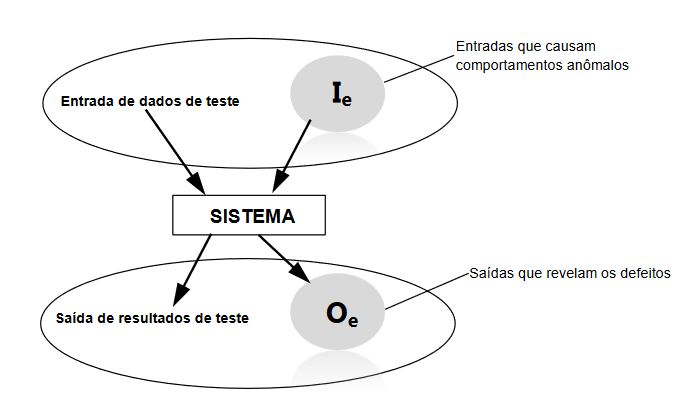
\includegraphics[scale=0.7]{dados/figuras/modelo_entradaSaida.JPG}
	\caption{Um modelo de entrada-saída de teste de programa.}
	Fonte: \cite[p.~145]{SOMMER2011}
	\label{modeloEntradaSaida}
\end{figure}


A Figura \ref{modeloEntradaSaida} apresenta um conjunto de entradas, representadas pelo conjunto \textbf{I}(\textit{input}) que serão processadas pelos sistema a ser testado, entre as entradas do conjunto contém um subconjunto \textbf{Ie} que representa um conjunto de entradas imprecisas e erradas, este conjunto de dados pode causar um erro ou apresentar um defeito de sistema. Então uma bateria de testes é realizada a partir das entradas especificadas gerando o conjunto de saídas \textbf{O}(\textit{output}), alguns dos testes devem apresentar erro pois representam o conjunto de saídas de \textbf{Oe} que é resultante da entrada de \textbf{Ie}. O objetivo dos conjuntos de entradas e saídas de testes e avaliação dos requisitos, já os subconjuntos testam a segurança a falhas e defeitos do sistema.

O teste é apenas parte de um processo de validação e verificação, proporcionando uma etapa importante dentro do processo de desenvolvimento, mas erros podem vir a acontecer, eles não demonstram que o software é livre de falhas, e que ele irá se comportar como o planejado no ambiente para qual foi projetado. É possível que o teste que não foi projetado seja aquele que descobriria uma falha no sistema \cite{SOMMER2011}.

Uma boa estratégia para teste de software é a de aplicação de testes de: baixo nível para verificar se um trecho de código foi implementado corretamente (teste de unidade), testes de integração que verificam a funcionalidade de um componente e a sua incorporação com outros componentes na arquitetura de software; teste de validação que demonstra se os requisitos foram atendidos, e o teste de sistema que aprova o software quando ele é incorporado em sistemas maiores. Cada etapa é realizada com uma serie de técnicas que auxiliam na resolução de problemas e detecção de falhas \cite{PRESMA2016}.

A estratégia de testes pode ser entendida como um espiral, partindo do centro para a sua extremidade passando pelas fases de teste de unidade, integração, validação e sistema. A FIGURA \ref{espiral} mostra a ideia proposta por Pressman.

\begin{figure}[h!]
	\centering
	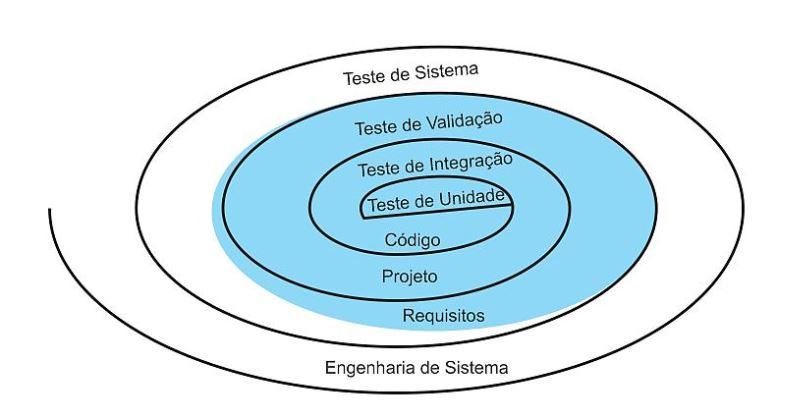
\includegraphics[scale=0.6]{dados/figuras/espiralPres.JPG}
	\caption{Estratégia de teste.}
	Fonte: \cite[p.~470]{PRESMA2016}
	\label{espiral}
\end{figure}

Os testes unitários estão no centro da espiral e representam os fragmentos de código a menor parte de um requisito. Funções\footnote{Conjunto de comandos que realiza uma tarefa específica em um módulo dependente de código.}, classes\footnote{Descrição que abstrai um conjunto de objetos com características similares} e variáveis\footnote{Um objeto (uma posição, frequentemente localizada na memória) capaz de reter e representar um valor ou expressão. } são testados nessa etapa. Conforme se avança na espiral se dá início ao teste de integração de componentes, esta etapa trata de verificar se a integração de diferentes fragmentos do software e suas interfaces\footnote{Recurso que permite a elaboração de códigos flexíveis, diminuindo a amarração do código, permitindo o acesso a atributos e métodos de outras classe sem acessar esta classe diretamente.} não acarretam problemas em funcionalidades já testadas. Seguindo na espiral a validação, já mencionada, trata de validar os requisitos do sistema. Por fim o teste de sistema consiste em validar se todos os componentes integrados e validados se combinam para formar um único produto de software que pode integrar sistemas maiores.

 O processo de teste pode atender várias outras etapas do processo de produção de um software afim de garantir maior qualidade no produto final. De maneira geral os testes podem rastrear defeitos no programa, mas isso não impede que existam defeitos remanescentes \cite{SOMMER2011}.

\subsection{Teste Unitário}

Teste de unidade é o processo que foca nas menores unidades do software, como métodos, classes e variáveis. Neste processo pode-se usar como guia a descrição do projeto para se testar caminhos de controle importantes, e descobrir falhas nos limites dos módulos \cite{PRESMA2016}.

No teste orientado a objetos\footnote{Paradigma de programação baseado no conceito de "objetos", que podem conter dados na forma de campos, também conhecidos como atributos, e códigos, na forma de procedimentos, também conhecidos como métodos.}, devem-se cobrir todas as características  do objeto de modo que todas as operações associadas devem ser testadas. Todos os atributos associados ao objetos devem ser definidos e verificados, e todos os eventos que causam alteração no objeto devem ser testada colocando o objeto em todos os estados possíveis \cite{SOMMER2011}.

O teste de unidade foca em tarefas importantes de um módulo, tais como interface de comunicação, estrutura de dados locais, condições limites, caminhos independentes e caminhos de manipulação de erro, como no esquema da FIGURA \ref{unidade} ilustrada por Pressman.

\begin{figure}[H]
	\centering
	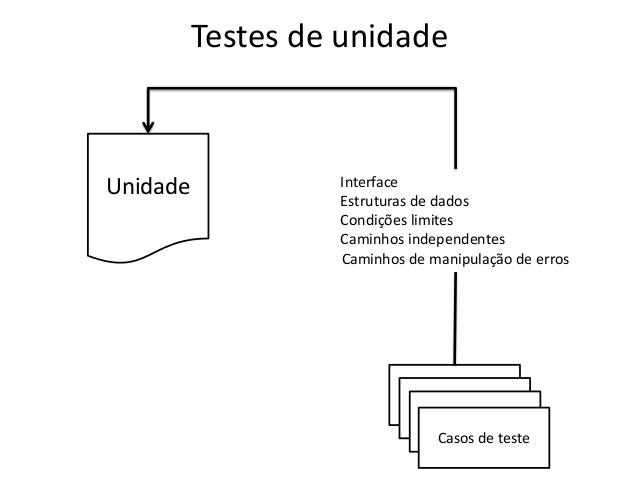
\includegraphics[scale=0.5]{dados/figuras/testeDeUnidade.jpg}
	\caption{Teste de Unidade.}
	Fonte: \cite[p.~474]{PRESMA2016}
	\label{unidade}
\end{figure}

A Figura \ref{unidade} considera os principais objetivos do teste de unidade. O teste de interface do módulo é responsável por testar a comunicação deste módulo com os demais módulos e se o fluxo de dados que percorre a interface entra e sai corretamente, se o fluxo de entrada e saída forem incorretos todos os outros testes irão falhar. A estrutura de dados deve ser testada para garantir que os dados armazenados pelo módulo permaneçam íntegros durante todo o processo de execução do algoritmo. Os valores e condições limites devem ser testados para garantir que o software possa operar nos extremos de sua especificação mantendo a integridade e sua capacidade de processamento. Por fim os testes de manipulação de erro são testados para garantir que uma exceção ou uma falha é tratada e corrigida pelo software \cite{PRESMA2016}.

Teste unitários sempre que possível devem ser automatizados, para quando a aplicação sofrer alguma alteração ou for integrada a um outro componente, os testes possam ser realizados novamente. O uso de \textit{Framework}\footnote{Plataforma de desenvolvimento que contém uma estrutura base para desenvolvimento de soluções em projetos de software.} de automação facilita este processo, como o \textit{JUnit}. Por muitas vezes o objeto que será testado possui dependências em outros objetos que ainda não foram implementados ou não estão disponíveis no ambiente, para o que o processo de teste não atrase é possível a utilização de \textit{Framework} do tipo \textit{mock objects} que simula o comportamento de objetos externos através métodos simulados \cite{SOMMER2011}. 



\subsection{Teste de Componente/Integração}

Os componentes em softwares são compostos de diversos objetos que interagem. Os testes em componentes compostos devem focar nas interfaces de comunicação. Deve-se garantir que quando objetos diferentes são integrados eles se comuniquem de acordo com o especificado. Os testes de unidade não cobrem os testes de componente pois avaliam a interação de um único objeto, já os testes de componente avaliam a interação de diversos componente pelas suas interfaces, o que pode gerar comportamento anômalos dos objetos já testados \cite{SOMMER2011}.


Os testes em interface são os mais difíceis de serem realizados pois problemas podem surgir somente em uma situação inesperada \cite{SOMMER2011}. Dados podem ser perdidos, funções de objetos diferentes combinadas podem não produzir o efeito desejado, estruturas globais podem apresentar problemas, estes entre outros erros podem surgir na integração de componentes \cite{PRESMA2016}.


Os testes unitarios comuns não são muito eficientes em encontrar erros de interface. Inspeções de código e validações de funcionalidades do projeto podem ser mais eficientes para revelar os erros. Inspeções podem se focar no comportamento da interface durante a execução e integração com outros componentes, o comportamento deve ser validado de acordo com a especificação \cite{SOMMER2011}. O objetivo do teste de componente é construir uma estrutura de software baseado em unidades testadas.


 
\subsection{Teste de Validação}

O teste de validação começa quando o teste de componentes termina. O software está em um estado parcialmente acabado onde já é possivel processar entradas e produz saídas. O teste de validação de software se trata de uma série de comparações do produto já implementado com os requisitos propostos no início do desenvolvimento. A validação pode ser definida como a maneira de atingir razoavelmente bem o que foi especificado pelo cliente nos requisitos do software \cite{PRESMA2016}.  


No caso de softwares personalizados para clientes específicos, o teste de validação pode ser realizado pelo cliente juntamente com a equipe de desenvolvimento. O cliente recebe uma versão inacabada do software, ele testa as funcionalidades desenvolvidas até o momento e avalia se os requisitos pedidos foram atendidos. Se o  desvio dos requisitos foram descobertos é criada uma lista de deficiência e deve se estabelecer um método para solucionar os desvios \cite{PRESMA2016}.


\subsection{Teste de Sistema}

A última etapa de teste se foca na interação de componentes para dar início a uma nova versão do sistema, e em seguida é dado início à bateria de testes do sistema integrado. Apesar de se parecer com o teste de componentes, o teste de sistema se preocupa com a interação e comunicação do sistema com outro diversos componentes, software de terceiros, hardware, rede, informação e pessoas. Nesta etapa é testada a comunicação entre os diversos componente, e suas interfaces se são compatíveis, se interagem corretamente e se transferem os dados corretamente no momento certo \cite{SOMMER2011}.


Uma boa estratégia para teste de sistema é criar testes de interação com o sistema baseados em casos de uso. Geralmente cada caso de uso representa uma tarefa mais complexa, o que exige uma série de transações do sistema. Testes de sistema geralmente são mais difíceis de se realizar pois podem produzir saídas muito grandes e de difícil previsão, mais é possível analisar uma saída e verificar sua credibilidade tendo como base uma previsão realizada com antecedência \cite{SOMMER2011}.



\section{JUNIT 5 FRAMEWORK}

O  \textit{JUnit} é uma plataforma de execução de testes na JVM (\textit{Java virtual machine}), que utiliza uma estrutura de anotações para identificar métodos que especificam um teste. A nova arquitetura do \textit{JUnit} 5 é dívida em módulos que são agrupados em três pacotes que compõem o \textit{framework}. 

\begin{itemize}

\item O \textit{JUnit Plataform} contém elementos estruturais para execução de testes. Esta plataforma implementa uma API de \textit{TestEngine}\footnote{Plataforma que permite a execução de testes baseados em JUnit.} possibilitando que outros \textit{frameworks} possam ser executados. Por exemplo, a \textit{TestEngine} possibilita a execução de testes escritos usando o modelo de programação \textit{JUnit Jupiter} \cite{Junit}. 


\item O \textit{JUnit Jupiter} é o modelo de programação e extensão de API utilizado para criação de testes no \textit{JUnit} 5, é neste pacote que estão definidas as anotações e classes que são necessárias para a construção dos testes, como a anotação \textit{@Test} e várias outras \cite{Junit}.


\item O \textit{JUnit Vintage} é um pacote que provê uma \textit{TestEngine} para execução de testes baseados em versões do \textit{JUnit} 3 e \textit{JUnit} 4 da plataforma \cite{Junit}.


\end{itemize}


Cada módulo é distribuído como um artefato\footnote{Um subproduto concreto produzido durante o desenvolvimento de software.} e publicado em diversas plataformas de IDEs (\textit{Integrated development environment}) populares (\textit{IntelliJ IDEA , Eclipse , NetBeans e Visual Studio Code}), e ambientes de construção\footnote{Conjunto de ferramentas criadas para auxiliar a criação e desenvolvimento de um software.} (\textit{Gradle , Maven e Ant}). O \textit{JUnit} 5 requer o Java 8. No entanto, ainda é possível testar o código que foi compilado com versões anteriores do JDK (\textit{Java Development Kit}) \cite{Junit}.


Com o \textit{Junit} é possível criar testes unitários para verificar as funcionalidades de classes e seus métodos. Assim é possível automatizar a execução de todos os testes unitários de forma que quando for criada uma nova versão estável do sistema, o \textit{framework} execute todos os testes unitários para garantir a integridade e estabilidade do sistema desenvolvido.


% \subsection{Adicionando JUnit Usando Maven }

% Para a utilização do \textit{Junit} basta baixar os artefatos desejados a IDE de preferencia ou adicionar as dependências com a ferramenta de gerenciamento de dependências opcional do usuário. A FIGURA \ref{mvn} ilustram a importação\footnote{Recurso que permite amarrar o código de uma classe ou método externo a outras classes.} do pacote \textit{JUnit Jupiter} pela ferramenta de gerenciamento de dependências \textit{Maven}. 

% \begin{figure}[h!]
% 	\centering
% 	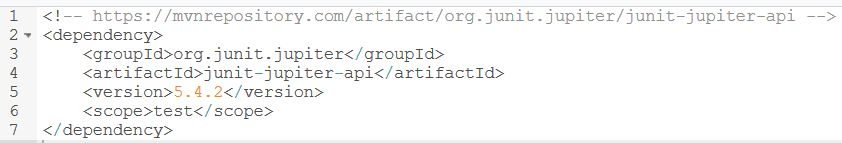
\includegraphics[scale=0.7]{dados/figuras/mvnJu.JPG}
% 	\caption{Importação do Pacote JUnit Jupiter API Utilizando Maven.}
% 	Fonte: \cite[Link:~https://mvnrepository.com/artifact/org.junit.jupiter/junit-jupiter-api/5.4.2]{Maven}
% 	\label{mvn}
% \end{figure}

% A FIGURA \ref{mvn} apresenta a importação do pacote \textit{JUnit Jupiter} onde cada linha tem a sua seguinte função. 

% \begin{itemize}
  
% \item[1]: é indicado o repositório central onde são armazenadas todas as versões do pacote importado. 

% \item[2]: a \textit{tag} \textit{<dependencies>} é aberta, é dentro desta \textit{tag} que cada dependência é definida individualmente, 


% \item[3]: a \textit{tag} \textit{<groupId>} é aberta e fechada, ela é o identificador único do pacote \textit{"org.junit.jupiter”} responsável por indicar a coordenada \textit{Mavem} do projeto.

% \item[4]: a \textit{tag} \textit{<artifactId>} é aberta e fechada, ela é geralmente o nome pelo qual o projeto é conhecido \textit{"junit-jupiter-api"},  ela juntamente com a \textit{tag} \textit{<groupId>} é responsável separar o projeto de todos os outros do repositório central.


% \item[5]: alterações no código geram versões diferentes do mesmo pacotes a \textit{tag} \textit{<version>} \textit{"5.4.2"} indica quais alterações feitas no código e devem ser baixadas.
 
% \item[6]: esta \textit{tag} \textit{<scope>} faz referência ao tipo de trabalho \textit{"test"} que será realizado pelo pacote, e limita a transitividade de um pacote.


% \item[7]: é responsável por fecha a chave de \textit{tags} \textit{<dependency>}.

% \end{itemize}


% Para que a importação seja realizada com sucesso a dependência deve ser declarada em um arquivo de POM.xml (Project Object Model) que contem a lista de dependências do projeto, este é a peça fundamental de um projeto Maven \cite{Maven}.



\subsection{Utilizando JUnit}

O \textit{JUnit} utiliza uma referência por anotações. Essas funcionam como uma estrutura de cascata que define quais elementos devem ser executados e criados antes dos testes terem início. Elas também podem ser usadas como filtro para indicar quais testes devem ser realizados primeiro, caso o processo de teste seja muito extenso e custoso. 
As principais anotações são apresentadas na Tabela \ref{tab:tags1} no site do \textit{JUnit}:


\begin{table}[!h]
\caption[Anotações JUnit]{Anotações JUnit.}
\label{tab:tags1}
\begin{tabular}{|l|l|}
\hline
\textbf{Anotação (Tag)} & \textbf{Descrição}                                                                                                                                           \\ \hline
@Test                   & \begin{tabular}[c]{@{}l@{}}Indica que um método é um método de teste. Ao contrário da \\ anotação @Test do JUnit 4, essa anotação não declara \\ nenhum atributo, já que as extensões de teste no JUnit Jupiter \\ operam com base em suas próprias anotações dedicadas.\end{tabular} \\ \hline
@BeforeEach             & \begin{tabular}[c]{@{}l@{}}Indica que o método anotado deve ser executado antes de \\ cada  método @Test , @RepeatedTest , \\ @ParameterizedTest ou @TestFactory na classe atual\end{tabular}                                                                                         \\ \hline
@AfterEach              & \begin{tabular}[c]{@{}l@{}}Indica que o método anotado deve ser executado após \\ cada método @Test , @RepeatedTest , \\ @ParameterizedTest ou @TestFactory na classe atual\end{tabular}                                                                                              \\ \hline
@TestInstance           & \begin{tabular}[c]{@{}l@{}}Usado para configurar o ciclo de vida da instância de \\ teste para a classe de teste anotada.\end{tabular}                                                                                                                                                \\ \hline
@DisplayName            & \begin{tabular}[c]{@{}l@{}}Declara um nome de exibição personalizado para a classe \\ de teste ou método de teste.\end{tabular}                                                                                                                                                       \\ \hline
@Disabled               & Usado para desabilitar uma classe de teste ou método de teste.                                                                                                                                                                                                                        \\ \hline
@BeforeAll              & \begin{tabular}[c]{@{}l@{}}Indica que o método anotado deve ser executado antes de todos os \\ métodos @Test , @RepeatedTest , @ParameterizedTest e \\ @TestFactory na classe atual.\end{tabular}                                                                                     \\ \hline
@AfterAll               & \begin{tabular}[c]{@{}l@{}}Indica que o método anotado deve ser executado após todos os\\ métodos @Test , @RepeatedTest , @ParameterizedTest e \\ @TestFactory na classe atual.\end{tabular}                                                                                          \\ \hline
\end{tabular}
\\ Fonte: \cite[https:~//junit.org/junit5/docs/current/user-guide/overview]{Junit}
\end{table}

É possível encontrar todas as anotações e suas especificações no pacote \textit{org.junit.jupiter.api} no site oficial do \textit{JUnit}.



A Figura \ref{JUnit} apresenta um teste simples sendo implementado utilizando as ferramentas do \textit{JUnit} : 

\begin{figure}[!h]
	\centering
	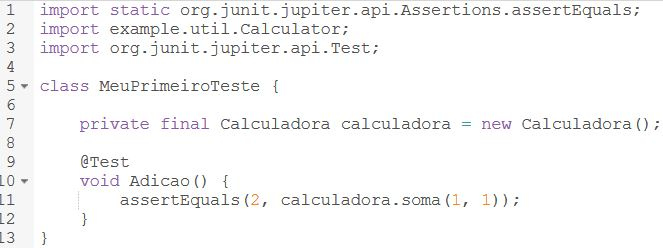
\includegraphics[scale=0.9]{dados/figuras/tesLine.JPG}
	\caption{Teste utilizando JUnit.}
	\label{JUnit}
\end{figure}

O trecho de código da Figura \ref{JUnit} apresenta um teste simples. Na linha 2 é realizada a importação da classe \textit{"Calculadora"}, que se trata de uma classe concreta que implementa o método “soma”, este método recebe dois valores inteiros como parâmetro e retorna a soma dos dois valores.  O restante do código possui as seguintes características:

\begin{itemize}

\item[1]:  é importada a função de \textit{"assertEquals"} do pacote \textit{JUnit}, esta função e responsável por comparar dois valores, o primeiro valor é o valor esperado de uma operação, resultado, ou estado. O segundo valor é o valor resultante da chamada de uma função, classe, ou variável que se deseja testar. 

\item[2]: realiza a importação da classe \textit{"Calculadora"} que será testada. 

\item[3]: realiza a importação do pacote de testes \textit{JUnit} onde se encontram as \textit{tags} de anotações é os metodos\footnote{Determinam o comportamento dos objetos de uma classe e são análogos às funções.} do \textit{Framework}. 

\item[5]: a classe principal \textit{"MeuPrimeiroTeste"} é aberta. 

\item[7]: é instanciado\footnote{Criar um novo objeto do mesmo tipo dessa classe} um objeto do tipo \textit{"Calculadora"} na variável \textit{"calculadora"}. 

\item[9]: é utilizada a anotação \textit{@Test}, esta anotação sinaliza que o método a seguir é um método que deve realizar um teste. 

\item[10]: o método de nome \textit{"Adicao"} é declarado, sendo do tipo \textit{"void"} (sem retorno). 

\item[11]: a função importada \textit{"assertEquals"} é chamada, a ela é passado o valor inteiro 2, e em seguida a função \textit{"calculadora.soma(1,1)"}. A excecução do progama segue com a chamada do metodo  \textit{"soma"} realizada pelo objeto instanciado na variável "calculadora". A função \textit{"soma"} chamada recebe dois valores, realiza a soma e retorna o resultado. O retorno da função \textit{"soma"} é agurdado para comparação com o primeiro valor passado a função \textit{"assertEquals"}.

\item[12]: o método \textit{"Adicao"} é fechado.

\item[13]: a classe principal é fechada.

\end{itemize}

Caso o retorno da função \textit{"soma"} seja um inteiro "2", o mesmo resultado esperado pelo \textit{assertEquals}, o resultado do teste será verdadeiro, então logo o teste é aprovado. Caso a função \textit{"soma"} retorne outro valor diferente de um inteiro "2"  o resultado será falso, logo o teste é reprovado. 


    Mais funções do \textit{Framework JUnit} serão explorados ao longo deste trabalho.


\section{MOCKITO FRAMEWORK}


\textit{Mockito} é um \textit{framework} de simulação baseado em JAVA que é utilizado para testes unitários em aplicativos. Um teste de unidade deve testar a funcionalidade isoladamente. Todos os efeitos colaterais possíveis de outras classes ou do sistema devem ser eliminados para um teste de unidade  \cite{Mockito}. 


O \textit{Mockito} é usado para simular interfaces, de modo que uma funcionalidade fictícia possa ser adicionada a uma interface simulada que pode ser usada no teste de unidade. O objetivo principal é no sentido de que os objetos simulados são criados para imitar objetos reais de maneira controlada. Os objetos simulados são basicamente uma versão simulada do objeto original que é programaticamente\footnote{Que possui um plano de atividade para realizar uma determinada função.} criado para verificar o comportamento de outro objeto. O princípio da programação orientada a objetos é a comunicação e o relacionamento entre objetos, à medida que o contexto se amplia, a unidade individual como um objeto pode ter que ser expandida em módulos. Portanto, quando se testa um componente, é possível testar os módulos como uma unidade individual e seu relacionamento, o ponto é que um objeto individual raramente faz sentido em um programa. Objetos funcionam em relação. Assim, escolher uma unidade para testar é tão necessário quanto testar seu relacionamento. O objeto \textit{mocking} é uma técnica para testar unidades isoladamente, simulando suas unidades dependentes.


% \subsection{Adicionando Mockito Usando Maven}

% Para a utilização do \textit{Mockito} basta baixar os artefatos desejados a IDE de preferencia ou adicionar as dependências com a ferramenta de gerenciamento de dependências opcional do usuário. A FIGURA \ref{mvn2} ilustram a importação do pacote \textit{Mockito 2.0.2-beta} pela ferramenta de gerenciamento de dependências \textit{Maven}. 

% \begin{figure}[H]
% 	\centering
% 	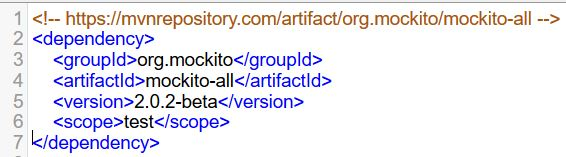
\includegraphics[]{dados/figuras/mockito.JPG}
% 	\caption{Importação do Pacote Mockito 2.0.2-beta Utilizando Maven.}
% 	Fonte: \cite[https:~//mvnrepository.com/artifact/org.mockito/mockito-all/2.0.2-beta]{Maven}
% 	\label{mvn2}
% \end{figure}

% A FIGURA \ref{mvn2} apresenta a importação do pacote \textit{Mockito 2.0.2-beta} onde cada linha e tem a sua seguinte função: 

% \begin{itemize}
  
% \item[1]: é indicado o repositório central onde são armazenadas todas as versões do pacote importado. 

% \item[2]: a \textit{tag} \textit{<dependencies>} é aberta, é dentro desta \textit{tag} que cada dependência é definida individualmente, 

% \item[3]: a \textit{tag} \textit{<groupId>} é aberta e fechada, ela é o identificador único do pacote \textit{"org.mockito”} responsável por indicar a coordenada \textit{Mavem} do projeto.

% \item[4]: a \textit{tag} \textit{<artifactId>} é aberta e fechada, ela é geralmente o nome pelo qual o projeto é conhecido \textit{"mockito-all"},  ela juntamente com a \textit{tag} \textit{<groupId>} é responsável separar o projeto de todos os outros do repositório central.


% \item[5]: alterações no código geram versões diferentes do mesmo pacotes a \textit{tag} \textit{<version>} \textit{"2.0.2-beta"} indica quais alterações feitas no código e devem ser baixadas.
 
% \item[6]: esta \textit{tag} \textit{<scope>} faz referência ao tipo de trabalho \textit{"test"} que será realizado pelo pacote, e limita a transitividade de um pacote.


% \item[7]: é responsável por fecha a chave de \textit{tags} \textit{<dependency>}.

% \end{itemize}


% Para que a importação seja realizada com sucesso a dependência deve ser declarada em um arquivo de \textit{POM.xml (Project Object Model)} que contem a lista de dependências do projeto, este é a peça fundamental de um projeto \textit{Maven} \cite{Maven}.



\subsection{Utilizando Mockito}

O \textit{Mockito} permite a utilização de vários métodos para a criação de objetos simulados, desde \textit{tags} de anotações a métodos estáticos. 
Na utilização de \textit{tags} de anotação como \textit{@Mock}, é necessário que se defina o comportamento dos objetos anotados e em seguida invoque o método \textit{MockitoAnnotations.initMocks(this)} para preencher os campos anotados.
Na utilização de métodos estáticos, adicionando o \textit{org.mockito.Mockito.*;} é possível trabalhar com importação estática e utilizar os métodos do pacote \textit{mockito} diretamente nos testes. As importações estáticas permitem que membros estáticos sejam chamados, isto é, métodos e campos de uma classe podem ser chamados diretamente \cite{Mockito}, \cite{Javadoc}.
 A FIGURA \ref{mockito} é um exemplo de teste utilizando importação estática do pacote \textit{Mockito}.




A FIGURA \ref{mockito} traz na linha de código 8 a classe \textit{Calculadora}. Esta classe se trata de uma \textit{interface}, ela possui a declaracção do método \textit{"add"} que recebe dois valores inteiros. A classe não possui comportamento algum, todo e qualquer comportamento que se espera dessa classe deve ser simulado ou implementado em outra classe concreta. O restante do código possui as seguintes características:

\begin{figure}[H]
	\centering
	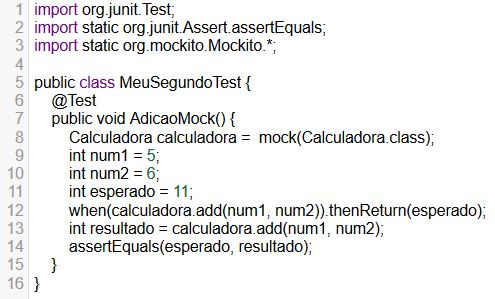
\includegraphics[scale=0.9]{dados/figuras/testeMock.JPG}
	\caption{Teste utilizando Mockito.}
	\label{mockito}
\end{figure}


\begin{itemize}

\item[1]: realiza a importação do pacote de testes \textit{JUnit} onde se encontram as \textit{tags} de anotações e os metodos do \textit{Framework}. 

\item[2]:  é importada a função de \textit{"assertEquals"} do pacote \textit{JUnit}, esta função e responsável por comparar dois valores, o primeiro valor é o valor esperado de uma operação, resultado, ou estado. O segundo valor é o valor resultante da chamada de uma função, classe, ou variável que se deseja testar. 

\item[3]: realiza a importação do pacote \textit{"mockito.Mockito.*"}, onde estão contidos todos os métodos estáticos do pacote e as \textit{tags} de anotações. 


\item[5]: a classe principal \textit{"MeuSegundoTeste"} é aberta. 

\item[6]: é utilizada a anotação \textit{@Test}, esta anotação sinaliza que o método a seguir é um método que deve realizar um teste. 

\item[7]: o método de nome \textit{"AdicaoMock"} é declarado, sendo do tipo \textit{"void"} (sem retorno). 


\item[8]: é instanciado um objeto do tipo \textit{"Calculadora"} na variável \textit{"calculadora"}. Como o objeto que se deseja instanciar se trata de uma interface e não possui comportamento definido, é utilizado a função \textit{“mock”} do pacote \textit{"mockito.Mockito.*"} para que o objeto instanciado possua um comportamento fictício. 

\item[9]: a variável do tipo inteiro \textit{“num1”} é declarada. Ela recebe o valor inteiro "5". 

\item[10]: a variável do tipo inteiro \textit{“num2”} é declarada. Ela recebe o valor inteiro "6".

\item[11]: a variável do tipo inteiro \textit{“esperado”} é declarada. Ela recebe o valor inteiro "11". 

\item[12]: O método \textit{“when().thenReturn()”} do pacote \textit{"mockito.Mockito.*"}  é utilizado para definir o comportamento do objeto \textit{Mock}, o que ele deve fazer em certas situações.
O comando \textit{“when”}  determina qual método deve ser chamado no futuro e quais parâmetros ele deve receber. A ele passamos a função e os parâmetros \textit{"calculadora.add(num1,num2)"}. O \textit{“thenReturn”} diz qual será o valor devolvido quando o método definido no comando \textit{“when”} for chamado. O retorno definimos sendo a variável \textit{“esperado”}.


\item[13]: a variável do tipo inteiro \textit{“resultado”} é declarada. Ela recebe o retorno da função \textit{"calculadora.add(num1,num2)"}. A execução do progama segue com a chamada do metodo  \textit{"add"} realizada pelo objeto \textit{mocado}\footnote{Simula o comportamento de um outro objeto.} instanciado na variável \textit{"calculadora"}. A função \textit{"add"} chamada possui o comportamento definido em \textit{“whem}”  e \textit{“thenReturn"}, recebe dois valores, realiza a soma, e retorna o resultado.

\item[14]: a função importada \textit{assertEquals} é chamada, a ela é passado a variável \textit{“esperado”}, e em seguida a a variável \textit{“resultado}”. A função realiza a comparação entre as variáveis.

\item[15]: o método \textit{"AdicaoMock"} é fechado.

\item[16]: a classe principal é fechada.

\end{itemize}

Caso o retorno da função \textit{"add"} seja um inteiro "11", o mesmo resultado da variável \textit{“esperado”} o resultado do teste será verdadeiro, então logo o teste é aprovado. Caso a função \textit{"add"}  retorne outro valor diferente de um inteiro "11"   o resultado será falso, logo o teste é reprovado. 


    Mais funções do \textit{FrameWork Mockito} serão explorados ao longo deste trabalho.

\section{SPRING FRAMEWORK TEST}

O \textit{Spring Framework} é uma ferramenta que fornece suporte para diversos tipos de aplicações em diferentes etapas do desenvolvimento. Embora testes de unidade busquem testar minuciosamente trechos de código, é importante poder realizar alguns testes de integração sem exigir a implantação do aplicativo em  servidores ou conectá-los com a infraestrutura corporativa \cite{spring}. O \textit{spring-boot-test} é um modlo dedicado somente para testes de integração de aplicativos \textit{Spring Boot}.


Os pacotes de testes contidos na biblioteca do \textit{spring-framework-test} não dependem de servidores de aplicações ou ambientes de execuções. Os testes de implantação são mais lentos do que os testes de unidade, porém, são mais rápidos do que os testes de  interface com Selênio, e equivalentes aos testes remotos que dependem da implantação da aplicação em um servidor. O \textit{Spring Framework Test} fornece suporte a testes de unidade e integração, ele utiliza a orientação por anotações o que permite a criação de testes em vários ambientes, incluindo \textit{JUnit} \cite{spring}. O suporte de testes de integração do \textit{Spring} fornece: 

\begin{itemize}
    \item Gerenciamento de contexto\footnote{Conjunto de dados mínimos usados por uma tarefa que deve ser salvo para permitir uma interrupção da tarefa e a posteriormente a continuação desta tarefa no ponto que ela foi interrompida sem perca de dados.} e cache\footnote{Área de memória onde é mantida uma cópia temporária de dados}, ou seja, o aplicativo é carregado em apenas uma JVM e a partir desta instância todos os testes são executados, o que reduz o tempo de execução dos testes, já que evita que o aplicativo seja carregado toda vez que um teste for executado  \cite{spring}. 


\item Injeção de dependências a partir do contexto de execução de uma aplicação fornece instancias de classes em tempo de execução para outros cenários de testes  \cite{spring}. 


\item Gerenciamento de transações esta funcionalidade garante que as modificações realizadas em base de dados não persistam após a execução de um teste  \cite{spring}. 



\item Classes de suporte para testes de integração o \textit{Spring Framework} fornece várias classes de suporte abstratas que simplificam a criação de testes de integração. Essas classes fornecem ganchos bem definidos na estrutura de teste, bem como variáveis e métodos de instância convenientes  \cite{spring}.

\end{itemize}


% \subsection{Adicionando Spring Boot Test Usando Maven}

% Para a utilização do \textit{Spring Boot Test} basta cria o projeto no site \textit{Spring Initializr} \url{https://start.spring.io/},  ou adicionar as dependências com a ferramenta de gerenciamento de dependências opcional do usuário. A FIGURA \ref{springfig} ilustram a importação do pacote \textit{Spring Boot Starter Test} pela ferramenta de gerenciamento de dependências \textit{Maven}. 

% \begin{figure}[H]
% 	\centering
% 	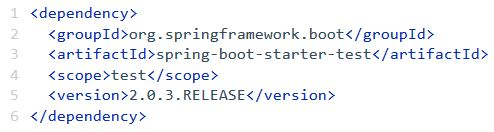
\includegraphics[]{dados/figuras/mavenSpring.JPG}
% 	\caption{Importação do Pacote Spring Boot Starter Test Utilizando Maven.}
% 	Fonte: \cite[https:~//mvnrepository.com/artifact/org.springframework.boot/spring-boot-starter-test/2.0.3.RELEASE]{Maven}
% 	\label{springfig}
% \end{figure}

% A FIGURA \ref{springfig} apresenta a importação do pacote \textit{Spring Boot Starter Test} onde cada linha de código tem a sua seguinte função: 

% \begin{itemize}

% \item[1]: a \textit{tag} \textit{<dependencies>} é aberta, é dentro desta \textit{tag} que cada dependência é definida individualmente, 

% \item[2]: a \textit{tag} \textit{<groupId>} é aberta e fechada, ela é o identificador único do pacote \textit{"org.springframework.boot”} responsável por indicar a coordenada \textit{Mavem} do projeto.

% \item[3]: a \textit{tag} \textit{<artifactId>} é aberta e fechada, ela é geralmente o nome pelo qual o projeto é conhecido \textit{"spring-boot-starter-test"},  ela juntamente com a \textit{tag} \textit{<groupId>} é responsável separar o projeto de todos os outros do repositório central.


% \item[4]: alterações no código geram versões diferentes do mesmo pacotes a \textit{tag} \textit{<version>} \textit{"2.0.3.RELEASE"} indica quais alterações feitas no código e devem ser baixadas.
 
% \item[5]: esta \textit{tag} \textit{<scope>} faz referência ao tipo de trabalho \textit{"test"} que será realizado pelo pacote, e limita a transitividade de um pacote.


% \item[6]: é responsável por fecha a chave de \textit{tags} \textit{<dependency>}.

% \end{itemize}


% Para que a importação seja realizada com sucesso a dependência deve ser declarada em um arquivo de \textit{POM.xml (Project Object Model)} que contem a lista de dependências do projeto, este é a peça fundamental de um projeto Maven \cite{Maven}.


\subsection{Utilizando Spring Boot Test}

O \textit{Spring Framework} fornece um conjunto de anotações específicas do \textit{Spring} que podem ser usadas em testes de unidade e testes de integração em conjunto com o \textit{framework TestContext}.  A FIGURA \ref{springfig2} traz um exemplo do uso de anotações utilizando o spring framework test.

\begin{figure}[H]
	\centering
	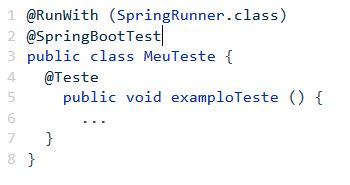
\includegraphics[]{dados/figuras/testeSpring.JPG}
	\caption{Anotações Utilizando o Spring Framework Test.}
	\label{springfig2}
\end{figure}

O trecho de código da FIGURA \ref{springfig2} apresenta a declaração de um teste que utiliza as anotações do \textit{Spring Boot Test}. Cada linha possui a seguinte função:

\begin{itemize}

\item[1]: A anotação \textit{"@RunWith(SpringRunner.class)"}, oferece integração total com o \textit{JUnit} 4 ou superior. Esta anotação define um padrão de configuração personalizado para a classe chamada \cite{spring}. 

\item[2]: O \textit{Spring Boot} fornece a anotação \textit{"@SpringBootTest"}, ela define metadados de nível de classe que são usados para carregar e configurar uma aplicação para testes de interface, ou seja,  carrega as alocações e os recursos necessários para a execução do aplicativo e das classes anotadas usadas no contexto da aplicação \cite{spring}.   

\item[3]: a classe principal \textit{"MeuTeste"} é aberta. 

\item[4]: é utilizada a anotação \textit{"@Test"}, esta anotação sinaliza que o método a seguir é um método que deve realizar um teste. 

\item[5]: o método de nome \textit{"exemploTeste"} é declarado, sendo do tipo \textit{"void"} (sem retorno). 

\item[6]:O corpo do método deve ser implementado aqui.

\item[7]: o método \textit{"exemploTeste"} é fechado.

\item[8]: a classe principal é fechada.

\end{itemize}

O documento completo com todas as anotações, métodos e atributos disponíveis pelo \textit{framework} podem ser encontrados no site oficial do \textit{FrameWork Spring Test} \cite{spring}. Mais funções do \textit{FrameWork} serão explorados ao longo deste trabalho.

         % Revisão de Literatura
% % METODOLOGIA------------------------------------------------------------------

\chapter{PROPOSTA}
\label{chap:metodologia}

Nesta seção são apresentadas as tecnologias, ferramentas necessárias, os requisitos e  classes a serem testadas  do aplicativo.

\section{Manejo Integrado de Pragas (MIP)}
        
O MIP tem como objetivo criar uma ferramenta capaz de auxiliar o constante monitoramento da lavoura, buscando manter a presença de pragas e doenças sempre abaixo do nível de dano à cultura. A estratégia não é eliminar completamente os agentes causadores de dano, mas reduzi-los a um ponto em que seus inimigos naturais presentes na plantação hajam sobre suas presas, favorecendo o equilíbrio natural desfeito pela plantação e pelo uso de defensores agrícolas. Para atingir seu objetivo, a ferramenta depende de coletas de dados semanais coletados através da metodologia do pano-de-batida\footnote{Técnica de coleta pragas em lavouras.} para acompanhar o nível populacional das principais pragas da lavoura. 


O sistema de coleta e análise de dados do MIP auxilia no acompanhamento das atividades de coleta e análise de dados das lavouras monitoradas pelo EMATER. O sistema também permite o gerenciamento de dados relacionados à coleta, como macrorregiões, regiões, produtores, safras, técnicos e pragas. 

% Para atingir esse objetivo esta ferramenta irá criar e administrar um banco de dados que possibilitará armazenar todas as informações necessárias para o gerenciamento interno de cada unidade e suas respectivas particularidades. Além de fornecer acesso a aplicação através da comunicação cliente servidor\footnote{Estrutura de aplicação distribuída que distribui as tarefas e cargas de trabalho entre os fornecedores de um recurso, e os requerentes dos recursos.}. 



\section{MODELO DO SISTEMA}
Nesta seção, serão apresentados os requisitos funcionais e os principais artefatos gerados para o desenvolvimento da aplicação.

\subsection{Requisitos Funcionais}
Os requisitos são exigências, solicitações, desejos e necessidades que um software deve materializar. A Tabela \ref{tabela-requisitos} identifica os requisitos funcionais de forma abrangente.  

\begin{table}[H]
    \caption[Requisitos Funcionais do Sistema]{Requisitos Funcionais do Sistema.
    \label{tabela-requisitos}}
\begin{tabular}{|l|l|l|l|}
\hline
ID    & Requisito                                                                                 & Descrição                                                                                                                                                                                                                                                                                                                                                                                          & Prioridade \\ \hline
RF001 & \begin{tabular}[c]{@{}l@{}}Gerenciar \\ Macrorregião\end{tabular}                         & \begin{tabular}[c]{@{}l@{}}O sistema deve permitir ao usuário em uma\\ única tela listar registros existentes, cadastrar \\ uma nova macrorregião e alterar ou excluir \\ uma já existente.\end{tabular}                                                                                                                                                                                           & Essencial  \\ \hline
RF002 & \begin{tabular}[c]{@{}l@{}}Gerenciar \\ Região\end{tabular}                               & \begin{tabular}[c]{@{}l@{}}O sistema deve permitir ao usuário em uma \\ única tela listar registros existentes, cadastrar \\ uma nova região e alterar ou excluir uma já \\ existente.\end{tabular}                                                                                                                                                                                                & Essencial  \\ \hline
RF003 & \begin{tabular}[c]{@{}l@{}}Gerenciar \\ Produtores\end{tabular}                           & \begin{tabular}[c]{@{}l@{}}O sistema deve permitir ao usuário em uma \\ única tela listar registros existentes, cadastrar \\ um novo produtor e alterar ou excluir um \\ já existente.\end{tabular}                                                                                                                                                                                                & Essencial  \\ \hline
RF004 & \begin{tabular}[c]{@{}l@{}}Gerenciar \\ Responsáveis \\ Técnicos\end{tabular}             & \begin{tabular}[c]{@{}l@{}}O sistema deve permitir ao usuário em uma \\ única tela listar registros existentes, cadastrar \\ um novo responsável técnico e alterar ou\\ excluir um já existente.\end{tabular}                                                                                                                                                                                      & Essencial  \\ \hline
RF005 & \begin{tabular}[c]{@{}l@{}}Gerenciar \\ Unidades de \\ Referência\end{tabular}            & \begin{tabular}[c]{@{}l@{}}O sistema deve permitir ao usuário em uma \\ única tela listar registros existentes, cadastrar \\ uma nova unidade de referência e alterar ou \\ excluir uma já existente.\end{tabular}                                                                                                                                                                                 & Essencial  \\ \hline
RF006 & \begin{tabular}[c]{@{}l@{}}Gerenciar \\ Safra\end{tabular}                                & \begin{tabular}[c]{@{}l@{}}O sistema deve permitir ao usuário em uma \\ única tela listar registros existentes, cadastrar \\ uma nova safra, alterar ou excluir uma \\ já existente.\end{tabular}                                                                                                                                                                                                  & Essencial  \\ \hline
RF007 & \begin{tabular}[c]{@{}l@{}}Gerenciar \\ UR's \\ Participantes \\ da Pesquisa\end{tabular} & \begin{tabular}[c]{@{}l@{}}O sistema deve permitir ao usuário cadastrar \\ uma nova unidade de referência que participara \\ da pesquisa ou excluir uma participante \\ já cadastrada.\end{tabular}                                                                                                                                                                                                & Essencial  \\ \hline
RF008 & \begin{tabular}[c]{@{}l@{}}Gerenciar \\ Insetos Pragas\end{tabular}                       & \begin{tabular}[c]{@{}l@{}}O sistema deve permitir ao usuário em uma \\ única tela listar registros existentes, cadastrar \\ um novo inseto praga e alterar ou excluir \\ um já existente.\end{tabular}                                                                                                                                                                                            & Essencial  \\ \hline
RF009 & \begin{tabular}[c]{@{}l@{}}Gerenciar \\ Flutuação \\ das Pragas\end{tabular}              & \begin{tabular}[c]{@{}l@{}}O sistema deve listar as safras que estão \\ participando da pesquisa de flutuação de pragas,\\ deve permitir ao usuário registrar uma nova \\ amostra de flutuação populacional das pragas \\ que foram encontradas em uma em uma safra,\\ deve permitir a listagem dos detalhes de cada \\ amostra registrada e a exclusão de amostras \\ já existentes.\end{tabular} & Essencial  \\ \hline
\end{tabular}
\end{table}

\subsection{Especificação dos Requisitos Funcionais}

A Tabela \ref{especificacaoDosRequisitos} apresenta a descrição dos requisitos funcionais de forma detalhada, como deverão ser executados e quais exceções que impedem a sua execução. Os requisitos especificados que foram identificados devem ser testados e validados. 

% Please add the following required packages to your document preamble:
% \usepackage{multirow}

\begin{table}[H]
\centering
\caption{Especificação dos Requisitos Funcionais do Sistema}
\label{especificacaoDosRequisitos}
\begin{tabular}{|l|l|}                                                                                                                                                      \hline
RS001                                                    & Listar macrorregião.                                                                                                                                                                                                                                                                                                                                                                     \\ \hline
Referencia                                               & {[}Gerenciar Macrorregião. RF001{]}.                                                                                                                                                                                                                                                                                                                                                     \\ \hline
Sumario                                                  & \begin{tabular}[c]{@{}l@{}}O requisito é responsável por listar todas as macrorregiões \\ cadastradas no sistema.\end{tabular}                                                                                                                                                                                                                                                           \\ \hline
\begin{tabular}[c]{@{}l@{}}Pré-\\ Condições\end{tabular} & \begin{tabular}[c]{@{}l@{}}O usuário deve efetuar o login no sistema, deve haver uma ou mais\\ macrorregiões cadastradas.\end{tabular}                                                                                                                                                                                                                                                   \\ \hline
Atores                                                   & Técnico Responsável.                                                                                                                                                                                                                                                                                                                                                                     \\ \hline
Descrição                                                & 1. O usuário faz login no sistema MIP/MID.                                                                                                                                                                                                                                                                                                                                               \\ \hline
                                                         & 2. A tela principal do sistema e exibida.                                                                                                                                                                                                                                                                                                                                                \\ \hline
                                                         & 3. O usuário clica sobre a caixa de opções “Gerenciamento de Informações”.                                                                                                                                                                                                                                                                                                               \\ \hline
                                                         & 4. O sistema exibe as seguintes opções:                                                                                                                                                                                                                                                                                                                                                  \\ \hline
                                                         & ·         “Macrorregião”.                                                                                                                                                                                                                                                                                                                                                                \\ \hline
                                                         & ·         “Região”.                                                                                                                                                                                                                                                                                                                                                                      \\ \hline
                                                         & ·         “Produtor”.                                                                                                                                                                                                                                                                                                                                                                    \\ \hline
                                                         & ·         “Responsável Técnico”.                                                                                                                                                                                                                                                                                                                                                         \\ \hline
                                                         & ·         “Unidade de Referencia”.                                                                                                                                                                                                                                                                                                                                                       \\ \hline
                                                         & 5. O usuário clica na opção “Macrorregião”.                                                                                                                                                                                                                                                                                                                                              \\ \hline
                                                         & \begin{tabular}[c]{@{}l@{}}6. O sistema exibe a tela de “Gerenciamento de Macrorregiões, \\ que contém o botão “Criar Nova Macrorregião” e uma lista das \\ macrorregiões cadastradas, cada item da lista possui dois \\ botões “Alterar” e “Apagar”.\end{tabular}                                                                                                                       \\ \hline
Exceção                                                  & Lista vazia.                                                                                                                                                                                                                                                                                                                                                                             \\ \hline
                                                         &                                                                                                                                                                                                                                                                                                                                                                                          \\ \hline
RS002                                                    & Registro de nova macrorregião.                                                                                                                                                                                                                                                                                                                                                           \\ \hline
Referencia                                               & {[}Gerenciar Macrorregião. RF001{]}.                                                                                                                                                                                                                                                                                                                                                     \\ \hline
Sumario                                                  & O requisito é responsável por registrar no sistema uma nova macrorregião.                                                                                                                                                                                                                                                                                                                \\ \hline
\begin{tabular}[c]{@{}l@{}}Pré-\\ Condições\end{tabular} & O usuário deve efetuar o login no sistema.                                                                                                                                                                                                                                                                                                                                               \\ \hline
Atores                                                   & Técnico Responsável.                                                                                                                                                                                                                                                                                                                                                                     \\ \hline
\multirow{5}{*}{Descrição}                               & 1. O requisito de sistema RS001 é realizado.                                                                                                                                                                                                                                                                                                                                             \\ \cline{2-2} 
                                                         & 2. O usuário clica no botão “Criar Nova Macrorregião”.                                                                                                                                                                                                                                                                                                                                   \\ \cline{2-2} 
                                                         & \begin{tabular}[c]{@{}l@{}}3. O sistema exibe uma janela de interação com o usuário chamada \\ “Criar nova Macrorregião” solicitando que seja inserido o nome da \\ nova macrorregião, a janela possui os botões “Cancelar” e “Criar”.\end{tabular}                                                                                                                                      \\ \cline{2-2} 
                                                         & 4. O usuário clica no botão “Criar”.                                                                                                                                                                                                                                                                                                                                                     \\ \cline{2-2} 
                                                         & 5. O sistema registra a nova macrorregião.                                                                                                                                                                                                                                                                                                                                               \\ \hline
\multirow{2}{*}{Exceção}                                 & \begin{tabular}[c]{@{}l@{}}O registro não pode ser salvo caso houver uma macrorregião \\ com o mesmo nome já cadastrado.\end{tabular}                                                                                                                                                                                                                                                    \\ \cline{2-2} 
                                                         & \begin{tabular}[c]{@{}l@{}}O registro não pode ser concluído caso seja inserido um nome \\ vazio ou um nome que só contenha caracteres de espaço.\end{tabular}                                                                                                                                                                                                                           \\ \hline
                                            \end{tabular}
\end{table}

\begin{table}[!h]
\centering
\begin{tabular}{|l|l|} \hline
RS003                                                    & Alteração de macrorregião.                                                                                                                                                                                                                                                                                                                                                               \\ \hline
Referencia                                               & {[}Gerenciar Macrorregião. RF001{]}.                                                                                                                                                                                                                                                                                                                                                     \\ \hline
Sumario                                                  & \begin{tabular}[c]{@{}l@{}}O requisito é responsável por alterar uma macrorregião já \\ cadastrada no sistema.\end{tabular}                                                                                                                                                                                                                                                              \\ \hline
\begin{tabular}[c]{@{}l@{}}Pré-\\ Condições\end{tabular} & \begin{tabular}[c]{@{}l@{}}O usuário deve efetuar o login no sistema, deve haver pelo menos \\ um registro de macrorregião para alteração.\end{tabular}                                                                                                                                                                                                                                  \\
\hline
Atores                                                   & Técnico Responsável.                                                                                                                                                                                                                                                                                                                                                                     \\ \hline
\multirow{5}{*}{Descrição}                               & 1. O requisito de sistema RS001 é realizado.                                                                                                                                                                                                                                                                                                                                             \\ \cline{2-2} 
                                                         & 2. O usuário clica no botão “Alterar” da lista de macrorregiões.                                                                                                                                                                                                                                                                                                                         \\ \cline{2-2} 
                                                         & \begin{tabular}[c]{@{}l@{}}3. O sistema exibe uma janela de interação com o usuário chamada \\ “Alterar Macrorregião” solicitando que o nome atual seja alterado, \\ a janela possui os botões “Cancelar” e “Salvar Alterações”.\end{tabular}                                                                                                                                            \\ \cline{2-2} 
                                                         & 4. O usuário clica no botão “Salvar Alterações”.                                                                                                                                                                                                                                                                                                                                         \\ \cline{2-2} 
                                                         & 5. O sistema registra a alteração.                                                                                                                                                                                                                                                                                                                                                       \\ \hline
\multirow{2}{*}{Exceção}                                 & \begin{tabular}[c]{@{}l@{}}O registro não pode ser salvo caso houver uma macrorregião com \\ o mesmo nome já cadastrado.\end{tabular}                                                                                                                                                                                                                                                    \\ \cline{2-2} 
                                                         & \begin{tabular}[c]{@{}l@{}}O registro não pode ser concluído caso seja inserido um nome \\ vazio ou um nome que só contenha caracteres de espaço.\end{tabular}                                                                                                                                                                                                                           \\ \hline
                                                         &                                                                                                                                                                                                                                                                                                                                                                                          \\ \hline
RS004                                                    & Exclusão de macrorregião.                                                                                                                                                                                                                                                                                                                                                                \\ \hline
Referencia                                               & {[}Gerenciar Macrorregião. RF001{]}.                                                                                                                                                                                                                                                                                                                                                     \\ \hline
Sumário                                                  & \begin{tabular}[c]{@{}l@{}}O requisito é responsável por excluir uma macrorregião cadastrada \\ no sistema.\end{tabular}                                                                                                                                                                                                                                                                 \\ \hline
\begin{tabular}[c]{@{}l@{}}Pré-\\ Condições\end{tabular} & \begin{tabular}[c]{@{}l@{}}O usuário deve efetuar o login no sistema, deve haver pelo menos um \\registro de macrorregião para exclusão.\end{tabular}                                                                                                                                                                                                                                   \\ \hline
Atores                                                   & Técnico Responsável.                                                                                                                                                                                                                                                                                                                                                                     \\ \hline
\multirow{5}{*}{Descrição}                               & 1. O requisito de sistema RS001 é realizado.                                                                                                                                                                                                                                                                                                                                             \\ \cline{2-2} 
                                                         & 2. O usuário clica no botão “Apagar” da lista de macrorregiões.                                                                                                                                                                                                                                                                                                                          \\ \cline{2-2} 
                                                         & \begin{tabular}[c]{@{}l@{}}3. O sistema exibe uma janela de interação com o usuário chamada \\ “Apagar Macrorregião” solicitando a confirmação do usuário, \\ a janela possui os botões “Cancelar” e “Apagar”.\end{tabular}                                                                                                                                                              \\ \cline{2-2} 
                                                         & 4. O usuário clica no botão “Apagar”.                                                                                                                                                                                                                                                                                                                                                    \\ \cline{2-2} 
                                                         & 5. O sistema registra a exclusão.                                                                                                                                                                                                                                                                                                                                                        \\ \hline
Exceção                                                  & O registro não pode ser excluído caso ele esteja vinculado a alguma Região.                                                                                                                                                                                                                                                                                                              \\ \hline
                                                         &                                                                                                                                                                                                                                                                                                                                                                                          \\ \hline
RS005                                                    & Listar Região.                                                                                                                                                                                                                                                                                                                                                                           \\ \hline
Referencia                                               & {[}Gerenciar Região. RF002{]}.                                                                                                                                                                                                                                                                                                                                                           \\ \hline
Sumário                                                  & O requisito é responsável listar todas as regiões cadastradas no sistema.                                                                                                                                                                                                                                                                                                                \\ \hline
\begin{tabular}[c]{@{}l@{}}Pré-\\ Condições\end{tabular} & \begin{tabular}[c]{@{}l@{}}O usuário deve efetuar o login no sistema, \\ deve haver uma ou mais regiões cadastradas.\end{tabular}                                                                                                                                                                                                                                                        \\ \hline
Atores                                                   & Técnico Responsável.                                                                                                                                                                                                                                                                                                                                                                     \\ \hline
\end{tabular}
\end{table}

\begin{table}[!h]
\centering
\begin{tabular}{|l|l|}
\hline
\multirow{11}{*}{Descrição}                              & 1. O usuário faz login no sistema MIP/MID.                                                                                                                                                                                                                                                                                                                                               \\ \cline{2-2} 
                                                         & 2. A tela principal do sistema e exibida.                                                                                                                                                                                                                                                                                                                                                \\ \cline{2-2} 
                                                         & \begin{tabular}[c]{@{}l@{}}3. O usuário clica sobre a caixa de opções \\ “Gerenciamento de Informações”.\end{tabular}                                                                                                                                                                                                                                                                    \\ \cline{2-2} 
                                                         & 4. O sistema exibe as seguintes opções:                                                                                                                                                                                                                                                                                                                                                  \\ \cline{2-2} 
                                                         & ·         “Macrorregião”.                                                                                                                                                                                                                                                                                                                                                                \\ \cline{2-2} 
                                                         & ·         “Região”.                                                                                                                                                                                                                                                                                                                                                                      \\ \cline{2-2} 
                                                         & ·         “Produtor”.                                                                                                                                                                                                                                                                                                                                                                    \\ \cline{2-2} 
                                                         & ·         “Responsável Técnico”.                                                                                                                                                                                                                                                                                                                                                         \\ \cline{2-2} 
                                                         & ·         “Unidade de Referencia”.                                                                                                                                                                                                                                                                                                                                                       \\ \cline{2-2} 
                                                         & 5. O usuário clica na opção “Região”.                                                                                                                                                                                                                                                                                                                                                    \\ \cline{2-2} 
                                                         & \begin{tabular}[c]{@{}l@{}}6. O sistema exibe a tela de “Gerenciamento de Regiões”, \\ que contém o botão “Criar Nova Região” e uma lista das regiões \\ cadastradas, cada item da lista possui dois botões “Alterar” e “Apagar”.\end{tabular}                                                                                                                                           \\ \hline
Exceção                                                  & Lista vazia.                                                                                                                                                                                                                                                                                                                                                                             \\ \hline
                                                         &                                                                                                                                                                                                                                                                                                                                                                                          \\ \hline
RS006                                                    & Registro de Região.                                                                                                                                                                                                                                                                                                                                                                      \\ \hline
Referencia                                               & {[}Gerenciar Região. RF002{]}.                                                                                                                                                                                                                                                                                                                                                           \\ \hline
Sumario                                                  & O requisito é responsável por registrar uma nova região.                                                                                                                                                                                                                                                                                                                                 \\ \hline
\begin{tabular}[c]{@{}l@{}}Pré-\\ Condições\end{tabular} & \begin{tabular}[c]{@{}l@{}}O usuário deve efetuar o login no sistema, deve haver pelo \\ menos uma macrorregião cadastrada, a base de dados de \\ municípios deve estar disponível.\end{tabular}                                                                                                                                                                                         \\ \hline
Atores                                                   & Técnico Responsável.                                                                                                                                                                                                                                                                                                                                                                     \\ \hline
\multirow{5}{*}{Descrição}                               & 1. O requisito RS005 é realizado                                                                                                                                                                                                                                                                                                                                                         \\ \cline{2-2} 
                                                         & 2. O usuário clica no botão “Criar Nova Região”.                                                                                                                                                                                                                                                                                                                                         \\ \cline{2-2} 
                                                         & \begin{tabular}[c]{@{}l@{}}3. O sistema exibe uma janela de interação com o usuário chamada \\ “Criar nova Região” solicitando o nome da nova região e a macrorregião, \\ a janela possui as caixas de opção “Macrorregião” e “Município” \\ e os botões “Cancelar” e “Criar”.\end{tabular}                                                                                              \\ \cline{2-2} 
                                                         & 4. O usuário clica no botão “Criar”.                                                                                                                                                                                                                                                                                                                                                     \\ \cline{2-2} 
                                                         & 5. O sistema registra a nova região.                                                                                                                                                                                                                                                                                                                                                     \\ \hline
\multirow{3}{*}{Exceção}                                 & \begin{tabular}[c]{@{}l@{}}O registro não pode ser salvo caso houver uma região com \\ o mesmo nome já cadastrado.\end{tabular}                                                                                                                                                                                                                                                          \\ \cline{2-2} 
                                                         & \begin{tabular}[c]{@{}l@{}}O registro não pode ser concluído caso seja inserido um nome \\ vazio ou um nome que só contenha caracteres de espaço.\end{tabular}                                                                                                                                                                                                                           \\ \cline{2-2} 
                                                         & \begin{tabular}[c]{@{}l@{}}O registro não pode ser concluído caso um município e uma \\ macrorregião não estejam selecionados.\end{tabular}                                                                                                                                                                                                                                              \\ \hline
                                                         &                                                                                                                                                                                                                                                                                                                                                                                          \\ \hline
RS007                                                    & Alteração de Região.                                                                                                                                                                                                                                                                                                                                                                     \\ \hline
Referencia                                               & {[}Gerenciar Região. RF002{]}.                                                                                                                                                                                                                                                                                                                                                           \\ \hline
Sumário                                                  & O requisito é responsável por alterar uma região cadastrada.                                                                                                                                                                                                                                                                                                                             \\ \hline
\begin{tabular}[c]{@{}l@{}}Pré-\\ Condições\end{tabular} & \begin{tabular}[c]{@{}l@{}}O usuário deve efetuar o login no sistema, deve haver pelo menos \\ uma macrorregião cadastrada, a base de dados de municípios \\ deve estar disponível e uma ou mais regiões já cadastradas.\end{tabular}                                                                                                                                                    \\ \hline
Atores                                                   & Técnico Responsável.                                                                                                                                                                                                                                                                                                                                                                     \\ \hline
\end{tabular}
\end{table}

\begin{table}[!h]
\centering
\begin{tabular}{|l|l|}
\hline
\multirow{5}{*}{Descrição}                               & 1. O requisito RS005 é realizado                                                                                                                                                                                                                                                                                                                                                         \\ \cline{2-2} 
                                                         & 2. O usuário clica no botão “Alterar” da lista de regiões.                                                                                                                                                                                                                                                                                                                               \\ \cline{2-2} 
                                                         & \begin{tabular}[c]{@{}l@{}}3. O sistema exibe uma janela de interação com o usuário \\chamada “Alterar Região”, solicitando que o nome da região \\seja alterado e a macrorregião, a janela possui as caixas de opção \\“Macrorregião” e “Município” e os botões “Cancelar” e\\ “Salvar Alterações”.\end{tabular}                                                                       \\ \cline{2-2} 
                                                         & 4. O usuário clica no botão “Salvar Alterações”.                                                                                                                                                                                                                                                                                                                                         \\ \cline{2-2} 
                                                         & 5. O sistema registra a alteração.                                                                                                                                                                                                                                                                                                                                                       \\ \hline
\multirow{4}{*}{Exceção}                                 & \begin{tabular}[c]{@{}l@{}}O registro não pode ser salvo caso houver uma região com o mesmo \\ nome já cadastrado.\end{tabular}                                                                                                                                                                                                                                                          \\ \cline{2-2} 
                                                         & \begin{tabular}[c]{@{}l@{}}O registro não pode ser concluído caso seja inserido um nome vazio \\ ou um nome que só contenha caracteres de espaço.\end{tabular}                                                                                                                                                                                                                           \\ \cline{2-2} 
                                                         & \begin{tabular}[c]{@{}l@{}}O registro não pode ser concluído caso um município e uma \\ macrorregião não estejam selecionados.\end{tabular}                                                                                                                                                                                                                                              \\ \cline{2-2} 
                                                         & \begin{tabular}[c]{@{}l@{}}O registro não pode ser alterado caso ele esteja vinculado \\ a um responsável técnico.\end{tabular}                                                                                                                                                                                                                                                          \\ \hline
                                                         &                                                                                                                                                                                                                                                                                                                                                                                          \\ \hline
RS008                                                    & Exclusão de Região.                                                                                                                                                                                                                                                                                                                                                                      \\ \hline
Referencia                                               & {[}Gerenciar Região. RF002{]}.                                                                                                                                                                                                                                                                                                                                                           \\ \hline
Sumário                                                  & O requisito é responsável por excluir uma região cadastrada.                                                                                                                                                                                                                                                                                                                             \\ \hline
\begin{tabular}[c]{@{}l@{}}Pré-\\ Condições\end{tabular} & \begin{tabular}[c]{@{}l@{}}O usuário deve efetuar o login no sistema, deve haver uma \\ ou mais regiões cadastradas.\end{tabular}                                                                                                                                                                                                                                                        \\ \hline
Atores                                                   & Técnico Responsável.                                                                                                                                                                                                                                                                                                                                                                     \\ \hline
\multirow{5}{*}{Descrição}                               & 1. O requisito RS005 é realizado                                                                                                                                                                                                                                                                                                                                                         \\ \cline{2-2} 
                                                         & 2. O usuário clica no botão “Apagar” da lista de regiões.                                                                                                                                                                                                                                                                                                                                \\ \cline{2-2} 
                                                         & \begin{tabular}[c]{@{}l@{}}3. O sistema exibe uma janela de interação com o usuário chamada \\ “Apagar Região”, solicitando a confirmação do usuário, a janela \\ possui os botões “Cancelar” e “Apagar”.\end{tabular}                                                                                                                                                                   \\ \cline{2-2} 
                                                         & 4. O usuário clica no botão “Apagar”.                                                                                                                                                                                                                                                                                                                                                    \\ \cline{2-2} 
                                                         & 5. O sistema registra a exclusão.                                                                                                                                                                                                                                                                                                                                                        \\ \hline
Exceção                                                  & \begin{tabular}[c]{@{}l@{}}O registro não pode ser excluído caso ele esteja vinculado \\ a um responsável técnico.\end{tabular}                                                                                                                                                                                                                                                          \\ \hline
                                                         &                                                                                                                                                                                                                                                                                                                                                                                          \\ \hline
RS009                                                    & Listar produtor.                                                                                                                                                                                                                                                                                                                                                                         \\ \hline
Referencia                                               & {[}Gerenciar Produtores. RF003{]}.                                                                                                                                                                                                                                                                                                                                                       \\ \hline
Sumário                                                  & \begin{tabular}[c]{@{}l@{}}O requisito é responsável por listar todos os produtores \\ cadastrados no sistema.\end{tabular}                                                                                                                                                                                                                                                              \\ \hline
\begin{tabular}[c]{@{}l@{}}Pré-\\ Condições\end{tabular} & \begin{tabular}[c]{@{}l@{}}O usuário deve efetuar o login no sistema, deve haver um \\ ou mais produtores cadastrados.\end{tabular}                                                                                                                                                                                                                                                      \\ \hline
Atores                                                   & Técnico Responsável.                                                                                                                                                                                                                                                                                                                                                                     \\ \hline

\end{tabular}
\end{table}

\begin{table}[!h]
\centering
\begin{tabular}{|l|l|}
\hline
\multirow{11}{*}{Descrição}                              & 1. O usuário faz login no sistema MIP/MID.                                                                                                                                                                                                                                                                                                                                               \\ \cline{2-2} 
                                                         & 2. A tela principal do sistema e exibida.                                                                                                                                                                                                                                                                                                                                                \\ \cline{2-2} 
                                                         & 3. O usuário clica sobre a caixa de opções “Gerenciamento de Informações”.                                                                                                                                                                                                                                                                                                               \\ \cline{2-2} 
                                                         & 4. O sistema exibe as seguintes opções:                                                                                                                                                                                                                                                                                                                                                  \\ \cline{2-2} 
                                                         & ·         “Macrorregião”.                                                                                                                                                                                                                                                                                                                                                                \\ \cline{2-2} 
                                                         & ·         “Região”.                                                                                                                                                                                                                                                                                                                                                                      \\ \cline{2-2} 
                                                         & ·         “Produtor”.                                                                                                                                                                                                                                                                                                                                                                    \\ \cline{2-2} 
                                                         & ·         “Responsável Técnico”.                                                                                                                                                                                                                                                                                                                                                         \\ \cline{2-2} 
                                                         & ·         “Unidade de Referencia”.                                                                                                                                                                                                                                                                                                                                                       \\ \cline{2-2} 
                                                         & 5. O usuário clica na opção “Produtor”.                                                                                                                                                                                                                                                                                                                                                  \\ \cline{2-2} 
                                                         & \begin{tabular}[c]{@{}l@{}}6. O sistema exibe a tela de “Gerenciamento de Produtor”, \\ que contém o botão “Criar Novo Produtor” e uma lista dos produtores \\ cadastrados, cada item da lista possui dois botões “Alterar” e “Apagar”.\end{tabular}                                                                                                                                     \\ \hline
Exceção                                                  & Lista vazia.                                                                                                                                                                                                                                                                                                                                                                             \\ \hline
                                                         &                                                                                                                                                                                                                                                                                                                                                                                          \\ \hline
RS010                                                    & Registro de novo produtor.                                                                                                                                                                                                                                                                                                                                                               \\ \hline
Referencia                                               & {[}Gerenciar Produtores. RF003{]}.                                                                                                                                                                                                                                                                                                                                                       \\ \hline
Sumario                                                  & O requisito é responsável por registrar um novo produtor.                                                                                                                                                                                                                                                                                                                                \\ \hline
\begin{tabular}[c]{@{}l@{}}Pré-\\ Condições\end{tabular} & O usuário deve efetuar o login no sistema.                                                                                                                                                                                                                                                                                                                                               \\ \hline
Atores                                                   & Técnico Responsável.                                                                                                                                                                                                                                                                                                                                                                     \\ \hline
\multirow{5}{*}{Descrição}                               & 1. O requisito RS009 é executado.                                                                                                                                                                                                                                                                                                                                                        \\ \cline{2-2} 
                                                         & 2. O usuário clica no botão “Criar Novo Produtor”.                                                                                                                                                                                                                                                                                                                                       \\ \cline{2-2} 
                                                         & \begin{tabular}[c]{@{}l@{}}3. O sistema exibe uma janela de interação com o usuário chamada \\ “Criar Novo Produtor”, solicitando o nome do produtor, a janela \\ possui os botões “Cancelar” e “Criar”.\end{tabular}                                                                                                                                                                    \\ \cline{2-2} 
                                                         & 4. O usuário clica no botão “Criar”.                                                                                                                                                                                                                                                                                                                                                     \\ \cline{2-2} 
                                                         & 5. O sistema registra o novo produtor.                                                                                                                                                                                                                                                                                                                                                   \\ \hline
\multirow{2}{*}{Exceção}                                 & \begin{tabular}[c]{@{}l@{}}O registro não pode ser salvo caso houver um produtor com o \\ mesmo nome já cadastrado.\end{tabular}                                                                                                                                                                                                                                                         \\ \cline{2-2} 
                                                         & \begin{tabular}[c]{@{}l@{}}O registro não pode ser concluído caso seja inserido um nome \\ vazio ou um nome que só contenha caracteres de espaço.\end{tabular}                                                                                                                                                                                                                           \\ \hline
                                                         &                                                                                                                                                                                                                                                                                                                                                                                          \\ \hline
RS011                                                    & Alteração de produtor.                                                                                                                                                                                                                                                                                                                                                                   \\ \hline
Referencia                                               & {[}Gerenciar Produtores. RF003{]}                                                                                                                                                                                                                                                                                                                                                        \\ \hline
Sumário                                                  & O requisito é responsável por alterar um produtor.                                                                                                                                                                                                                                                                                                                                       \\ \hline
\begin{tabular}[c]{@{}l@{}}Pré-\\ Condições\end{tabular} & \begin{tabular}[c]{@{}l@{}}O usuário deve efetuar o login no sistema, deve haver pelo \\ menos um produtor cadastrado.\end{tabular}                                                                                                                                                                                                                                                      \\ \hline
Atores                                                   & Técnico Responsável.                                                                                                                                                                                                                                                                                                                                                                     \\ \hline
\multirow{5}{*}{Descrição}                               & 1. O requisito RS009 é executado.                                                                                                                                                                                                                                                                                                                                                        \\ \cline{2-2} 
                                                         & 2. O usuário clica no botão “Alterar” da lista de produtores.                                                                                                                                                                                                                                                                                                                            \\ \cline{2-2} 
                                                         & \begin{tabular}[c]{@{}l@{}}3. O sistema exibe uma janela de interação com o usuário chamada \\ “Alterar Produtor”, solicitando que o nome do produtor seja alterado, \\ a janela possui os botões “Cancelar” e “Salvar Alterações”.\end{tabular}                                                                                                                                         \\ \cline{2-2} 
                                                         & 4. O usuário clica no botão “Salvar Alterações”.                                                                                                                                                                                                                                                                                                                                         \\ \cline{2-2} 
                                                         & 5. O sistema registra a alteração.                                                                                                                                                                                                                                                                                                                                                       \\ \hline
\multirow{2}{*}{Exceção}                                 & \begin{tabular}[c]{@{}l@{}}O registro não pode ser salvo caso houver um produtor com \\ o mesmo nome já cadastrado.\end{tabular}                                                                                                                                                                                                                                                         \\ \cline{2-2} 
                                                         & \begin{tabular}[c]{@{}l@{}}O registro não pode ser concluído caso seja inserido um nome \\ vazio ou um nome que só contenha caracteres de espaço.\end{tabular}                                                                                                                                                                                                                           \\ \hline
                                                        \end{tabular}
\end{table}

\begin{table}[!h]
\centering
\begin{tabular}{|l|l|}
\hline
RS012                                                    & Exclusão de produtor.                                                                                                                                                                                                                                                                                                                                                                    \\ \hline
Referencia                                               & {[}Gerenciar Produtores. RF003{]}.                                                                                                                                                                                                                                                                                                                                                       \\ \hline
Sumário                                                  & O requisito é responsável por excluir um produtor.                                                                                                                                                                                                                                                                                                                                       \\ \hline
\begin{tabular}[c]{@{}l@{}}Pré-\\ Condições\end{tabular} & \begin{tabular}[c]{@{}l@{}}O usuário deve efetuar o login no sistema, deve haver \\ pelo menos um produtor cadastrado.\end{tabular}                                                                                                                                                                                                                                                      \\ \hline
Atores                                                   & Técnico Responsável.                                                                                                                                                                                                                                                                                                                                                                     \\ \hline
\multirow{5}{*}{Descrição}                               & 1. O requisito RS009 é executado.                                                                                                                                                                                                                                                                                                                                                        \\ \cline{2-2} 
                                                         & 2. O usuário clica no botão “Apagar” da lista de produtores.                                                                                                                                                                                                                                                                                                                             \\ \cline{2-2} 
                                                         & \begin{tabular}[c]{@{}l@{}}3. O sistema exibe uma janela de interação com o usuário chamada \\ “Apagar Produtor”, solicitando a confirmação do usuário a janela possui \\ os botões “Cancelar” e “Apagar”.\end{tabular}                                                                                                                                                                  \\ \cline{2-2} 
                                                         & 4. O usuário clica no botão “Apagar”.                                                                                                                                                                                                                                                                                                                                                    \\ \cline{2-2} 
                                                         & 5. O sistema registra a exclusão.                                                                                                                                                                                                                                                                                                                                                        \\ \hline
Exceção                                                  & O produtor não pode estar vinculado a uma unidade de referência.                                                                                                                                                                                                                                                                                                                         \\ \hline
                                                         &                                                                                                                                                                                                                                                                                                                                                                                          \\ \hline
RS0013                                                   & Listar Responsável técnico.                                                                                                                                                                                                                                                                                                                                                              \\ \hline
Referencia                                               & {[}Gerenciar Responsáveis Técnicos. RF004{]}                                                                                                                                                                                                                                                                                                                                             \\ \hline
Sumário                                                  & \begin{tabular}[c]{@{}l@{}}O requisito é responsável por listar todos os responsáveis técnicos \\ \\ cadastrados no sistema.\end{tabular}                                                                                                                                                                                                                                                \\ \hline
\begin{tabular}[c]{@{}l@{}}Pré-\\ Condições\end{tabular} & \begin{tabular}[c]{@{}l@{}}O usuário deve efetuar o login no sistema, deve haver um \\ ou mais responsável técnico cadastrado.\end{tabular}                                                                                                                                                                                                                                              \\ \hline
Atores                                                   & Técnico Responsável.                                                                                                                                                                                                                                                                                                                                                                     \\ \hline
\multirow{11}{*}{Descrição}                              & 1. O usuário faz login no sistema MIP/MID.                                                                                                                                                                                                                                                                                                                                               \\ \cline{2-2} 
                                                         & 2. A tela principal do sistema e exibida.                                                                                                                                                                                                                                                                                                                                                \\ \cline{2-2} 
                                                         & 3. O usuário clica sobre a caixa de opções “Gerenciamento de Informações”.                                                                                                                                                                                                                                                                                                               \\ \cline{2-2} 
                                                         & 4. O sistema exibe as seguintes opções:                                                                                                                                                                                                                                                                                                                                                  \\ \cline{2-2} 
                                                         & ·         “Macrorregião”.                                                                                                                                                                                                                                                                                                                                                                \\ \cline{2-2} 
                                                         & ·         “Região”.                                                                                                                                                                                                                                                                                                                                                                      \\ \cline{2-2} 
                                                         & ·         “Produtor”.                                                                                                                                                                                                                                                                                                                                                                    \\ \cline{2-2} 
                                                         & ·         “Responsável Técnico”.                                                                                                                                                                                                                                                                                                                                                         \\ \cline{2-2} 
                                                         & ·         “Unidade de Referencia”.                                                                                                                                                                                                                                                                                                                                                       \\ \cline{2-2} 
                                                         & 5. O usuário clica na opção “Responsável Técnico”.                                                                                                                                                                                                                                                                                                                                       \\ \cline{2-2} 
                                                         & \begin{tabular}[c]{@{}l@{}}6. O sistema exibe a tela de “Gerenciamento de Responsáveis Técnicos”, \\ que contém o botão “Criar Novo Responsável Técnico” e uma lista dos \\ responsáveis técnicos cadastrados, cada item da lista possui \\ dois botões “Alterar” e “Apagar”.\end{tabular}                                                                                               \\ \hline
Exceção                                                  & Lista vazia.                                                                                                                                                                                                                                                                                                                                                                             \\ \hline
                                                         &                                                                                                                                                                                                                                                                                                                                                                                          \\ \hline
RS0014                                                   & Registro de novo responsável técnico.                                                                                                                                                                                                                                                                                                                                                    \\ \hline
Referencia                                               & {[}Gerenciar Responsáveis Técnicos. RF004{]}                                                                                                                                                                                                                                                                                                                                             \\ \hline
Sumário                                                  & O requisito é responsável por registrar um novo responsável técnico.                                                                                                                                                                                                                                                                                                                     \\ \hline
\begin{tabular}[c]{@{}l@{}}Pré-\\ Condições\end{tabular} & \begin{tabular}[c]{@{}l@{}}O usuário deve efetuar o login no sistema, deve haver uma região \\ cadastrada no sistema.\end{tabular}                                                                                                                                                                                                                                                       \\ \hline
Atores                                                   & Técnico Responsável.                                                                                                                                                                                                                                                                                                                                                                     \\ \hline
\end{tabular}
\end{table}

\begin{table}[!h]
\centering
\begin{tabular}{|l|l|}
\hline
\multirow{5}{*}{Descrição}                               & 1. O Requisito RS013 é realizado.                                                                                                                                                                                                                                                                                                                                                        \\ \cline{2-2} 
                                                         & 2. O usuário clica no botão “Criar Novo Responsável Técnico”.                                                                                                                                                                                                                                                                                                                            \\ \cline{2-2} 
                                                         & \begin{tabular}[c]{@{}l@{}}3. O sistema exibe uma janela de interação com o usuário chamada \\ “Criar Novo Responsável Técnico”, solicitando nome, e-mail e região \\ do técnico, a janela possui os botões \\ “Cancelar” e “Apagar” e a caixa de opções “Região”.\end{tabular}                                                                                                          \\ \cline{2-2} 
                                                         & 4. O usuário clica no botão “Criar”.                                                                                                                                                                                                                                                                                                                                                     \\ \cline{2-2} 
                                                         & 5. O sistema registra um novo responsável técnico.                                                                                                                                                                                                                                                                                                                                       \\ \hline
\multirow{4}{*}{Exceção}                                 & \begin{tabular}[c]{@{}l@{}}O registro não pode ser salvo caso houver um \\ responsável técnico com o mesmo nome já cadastrado.\end{tabular}                                                                                                                                                                                                                                              \\ \cline{2-2} 
                                                         & \begin{tabular}[c]{@{}l@{}}O registro não pode ser concluído caso seja inserido um nome \\ vazio ou um nome que só contenha caracteres de espaço.\end{tabular}                                                                                                                                                                                                                           \\ \cline{2-2} 
                                                         & \begin{tabular}[c]{@{}l@{}}O registro não pode ser concluído caso o e-mail não atender as políticas \\ de endereço de e-mail.\end{tabular}                                                                                                                                                                                                                                               \\ \cline{2-2} 
                                                         & O registro não pode ser concluído caso uma região não for selecionada.                                                                                                                                                                                                                                                                                                                   \\ \hline
                                                         &                                                                                                                                                                                                                                                                                                                                                                                          \\ \hline
RS0015                                                   & Alteração de responsável técnico.                                                                                                                                                                                                                                                                                                                                                        \\ \hline
Referencia                                               & {[}Gerenciar Responsáveis Técnicos. RF004{]}                                                                                                                                                                                                                                                                                                                                             \\ \hline
Sumário                                                  & O requisito é responsável por alterar responsável técnico.                                                                                                                                                                                                                                                                                                                               \\ \hline
\begin{tabular}[c]{@{}l@{}}Pré-\\ Condições\end{tabular} & \begin{tabular}[c]{@{}l@{}}O usuário deve efetuar o login no sistema, deve haver uma região \\ cadastradas no sistema, deve haver um ou mais \\ responsável técnico cadastrado.\end{tabular}                                                                                                                                                                                             \\ \hline
Atores                                                   & Técnico Responsável.                                                                                                                                                                                                                                                                                                                                                                     \\ \hline
\multirow{5}{*}{Descrição}                               & 1. O Requisito RS013 é realizado.                                                                                                                                                                                                                                                                                                                                                        \\ \cline{2-2} 
                                                         & 2. O usuário clica no botão “Alterar” da lista de responsáveis técnicos.                                                                                                                                                                                                                                                                                                                 \\ \cline{2-2} 
                                                         & \begin{tabular}[c]{@{}l@{}}3. O sistema exibe uma janela de interação com o usuário chamada \\ “Alterar Responsável Técnico”, solicitando que os dados de nome, e-mail e \\ região sejam alterados, a janela possui os botões “Cancelar” e \\ “Salvar Alterações” e a caixa de opções “Região”.\end{tabular}                                                                             \\ \cline{2-2} 
                                                         & 4. O usuário clica no botão “Salvar Alterações”.                                                                                                                                                                                                                                                                                                                                         \\ \cline{2-2} 
                                                         & 5. O sistema registra a alteração.                                                                                                                                                                                                                                                                                                                                                       \\ \hline
\multirow{4}{*}{Exceção}                                 & \begin{tabular}[c]{@{}l@{}}O registro não pode ser salvo caso houver um responsável técnico \\ com o mesmo nome já cadastrado.\end{tabular}                                                                                                                                                                                                                                              \\ \cline{2-2} 
                                                         & \begin{tabular}[c]{@{}l@{}}O registro não pode ser concluído caso seja inserido um nome \\ vazio ou um nome que só contenha caracteres de espaço.\end{tabular}                                                                                                                                                                                                                           \\ \cline{2-2} 
                                                         & \begin{tabular}[c]{@{}l@{}}O registro não pode ser concluído caso o e-mail não \\ atender as políticas de endereço de e-mail.\end{tabular}                                                                                                                                                                                                                                               \\ \cline{2-2} 
                                                         & O registro não pode ser concluído caso uma região não for selecionada.                                                                                                                                                                                                                                                                                                                   \\ \hline
                                                         &                                                                                                                                                                                                                                                                                                                                                                                          \\ \hline
RS0016                                                   & Exclusão de responsável técnico.                                                                                                                                                                                                                                                                                                                                                         \\ \hline
Referencia                                               & {[}Gerenciar Responsáveis Técnicos. RF004{]}.                                                                                                                                                                                                                                                                                                                                            \\ \hline
Sumário                                                  & O requisito é responsável por excluir um novo responsável técnico.                                                                                                                                                                                                                                                                                                                       \\ \hline
\begin{tabular}[c]{@{}l@{}}Pré-\\ Condições\end{tabular} & \begin{tabular}[c]{@{}l@{}}O usuário deve efetuar o login no sistema, \\ deve haver um responsável técnico para exclusão.\end{tabular}                                                                                                                                                                                                                                                   \\ \hline
Atores                                                   & Técnico Responsável.                                                                                                                                                                                                                                                                                                                                                                     \\ \hline
\end{tabular}
\end{table}

\begin{table}[!h]
\centering
\begin{tabular}{|l|l|}
\hline
\multirow{5}{*}{Descrição}                               & 1. O Requisito RS013 é realizado.                                                                                                                                                                                                                                                                                                                                                        \\ \cline{2-2} 
                                                         & 2. O usuário clica no botão “Apagar” da lista de responsáveis técnicos.                                                                                                                                                                                                                                                                                                                  \\ \cline{2-2} 
                                                         & \begin{tabular}[c]{@{}l@{}}3. O sistema exibe uma janela de interação com o usuário chamada \\ “Apagar Responsável Técnico”, solicitando a confirmação do usuário, \\ a janela possui os botões “Cancelar” e “Apagar”.\end{tabular}                                                                                                                                                      \\ \cline{2-2} 
                                                         & 4. O usuário clica no botão “Apagar”.                                                                                                                                                                                                                                                                                                                                                    \\ \cline{2-2} 
                                                         & 5. O sistema exclui o registro.                                                                                                                                                                                                                                                                                                                                                          \\ \hline
Exceção                                                  & O registro não pode estar vinculado a uma unidade de referência.                                                                                                                                                                                                                                                                                                                         \\ \hline
                                                         &                                                                                                                                                                                                                                                                                                                                                                                          \\ \hline
RS0017                                                   & Listar unidade de referência.                                                                                                                                                                                                                                                                                                                                                            \\ \hline
Referencia                                               & {[}Gerenciar Responsáveis Técnicos. RF005{]}.                                                                                                                                                                                                                                                                                                                                            \\ \hline
Sumário                                                  & \begin{tabular}[c]{@{}l@{}}O requisito é responsável listar todas as unidades \\ de referência cadastradas no sistema.\end{tabular}                                                                                                                                                                                                                                                      \\ \hline
\begin{tabular}[c]{@{}l@{}}Pré-\\ Condições\end{tabular} & \begin{tabular}[c]{@{}l@{}}O usuário deve efetuar o login no sistema, \\ deve haver uma ou mais unidades cadastradas.\end{tabular}                                                                                                                                                                                                                                                       \\ \hline
Atores                                                   & Técnico Responsável.                                                                                                                                                                                                                                                                                                                                                                     \\ \hline
\multirow{11}{*}{Descrição}                              & 1. O usuário faz login no sistema MIP/MID.                                                                                                                                                                                                                                                                                                                                               \\ \cline{2-2} 
                                                         & 2. A tela principal do sistema e exibida.                                                                                                                                                                                                                                                                                                                                                \\ \cline{2-2} 
                                                         & 3. O usuário clica sobre a caixa de opções “Gerenciamento de Informações”.                                                                                                                                                                                                                                                                                                               \\ \cline{2-2} 
                                                         & 4. O sistema exibe as seguintes opções:                                                                                                                                                                                                                                                                                                                                                  \\ \cline{2-2} 
                                                         & ·         “Macrorregião”.                                                                                                                                                                                                                                                                                                                                                                \\ \cline{2-2} 
                                                         & ·         “Região”.                                                                                                                                                                                                                                                                                                                                                                      \\ \cline{2-2} 
                                                         & ·         “Produtor”.                                                                                                                                                                                                                                                                                                                                                                    \\ \cline{2-2} 
                                                         & ·         “Responsável Técnico”.                                                                                                                                                                                                                                                                                                                                                         \\ \cline{2-2} 
                                                         & ·         “Unidade de Referencia”.                                                                                                                                                                                                                                                                                                                                                       \\ \cline{2-2} 
                                                         & 5. O usuário clica na opção “Unidade de Referencia”.                                                                                                                                                                                                                                                                                                                                     \\ \cline{2-2} 
                                                         & \begin{tabular}[c]{@{}l@{}}6. O sistema exibe a tela de “Gerenciamento de Unidades de Referencia”, \\ que contém o botão “Criar Nova Unidade de Referencia” \\ e uma lista das unidades de referência cadastradas, cada item da lista possui \\ dois botões: “Alterar” e “Apagar”.\end{tabular}                                                                                          \\ \hline
Exceção                                                  & Lista vazia.                                                                                                                                                                                                                                                                                                                                                                             \\ \hline
                                                         &                                                                                                                                                                                                                                                                                                                                                                                          \\ \hline
RS0018                                                   & Registro de unidade de referência.                                                                                                                                                                                                                                                                                                                                                       \\ \hline
Referencia                                               & {[}Gerenciar Responsáveis Técnicos. RF005{]}.                                                                                                                                                                                                                                                                                                                                            \\ \hline
Sumário                                                  & O requisito é responsável por registrar uma nova unidade de referência.                                                                                                                                                                                                                                                                                                                  \\ \hline
\begin{tabular}[c]{@{}l@{}}Pré-\\ Condições\end{tabular} & \begin{tabular}[c]{@{}l@{}}O usuário deve efetuar o login no sistema, deve haver pelo menos \\ um município, produtor e responsável técnico cadastrados no sistema.\end{tabular}                                                                                                                                                                                                         \\ \hline
Atores                                                   & Técnico Responsável.                                                                                                                                                                                                                                                                                                                                                                     \\ \hline
\multirow{5}{*}{Descrição}                               & 1. O requisito RS017 é realizado.                                                                                                                                                                                                                                                                                                                                                        \\ \cline{2-2} 
                                                         & 2. O usuário clica no botão “Criar Nova Unidade de Referencia”.                                                                                                                                                                                                                                                                                                                          \\ \cline{2-2} 
                                                         & \begin{tabular}[c]{@{}l@{}}3. O sistema exibe uma janela de interação com o usuário chamada \\ “Criar Nova Unidade de Referencia”, solicitando a identificação da unidade, \\ a localização, o município o produtor e o técnico responsável, a \\ janela possui os botões \\ “Cancelar” e “Criar” e as caixas de opções “Município”, “Produtor” e \\ “Responsável Técnico”.\end{tabular} \\ \cline{2-2} 
                                                         & 4. O usuário clica no botão “Criar”.                                                                                                                                                                                                                                                                                                                                                     \\ \cline{2-2} 
                                                         & 5. O sistema registra uma nova unidade de referência.                                                                                                                                                                                                                                                                                                                                    \\ \hline
                                                         \end{tabular}
\end{table}

\begin{table}[!h]
\centering
\begin{tabular}{|l|l|}
\hline
\multirow{4}{*}{Exceção}                                 & \begin{tabular}[c]{@{}l@{}}O registro não pode ser salvo caso houver uma unidade referenciada \\ com identificação e localização idênticos já cadastrado.\end{tabular}                                                                                                                                                                                                                   \\ \cline{2-2} 
                                                         & \begin{tabular}[c]{@{}l@{}}O registro não pode ser concluído caso seja inserido uma identificação \\ ou localização com vazio ou que só contenha caracteres de espaço.\end{tabular}                                                                                                                                                                                                      \\ \cline{2-2} 
                                                         & \begin{tabular}[c]{@{}l@{}}O registro não pode ser concluído caso o usuário deixe de preencher \\ alguns dos campos.\end{tabular}                                                                                                                                                                                                                                                        \\ \cline{2-2} 
                                                         & \begin{tabular}[c]{@{}l@{}}O usuário só poderá selecionar um item nos campos “município”, \\ “produtor” e “responsável técnico”.\end{tabular}                                                                                                                                                                                                                                            \\ \hline
                                                         &                                                                                                                                                                                                                                                                                                                                                                                          \\ \hline
RS0019                                                   & Alteração de unidade de referência.                                                                                                                                                                                                                                                                                                                                                      \\ \hline
Referencia                                               & {[}Gerenciar Responsáveis Técnicos. RF005{]}.                                                                                                                                                                                                                                                                                                                                            \\ \hline
Sumário                                                  & O requisito é responsável por alterar uma unidade de referência.                                                                                                                                                                                                                                                                                                                         \\ \hline
\begin{tabular}[c]{@{}l@{}}Pré-\\ Condições\end{tabular} & \begin{tabular}[c]{@{}l@{}}O usuário deve efetuar o login no sistema, deve haver município, \\ produtor e responsável técnico cadastrados no sistema.\end{tabular}                                                                                                                                                                                                                       \\ \hline
Atores                                                   & Técnico Responsável.                                                                                                                                                                                                                                                                                                                                                                     \\ \hline
\multirow{5}{*}{Descrição}                               & 1. O requisito RS017 é realizado.                                                                                                                                                                                                                                                                                                                                                        \\ \cline{2-2} 
                                                         & 2. O usuário clica no botão “Alterar” da lista de unidades de referência.                                                                                                                                                                                                                                                                                                                \\ \cline{2-2} 
                                                         & \begin{tabular}[c]{@{}l@{}}3. O sistema exibe uma janela de interação com o usuário chamada \\ “Alterar Unidade de Referencia”, solicitando alteração nos dados \\ de identificação, localização, município, produtor e técnico, a janela \\ possui os botões “Cancelar” e \\ “Salvar Alterações” e as caixas de opções “Município”, “Produtor” e \\ “Responsável Técnico”.\end{tabular} \\ \cline{2-2} 
                                                         & 4. O usuário clica no botão “Salvar Alterações”.                                                                                                                                                                                                                                                                                                                                         \\ \cline{2-2} 
                                                         & 5. O sistema registra a alteração.                                                                                                                                                                                                                                                                                                                                                       \\ \hline
\multirow{4}{*}{Exceção}                                 & \begin{tabular}[c]{@{}l@{}}O registro não pode ser salvo caso houver uma unidade referenciada com \\ identificação e localização idênticos já cadastrado.\end{tabular}                                                                                                                                                                                                                   \\ \cline{2-2} 
                                                         & \begin{tabular}[c]{@{}l@{}}O registro não pode ser concluído caso seja inserido uma identificação ou \\ localização com vazio ou que só contenha caracteres de espaço.\end{tabular}                                                                                                                                                                                                      \\ \cline{2-2} 
                                                         & \begin{tabular}[c]{@{}l@{}}O registro não pode ser concluído caso o usuário deixe de preencher \\ alguns dos campos.\end{tabular}                                                                                                                                                                                                                                                        \\ \cline{2-2} 
                                                         & \begin{tabular}[c]{@{}l@{}}O usuário só poderá selecionar um item nos campos “município”, \\ “produtor” e “responsável técnico”.\end{tabular}                                                                                                                                                                                                                                            \\ \hline
                                                         &                                                                                                                                                                                                                                                                                                                                                                                          \\ \hline
RS020                                                    & Exclusão de unidade de referência.                                                                                                                                                                                                                                                                                                                                                       \\ \hline
Referencia                                               & {[}Gerenciar Responsáveis Técnicos. RF005{]}.                                                                                                                                                                                                                                                                                                                                            \\ \hline
Sumário                                                  & O requisito é responsável por excluir uma unidade de referência.                                                                                                                                                                                                                                                                                                                         \\ \hline
\begin{tabular}[c]{@{}l@{}}Pré-\\ Condições\end{tabular} & \begin{tabular}[c]{@{}l@{}}O usuário deve efetuar o login no sistema, deve haver uma ou mais \\ unidades cadastradas.\end{tabular}                                                                                                                                                                                                                                                       \\ \hline
Atores                                                   & Técnico Responsável.                                                                                                                                                                                                                                                                                                                                                                     \\ \hline
\multirow{5}{*}{Descrição}                               & 1. O requisito RS017 é realizado.                                                                                                                                                                                                                                                                                                                                                        \\ \cline{2-2} 
                                                         & 2. O usuário clica no botão “Apagar” da lista de unidades de referência.                                                                                                                                                                                                                                                                                                                 \\ \cline{2-2} 
                                                         & \begin{tabular}[c]{@{}l@{}}3. O sistema exibe uma janela de interação com o usuário chamada \\ “Apagar Unidade de Referencia”, solicitando a confirmação do usuário, \\ a janela possui os botões “Cancelar” e “Apagar”.\end{tabular}                                                                                                                                                    \\ \cline{2-2} 
                                                         & 4. O usuário clica no botão “Apagar”.                                                                                                                                                                                                                                                                                                                                                    \\ \cline{2-2} 
                                                         & 5. O sistema excluir o registro.                                                                                                                                                                                                                                                                                                                                                         \\ \hline
Exceção                                                  & A unidade de referência não pode estar participando de uma pesquisa.                                                                                                                                                                                                                                                                                                                     \\ \hline
                                                         \end{tabular}
\end{table}

\begin{table}[!h]
\centering
\begin{tabular}{|l|l|}\hline
RS021                                                    & Listar safra.                                                                                                                                                                                                                                                                                                                                                                            \\ \hline
Referencia                                               & {[}Gerenciar Safra. RF006{]}.                                                                                                                                                                                                                                                                                                                                                            \\ \hline
Sumário                                                  & O requisito é responsável por listar todas as safras cadastradas no sistema.                                                                                                                                                                                                                                                                                                             \\ \hline
\begin{tabular}[c]{@{}l@{}}Pré-\\ Condições\end{tabular} & \begin{tabular}[c]{@{}l@{}}O usuário deve efetuar o login no sistema, deve haver uma \\ ou mais safras cadastradas.\end{tabular}                                                                                                                                                                                                                                                         \\ \hline
Atores                                                   & Técnico Responsável.                                                                                                                                                                                                                                                                                                                                                                     \\ \hline
\multirow{8}{*}{Descrição}                               & 1. O usuário faz login no sistema MIP/MID.                                                                                                                                                                                                                                                                                                                                               \\ \cline{2-2} 
                                                         & 2. A tela principal do sistema e exibida.                                                                                                                                                                                                                                                                                                                                                \\ \cline{2-2} 
                                                         & 3. O usuário clica sobre a caixa de opções “Configuração da Pesquisa”.                                                                                                                                                                                                                                                                                                                   \\ \cline{2-2} 
                                                         & 4. O sistema exibe as seguintes opções:                                                                                                                                                                                                                                                                                                                                                  \\ \cline{2-2} 
                                                         & ·         “Safra”.                                                                                                                                                                                                                                                                                                                                                                       \\ \cline{2-2} 
                                                         & ·         “UR’s Participantes”.                                                                                                                                                                                                                                                                                                                                                          \\ \cline{2-2} 
                                                         & 5. O usuário clica na opção “Safra”.                                                                                                                                                                                                                                                                                                                                                     \\ \cline{2-2} 
                                                         & \begin{tabular}[c]{@{}l@{}}6. O sistema exibe a tela de “Gerenciamento de Safras”, que contém o botão \\ \\ “Criar Nova Safra” e uma lista das safras cadastradas, \\ \\ cada item da lista possui dois botões “Alterar” e “Apagar”.\end{tabular}                                                                                                                                        \\ \hline
Exceção                                                  & Lista vazia.                                                                                                                                                                                                                                                                                                                                                                             \\ \hline
                                                         &                                                                                                                                                                                                                                                                                                                                                                                          \\ \hline
RS022                                                    & Registro de nova safra.                                                                                                                                                                                                                                                                                                                                                                  \\ \hline
Referencia                                               & {[}Gerenciar Safra. RF006{]}.                                                                                                                                                                                                                                                                                                                                                            \\ \hline
Sumário                                                  & O requisito é responsável por registrar uma nova safra no sistema.                                                                                                                                                                                                                                                                                                                       \\ \hline
\begin{tabular}[c]{@{}l@{}}Pré-\\ Condições\end{tabular} & O usuário deve efetuar o login no sistema.                                                                                                                                                                                                                                                                                                                                               \\ \hline
Atores                                                   & Técnico Responsável.                                                                                                                                                                                                                                                                                                                                                                     \\ \hline
\multirow{5}{*}{Descrição}                               & 1. O requisito RS021 é realizado.                                                                                                                                                                                                                                                                                                                                                        \\ \cline{2-2} 
                                                         & 2. O usuário clica no botão “Criar Nova Safra”.                                                                                                                                                                                                                                                                                                                                          \\ \cline{2-2} 
                                                         & \begin{tabular}[c]{@{}l@{}}2. O sistema exibe uma janela de interação com o usuário chamada \\ “Criar Nova Safra”, solicitando a descrição da safra, a data de início \\ do cultivo e a data de termino, a janela possui os botões “Cancelar” e \\ “Criar” e as caixas de seleções “Data Inicio” e “Data Término”.\end{tabular}                                                          \\ \cline{2-2} 
                                                         & 4. O usuário clica no botão “Criar”.                                                                                                                                                                                                                                                                                                                                                     \\ \cline{2-2} 
                                                         & 5. O sistema inclui um novo registro.                                                                                                                                                                                                                                                                                                                                                    \\ \hline
\multirow{3}{*}{Exceção}                                 & \begin{tabular}[c]{@{}l@{}}O registro não pode ser salvo caso houver uma safra com o mesmo \\ nome já cadastrado.\end{tabular}                                                                                                                                                                                                                                                           \\ \cline{2-2} 
                                                         & \begin{tabular}[c]{@{}l@{}}O registro não pode ser concluído caso seja inserido um nome \\ vazio ou um nome que só contenha caracteres de espaço.\end{tabular}                                                                                                                                                                                                                           \\ \cline{2-2} 
                                                         & \begin{tabular}[c]{@{}l@{}}O registro não pode ser concluído caso o usuário deixe de preencher \\ alguns dos campos.\end{tabular}                                                                                                                                                                                                                                                        \\ \hline
                                                         &                                                                                                                                                                                                                                                                                                                                                                                          \\ \hline
RS023                                                    & Alteração de safra.                                                                                                                                                                                                                                                                                                                                                                      \\ \hline
Referencia                                               & {[}Gerenciar Safra. RF006{]}.                                                                                                                                                                                                                                                                                                                                                            \\ \hline
Sumário                                                  & O requisito é responsável por alterar os dados de uma safra.                                                                                                                                                                                                                                                                                                                             \\ \hline
\begin{tabular}[c]{@{}l@{}}Pré-\\ Condições\end{tabular} & \begin{tabular}[c]{@{}l@{}}O usuário deve efetuar o login no sistema, deve haver um ou mais \\ safras cadastradas.\end{tabular}                                                                                                                                                                                                                                                          \\ \hline
Atores                                                   & Técnico Responsável.                                                                                                                                                                                                                                                                                                                                                                     \\ \hline
\end{tabular}
\end{table}

\begin{table}[!h]
\centering
\begin{tabular}{|l|l|}
\hline
\multirow{5}{*}{Descrição}                               & 1. O requisito RS021 é realizado.                                                                                                                                                                                                                                                                                                                                                        \\ \cline{2-2} 
                                                         & 2. O usuário clica no botão “Alterar” da lista de safras.                                                                                                                                                                                                                                                                                                                                \\ \cline{2-2} 
                                                         & \begin{tabular}[c]{@{}l@{}}3. O sistema exibe uma janela de interação com o usuário chamada \\ “Alterar Safra”, solicitando a alteração da descrição, data de início \\ e data de termino, a janela possui os botões “Cancelar” e \\ “Salvar Alterações” e as caixas de seleções “Data Inicio” e \\ “Data Término”.\end{tabular}                                                         \\ \cline{2-2} 
                                                         & 4. O usuário clica no botão “Salvar Alterações”.                                                                                                                                                                                                                                                                                                                                         \\ \cline{2-2} 
                                                         & 5. O sistema altera o registro.                                                                                                                                                                                                                                                                                                                                                          \\ \hline
\multirow{3}{*}{Exceção}                                 & \begin{tabular}[c]{@{}l@{}}O registro não pode ser salvo caso houver uma safra com o mesmo \\ nome já cadastrado.\end{tabular}                                                                                                                                                                                                                                                           \\ \cline{2-2} 
                                                         & \begin{tabular}[c]{@{}l@{}}O registro não pode ser concluído caso seja inserido um nome \\ vazio ou um nome que só contenha caracteres de espaço.\end{tabular}                                                                                                                                                                                                                           \\ \cline{2-2} 
                                                         & \begin{tabular}[c]{@{}l@{}}O registro não pode ser concluído caso o usuário deixe de preencher \\ alguns dos campos.\end{tabular}                                                                                                                                                                                                                                                        \\ \hline
                                                         &                                                                                                                                                                                                                                                                                                                                                                                          \\ \hline
RS024                                                    & Exclusão de safra.                                                                                                                                                                                                                                                                                                                                                                       \\ \hline
Referencia                                               & {[}Gerenciar Safra. RF006{]}.                                                                                                                                                                                                                                                                                                                                                            \\ \hline
Sumário                                                  & O requisito é responsável por excluir uma safra.                                                                                                                                                                                                                                                                                                                                         \\ \hline
\begin{tabular}[c]{@{}l@{}}Pré-\\ Condições\end{tabular} & \begin{tabular}[c]{@{}l@{}}O usuário deve efetuar o login no sistema, deve haver um ou mais \\ registros de safra cadastrados.\end{tabular}                                                                                                                                                                                                                                              \\ \hline
Atores                                                   & Técnico Responsável.                                                                                                                                                                                                                                                                                                                                                                     \\ \hline
\multirow{5}{*}{Descrição}                               & 1. O requisito RS021 é realizado.                                                                                                                                                                                                                                                                                                                                                        \\ \cline{2-2} 
                                                         & 2. O usuário clica no botão “Apagar” da lista de safras.                                                                                                                                                                                                                                                                                                                                 \\ \cline{2-2} 
                                                         & \begin{tabular}[c]{@{}l@{}}3. O sistema exibe uma janela de interação com o usuário chamada \\ “Apagar Safra”, solicitando a confirmação do usuário, a janela possui \\ os botões “Cancelar” e “Apagar”.\end{tabular}                                                                                                                                                                    \\ \cline{2-2} 
                                                         & 4. O usuário clica no botão “Apagar”.                                                                                                                                                                                                                                                                                                                                                    \\ \cline{2-2} 
                                                         & 5. O sistema exclui registro.                                                                                                                                                                                                                                                                                                                                                            \\ \hline
Exceção                                                  & A safra a excluir não pode estar vinculado a uma pesquisa.                                                                                                                                                                                                                                                                                                                               \\ \hline
                                                         &                                                                                                                                                                                                                                                                                                                                                                                          \\ \hline
RS025                                                    & Listar participantes da pesquisa.                                                                                                                                                                                                                                                                                                                                                        \\ \hline
Referencia                                               & {[}Gerenciar UR's Participantes da Pesquisa. RF007{]}.                                                                                                                                                                                                                                                                                                                                   \\ \hline
Sumário                                                  & O requisito é responsável listar todos os participantes da pesquisa.                                                                                                                                                                                                                                                                                                                     \\ \hline
\begin{tabular}[c]{@{}l@{}}Pré-\\ Condições\end{tabular} & \begin{tabular}[c]{@{}l@{}}O usuário deve efetuar o login no sistema, deve haver um ou mais \\ participantes cadastrados.\end{tabular}                                                                                                                                                                                                                                                   \\ \hline
Atores                                                   & Técnico Responsável.                                                                                                                                                                                                                                                                                                                                                                     \\ \hline
\multirow{8}{*}{Descrição}                               & 1. O usuário faz login no sistema MIP/MID.                                                                                                                                                                                                                                                                                                                                               \\ \cline{2-2} 
                                                         & 2. A tela principal do sistema e exibida.                                                                                                                                                                                                                                                                                                                                                \\ \cline{2-2} 
                                                         & 3. O usuário clica sobre a caixa de opções “Configuração da Pesquisa”.                                                                                                                                                                                                                                                                                                                   \\ \cline{2-2} 
                                                         & 4. O sistema exibe as seguintes opções:                                                                                                                                                                                                                                                                                                                                                  \\ \cline{2-2} 
                                                         & ·         “Safra”.                                                                                                                                                                                                                                                                                                                                                                       \\ \cline{2-2} 
                                                         & ·         “UR’s Participantes”.                                                                                                                                                                                                                                                                                                                                                          \\ \cline{2-2} 
                                                         & 5. O usuário clica na opção “UR’s Participantes”.                                                                                                                                                                                                                                                                                                                                        \\ \cline{2-2} 
                                                         & \begin{tabular}[c]{@{}l@{}}6. O sistema exibe a tela de \\ “Unidades de Pesquisa Participantes da Pesquisa”, que contém o botão \\ “Adicionar Unidade de Referencia à Pesquisar” e uma lista das pesquisas \\ realizadas, cada item da lista possui dois botões “Expandir/Compactar” \\ e “Retirar da Pesquisa”.\end{tabular}                                                            \\ \hline
Exceção                                                  & Lista vazia.                                                                                                                                                                                                                                                                                                                                                                             \\ \hline\end{tabular}
\end{table}

\begin{table}[!h]
\centering
\begin{tabular}{|l|l|} \hline
RS026                                                    & Registro de unidade de referência à pesquisa.                                                                                                                                                                                                                                                                                                                                            \\ \hline
Referencia                                               & {[}Gerenciar UR's Participantes da Pesquisa. RF007{]}.                                                                                                                                                                                                                                                                                                                                   \\ \hline
Sumário                                                  & O requisito é responsável incluir uma nova unidade de referência à pesquisa.                                                                                                                                                                                                                                                                                                             \\ \hline
\begin{tabular}[c]{@{}l@{}}Pré-\\ Condições\end{tabular} & \begin{tabular}[c]{@{}l@{}}O usuário deve efetuar o login no sistema, deve haver pelo menos uma \\ unidade de referência e uma safra cadastradas.\end{tabular}                                                                                                                                                                                                                           \\ \hline
Atores                                                   & Técnico Responsável.                                                                                                                                                                                                                                                                                                                                                                     \\ \hline
\multirow{12}{*}{Descrição}                              & 1. O requisito RS025 é realizado.                                                                                                                                                                                                                                                                                                                                                        \\ \cline{2-2} 
                                                         & 2. O usuário clica no botão “Adicionar Unidade de Referencia à Pesquisar”.                                                                                                                                                                                                                                                                                                               \\ \cline{2-2} 
                                                         & \begin{tabular}[c]{@{}l@{}}3. O sistema exibe uma tela de interação com usuário pedindo que seja \\ selecionada a safra a qual se deseja realizar uma pesquisa.\end{tabular}                                                                                                                                                                                                             \\ \cline{2-2} 
                                                         & 4. O sistema exibe a tela “Selecionar Unidades de Referência para Pesquisa”.                                                                                                                                                                                                                                                                                                             \\ \cline{2-2} 
                                                         & 5. O usuário clica em um item da lista das unidades cadastradas no sistema.                                                                                                                                                                                                                                                                                                              \\ \cline{2-2} 
                                                         & 6. O sistema exibe a tela “Dados da UR”.                                                                                                                                                                                                                                                                                                                                                 \\ \cline{2-2} 
                                                         & \begin{tabular}[c]{@{}l@{}}7. No item da barra de navegação “Cultivar”, solicita ao usuário o nome do \\ produto cultivado e que seja selecionado um ou todos os itens da barra \\ “Resistente à Ferrugem”, “BT” e “Tem coletor de esporos”.\end{tabular}                                                                                                                                \\ \cline{2-2} 
                                                         & \begin{tabular}[c]{@{}l@{}}8. O item “Área”, pede ao usuário a digitação de dados da área de \\ cultivo como “latitude”, “longitude”, “área total cultivada”, “número \\ de plantas por metro” e “área da unidade”.\end{tabular}                                                                                                                                                         \\ \cline{2-2} 
                                                         & \begin{tabular}[c]{@{}l@{}}9. O item “Produtividade” solicita ao usuário a produtividade da unidade e \\ a produtividade da área total do produtor. Possui uma caixa de seleção \\ “Pesou em Separado”.\end{tabular}                                                                                                                                                                     \\ \cline{2-2} 
                                                         & \begin{tabular}[c]{@{}l@{}}10. O item “Datas” pede ao usuário as datas de semeadura da safra, a data da \\ colheita da safra e a data da emergência.\end{tabular}                                                                                                                                                                                                                        \\ \cline{2-2} 
                                                         & \begin{tabular}[c]{@{}l@{}}11. O usuário clica no botão \\ “Salvar dados da Unidade de Referência na Pesquisa”.\end{tabular}                                                                                                                                                                                                                                                             \\ \cline{2-2} 
                                                         & 12. O sistema inclui o registro.                                                                                                                                                                                                                                                                                                                                                         \\ \hline
Exceção                                                  & \begin{tabular}[c]{@{}l@{}}O registro não pode ser concluído caso o usuário deixe de preencher \\ alguns dos campos.\end{tabular}                                                                                                                                                                                                                                                        \\ \hline
                                                         &                                                                                                                                                                                                                                                                                                                                                                                          \\ \hline
RS027                                                    & Exclusão de unidade de referência da pesquisa.                                                                                                                                                                                                                                                                                                                                           \\ \hline
Referencia                                               & {[}Gerenciar UR's Participantes da Pesquisa. RF007{]}.                                                                                                                                                                                                                                                                                                                                   \\ \hline
Sumário                                                  & O requisito é responsável excluir uma unidade de referência da pesquisa.                                                                                                                                                                                                                                                                                                                 \\ \hline
\begin{tabular}[c]{@{}l@{}}Pré-\\ Condições\end{tabular} & \begin{tabular}[c]{@{}l@{}}O usuário deve efetuar o login no sistema, deve haver uma \\ pesquisa para exclusão.\end{tabular}                                                                                                                                                                                                                                                             \\ \hline
Atores                                                   & Técnico Responsável.                                                                                                                                                                                                                                                                                                                                                                     \\ \hline
\multirow{5}{*}{Descrição}                               & 1. O requisito RS025 é realizado.                                                                                                                                                                                                                                                                                                                                                        \\ \cline{2-2} 
                                                         & \begin{tabular}[c]{@{}l@{}}2. O usuário clica no botão “Expandir”, em seguida no botão \\ “Retirar da Pesquisa”.\end{tabular}                                                                                                                                                                                                                                                            \\ \cline{2-2} 
                                                         & \begin{tabular}[c]{@{}l@{}}3. O sistema exibe uma janela de interação com o usuário chamada \\ “Retirar da Pesquisa Unidade de Referencia”, solicitando a confirmação \\ do usuário, a janela possui os botões “Cancelar” e “Retirar da Pesquisa”.\end{tabular}                                                                                                                          \\ \cline{2-2} 
                                                         & 4. O usuário clica no botão “Retirar da Pesquisa”.                                                                                                                                                                                                                                                                                                                                       \\ \cline{2-2} 
                                                         & 5. O sistema excluir o registro.                                                                                                                                                                                                                                                                                                                                                         \\ \hline
Exceção                                                  & A pesquisa não pode estar vinculada a dados de manejo de pragas e doenças.                                                                                                                                                                                                                                                                                                               \\ \hline
                                                         &                                                                                                                                                                                                                                                                                                                                                                                          \\ \hline
RS028                                                    & Listar praga.                                                                                                                                                                                                                                                                                                                                                                            \\ \hline
Referencia                                               & {[}Gerenciar Insetos Pragas. RF008{]}.                                                                                                                                                                                                                                                                                                                                                   \\ \hline
Sumário                                                  & O requisito é responsável listar todas as pragas cadastradas no sistema.                                                                                                                                                                                                                                                                                                                 \\ \hline
\end{tabular}
\end{table}

\begin{table}[!h]
\centering
\begin{tabular}{|l|l|}
\hline
\begin{tabular}[c]{@{}l@{}}Pré-\\ Condições\end{tabular} & \begin{tabular}[c]{@{}l@{}}O usuário deve efetuar o login no sistema, \\ deve haver um ou mais registros de pragas cadastrados.\end{tabular}                                                                                                                                                                                                                                             \\ \hline
Atores                                                   & Técnico Responsável.                                                                                                                                                                                                                                                                                                                                                                     \\ \hline
\multirow{8}{*}{Descrição}                               & 1. O usuário faz login no sistema MIP/MID.                                                                                                                                                                                                                                                                                                                                               \\ \cline{2-2} 
                                                         & 2. A tela principal do sistema e exibida.                                                                                                                                                                                                                                                                                                                                                \\ \cline{2-2} 
                                                         & 3. O usuário clica sobre a caixa de opções “Manejo integrado de Pragas”.                                                                                                                                                                                                                                                                                                                 \\ \cline{2-2} 
                                                         & 4. O sistema exibe as seguintes opções:                                                                                                                                                                                                                                                                                                                                                  \\ \cline{2-2} 
                                                         & ·         “Insetos Pragas”.                                                                                                                                                                                                                                                                                                                                                              \\ \cline{2-2} 
                                                         & ·         “Flutuação das Pragas”.                                                                                                                                                                                                                                                                                                                                                        \\ \cline{2-2} 
                                                         & 5. O usuário clica na opção “Insetos Pragas”.                                                                                                                                                                                                                                                                                                                                            \\ \cline{2-2} 
                                                         & \begin{tabular}[c]{@{}l@{}}6. O sistema exibe a tela de “Gerenciamento de Insetos Pragas”, \\ que contém o botão “Criar Nova Praga” e uma lista das pragas cadastradas, \\ cada item da lista possui dois botões “Alterar” e “Apagar”.\end{tabular}                                                                                                                                      \\ \hline
Exceção                                                  & Lista vazia.                                                                                                                                                                                                                                                                                                                                                                             \\ \hline
                                                         &                                                                                                                                                                                                                                                                                                                                                                                          \\ \hline
RS029                                                    & Registrar nova praga.                                                                                                                                                                                                                                                                                                                                                                    \\ \hline
Referencia                                               & {[}Gerenciar Insetos Pragas. RF008{]}.                                                                                                                                                                                                                                                                                                                                                   \\ \hline
Sumário                                                  & O requisito é responsável incluir uma nova praga no sistema.                                                                                                                                                                                                                                                                                                                             \\ \hline
\begin{tabular}[c]{@{}l@{}}Pré-\\ Condições\end{tabular} & O usuário deve efetuar o login no sistema.                                                                                                                                                                                                                                                                                                                                               \\ \hline
Atores                                                   & Técnico Responsável.                                                                                                                                                                                                                                                                                                                                                                     \\ \hline
\multirow{5}{*}{Descrição}                               & 1. O requisito RS028 é realizado.                                                                                                                                                                                                                                                                                                                                                        \\ \cline{2-2} 
                                                         & 2. O usuário clica no botão “Criar Nova Praga”.                                                                                                                                                                                                                                                                                                                                          \\ \cline{2-2} 
                                                         & \begin{tabular}[c]{@{}l@{}}3. O sistema exibe uma janela de interação com o usuário chamada \\ “Criar Nova Praga”, a janela possui os botões “Cancelar”, “Criar” \\ e a caixa de opções “Tamanho”, a janela solicita o nome popular \\ e o nome cientifico da praga.\end{tabular}                                                                                                        \\ \cline{2-2} 
                                                         & 4. O usuário clica no botão “Criar”.                                                                                                                                                                                                                                                                                                                                                     \\ \cline{2-2} 
                                                         & 5. O sistema inclui o registro.                                                                                                                                                                                                                                                                                                                                                          \\ \hline
\multirow{3}{*}{Exceção}                                 & \begin{tabular}[c]{@{}l@{}}O registro não pode ser salvo caso houver uma praga com o \\ mesmo nome ou nome científico já cadastrado.\end{tabular}                                                                                                                                                                                                                                        \\ \cline{2-2} 
                                                         & \begin{tabular}[c]{@{}l@{}}O registro não pode ser concluído caso seja inserido um nome \\ vazio ou um nome que só contenha caracteres de espaço.\end{tabular}                                                                                                                                                                                                                           \\ \cline{2-2} 
                                                         & \begin{tabular}[c]{@{}l@{}}O registro não pode ser concluído caso o usuário deixe de preencher \\ alguns dos campos.\end{tabular}                                                                                                                                                                                                                                                        \\ \hline
                                                         &                                                                                                                                                                                                                                                                                                                                                                                          \\ \hline
RS030                                                    & Alteração de praga.                                                                                                                                                                                                                                                                                                                                                                      \\ \hline
Referencia                                               & {[}Gerenciar Insetos Pragas. RF008{]}.                                                                                                                                                                                                                                                                                                                                                   \\ \hline
Sumário                                                  & O requisito é responsável alterar uma praga no sistema.                                                                                                                                                                                                                                                                                                                                  \\ \hline
\begin{tabular}[c]{@{}l@{}}Pré-\\ Condições\end{tabular} & \begin{tabular}[c]{@{}l@{}}O usuário deve efetuar o login no sistema, deve haver \\ um ou mais registros de pragas cadastrados.\end{tabular}                                                                                                                                                                                                                                             \\ \hline
Atores                                                   & Técnico Responsável.                                                                                                                                                                                                                                                                                                                                                                     \\ \hline
\multirow{5}{*}{Descrição}                               & 1. O requisito RS028 é realizado.                                                                                                                                                                                                                                                                                                                                                        \\ \cline{2-2} 
                                                         & 2. O usuário clica no botão “Alterar” da lista de pragas.                                                                                                                                                                                                                                                                                                                                \\ \cline{2-2} 
                                                         & \begin{tabular}[c]{@{}l@{}}3. O sistema exibe uma janela de interação com o usuário chamada \\ “Alterar Praga”, a janela possui os botões “Cancelar”, “Salvar Alterações” \\ e a caixa de opções “Tamanho”, a janela solicita o nome popular \\ e o nome cientifico da praga.\end{tabular}                                                                                               \\ \cline{2-2} 
                                                         & 4. O usuário clica no botão “Salvar Alterações”.                                                                                                                                                                                                                                                                                                                                         \\ \cline{2-2} 
                                                         & 5. O sistema registro é alterado.                                                                                                                                                                                                                                                                                                                                                        \\ \hline
                                                         \end{tabular}
\end{table}

\begin{table}[!h]
\centering
\begin{tabular}{|l|l|}
\hline
\multirow{3}{*}{Exceção}                                 & \begin{tabular}[c]{@{}l@{}}O registro não pode ser salvo caso houver uma praga com o \\ mesmo nome ou nome científico já cadastrado.\end{tabular}                                                                                                                                                                                                                                        \\ \cline{2-2} 
                                                         & \begin{tabular}[c]{@{}l@{}}O registro não pode ser concluído caso seja inserido um nome vazio \\ ou um nome que só contenha caracteres de espaço.\end{tabular}                                                                                                                                                                                                                           \\ \cline{2-2} 
                                                         & \begin{tabular}[c]{@{}l@{}}O registro não pode ser concluído caso o usuário deixe de preencher \\ alguns dos campos.\end{tabular}                                                                                                                                                                                                                                                        \\ \hline
                                                         &                                                                                                                                                                                                                                                                                                                                                                                          \\ \hline
RS031                                                    & Exclusão de praga.                                                                                                                                                                                                                                                                                                                                                                       \\ \hline
Referencia                                               & {[}Gerenciar Insetos Pragas. RF008{]}.                                                                                                                                                                                                                                                                                                                                                   \\ \hline
Sumário                                                  & O requisito é responsável alterar uma praga no sistema.                                                                                                                                                                                                                                                                                                                                  \\ \hline
\begin{tabular}[c]{@{}l@{}}Pré-\\ Condições\end{tabular} & \begin{tabular}[c]{@{}l@{}}O usuário deve efetuar o login no sistema, deve haver um ou \\ mais registros de pragas cadastrados.\end{tabular}                                                                                                                                                                                                                                             \\ \hline
Atores                                                   & Técnico Responsável.                                                                                                                                                                                                                                                                                                                                                                     \\ \hline
\multirow{5}{*}{Descrição}                               & 1. O requisito RS028 é realizado.                                                                                                                                                                                                                                                                                                                                                        \\ \cline{2-2} 
                                                         & 2. O usuário clica no botão “Apagar” da lista de pragas.                                                                                                                                                                                                                                                                                                                                 \\ \cline{2-2} 
                                                         & \begin{tabular}[c]{@{}l@{}}3. O sistema exibe uma janela de interação com o usuário chamada \\ “Apagar Praga”, solicitando a confirmação do usuário, a janela possui \\ os botões “Cancelar”, “Apagar”.\end{tabular}                                                                                                                                                                     \\ \cline{2-2} 
                                                         & 4. O usuário clica no botão “Apagar”.                                                                                                                                                                                                                                                                                                                                                    \\ \cline{2-2} 
                                                         & 5. O sistema registro é excluído.                                                                                                                                                                                                                                                                                                                                                        \\ \hline
Exceção                                                  & A praga não pode estar vinculada a uma anotação de flutuação de pragas.                                                                                                                                                                                                                                                                                                                  \\ \hline
                                                         &                                                                                                                                                                                                                                                                                                                                                                                          \\ \hline
RS032                                                    & Listar flutuação de pragas.                                                                                                                                                                                                                                                                                                                                                              \\ \hline
Referencia                                               & {[}Registrar Flutuação Das Pragas. RF009{]}.                                                                                                                                                                                                                                                                                                                                             \\ \hline
Sumário                                                  & O requisito é responsável listar safras que possuem flutuação de pragas.                                                                                                                                                                                                                                                                                                                 \\ \hline
\begin{tabular}[c]{@{}l@{}}Pré-\\ Condições\end{tabular} & \begin{tabular}[c]{@{}l@{}}O usuário deve efetuar o login no sistema, deve haver \\ uma ou mais safras participantes da pesquisa.\end{tabular}                                                                                                                                                                                                                                           \\ \hline
Atores                                                   & Técnico Responsável.                                                                                                                                                                                                                                                                                                                                                                     \\ \hline
\multirow{8}{*}{Descrição}                               & 1. O usuário faz login no sistema MIP/MID.                                                                                                                                                                                                                                                                                                                                               \\ \cline{2-2} 
                                                         & 2. A tela principal do sistema e exibida.                                                                                                                                                                                                                                                                                                                                                \\ \cline{2-2} 
                                                         & 3. O usuário clica sobre a caixa de opções “Manejo integrado de Pragas”.                                                                                                                                                                                                                                                                                                                 \\ \cline{2-2} 
                                                         & 4. O sistema exibe as seguintes opções:                                                                                                                                                                                                                                                                                                                                                  \\ \cline{2-2} 
                                                         & ·         “Insetos Pragas”.                                                                                                                                                                                                                                                                                                                                                              \\ \cline{2-2} 
                                                         & ·         “Flutuação das Pragas”.                                                                                                                                                                                                                                                                                                                                                        \\ \cline{2-2} 
                                                         & 5. O usuário clica na opção “Flutuação das Pragas”.                                                                                                                                                                                                                                                                                                                                      \\ \cline{2-2} 
                                                         & \begin{tabular}[c]{@{}l@{}}6. O sistema exibe a tela de \\ “Anotação de Campo sobre a Flutuação das Pragas”, que contém \\ uma lista das pesquisas participantes, cada item da lista possui \\ os botões “Coletar Amostra” e “Listar Amostra Coletadas”.\end{tabular}                                                                                                                    \\ \hline
Exceção                                                  & Lista vazia.                                                                                                                                                                                                                                                                                                                                                                             \\ \hline
                                                         &                                                                                                                                                                                                                                                                                                                                                                                          \\ \hline
RS033                                                    & Registro de flutuação de pragas.                                                                                                                                                                                                                                                                                                                                                         \\ \hline
Referencia                                               & {[}Registrar Flutuação Das Pragas. RF009{]}.                                                                                                                                                                                                                                                                                                                                             \\ \hline
Sumário                                                  & O requisito é responsável por registrar a flutuação de pragas em uma safra.                                                                                                                                                                                                                                                                                                              \\ \hline
\begin{tabular}[c]{@{}l@{}}Pré-\\ Condições\end{tabular} & \begin{tabular}[c]{@{}l@{}}O usuário deve efetuar o login no sistema, deve haver uma ou mais \\ pragas cadastradas e uma ou mais safras participantes da pesquisa.\end{tabular}                                                                                                                                                                                                          \\ \hline
Atores                                                   & Técnico Responsável.                                                                                                                                                                                                                                                                                                                                                                     \\ \hline
\end{tabular}
\end{table}

\begin{table}[!h]
\centering
\begin{tabular}{|l|l|}
\hline
\multirow{7}{*}{Descrição}                               & 1. O requisito RS032 é realizado.                                                                                                                                                                                                                                                                                                                                                        \\ \cline{2-2} 
                                                         & \begin{tabular}[c]{@{}l@{}}2. O usuário clica no botão “Coletar Amostra” da lista de \\ pesquisas participantes.\end{tabular}                                                                                                                                                                                                                                                            \\ \cline{2-2} 
                                                         & \begin{tabular}[c]{@{}l@{}}3. O sistema exibe a tela “Nova Amostra” que contendo uma barra de \\ navegação com os itens “Dados da Amostragem” e “Flutuação Populacional”,\\  e mais dois botões “Anterior” e “Próximo”.\end{tabular}                                                                                                                                                     \\ \cline{2-2} 
                                                         & \begin{tabular}[c]{@{}l@{}}4. O item da barra de navegação “Dados da Amostragem” solicita que \\ seja escolhido um estágio da cultura, data da coleta, \% de desfolha e dias \\ após a coleta, a tela contem e dois botões “Anterior” e “Próximo” e duas \\ caixas de opções “Estagio da Cultura” e “Data da Coleta”.\end{tabular}                                                       \\ \cline{2-2} 
                                                         & \begin{tabular}[c]{@{}l@{}}5. O item “Flutuação Populacional”, solicita a média de insetos pragas \\ de cada tipo encontrados na lavoura, a tela ainda contém os botões “Anterior”, \\ “Próximo” e “Gravar Amostra”.\end{tabular}                                                                                                                                                        \\ \cline{2-2} 
                                                         & 6. O usuário clica em “Gravar Amostra”.                                                                                                                                                                                                                                                                                                                                                  \\ \cline{2-2} 
                                                         & 7. O sistema inclui os dados a pesquisa.                                                                                                                                                                                                                                                                                                                                                 \\ \hline
\multirow{2}{*}{Exceção}                                 & \begin{tabular}[c]{@{}l@{}}O registro não pode ser concluído caso seja inserido um dado vazio \\ ou um dado que só contenha caracteres de espaço.\end{tabular}                                                                                                                                                                                                                           \\ \cline{2-2} 
                                                         & \begin{tabular}[c]{@{}l@{}}O registro não pode ser concluído caso o usuário deixe de preencher \\ alguns dos campos.\end{tabular}                                                                                                                                                                                                                                                        \\ \hline
                                                         &                                                                                                                                                                                                                                                                                                                                                                                          \\ \hline
RS034                                                    & Listar detalhes da amostra.                                                                                                                                                                                                                                                                                                                                                              \\ \hline
Referencia                                               & {[}Registrar Flutuação Das Pragas. RF009{]}.                                                                                                                                                                                                                                                                                                                                             \\ \hline
Sumário                                                  & \begin{tabular}[c]{@{}l@{}}O requisito é responsável por listar os detalhes de uma amostra \\ coletada de uma safra.\end{tabular}                                                                                                                                                                                                                                                        \\ \hline
\begin{tabular}[c]{@{}l@{}}Pré-\\ Condições\end{tabular} & \begin{tabular}[c]{@{}l@{}}O usuário deve efetuar o login no sistema, deve haver uma ou \\ mais pragas cadastradas e uma ou mais safras participantes da pesquisa.\end{tabular}                                                                                                                                                                                                          \\ \hline
Atores                                                   & Técnico Responsável.                                                                                                                                                                                                                                                                                                                                                                     \\ \hline
\multirow{5}{*}{Descrição}                               & 1. O requisito RS032 é realizado.                                                                                                                                                                                                                                                                                                                                                        \\ \cline{2-2} 
                                                         & \begin{tabular}[c]{@{}l@{}}2. O usuário clica no botão “Listar Amostra Coletadas” da lista de \\ pesquisas participantes.\end{tabular}                                                                                                                                                                                                                                                   \\ \cline{2-2} 
                                                         & \begin{tabular}[c]{@{}l@{}}3. O sistema exibe a tela “Amostras Coletadas” que contendo a lista \\ das amostras coletadas, cada item da lista possui os botões “Ver Detalhes” \\ e “Excluir Amostra”.\end{tabular}                                                                                                                                                                        \\ \cline{2-2} 
                                                         & 4. O usuário clica em “Ver Detalhes”.                                                                                                                                                                                                                                                                                                                                                    \\ \cline{2-2} 
                                                         & 5. O sistema exibe os detalhes da amostra.                                                                                                                                                                                                                                                                                                                                               \\ \hline
Exceção                                                  & Lista vazia.                                                                                                                                                                                                                                                                                                                                                                             \\ \hline
                                                         &                                                                                                                                                                                                                                                                                                                                                                                          \\ \hline
RS035                                                    & Exclusão de amostra coletada.                                                                                                                                                                                                                                                                                                                                                            \\ \hline
Referencia                                               & {[}Registrar Flutuação Das Pragas. RF009{]}.                                                                                                                                                                                                                                                                                                                                             \\ \hline
Sumário                                                  & \begin{tabular}[c]{@{}l@{}}O requisito é responsável por excluir um registro de amostra \\ associado a uma safra.\end{tabular}                                                                                                                                                                                                                                                           \\ \hline
\begin{tabular}[c]{@{}l@{}}Pré-\\ Condições\end{tabular} & \begin{tabular}[c]{@{}l@{}}O usuário deve efetuar o login no sistema, deve haver uma ou mais pragas \\ cadastradas e uma ou mais safras participantes da pesquisa.\end{tabular}                                                                                                                                                                                                          \\ \hline
Atores                                                   & Técnico Responsável.                                                                                                                                                                                                                                                                                                                                                                     \\ \hline
\end{tabular}
\end{table}

\begin{table}[!h]
\begin{tabular}{|l|l|}
\hline
\multirow{7}{*}{Descrição}                               & 1. O requisito RS032 é realizado.                                                                                                                                                                                                                                                                                                                                                        \\ \cline{2-2} 
                                                         & \begin{tabular}[c]{@{}l@{}}2. O usuário clica no botão “Listar Amostra Coletadas” da lista de \\ pesquisas participantes.\end{tabular}                                                                                                                                                                                                                                                   \\ \cline{2-2} 
                                                         & \begin{tabular}[c]{@{}l@{}}3. O sistema exibe a tela “Amostras Coletadas” que contendo a lista das \\ amostras coletadas, cada item da lista possui os botões \\ “Ver Detalhes” e “Excluir Amostra”.\end{tabular}                                                                                                                                                                        \\ \cline{2-2} 
                                                         & 4. O usuário clica em “Excluir Amostra”.                                                                                                                                                                                                                                                                                                                                                 \\ \cline{2-2} 
                                                         & \begin{tabular}[c]{@{}l@{}}5. O sistema exibe uma janela de interação com o usuário chamada \\ “Apagar Amostra Coletada”, solicitando a confirmação do usuário, \\ a janela possui os botões “Cancelar”, “Apagar”.\end{tabular}                                                                                                                                                          \\ \cline{2-2} 
                                                         & 6. O usuário clica no botão “Apagar”.                                                                                                                                                                                                                                                                                                                                                    \\ \cline{2-2} 
                                                         & 7. O sistema registro é excluído.                                                                                                                                                                                                                                                                                                                                                        \\ \hline
Exceção                                                  &                                                                                                                                                                                                                                                                                                                                                                                          \\ \hline
\end{tabular}
\end{table}

 

\begin{figure}[!h]

\subsection{Diagramas de Classes}

A Figura \ref{domain-base} representa as classes relacionadas a base do sistema. Funcionalidades de gerenciamento são apresentadas neste diagrama.
	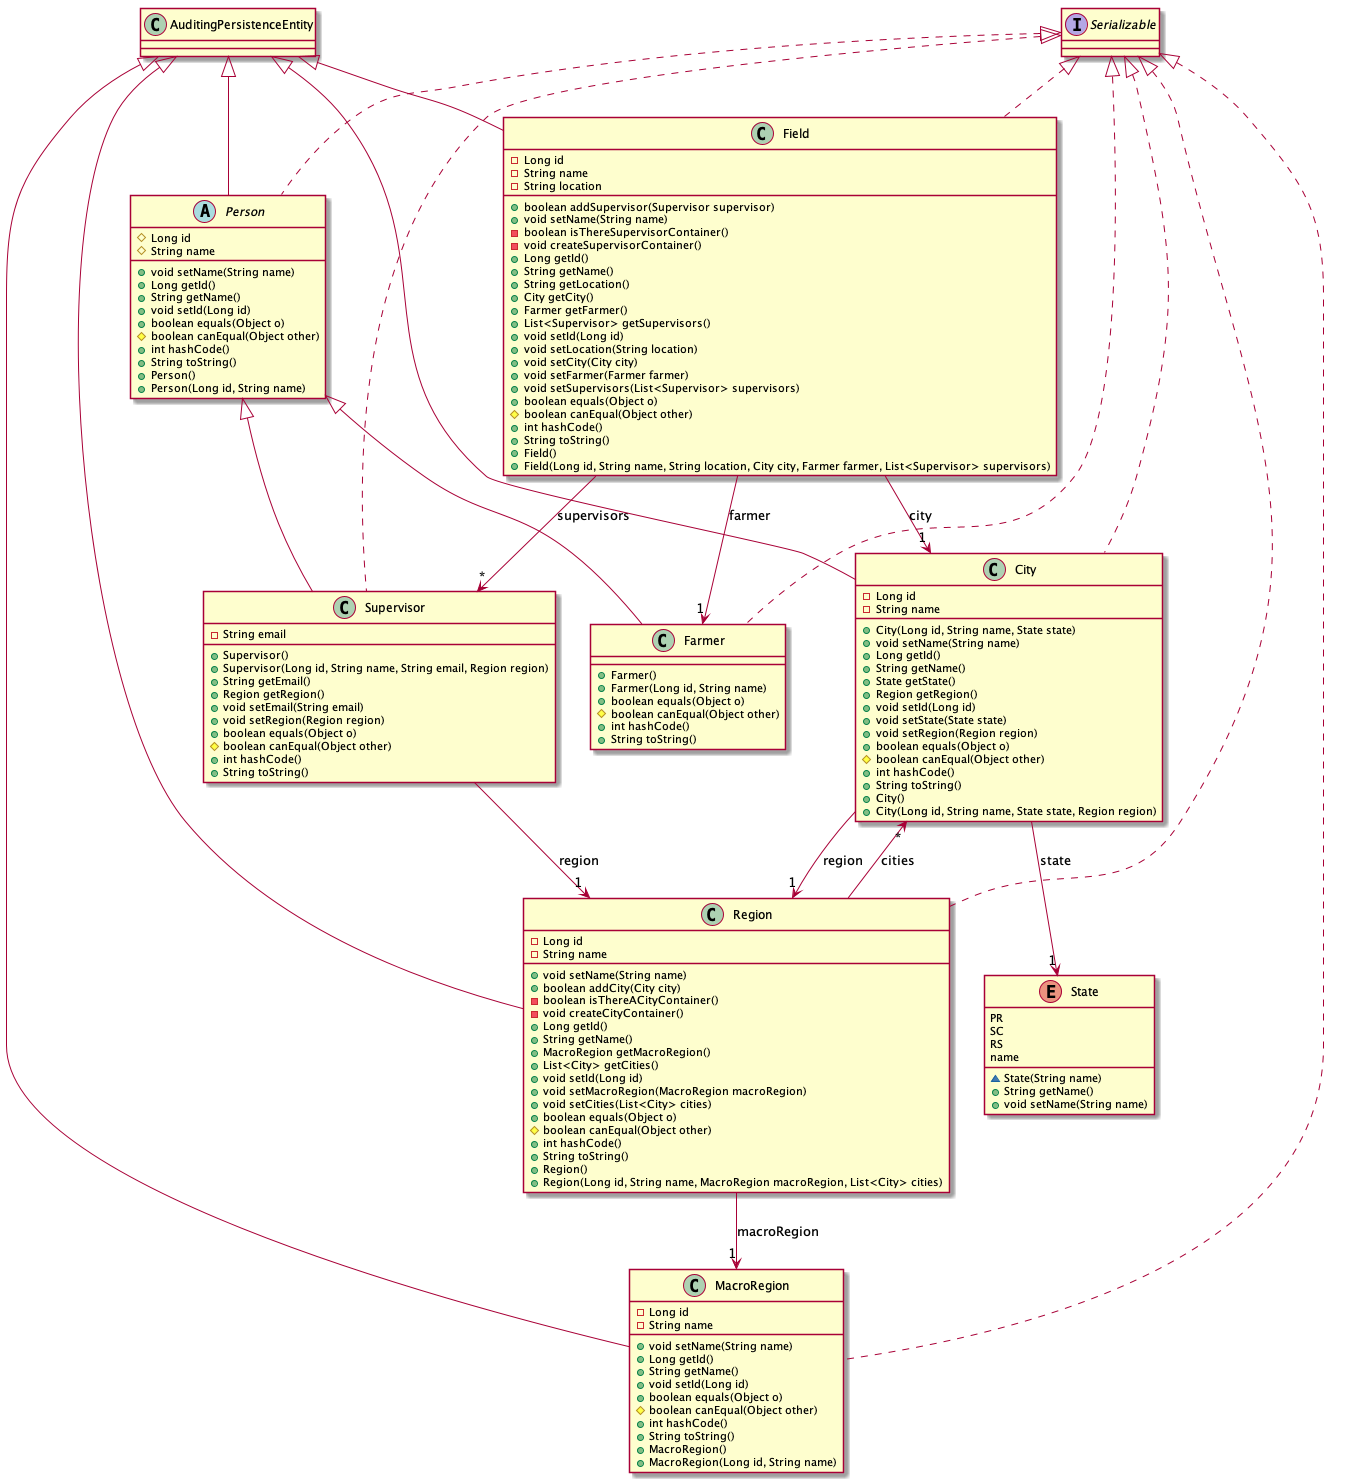
\includegraphics[scale=0.35]{dados/figuras/domain-base-classes.png}
	\caption{Diagrama de Classes Bases do Sistema.}
	FONTE: \cite[https:~//github.com/gabrielcostasilva/emater-mip-datacollection-app/tree/DDDLike/mip/src/main/resources/UMLDiagrams]{gabriel}
	\label{domain-base}
\end{figure}


\begin{landscape}
A FIGURA \ref{domain-survey} representa as classes relacionadas ao domínio das funcionalidades de pesquisa. No contexto da engenharia de software domínio de um sistema representa um conjunto de sistemas ou áreas que se comportam de forma similar.

\begin{figure}[h!]
	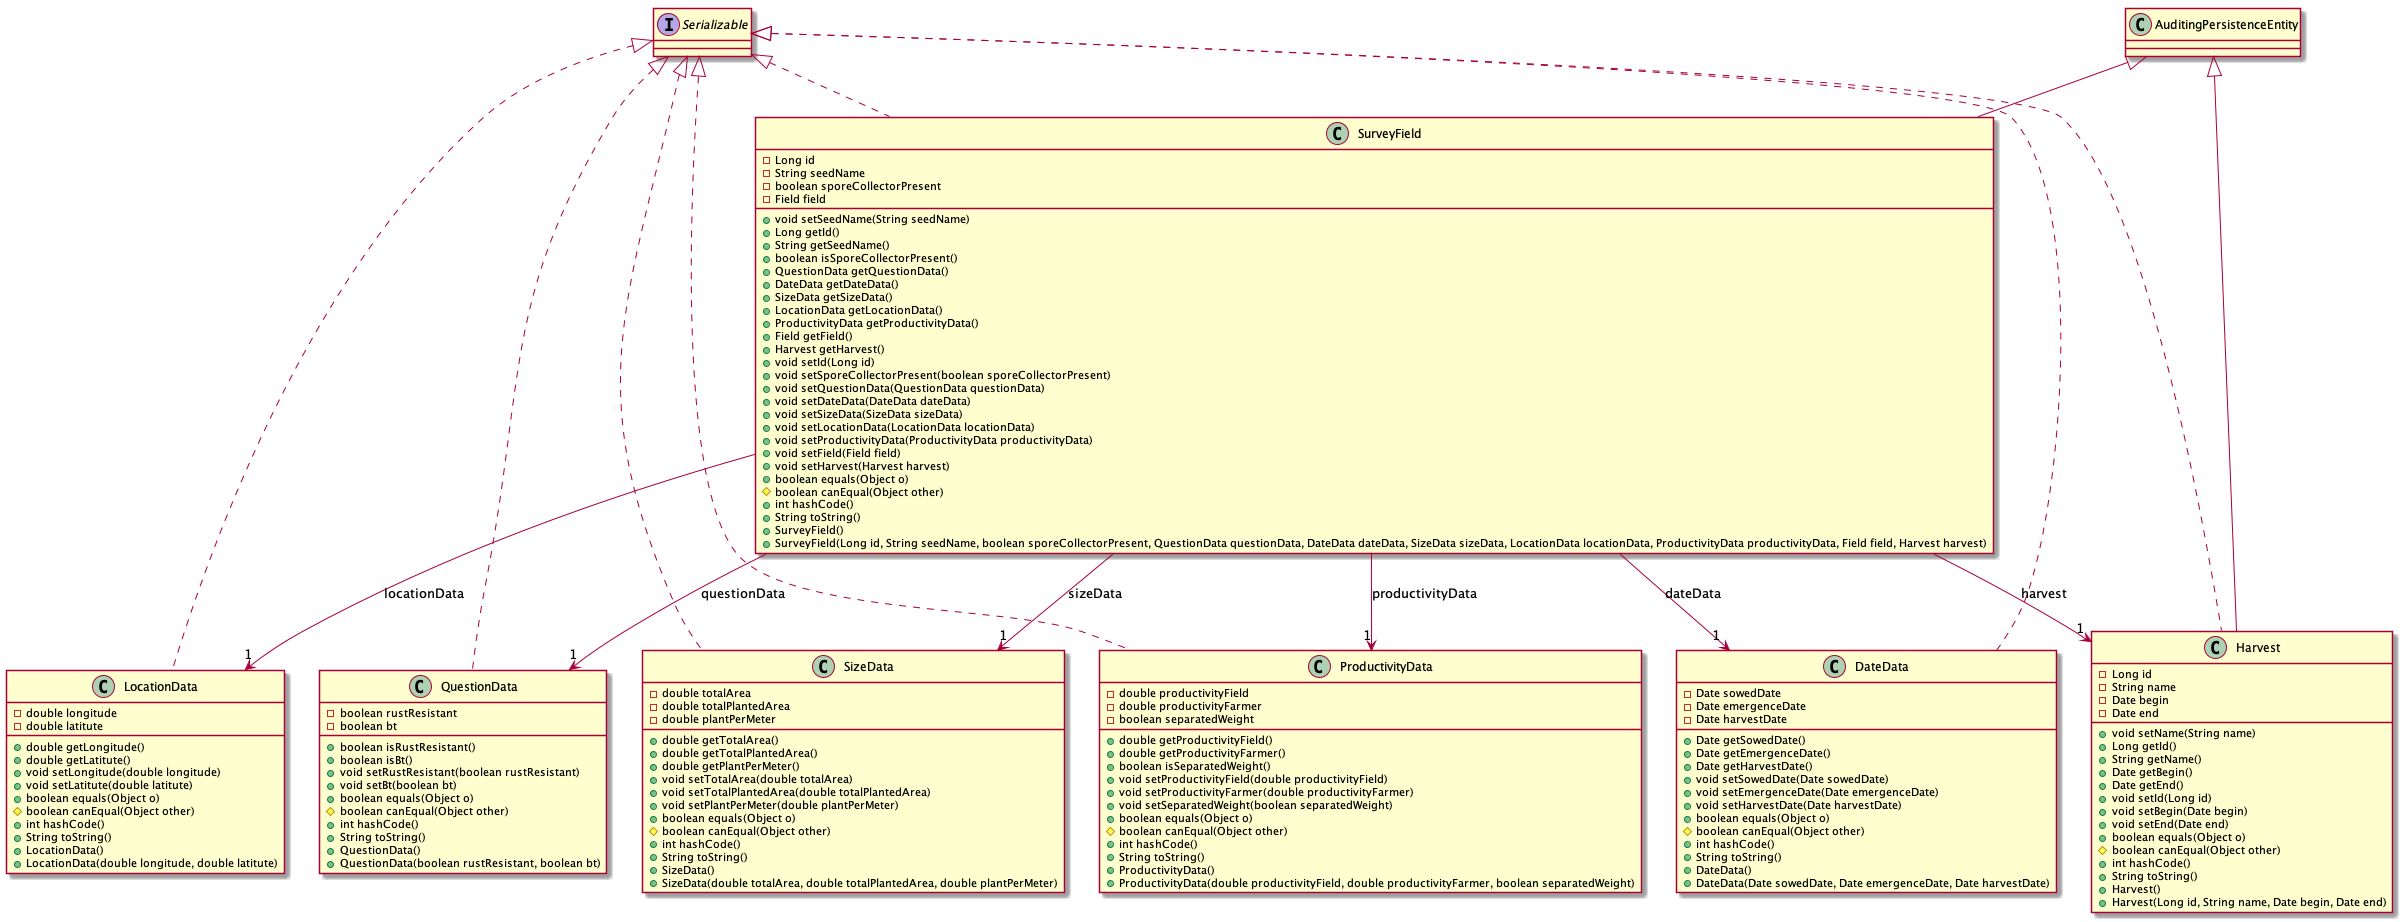
\includegraphics[scale=0.3]{dados/figuras/domain-survey-classes.png}
	\caption{Diagrama de Classes Domínio da Pesquisa.}
	FONTE: \cite[https:~//github.com/gabrielcostasilva/emater-mip-datacollection-app/tree/DDDLike/mip/src/main/resources/UMLDiagrams]{gabriel}
	\label{domain-survey}
\end{figure}
\end{landscape}



A FIGURA \ref{domain-pest} representa as classes relacionadas a coleta de dados sobre pragas. Funcionalidades de gerenciamento de pragas são apresentadas neste diagrama. 

\begin{figure}[h!]
	\centering
	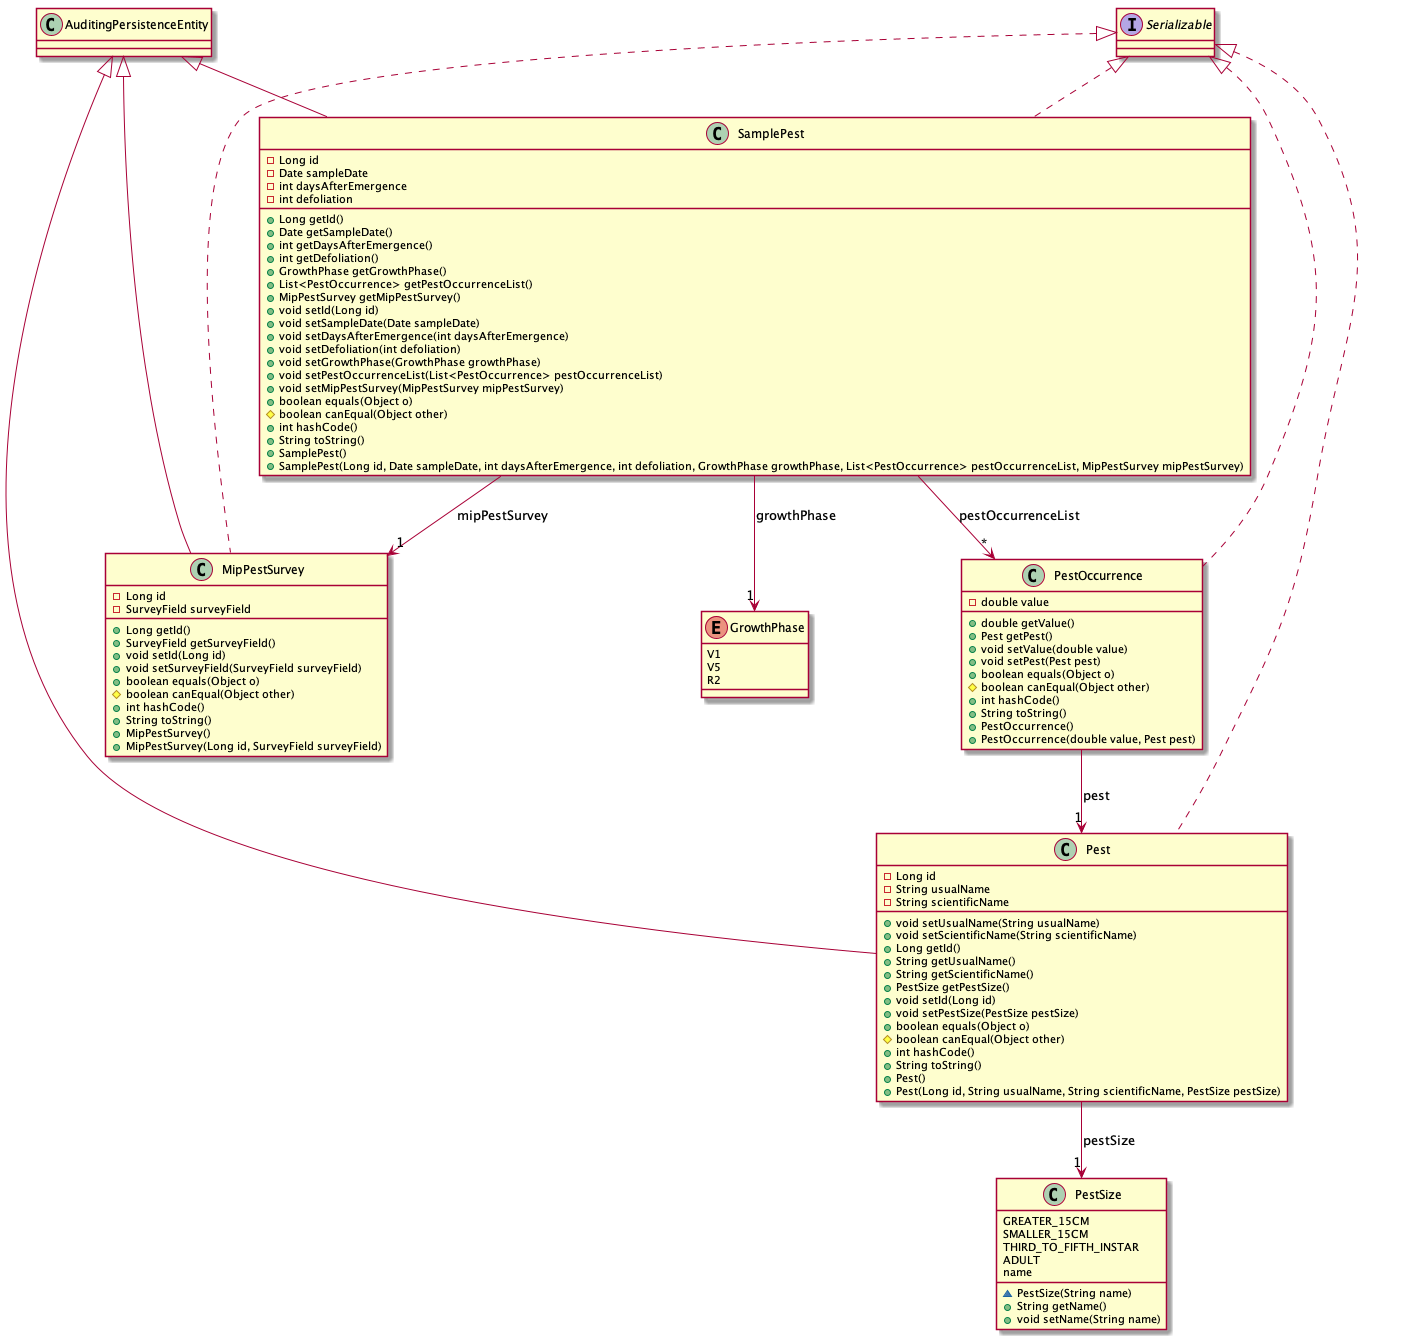
\includegraphics[scale=0.35]{dados/figuras/domain-mip-classes.png}
	\caption{Diagrama de Classes Gerenciamento de Pragas.} 
	FONTE: \cite[https:~//github.com/gabrielcostasilva/emater-mip-datacollection-app/tree/DDDLike/mip/src/main/resources/UMLDiagrams]{gabriel}
	\label{domain-pest}
\end{figure}



\section{TECNOLOGIA JAVA}

O Java é uma linguagem de programação e plataforma computacional orientada a objetos lançada pela primeira vez pela Sun Microsystems em 1995 e posteriormente adquirida pela ORACLE. Diferente das linguagens de programação convencionais, que são compiladas para código nativo o Java é compilada para um \textit{bytecode}\footnote{Conjunto de instruções projetada para execução eficiente por um interpretador de software. } que é interpretado por uma JVM \cite{Java}. A linguagem Java foi projetada para possuir portabilidade independente de plataforma, e segurança de rede, implementando restrições de execução.

\section{FERRAMENTAS}

A seguir, as ferramentas que serão utilizados no desenvolvimento dos
testes do sistema.

\subsection{JUnit}

O  \textit{JUnit} é um \textit{framework} para plataforma Java que possibilita a criação de classes de teste unitário. Por se tratar de uma ferramenta bastante difundida possui integração com diversas plataformas e IDEs. Além de tudo, ele é um projeto \textit{opensource}\footnote{Software de código aberto produzido de forma pública e colaborativa ou liberado sob uma licença na qual o detentor dos direitos autorais concede aos usuários os direitos para estudar, alterar e distribuir o software.} e permite que os testes sejam automatizados com apresentação de resultados. Os testes podem ser elaborados a partir dos requisitos do sistema ou casos de uso. 


Mais informações podem ser encontradas no capítulo 2 deste trabalho.

\subsection{Mockito}

O Mockito é um \textit{framework} de código aberto orientado a comportamento. Ele possibilita a simulação de comportamento de classes e interfaces facilitando a criação de testes que dependem de funcionalidades que ainda não foram implementadas. A ferramenta é bem difundida e possui integração com diferentes plataformas e IDEs. 

Mais informações podem ser encontradas no capítulo 2 deste trabalho.

\subsection{Spring Boot Test}

 Spring é um framework de código aberto, criado por Rod Johnson e possui o módulo de inicialização rápida. Spring Boot que é um projeto para facilitar o processo de configuração e publicação de aplicações \cite{spring}. O \textit{Spring Boot Test}  fornece suporte a testes de integração de forma fácil e simples. Através de anotações que o \textit{framework} disponibiliza é possível inicializar uma interface de conexão com o banco de dados permitindo a realização de testes de persistência e recuperação de dados.


Mais informações podem ser encontradas no capítulo 2 deste trabalho.

\subsection{IntelliJ IDEA}

O ambiente de desenvolvimento integrado IntelliJ IDEA, desenvolvido pela JetBrains é um programa  para desenvolvimento de \textit{software} em várias linguagens que suporta várias tecnologias e \textit{frameworks}. O Intellij possui um decompilador\footnote{Realiza a operação inversa de um compilador, transformando código objeto em código fonte.}, que permite debugar\footnote{Método para procurar um erro em um trecho de código.} o código interno de classes desenvolvidas e códigos externo de bibliotecas que não possuem fonte. Ele também conta com recursos de conexão a banco de dados o que permitem criar, alterar e excluir registros. Além de contar com a pesquisa rápida que permite a visualização e previsão de resultados, facilitando a interação com classes, bibliotecas e \textit{frameworks} \cite{intellij}.


\section{MÉTODO}

O sistema de Manejo Integrado de Pragas e Doenças deverá ser submetido a testes de unidade e integração. Os testes de unidade avaliarão isoladamente o banco de dados, as interfaces de comunicação, e todos os outros componentes do projeto. Os testes de integração testarão os componentes, previamente testados isoladamente, acoplados. O objetivo é identificar possíveis falhas nos acoplamentos. 


O processo de teste deve se basear em uma metodologia compatível com o processo de desenvolvimento e deve ser o guia básico para organizar a atividade de teste da aplicação. 


\subsection{Modelo 3P x 3E}

O modelo proposto é composto por diversas fases e etapas sendo duas em paralelo e quatro em sequência. As etapas em paralelo representam a preparação e o planejamento que devem estar presentes no projeto des de sua concepção e fornece suporte para as demais etapas do processo. Procedimentos iniciais representam a menor parte do processo, a maior parte do processo deve se dedicar as etapas de especificação, execução e entrega \cite{riosMoreira}. A FIGURA \ref{modelo3p3e} apresenta o modelo.


\begin{figure}[H]
	\centering
	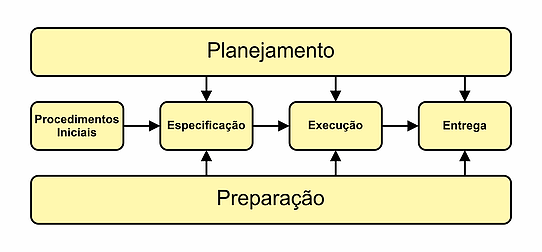
\includegraphics[scale=3.5]{dados/figuras/modelo3px3e.png}
	\caption{Modelo 3P x 3E do ciclo de vida do processo de teste.}FONTE: \cite{riosMoreira}
	\label{modelo3p3e}
\end{figure}



A primeira etapa “Procedimentos iniciais” propõe a análise e verificação dos requisitos para garantir que estes estejam completos e sem ambiguidades. Além disso o procedimento inicial deve conter as atividades que serão executadas ao longo de todo o desenvolvimento dos testes.


A segunda etapa de “Especificação” consiste em elaboração de casos de teste e elaboração de roteiros de teste. Deve-se retornar a esta etapa quando necessário pois novos requisitos podem surgir ou se alterarem.

A terceira etapa de “execução” se refere a etapa anterior de “Especificação”, os casos e roteiros de testes devem ser executados e seus resultados encontrados devem ser relatados.


 A quarta etapa “Entrega” se refere a finalização do processo de teste onde serão entregues os resultados obtidos e os artefatos gerados durante todo o processo.
 
 
As etapas de “Planejamento e Preparação” se dão ao longo de todo o projeto e são utilizadas de apoio, a preparação é basicamente responsável por preparar todo o ambiente de teste para que não haja obstáculos durante a execução, o planejamento é a atividade que permanece ativa durante todo o projeto para evitar desvios do objetivo principal.

\section{VALIDAÇÃO DO PROJETO}

% Esse é um teste\footnote{Esse é o exemplo de nota de rodaé.}.

Esta atividade se resume em avaliar se os artefatos entregues atendem com eficiência as metas propostas, além de apontar possíveis melhorias. Para cada requisito do sistema deve ser possível produzir um ou mais casos de testes de caixa-preta para verificar se o sistema cumpre o que foi projetado para fazer. Os testes definidos devem possuir um roteiro bem estruturado para validação do requisito, se não for possível a criação de um teste para um requisito será necessária uma melhor especificação deste requisito. Após os testes especificados estes serão executados por desenvolvedores e usuários para a validação do sistema. Ao final os testadores devem responder a um questionário fechado com perguntas pré-definidas. A partir do resultado do questionário serão levantados os pontos positivos e negativos do sistema, e possíveis melhorias podem ser acatadas.                   % Metodologia
% 
\chapter{RESULTADOS}

Este capitulo expõe os resultados obtidos através da execução dos testes de unidade no aplicativo MIP, como o número de testes desenvolvidos durante o desenvolvimento do trabalho é extenso foram escolhidas as principais classes do pacote \textit{Entity} (\textit{Field.java e Survey.java}), e as principais classes do pacote \textit{Service} (\textit{FieldService.java e SurveyService.java}). para serem analisadas profundamente. 


\section{APURAÇÃO DOS TESTES PACOTE ENTITY}

O pacote \textit{Entity} é responsável por armazenar as classes que realizam o mapeamento objeto-relacional, e nele é definida as principais regras de negócio do sistema. O pacote é composto por 5 sub pacotes sendo eles: 

\begin{itemize}

\item[1]Pacote \textit{base}: Armazenas as classes que define a estrutura básica do sistema, as classes que definem regiões (\textit{Region.java}), cidades (\textit{City.java}), estados (\textit{State.java}) e macrorregiões (\textit{MacroRegion.java}), assim como as que definem supervisores (\textit{Supervisor.java}) e agricultor (\textit{Farmer.java}). Todos esses dados compõem um registro (\textit{Field.java}) que estabelece uma ligação entre localização, supervisores e agricultor. Além disso o pacote contém mais duas superclasses, \textit{AuditingPersistenceEntity.java} responsável por armazenar metadados dos objetos, e \textit{Person.java} responsável por definir os atributos básicos de uma pessoa.  

\item[2]Pacote mid: Armazena as classes que definem a estrutura básica para coleta e análise de esporos de ferrugem asiática e doenças que afetam a lavoura. A classe \textit{AsiaticRustTypesLeafInspection.java} contém os tipos de lesões causadas pela ferrugem em plantas, a classe \textit{AsiaticRustTypesSporeCollector.java} contém os tipos de análise que podem ser retiradas do coletor de esporos, a classe \textit{BladeReadingResponsibleEntity.java} armazena a entidade responsável pela leitura de laminas de esporos, classe \textit{BladeReadingResponsiblePerson.java} é responsável por armazenar a pessoa responsável pela leitura de esporos, \textit{MIDSampleSporeCollectorOccurrence.java} trata os dados da amostra de esporos coletada, \textit{MIDSampleLeafInspectionOccurrence.java} trata os dados da inspeção das folhas coletada, \textit{MIDSampleFungicideApplicationOccurrence.java} trata os dados da aplicação de fungicida contra a ferrugem. A classe principal deste pacote é a \textit{MIDRustSample.java} pois é nela onde são armazenados todos os registros de aplicação de fungicida, de coleta de folhas, de coleta de sopros e os responsáveis pelas análises. 

\item[3]Pacote mip: Armazena as classes que definem a estrutura básica para coleta e análise de pragas que atingem a lavoura.  A classe \textit{Pest.java} registra os tipos de pragas que podem atingir uma lavoura, \textit{PestDisease.java} armazena as doenças causadas por pragas, \textit{PestSize.java} é responsável pelo armazenamento do tamanho das pragas. \textit{GrowthPhase.java} registra a fase de crescimento em que a praga foi encontrada, \textit{PestNaturalPredator.java} armazena os predadores naturais das pragas, \textit{MIPSamplePestOccurrence.java} registra a ocorrência de pragas em uma lavoura, \textit{MIPSamplePestDiseaseOccurrence.java} registra a ocorrência de doenças causadas por pragas em uma lavoura, \textit{MIPSampleNaturalPredatorOccurrence.java} registra a ocorrência de predadores naturais na lavoura. A classe principal deste pacote é a \textit{MIPSample.java} ela é responsável por armazenar os dados de pragas, doenças causadas por pragas e predadores naturais que atingem uma lavoura.

\item[4]Pacote \textit{pulverisation}: Armazena as classes que definem a estrutura básica para a atividade de pulverização de uma lavoura. As classes \textit{ProductUnit.java} e \textit{Product.java} são responsáveis por tratar dos produtos que serão utilizados durante a pulverização, definem unidade de medida do produto e características do produto como nome e dose respectivamente. As classes \textit{TargetCategory.java} e \textit{Target.java} definem a categoria alvo do pesticida e qual praga ele combate respectivamente. A classe \textit{PulverisationOperationOccurrence.java} define uma ocorrência de pulverização.  A principal classe deste pacote é a \textit{PulverisationOperation.java} esta contém os dados referente a todas as pulverizações que foram realizadas. 

\item[5]Pacote \textit{survey}: Armazena as classes que definem a estrutura básica para realizar uma pesquisa de campo através dos dados coletados com o manejo integrado de pragas e com o manejo integrado de doenças. A classe \textit{DateData.java} armazena os dados de uma colheita como data de semeadura e data da colheita, a classe \textit{SizeData.java} contém os dados referente a área da colheita, a classe \textit{LocationData.java} contém dados referente a localização da colheita, a classe \textit{ProductivityData.java} contém dados referente a produtividade de uma colheita, a classe \textit{QuestionData.java} registra dados específicos referente a plantação, se a plantação é resistente a ferrugem por exemplo, a classe \textit{Harvest.java} e responsável por registrar dados referente a colheita como o início e o fim da colheita. A principal classe deste pacote é a \textit{Survey.java} ela é responsável por armazenar todos os dados referente a uma pesquisa da produção da lavoura de um produtor.

\end{itemize}{}

\subsection{RESULTADO DOS TESTES CLASSE FIELD.JAVA}

Como já foi ressaltado anteriormente uma das principais classes do sistema é a \textit{Field.java}, a FIGURA \ref{diagrmaTestField} apresenta o diagrama de classes que expressa a classe \textit{Field.java}, e as demais classes que a compõem assim como a classe responsável por testá-la, a classe FieldTest.java. Também é possível analisar no diagrama os atributos e métodos que pertence à classe \textit{Field}, assim como os métodos e atributos da classe de teste \textit{FieldTest}.

\begin{figure}[H]
	\centering
	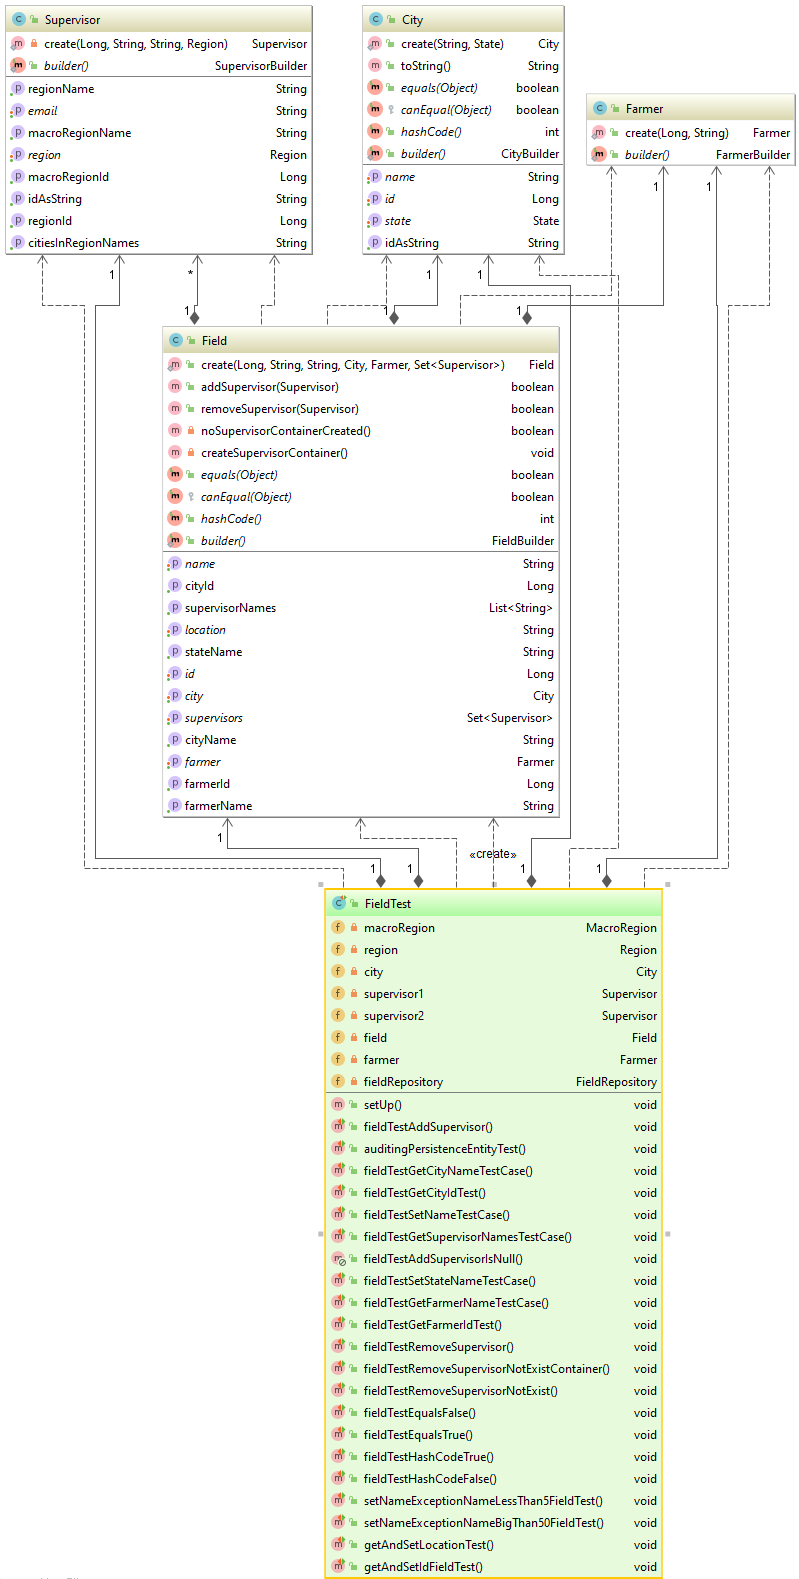
\includegraphics[scale=0.58]{dados/figuras/PackagebaseTestField.png}
	\caption{Diagram de Classes Field e FieldTest.}
	\label{diagrmaTestField}
\end{figure}

A classe de teste apresentada na FIGURA \ref{diagrmaTestField} possui vinte e um métodos de teste e um método de apoio aos testes denominado \textit{“setUp”}, o objetivo dos testes é exercitar a classe \textit{Field} até que todos as variáveis, entradas e saídas de dados sejam executados pelo menos uma vez. Como a classe \textit{Field} é composta por outras classes se faz necessário a instanciação de outras classes como \textit{Supervisor}, \textit{Farmer}, \textit{City} e outras para a execução completa dos testes. Como a classe se trata de uma entidade que será persistida em um banco de dados, ela possui certas regras de negócio que serão ativadas somente no momento de gravar os dados no banco, sendo assim foi preciso criar uma referência para a interface \textit{FieldRepository}, classe responsável por realizar a persistência dos dados no banco. Como o objetivo deste trabalho é cobrir o sistema com testes unitários e testes que integram classes entidades com o banco de dados ou comunicação com \textit{APIs} são testes de integração foi utilizado um\textit{ “Mock”} para simular o comportamento do repositório.

A FIGURA \ref{field1} apresenta a declaração da classe de testes, os atributos utilizados para desenvolver os testes e o método\textit{ “setUp”} utilizado para preparar o ambiente para os testes.


O trecho de código da FIGURA \ref{field1} apresenta as seguintes funcionalidades:





\begin{itemize}

\item Na linha 1 é utilizada a anotação \textit{@SpringBootTest} que prepara um contexto \textit{Spring} e inclui a possibilidade de iniciar um container em um porta default ou configurada pelo usuário. O que não é necessário para o tipo de teste executado nesta classe; 

 \item Na linha 2 é utilizada a anotação \textit{@FixMethodOrder} que permite definir uma ordem de execução dos testes, neste casso foi definida a ordem \textit{“NAME\_ASCENDING"} que faz a execução dos testes de acordo com o nome de maneira ascendente;

 \item Linha 3 a classe \textit{FieldTest} é aberta;

 \item Da linha 5 a 10 há a declaração dos objetos que serão utilizadas nos testes;
 
  \item Na linha 12 um objeto do tipo \textit{FieldRepositorio} e declarado e instanciado como um objeto \textit{mock}.

 \item Na linha 15 é utilizado a anotação \textit{@Before}, esta anotação determina que, sempre antes da execução de um teste o método \textit{“setUp”} deve ser executado primeiro.

 \item O método \textit{“setUp”} que tem sua declaração na linha 15 e vai até a linha 30 é responsável por realizar a construção dos objetos declarados nas linhas 5 a 10.


\end{itemize}{}



A FIGURA \ref{field1} apresenta os casos de testes criados para a classe \textit{Field}. 


A ideia geral na elaboração dos testes é a de cobrir cada atribuição de dados, as entrada e saída de dados da classe \textit{Field}, buscando a cobertura de 100\% das linhas métodos e atributo da classe. Os resultados obtidos da execução dos testes foram listados a seguir:

Método de teste \textit{“fieldTestAddSupervisor()”} linhas 32 a 36 figura \ref{field1}: Este método é responsável por testar se um objeto do tipo\textit{ “supervisor”} é adicionado ao objeto testado através do método de entrada \textit{“field.addSupervisor(Supervisor supervisor)”}.  Neste teste a entrada é um objeto do tipo \textit{“Supervisor” }e a saída do método é uma variável do tipo \textit{“boolean”}(verdadeiro ou falso).  As entradas foram criadas nas linhas 24 e 26 e fornecidas como entradas ao método testado nas linhas 34 e 35 respectivamente. A saída é um \textit{“TRUE”} já que os objetos passados são adicionados a classe\textit{ “Field”}. 



Método de teste\textit{ “auditingPersistenceEntityTest()”} linhas 38 a 47 figura \ref{field1}: Este método é responsável por testar os atributos criados na superclasse\textit{ “auditingPersistenceEntity”}, como uma superclasse não pode ser testada os métodos e atributos dela devem ser testados em uma das subclasses.  A classe é composta por dois atributos do tipo \textit{long “LastModified”} e \textit{“CreatedAt”,} O objetivo deste teste é de atribuir valor as variáveis e verificar se os valores atribuídos são recuperados corretamente. As entradas foram criadas nas linhas 40 e 41 e atribuídas ao objeto testado nas linhas 43 e 44 respectivamente. Posteriormente nas linhas 45 e 46 é feita a confirmação das saídas contendo os valores 11 e 12 do tipo \textit{“long”.}

Método de teste \textit{“fieldTestGetCityNameTestCase ()”} linhas 49 a 52 figura \ref{field1}: Este caso de teste verifica se um nome atribuído a uma cidade é recuperado pelo método \textit{“field.getCityName()”.} A entrada é uma \textit{String} de caracteres, e a saída deve ser uma \textit{String} de caracteres formatados com a primeira letra de cada palavra maiúscula.  O objeto do tipo \textit{“city” }é criado na linha 19 o atribuído nome é definido como “NOvA FAtimA” em seguida o objeto\textit{ “city”} é atribuído ao objeto\textit{ “Field” }na linha 28 /29. Já no teste o valor e recuperado é o retorno é “Nova Fatima”.


\begin{figure}[H]
	\centering  
	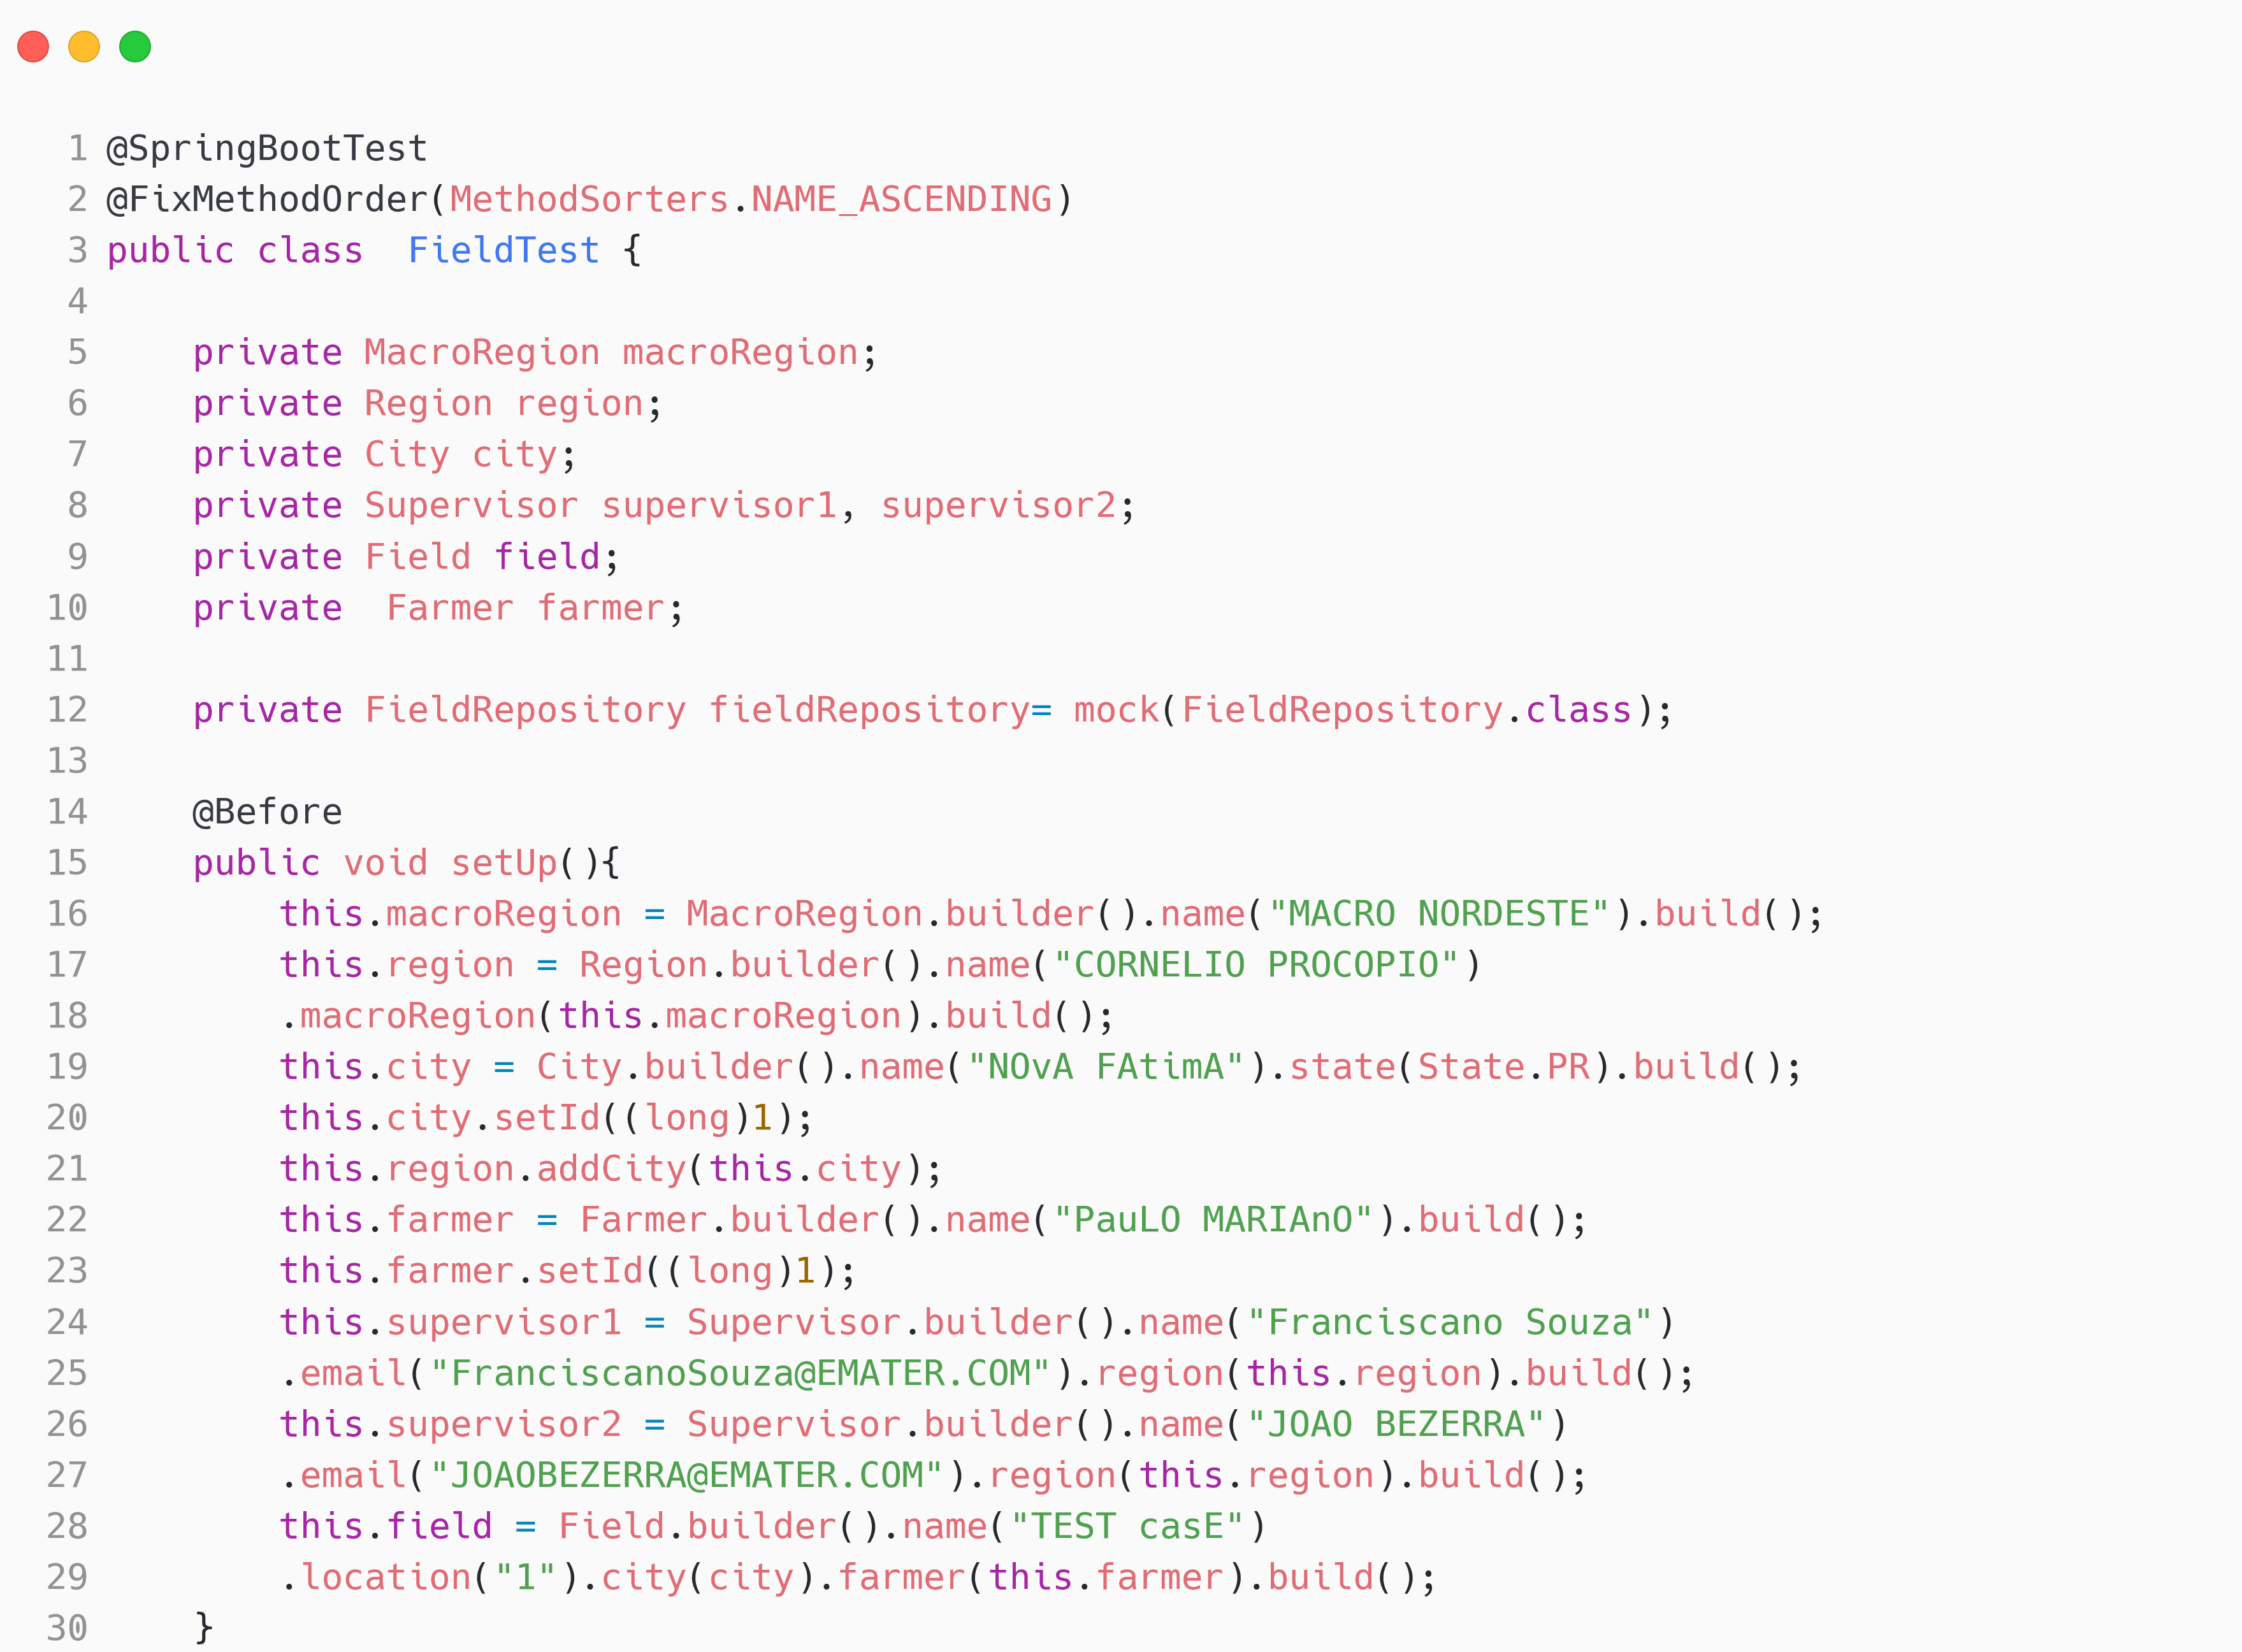
\includegraphics[scale=0.18]{dados/figuras/buildTestField.png}
\end{figure}

\begin{figure}[H]
	\centering
	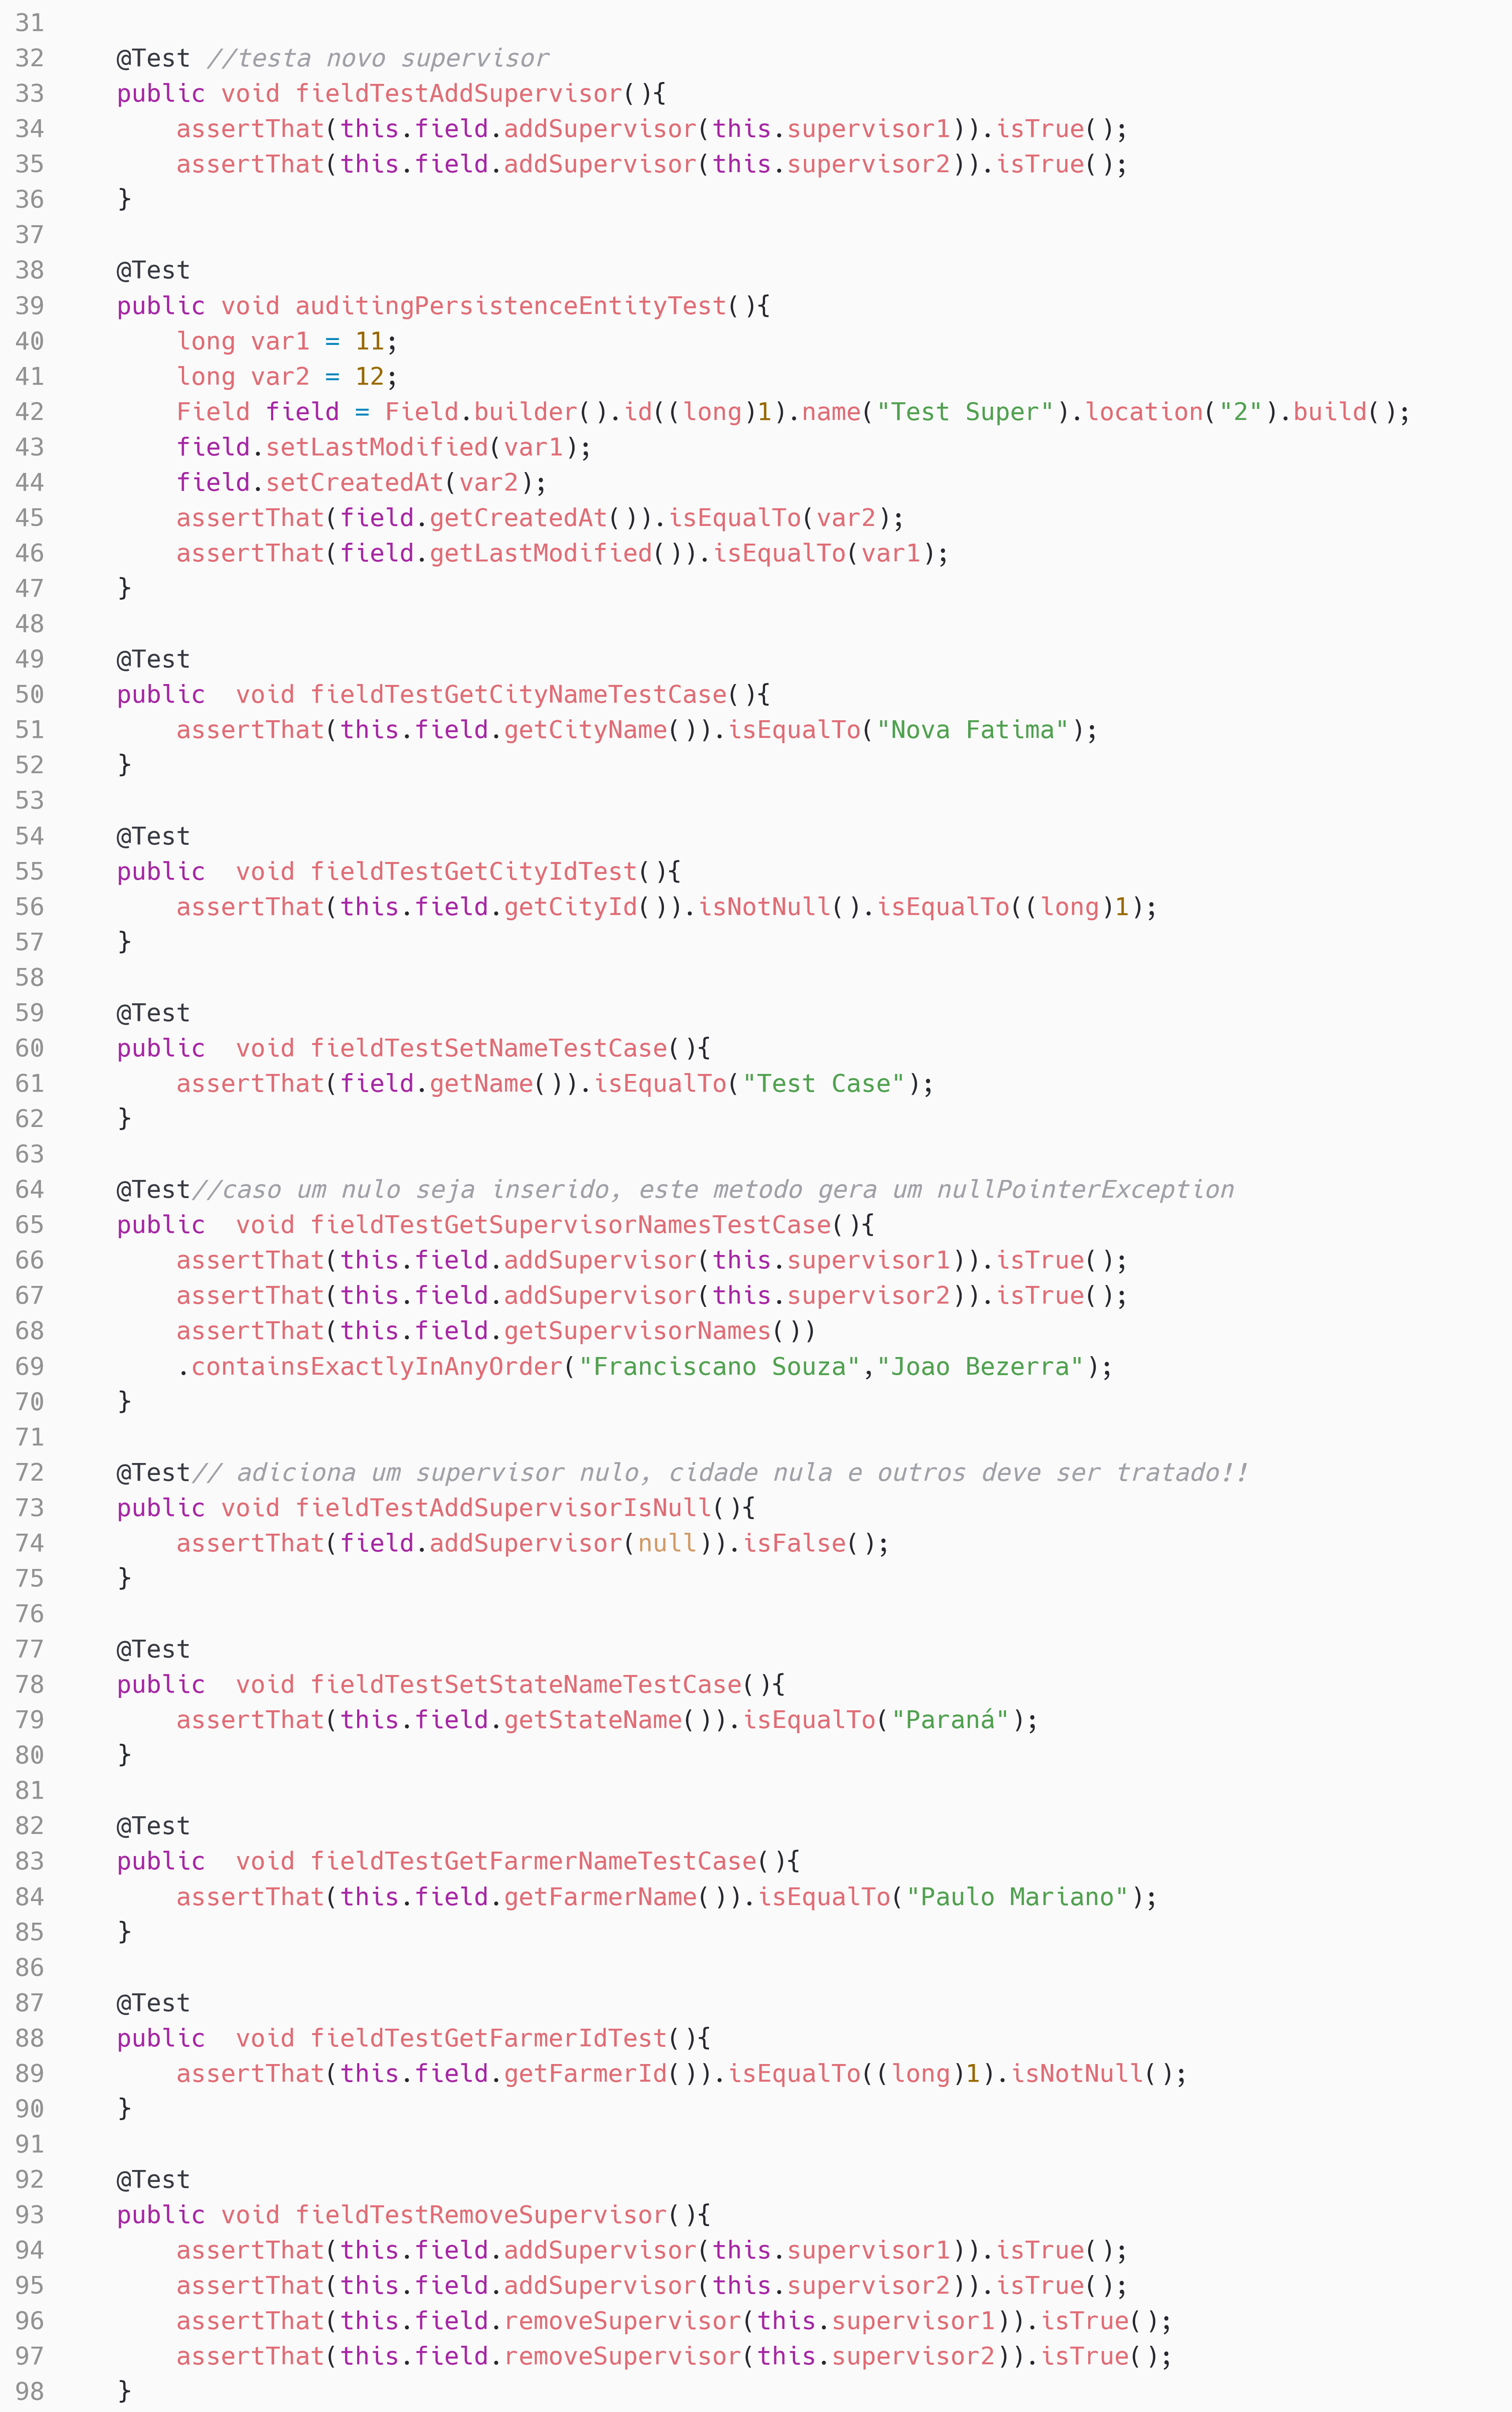
\includegraphics[scale=0.18]{dados/figuras/carbonField1.png}
\end{figure}

\begin{figure}[H]
	\centering
	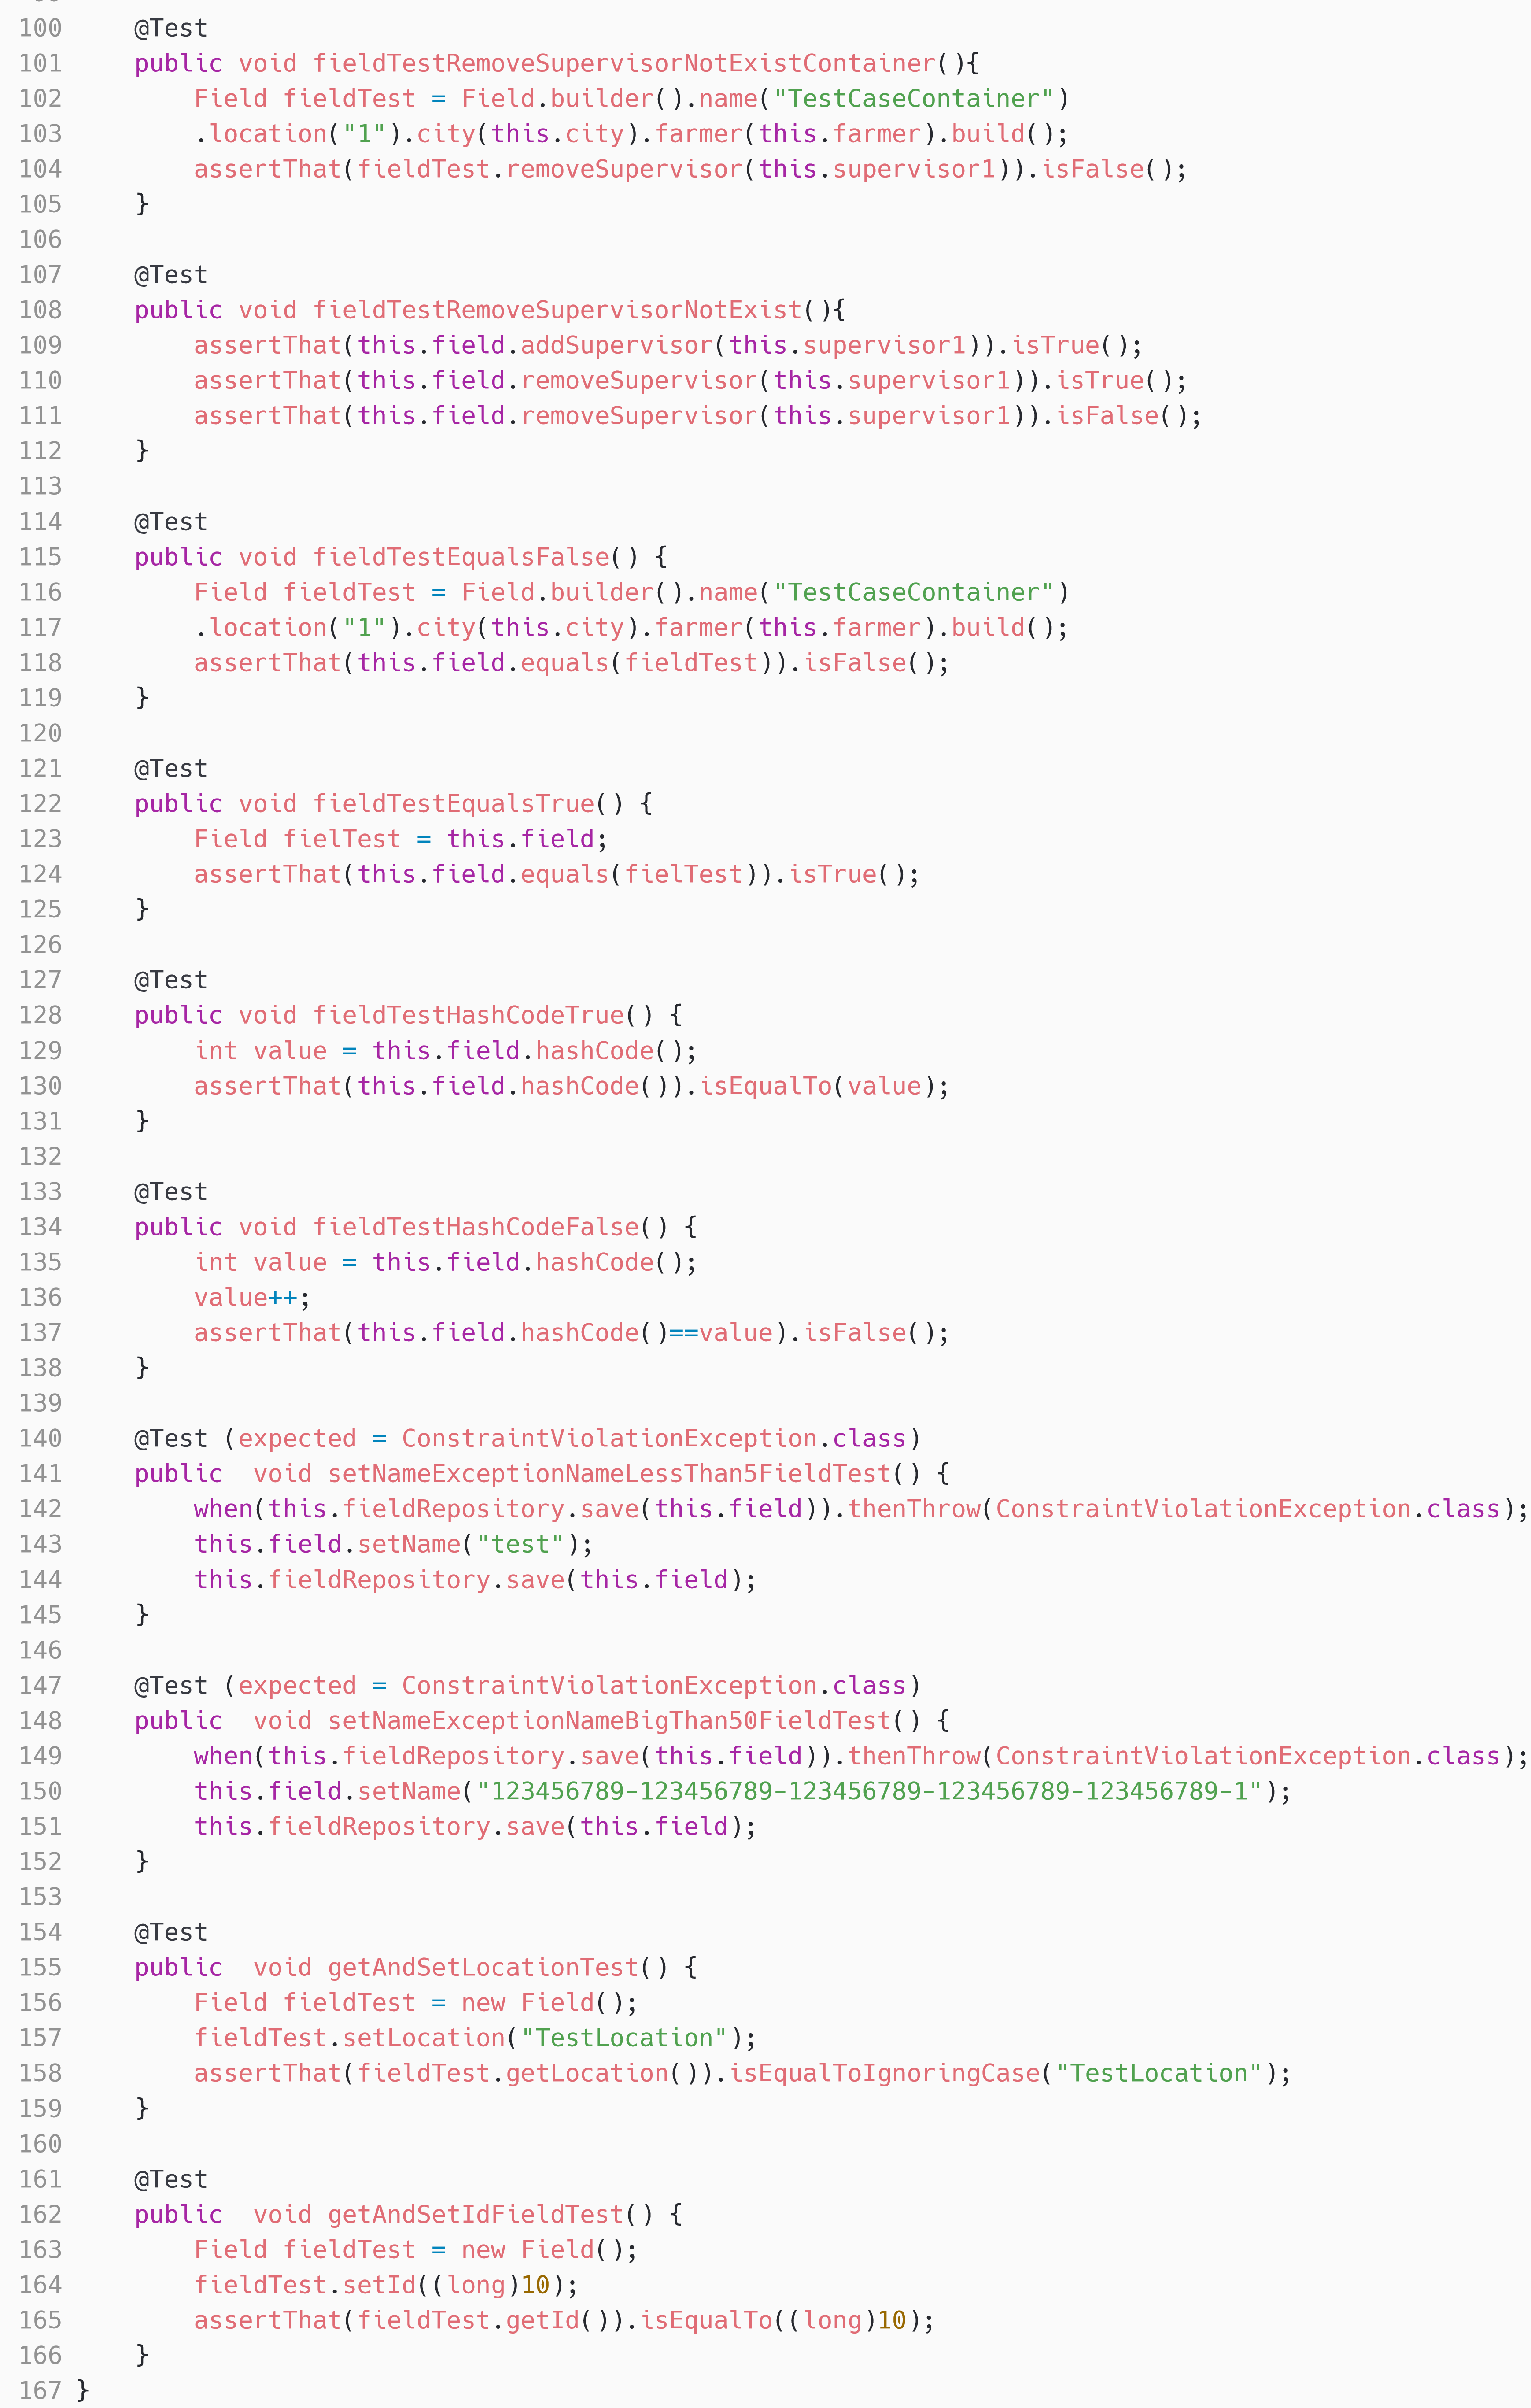
\includegraphics[scale=0.17]{dados/figuras/carbonField2.png}
	\caption{Classe de teste FieldTest.java.}
	\label{field1}
\end{figure}






Método de teste\textit{ “fieldTestGetSupervisorNamesTestCase()”} linhas 64 a 70 figura \ref{field1}: Este caso de teste verifica se o método\textit{ “Field.getSupervisorNames ()”} recupera os nomes de todos os supervisores adicionados ao objeto \textit{“Field”.} Os supervisores são criados nas linhas 24 a 27 e são adicionados a\textit{ “Field”} nas linhas 66 e 67. A entrada é composta por dois supervisores de nomes diferentes ("Franciscano Souza" e "Joao Bezerra"). O retorno do método testado consiste em uma lista do tipo \textit{“String”}, o teste verifica se a lista contem em qualquer ordem os elementos os elementos inseridos, o retorno é ("Franciscano Souza" e "Joao Bezerra");

Método de teste\textit{ “fieldTestAddSupervisorIsNull()”} linhas 72 a 75 figura \ref{field1}: Este caso de teste consiste em inserir um supervisor como\textit{ “null”}, caso o nulo seja inserido gera uma inconsistência pois outros métodos de consulta podem falhar. A entrada é um\textit{ “null”} linha 74, e o retorno esperado é um \textit{“FALSE”,} pois, a inserção não deve ser realizada, mas o retorno é um\textit{ “TRUE”} confirmando à inserção de um nulo como um supervisor. Esta inserção pode gerar uma inconsistência em consultas futuras.

Método de teste\textit{ “fieldTestSetStateNameTestCase ()”} linhas 64 a 70 figura \ref{field1}: Este teste consiste em recuperar o nome do estado a qual a cidade pertence. A Entrada consiste em um objeto do tipo \textit{“Estate.PR”} linha 19. O retorno esperado é uma \textit{string} de caracteres contendo “Paraná”. O retorno do método testado é uma \textit{string} contendo “Paraná”   

Método de teste \textit{“fieldTestGetFarmerNameTestCase ()”} linhas 82 a 85 figura \ref{field1}: Este meto busca o nome do agricultor atribuído ao objeto\textit{ “Field”}. A entrada consiste em um objeto do tipo\textit{ “Farme” }com o atributo nome definido como “PauLO MARIAnO” linha 22. O retorno do método testado deve ser uma \textit{string} contendo o nome do agricultor formatado com a primeira letra de cada palavra maiúscula. O retorno do teste linha 84 é uma \textit{string} que contem “Paulo Mariano”.


Método de teste\textit{ “fieldTestGetFarmerIdTest ()”} linhas 87 a 90 figura \ref{field1}: Este método consiste em recuperar o atribuo identificador de agricultor a entrada é feita na linha 23 sendo o valor (\textit{long} 1). O retorno do método testado deve ser um \textit{long} contendo o identificador único do agricultor. O retorno do meto é um tipo \textit{long} contendo o valor 1. 


Método de teste \textit{“fieldTestRemoveSupervisor ()”} linhas 92 a 98 figura \ref{field1}: Este teste consiste em atribuir novos supervisores a um objeto\textit{ “Field”} e em seguida remove-los. A entrada consiste em dois supervisores linhas 94 e 95. A saída consiste em um\textit{ “boolean”} para cada remoção\textit{, “TRUE”} caso o supervisor seja removido, e\textit{ “FALSE”} caso o supervisor não seja removido.  A sida nesse teste é\textit{ “TRUE”} para as duas execuções pois os dois supervisores enviados para remoção foram encontrados.

Método de teste\textit{ “fieldTestRemoveSupervisorNotExistContainer ()”} linhas 100 a 105 figura \ref{field1}: Este caso de teste consiste em tentar remover um supervisor de um objeto \textit{“Field” }sem que não haja um container do tipo supervisor criado em\textit{ “Field”}. A entrada consiste em um supervisor não pertencente ao objeto \textit{“FieldTest”} criado na linha 102. A saída nesse caso de teste é um\textit{ “FALSE”} pois ainda não foi inserido nenhum supervisor a \textit{“FieldTest”}.
 
Método de teste \textit{“fieldTestRemoveSupervisorNotExist()” }linhas 107 a 112 figura \ref{field1}: Este método consiste em testar a remoção de um supervisor que já foi removido anteriormente. A entrada consiste em um supervisor linhas 109. A saída consiste em \textit{“TRUE”} caso os objetos sejam removidos com sucesso, saída apresentada na linha 110 ou \textit{“FALSE”} caso o supervisor já não exista mais em\textit{ “Field” }saída apresentada na linha 111.

Método de teste\textit{ “fieldTestEqualsFalse()”} linhas 114 a 119 figura \ref{field1}: Este método de teste consiste em comparar dois objetos do tipo\textit{ “Field”} caso eles sejam iguais o retorno é um\textit{ “boolean” “TRUE”} caso sejam diferentes o retorno é um\textit{ “FALSE”}. A entrada consiste em dois objetos do tipo\textit{ “Field”}, o primeiro objeto é criado nas linhas 28 e 29, o segundo objeto é criado nas linhas 116 e 117. A saída é um \textit{“FALSE” }pois os objetos comparados são diferentes.

Método de teste \textit{“fieldTestEqualsTrue()” }linhas 121 a 125 figura \ref{field1}: Este método de teste consiste em comparar dois objetos do tipo\textit{ “Field”} caso eles sejam iguais o retorno é um \textit{“boolean” “TRUE”} caso sejam diferentes o retorno é um\textit{ “FALSE”}. A entrada consiste em dois objetos do tipo \textit{“Field”,} o primeiro objeto é criado nas linhas 28 e 29, o segundo objeto é criado nas linhas 116 e 117 e recebe uma cópia do objeto criado anteriormente. A saída é um \textit{“TRUE” }pois os objetos são iguais.

Método de teste \textit{“fieldTestHashCodeTrue()” }linhas 127 a 131 figura \ref{field1}: Este teste consiste em recuperar o valor de \textit{“hashcode” }de um objeto e verifica seu valor em uma segunda chamada. O método não possui entrada. A saída consiste em um valor numérico do tipo \textit{“int”.} O valor de \textit{hash} é recuperado em uma primeira chamada na  linha 129. em seguida é feita uma assertiva, esta compara o valor recuperado anteriormente com o valor de uma nova chamda do método de \textit{hash}, os valores são iguais.

Método de teste\textit{ “fieldTestHashCodeFalse()”} linhas 133 a 138 figura \ref{field1}: Este teste consiste em recuperar o valor de\textit{ “hashcode”} de um objeto e verifica seu valor em uma segunda chamada. O método não possui entrada. A saída consiste em um valor numérico do tipo \textit{“int”.} O valor de \textit{hash} é recuperado em uma primeira chamada na linha 135, em seguida é feito um incremento no valor recuperado. Uma assertiva compara o valor chamado anteriormente e incrementado com o valor de uma nova chamda do método de \textit{hash}, os valores são diferentes..

Método de teste \textit{“setNameExceptionNameLessThan5FieldTest()”} linhas 140 a 145 figura \ref{field1}: Uma das restrições que se encontra na hora de salvar um objeto do tipo \textit{“Field” }é que a variável\textit{ “name”} do tipo \textit{“String” }deve ter entre 5 e 50 caracteres. A entrada consiste em uma\textit{ “String”} contendo apenas quatro caractere. A saída esperada é uma exceção de violação das regras do banco. A saída deste teste é uma \textit{“ConstraintViolationException.class” }disparada pelo\textit{ “FieldRepository.class”} pois o valor atribuído é menor que a regra estipulado.

Método de teste \textit{“setNameExceptionNameBigThan50FieldTest()”} linhas 147 a 152 figura \ref{field1}: Uma das restrições que se encontra na hora de salvar um objeto do tipo\textit{ “Field”} é que a variável \textit{“name”} do tipo\textit{ “String”} deve ter entre 5 e 50 caracteres. A entrada consiste em uma \textit{“String” }contendo apenas cinquenta e um caractere. A saída esperada é uma exceção de violação das regras do banco. A saída deste teste é uma\textit{ “ConstraintViolationException.class”} disparada pelo\textit{ “FieldRepository.class”} pois o valor atribuído é maior que a regra estipulado.

Método de teste \textit{“getAndSetLocationTest()”} linhas 154 a 159 figura \ref{field1}: Este teste consistem em atribuir um valor de localização para o objeto \textit{“Field”} e recuperar este valor posteriormente. O valor de entrada consiste em uma string “\textit{TestLocation}”. O valor recuperado no teste é uma string “\textit{TestLocation}”.

Método de teste \textit{“getAndSetIdFieldTest()”} linhas 161 a 166 figura \ref{field1}: Este teste consiste em atribuir um valor de identificação a um objeto\textit{ “Field”} e posteriormente recuperar este valor. O valor de entrada é um “\textit{long} 10”. O valor recuperado no teste é um “\textit{long} 10”.

Após a execução dos testes a cobertura das entradas e saídas de dados da classe Field.java é de 100\%. 


\subsection{RESULTADO DOS TESTES CLASSE SURVEY.JAVA}

Outra classe que tem grande importância no sistema é a \textit{Survei.java}, várias outras classes a compõem poies é ela que registra os dados de produção de uma colheita de um agricultor. A FIGURA \ref{classesSurvey} apresenta o diagrama de classes que compõem a classe \textit{Survey} e exibe a classe \textit{SurveyTest} que testa os métodos e atributos  da classe \textit{Survey}.


\begin{figure}[H]
	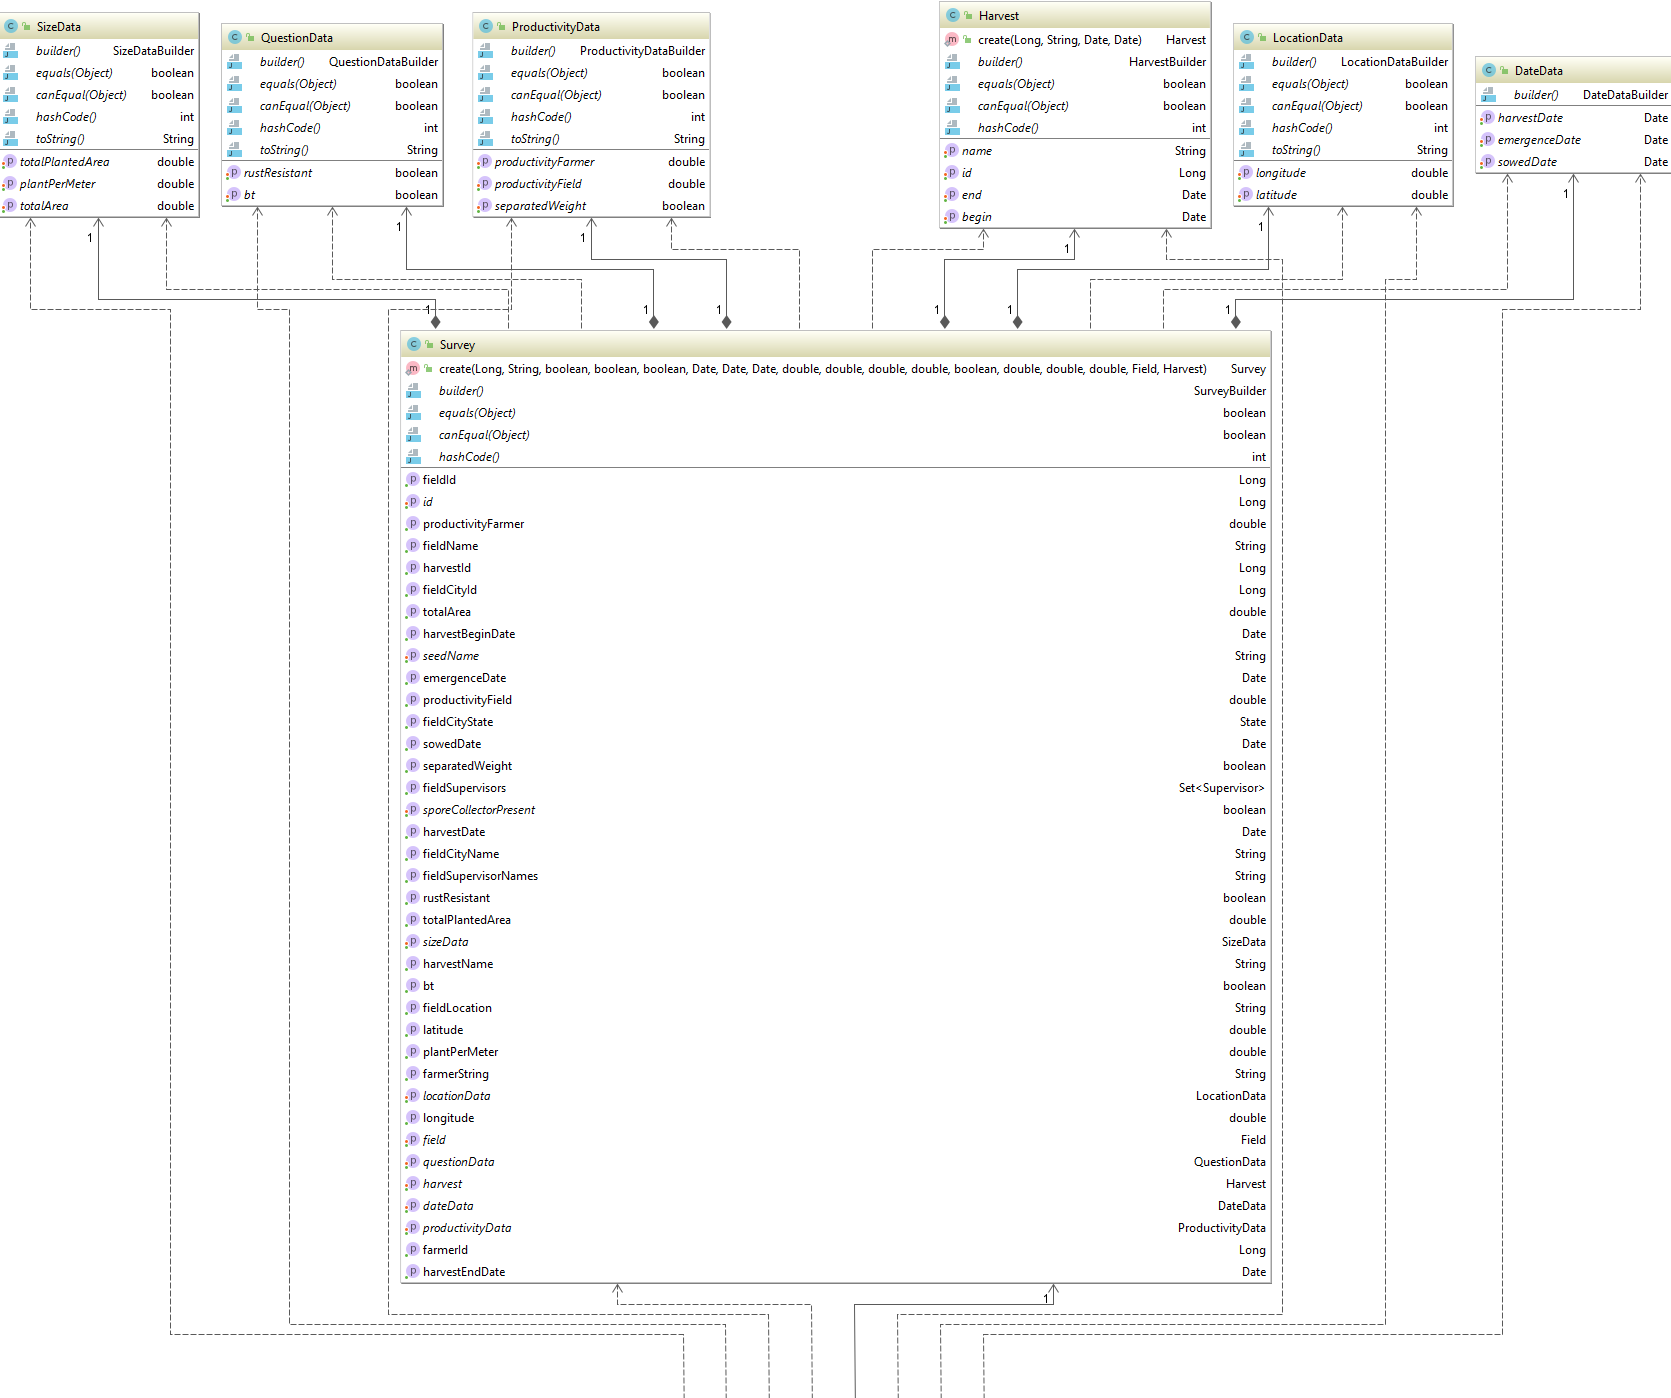
\includegraphics[scale=0.38]{dados/figuras/packSurvei.png}
\end{figure}

\begin{figure}[H]
	\centering
	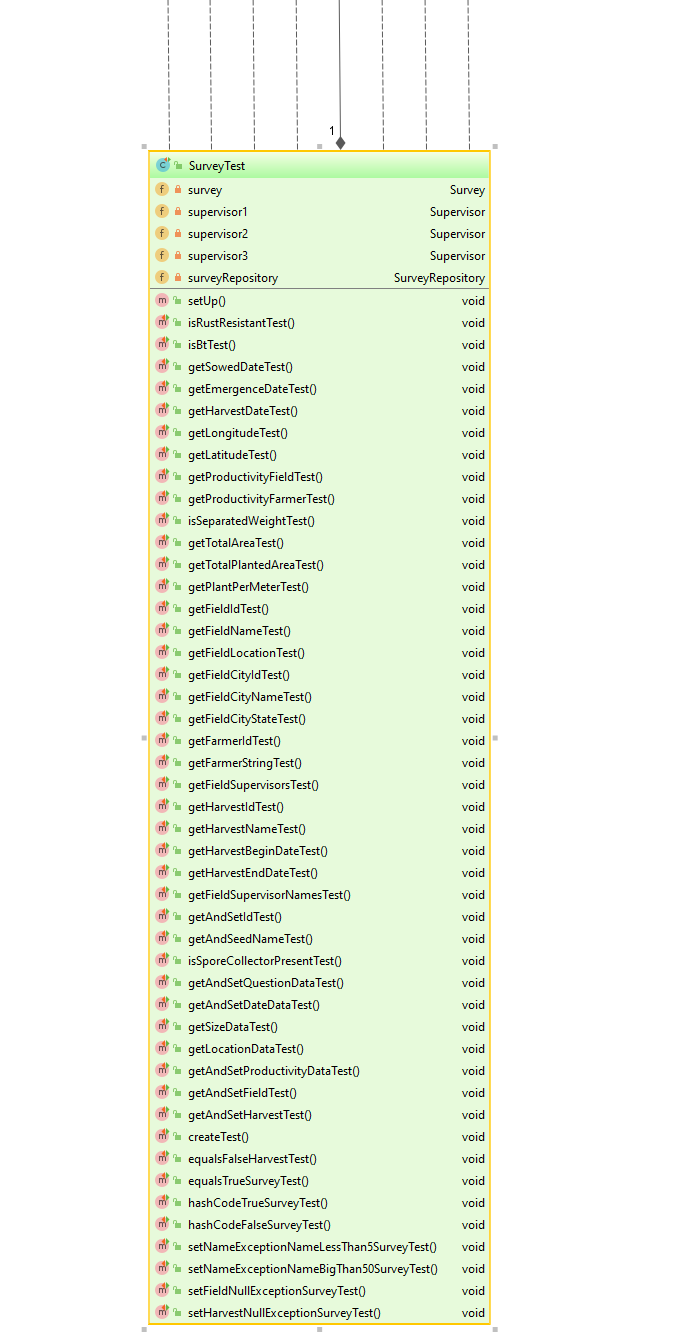
\includegraphics[scale=0.7]{dados/figuras/surveyTest.png}
	\caption{Diagrama de classes Survey e SurveyTest.java.}
	\label{classesSurvey}
\end{figure}

A classe de teste apresentada na FIGURA \ref{classesSurvey} possui 46 métodos de teste é um método de apoio aos testes denominado \textit{“setUp”}, o objetivo dos testes é exercitar a classe \textit{Survey} até que todos as variáveis, entradas e saídas de dados sejam executados pelo menos uma vez. Como a classe \textit{Survey} é composta por outras classes se faz necessário a instanciação de outras classes como \textit{Harvest}, \textit{Farmer}, \textit{City}, \textit{SizeData} e outras para a execução completa dos testes. Como a classe se trata de uma entidade que será persistida em um banco de dados, ela possui certas regras de negócio que serão ativadas somente no momento de gravar os dados no banco, sendo assim foi preciso criar uma referência para a interface \textit{SurveyRepository}, classe responsável por realizar a persistência dos dados no banco. Como o objetivo deste trabalho é cobrir o sistema com testes unitários e testes que integram classes entidades com o banco de dados ou comunicação com \textit{APIs} são testes de integração foi utilizado um \textit{“Mock”} para simular o comportamento do repositório.


A FIGURA \ref{testSurvey} apresenta a declaração da classe de teste, os atributos utilizados para desenvolver os testes e o método \textit{“setUp”} utilizado para preparar o ambiente para os testes.

O trecho de código da FIGURA \ref{testSurvey} apresenta as seguintes funcionalidades:

\begin{itemize}

    \item Na linha 1 é utilizada a anotação \textit{@FixMethodOrder} que permite definir uma ordem de execução dos testes, neste casso foi definida a ordem \textit{“NAME\_ASCENDING"} que faz a execução dos testes de acordo com o nome de maneira ascendente;
    
    \item Linha 2 a classe \textit{SurveyTest} é aberta;

    \item Na linha 4 é feita a declaração do objeto \textit{Survey}, nas linhas 5, 6 e 7  são declarados e instanciados objetos do tipo \textit{Supervisor};

    \item Na linha 8 um objeto do tipo \textit{SurveyRepositorio} é declarado e instanciado como um objeto \textit{mock};

    \item Na linha 10 é utilizado a anotação \textit{@Before}, esta anotação determina que sempre antes da execução de um teste o método \textit{“setUp”} deve ser executado primeiro.

    \item O método \textit{“setUp”} que tem sua declaração na linha 11 e vai até a linha 32, ele é responsável por realizar a construção do objeto \textit{Survey} declarado na linha 4.

\end{itemize}{}


A FIGURA \ref{testSurvey} apresenta os casos de testes criados para a classe \textit{Survey}. 


A ideia geral na elaboração dos testes é a de cobrir cada atribuição de dados, as entrada e saída de dados da classe \textit{Survey}, buscando a cobertura de 100\% das linhas métodos e atributo da classe. Os resultados obtidos da execução dos testes foram listados a seguir:



\begin{figure}[H]
	\centering
	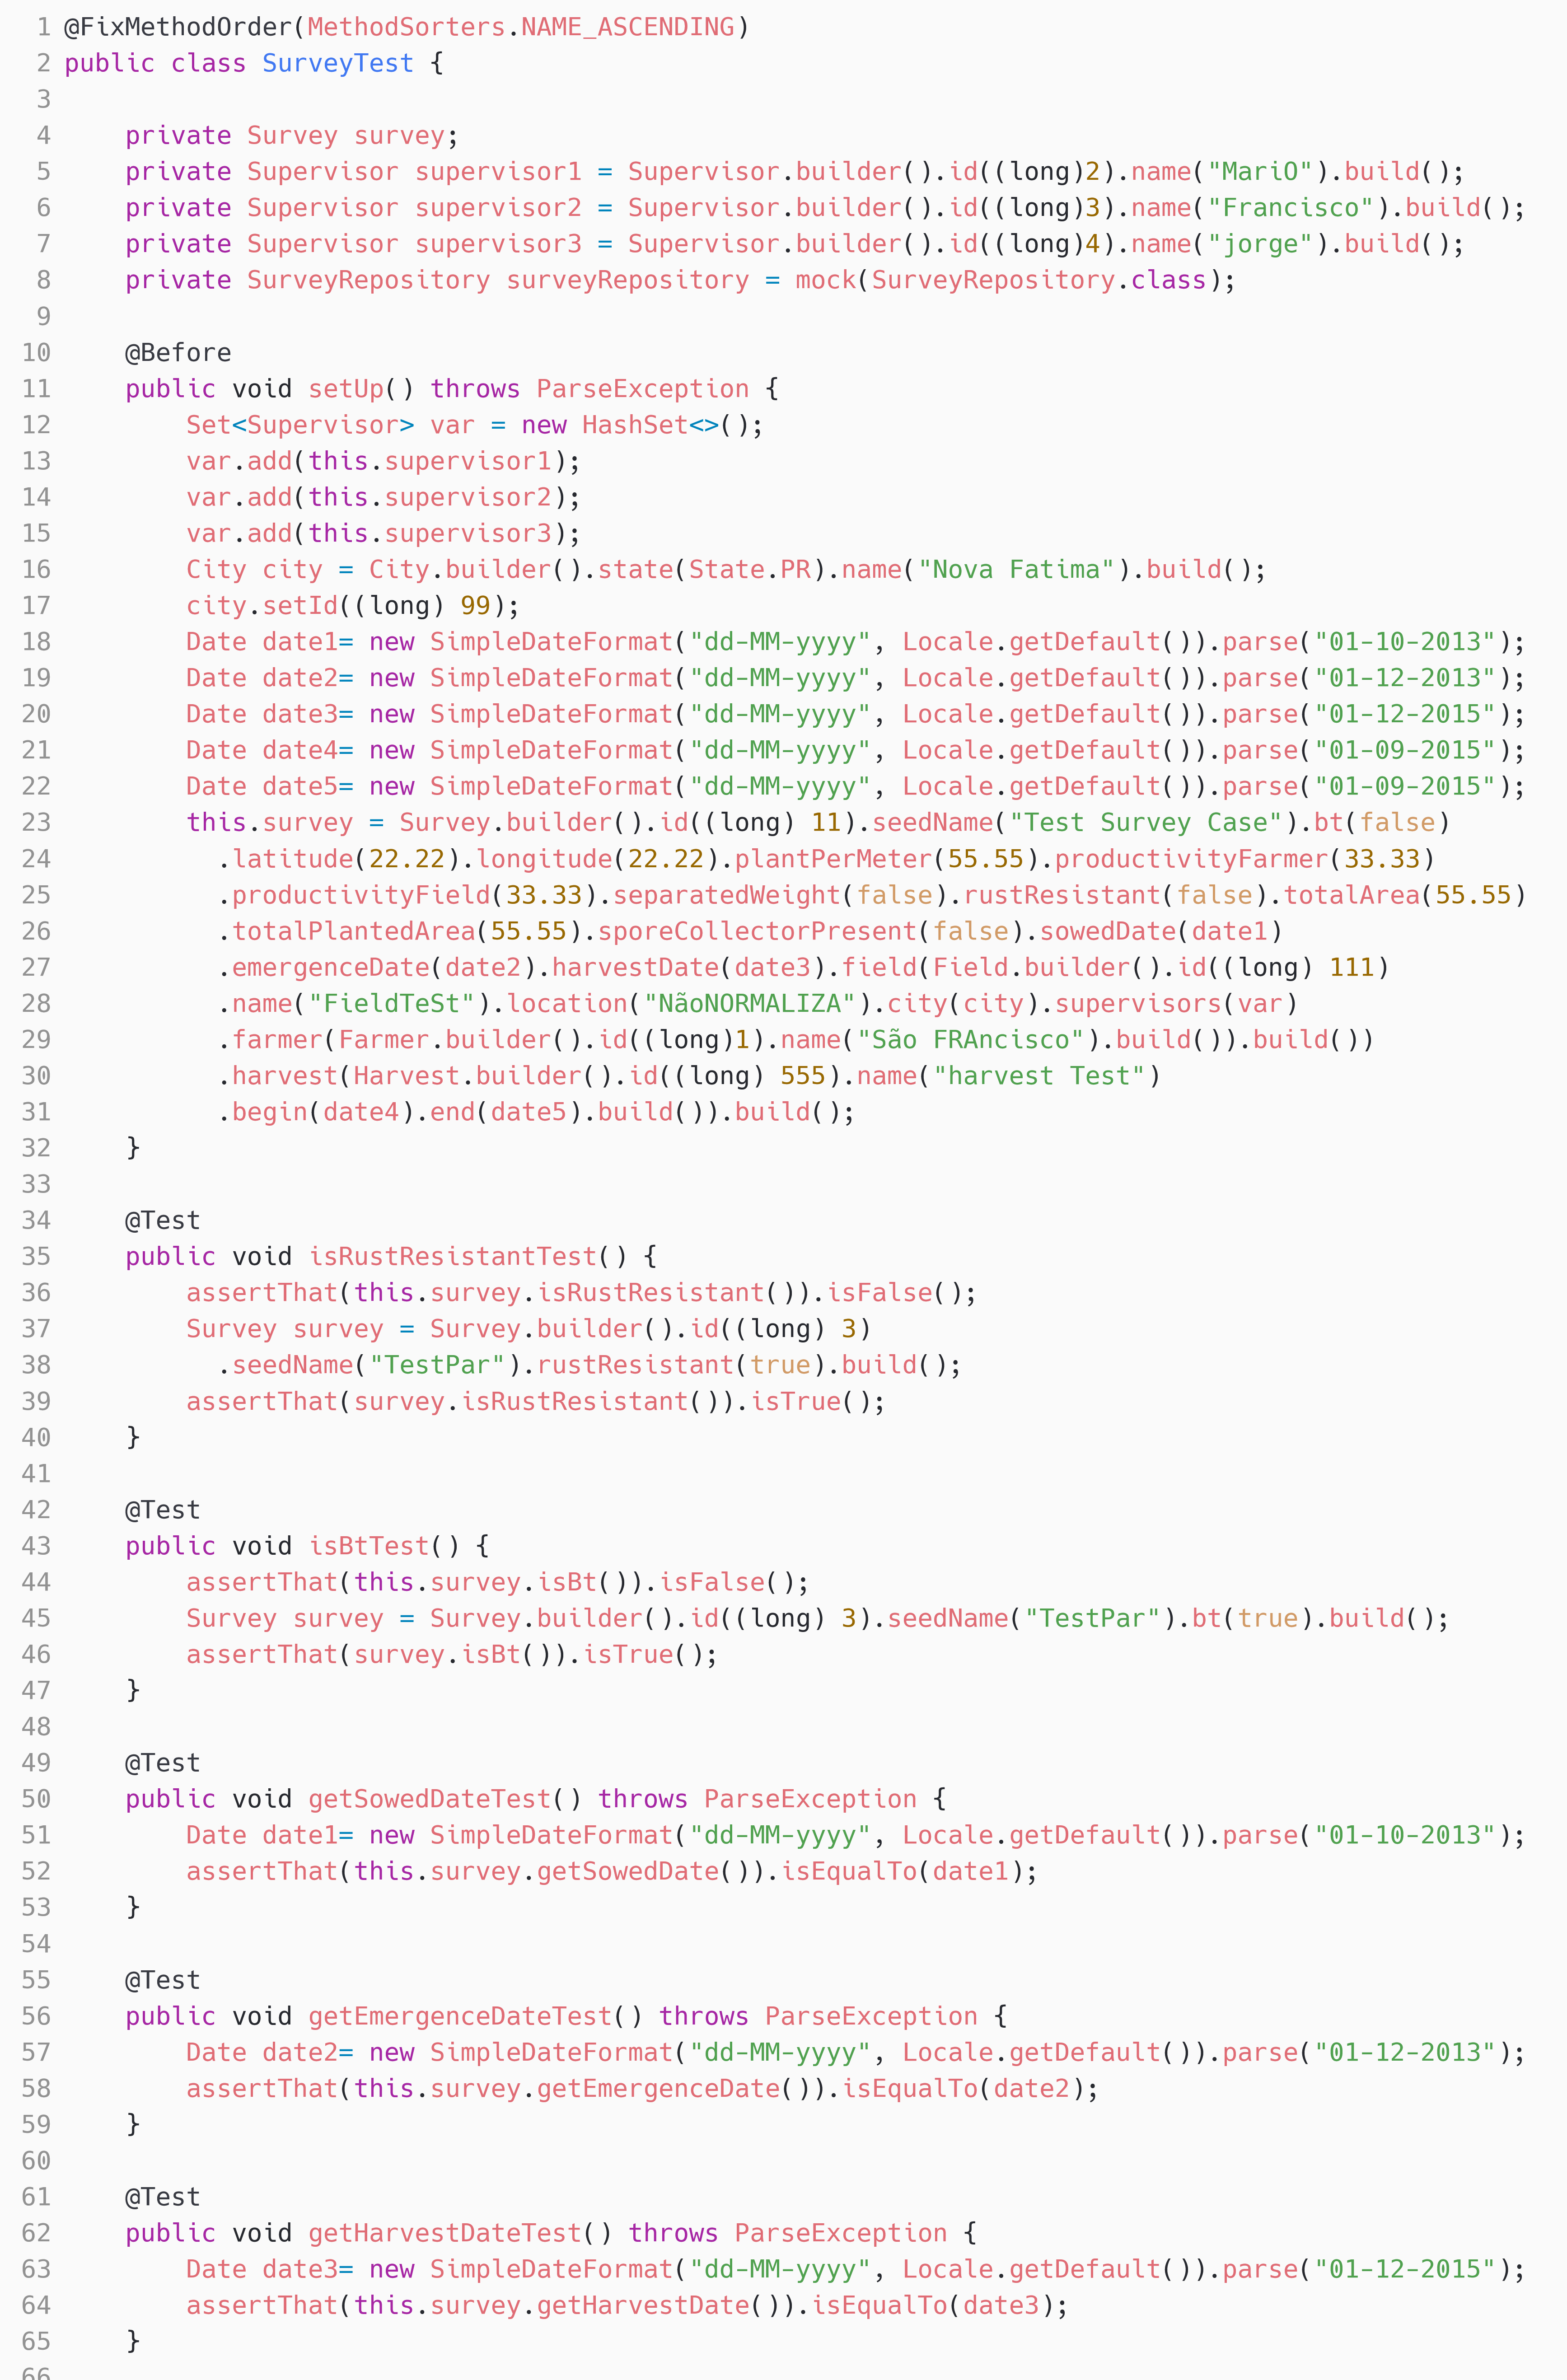
\includegraphics[scale=0.17]{dados/figuras/buildSurvey.png}
\end{figure}

\begin{figure}[H]
	\centering
	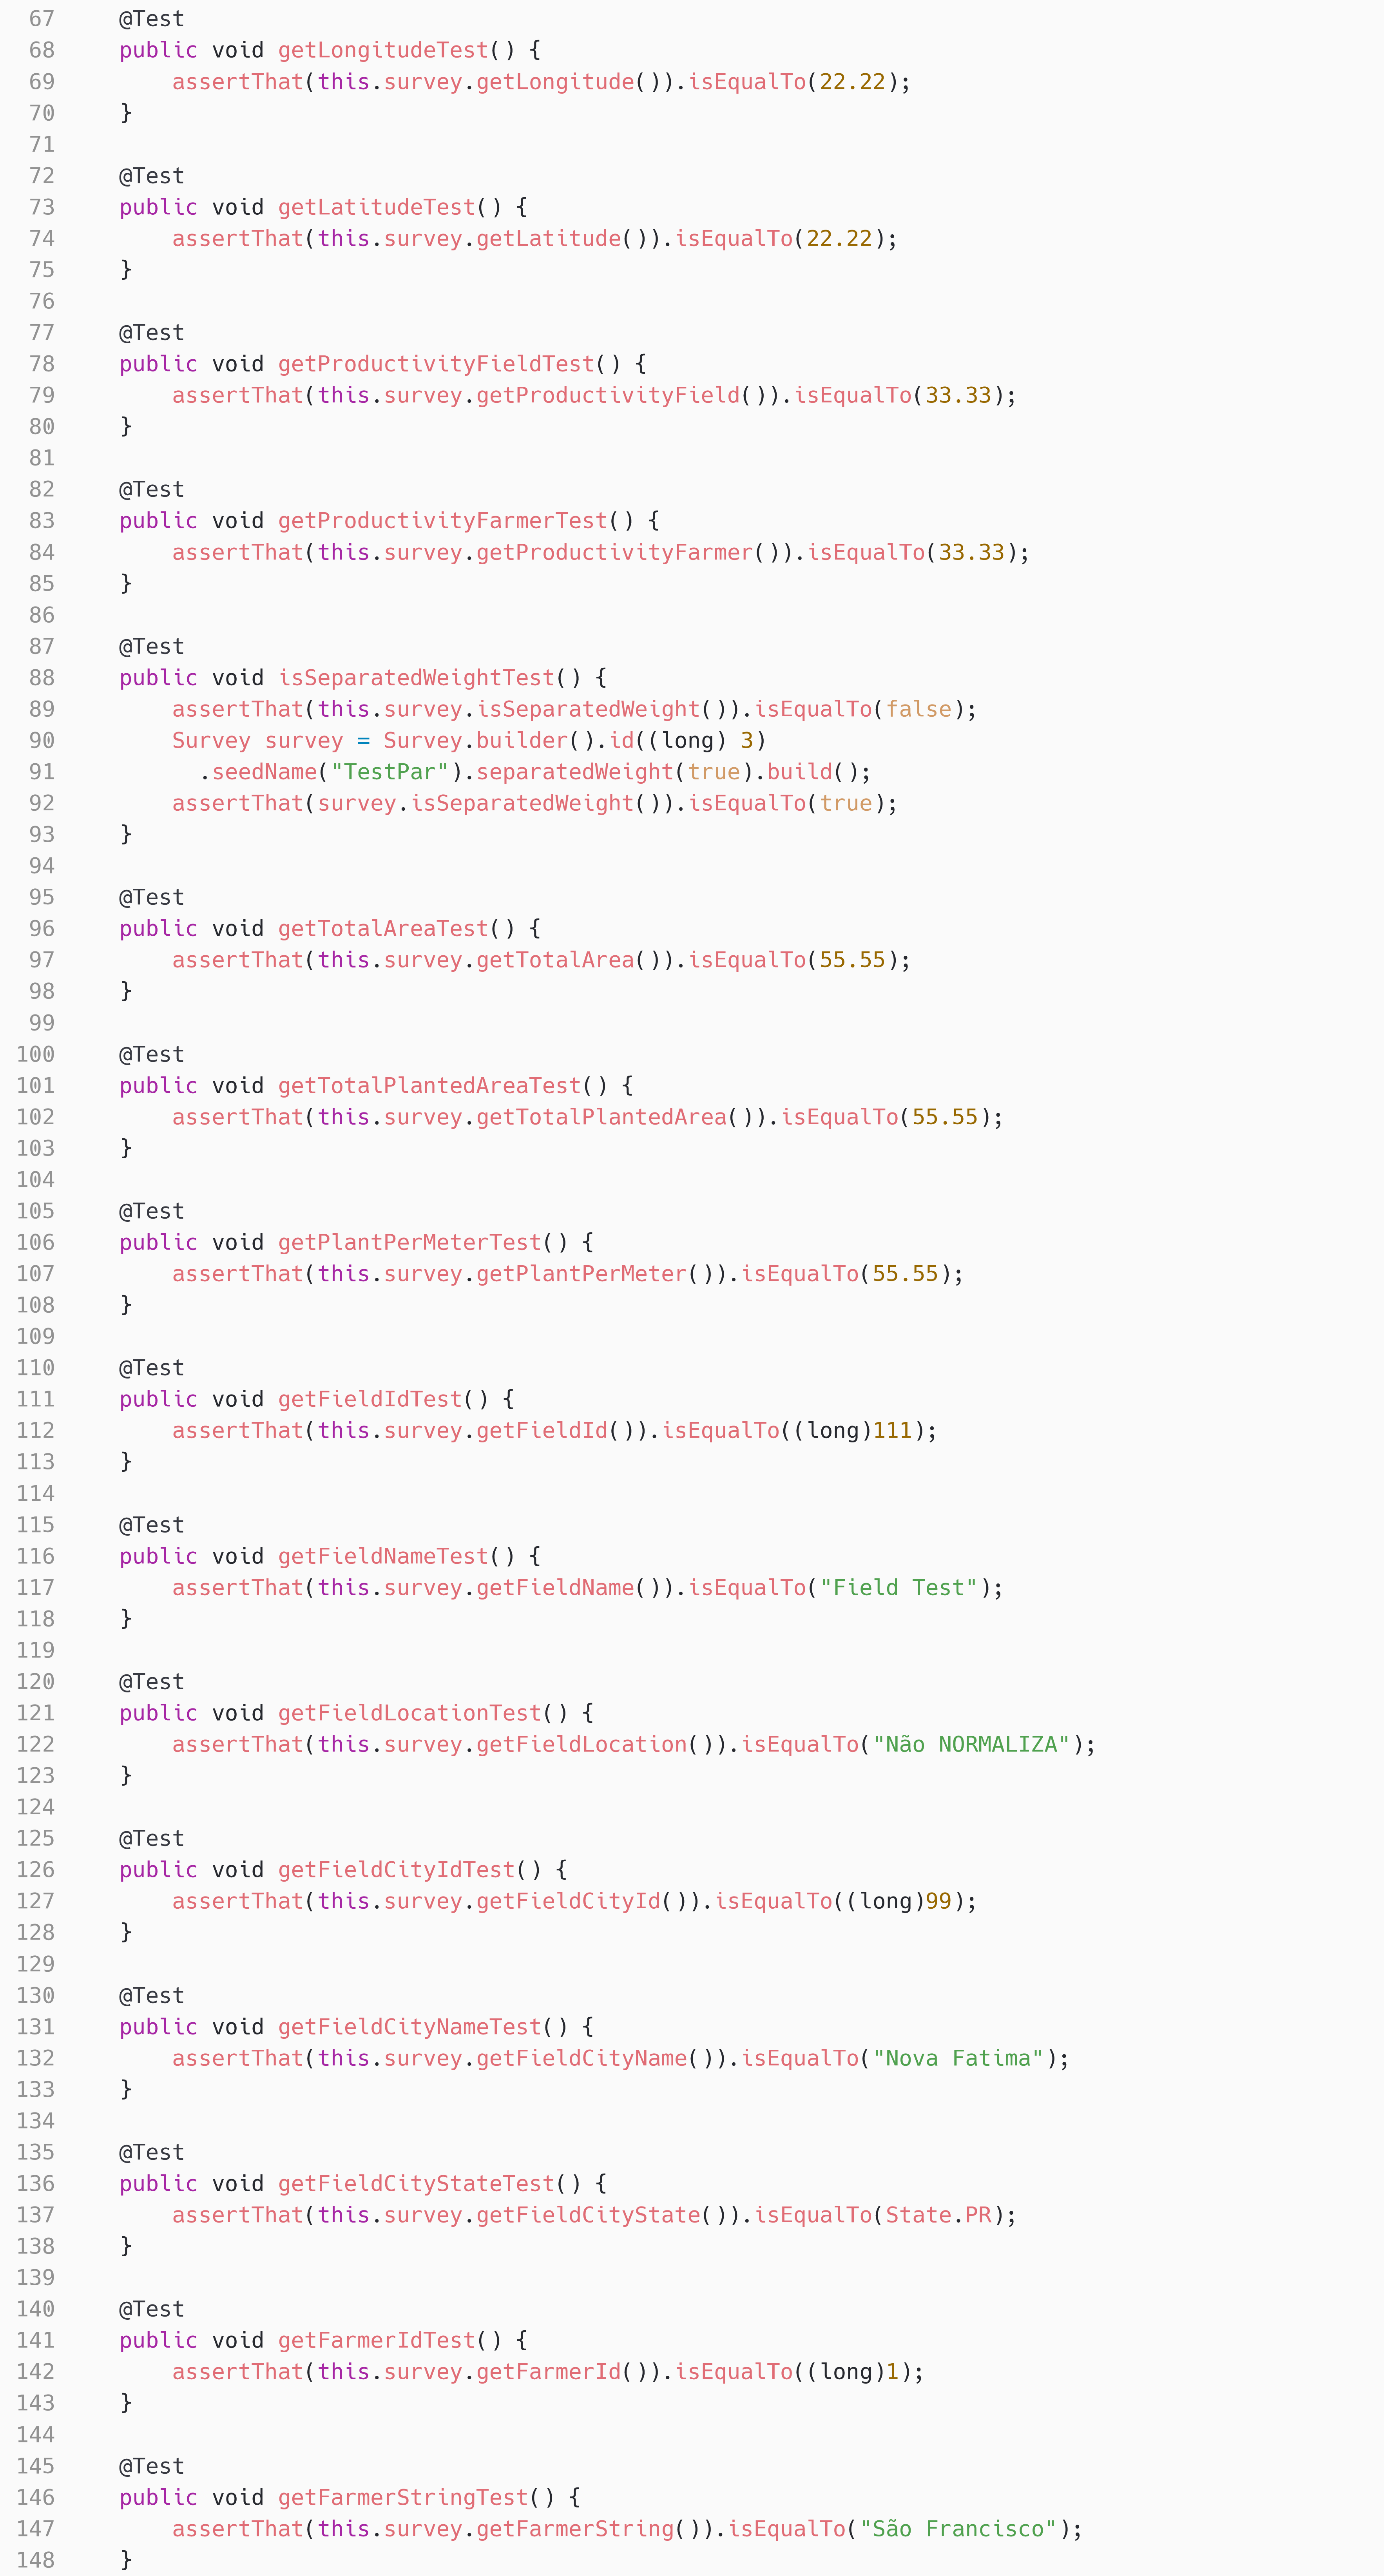
\includegraphics[scale=0.14]{dados/figuras/surveyTest1.png}
\end{figure}

\begin{figure}[H]
	\centering
	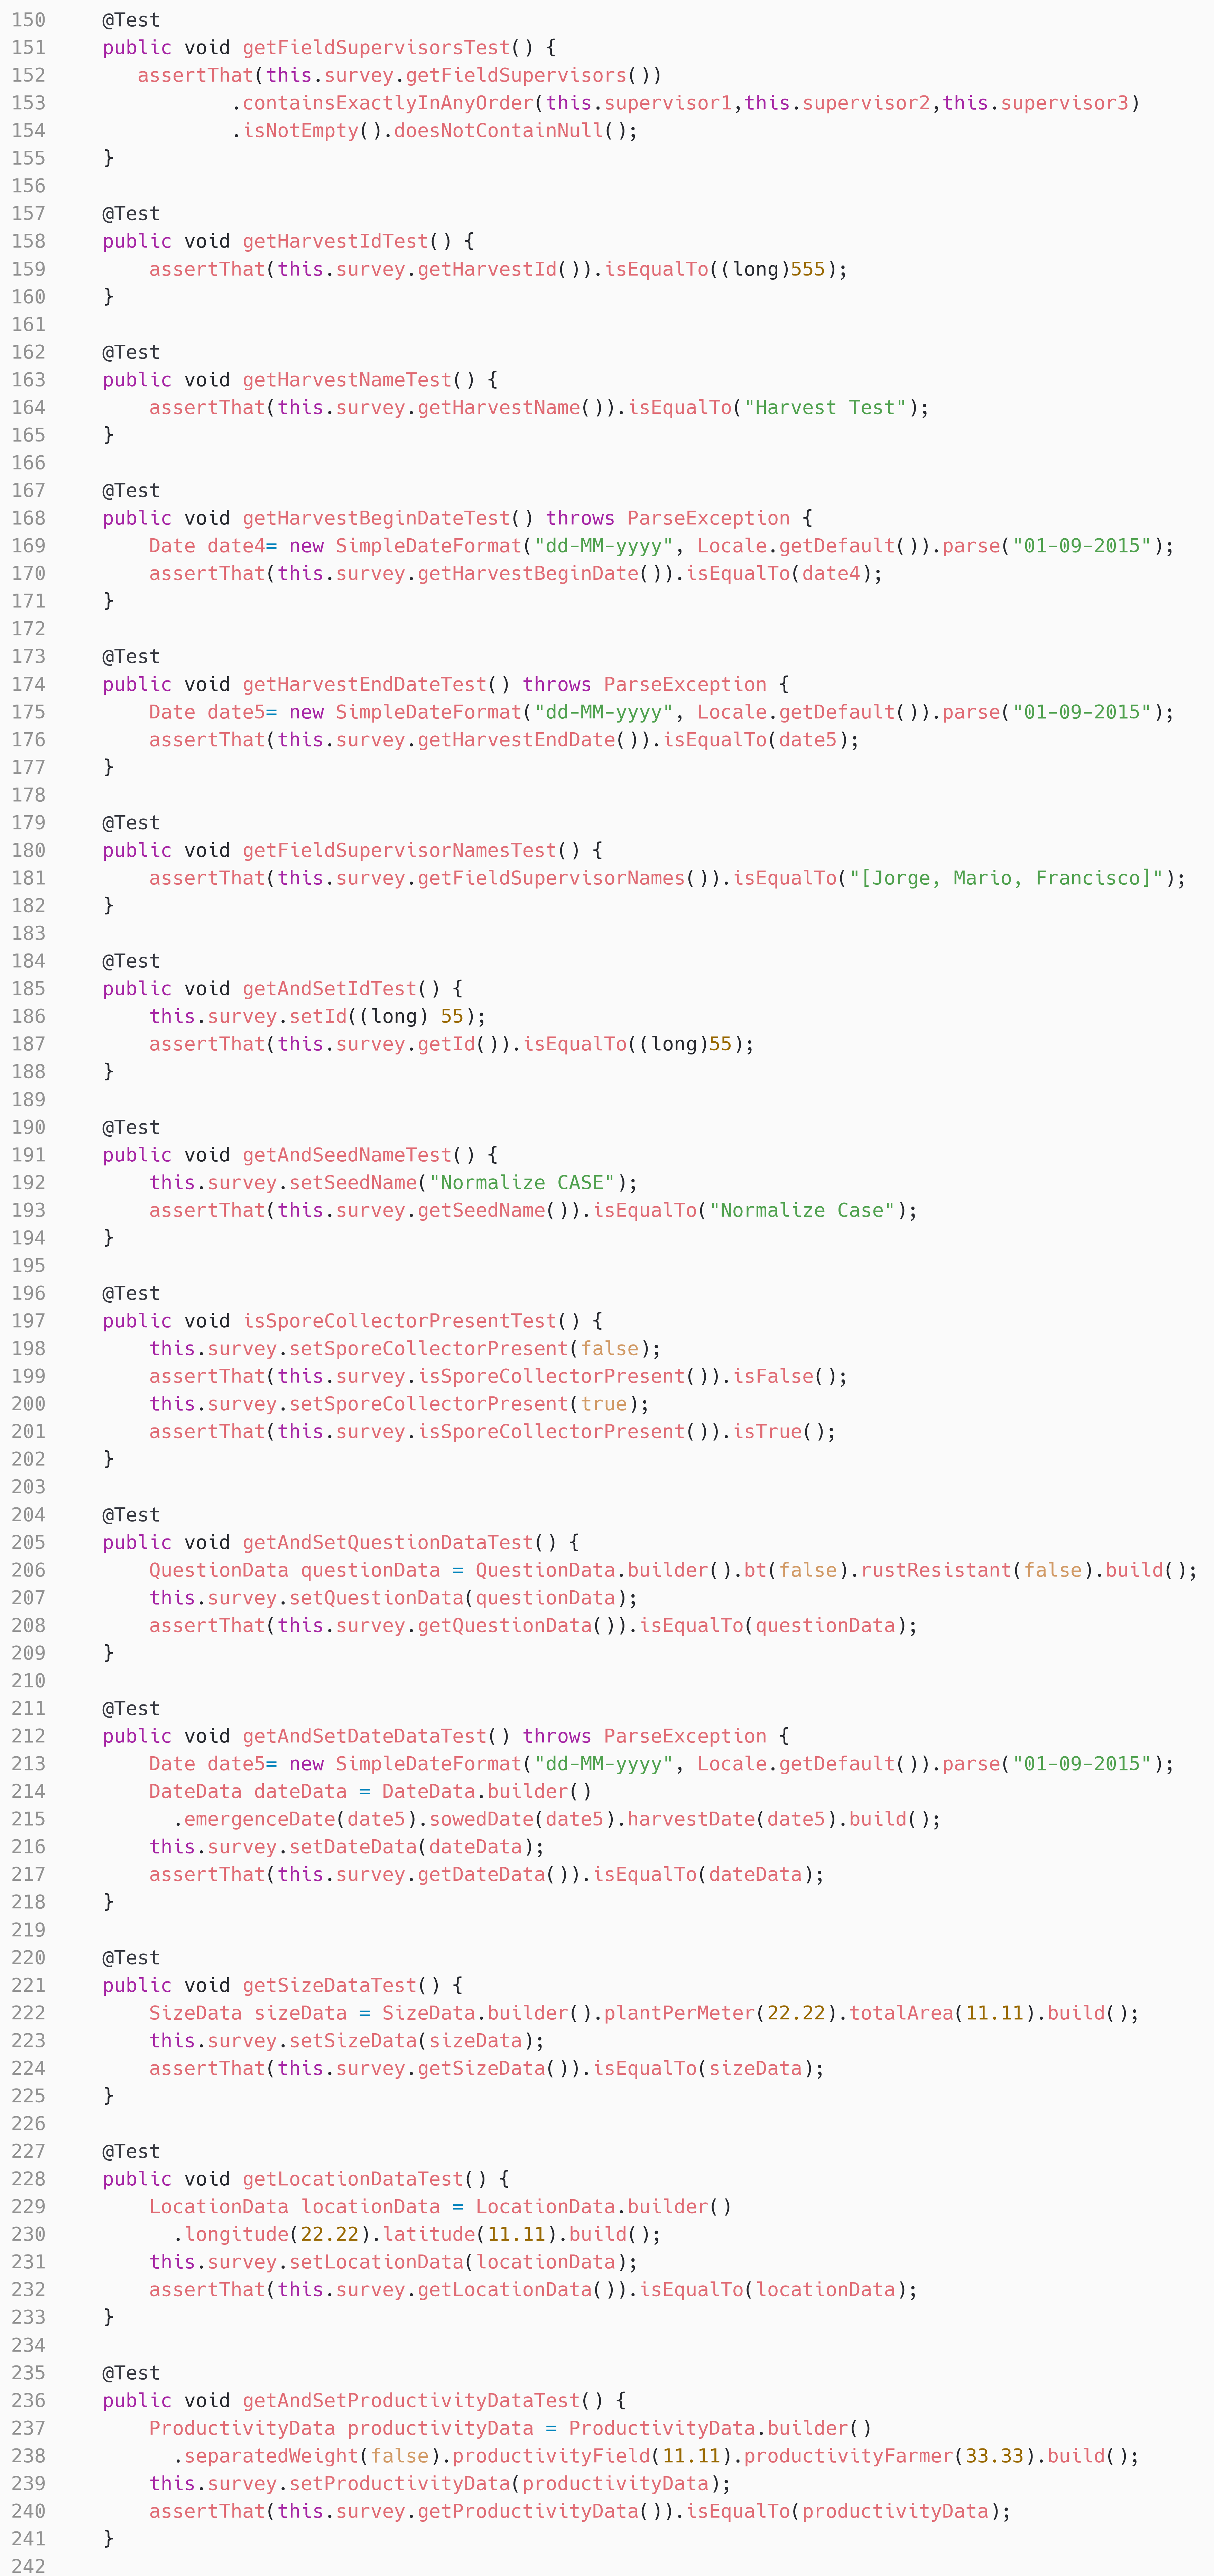
\includegraphics[scale=0.13]{dados/figuras/surveyTest2.png}
\end{figure}

\begin{figure}[H]
	\centering
	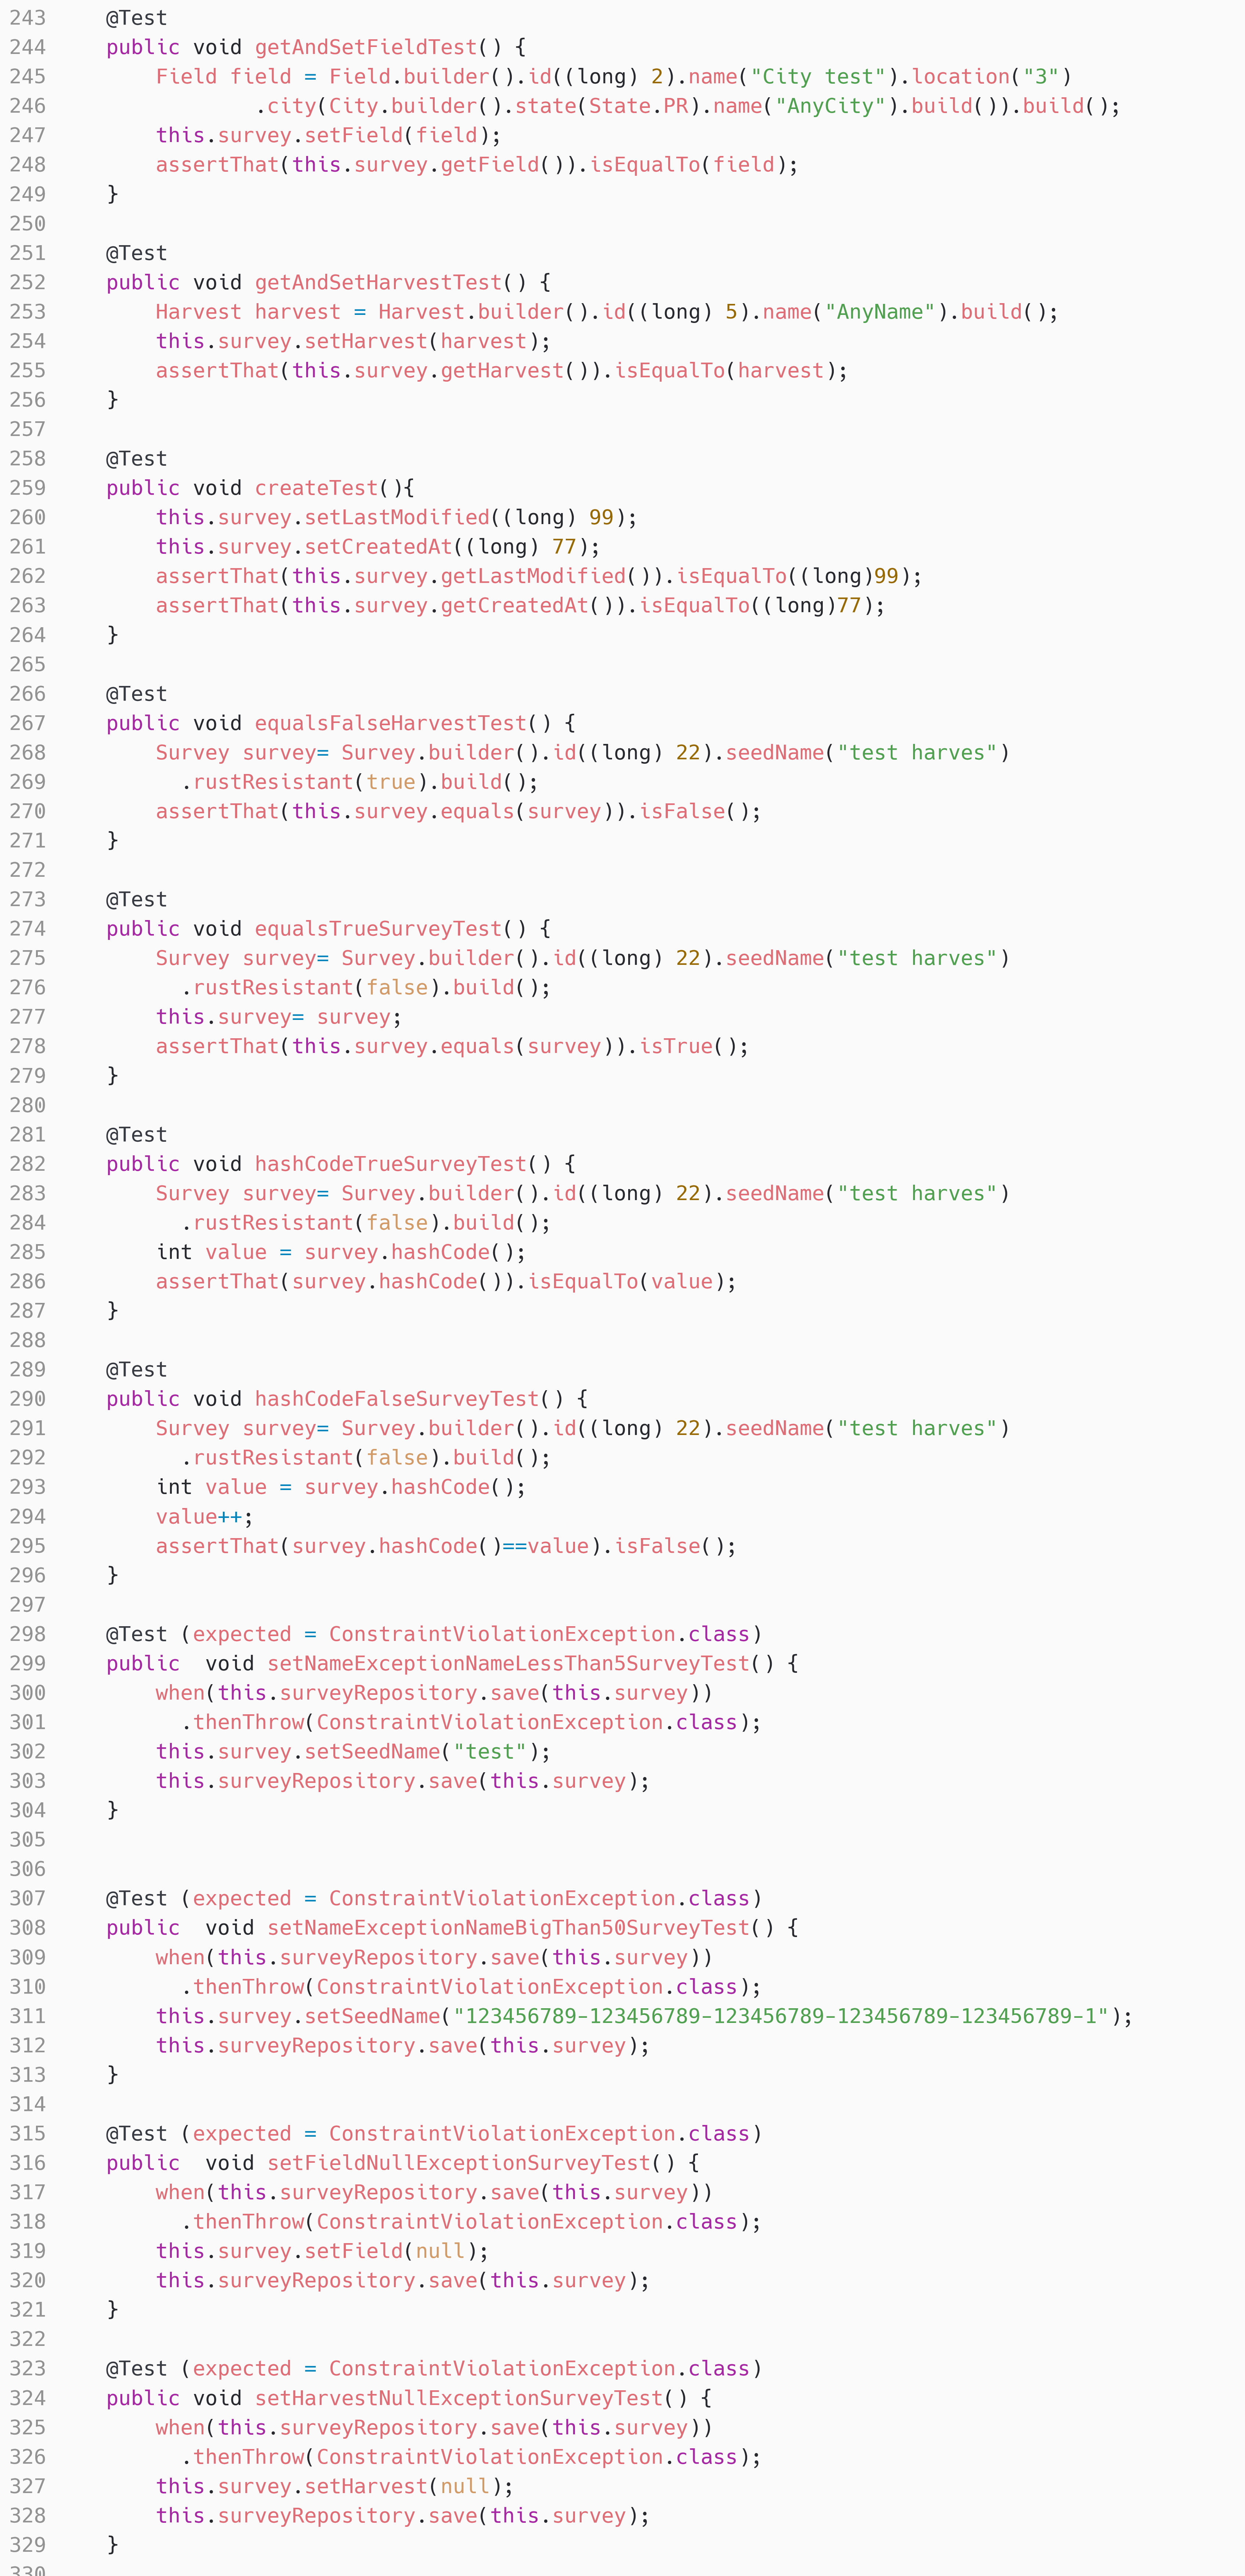
\includegraphics[scale=0.13]{dados/figuras/surveyTest3.png}
	\caption{Classe de Teste SurveyTest.java.}
	\label{testSurvey}
\end{figure}

Método de teste\textit{ “isRustResistantTest()”} linhas 34 a 40 figura \ref{testSurvey}:  Este método de teste consiste em recuperar o valor atribuído a variável\textit{ “rustResistant”} do objeto \textit{“Survey”.} A entrada é um \textit{“boolean”}(verdadeiro ou falso), a saída também se trata de um \textit{“boolean”}. A primeira assertiva recupera o valor atribuído na linha 25, \textit{“FALSE”}, e a saída do meto testado é um\textit{ “FALSE”}, linha 36, em seguida é atribuído a variável o valor \textit{“TRUE”}, linha 37 e 38, uma nova assertiva é feita e o valor recuperado é um \textit{“TRUE”}, linha 39.

Método de teste \textit{“isBtTest ()”} linhas 42 a 47 figura \ref{testSurvey}: Este método de teste consiste em recuperar o valor atribuído a variável\textit{ “bt”} do objeto \textit{“Survey”}. A entrada e um \textit{“boolean”}(verdadeiro ou falso), a saída também se trata de um \textit{“boolean”}. A primeira assertiva recupera o valor atribuído na linha 23, \textit{“FALSE”}, e a saída do meto testado é um \textit{“FALSE”}, linha 44, em seguida é atribuída a variável o valor \textit{“TRUE”}, linha 45 e 46, uma nova assertiva é feita e o valor recuperado é um \textit{“TRUE”}, linha 46.

Método de teste \textit{“getSowedDateTest()”} linhas 49 a 53 figura \ref{testSurvey}: Este teste consiste em recuperar a data atribuída a variável “\textit{“SowedDate”}” do objeto \textit{“Survey”}. A entrada é um objeto do tipo “\textit{“Date”}” que contém o valor de uma data com dia, mês e ano. A saída é um objeto do tipo “\textit{“Date”}” que contem o valor de uma data válida. A entrada é definida na linha 26, um outro objeto do tipo \textit{“Date”} é criado para comparação na linha 51. A assertiva é feita na linha 52 e compara o valor recuperado do meto testado com o valor definido na linha 51, os valores são iguais.  

Método de teste \textit{“getEmergenceDateTest()”} linhas 55 a 59 figura \ref{testSurvey}: Este teste consiste em recuperar a data atribuída a variável \textit{“EmergenceDate”} do objeto \textit{“Survey”}. A entrada é um objeto do tipo \textit{“Date”} que contém o valor de uma data com dia, mês e ano. A saída é um objeto do tipo \textit{“Date”} que contém o valor de uma data válida. A entrada é definida na linha 27, um outro objeto do tipo \textit{“Date”} é criado para comparação na linha 57. A assertiva é feita na linha 58 e compara o valor recuperado do meto testado com o valor definido na linha 57, os valores são iguais.  

Método de teste \textit{“getHarvestDateTest()”} linhas 61 a 65 figura \ref{testSurvey}: Este teste consiste em recuperar a data atribuída a variável \textit{“HarvestDate”} do objeto \textit{“Survey”}. A entrada é um objeto do tipo \textit{“Date”} que contém o valor de uma data com dia, mês e ano. A saída é um objeto do tipo \textit{“Date”} que contém o valor de uma data válida. A entrada é definida na linha 27, um outro objeto do tipo \textit{“Date”} é criado para comparação na linha 63. A assertiva é feita na linha 64 e compara o valor recuperado do meto testado com o valor definido na linha 63, os valores são iguais.  

Método de teste \textit{“getLongitudeTest()”} linhas 67 a 71 figura \ref{testSurvey}: Este teste consiste em recuperar o valor atribuído a variável \textit{“Longitude” }do objeto \textit{“LocationData”}  presente em uma pesquisa. A entrada consiste em um valor numérico de ponto flutuante \textit{“Double”} e a saída também consiste em um valor numérico do tipo \textit{“Double”}. A entrada é realizada na linha 24, o método é testado na linha 69, o retorno é o mesmo valor atribuído na linha 24.   

Método de teste \textit{“getLatitudeTest()”} linhas 72 a 75 figura \ref{testSurvey}: Este teste consiste em recuperar o valor atribuído a variável\textit{ “Latitude”} do objeto \textit{“LocationData”} presente em uma pesquisa. A entrada consiste em um valor numérico de ponto flutuante \textit{“Double”} e a saída também consiste em um valor numérico do tipo \textit{“Double”}. A entrada é realizada na linha 24, o método é testado na linha 74, o retorno é o mesmo valor atribuído na linha 24.

Método de teste \textit{“getProductivityFieldTest()”} linhas 77 a 80 figura \ref{testSurvey}: Este teste consiste em recuperar o valor atribuído a variável “productivityField” do objeto \textit{“ProductivityData”} presente em uma pesquisa. A entrada consiste em um valor numérico de ponto flutuante \textit{“Double”} e a saída também consiste em um valor numérico do tipo \textit{“Double”}. A entrada é realizada na linha 24, o método é testado na linha 74, o retorno é o mesmo valor atribuído na linha 24.

Método de teste \textit{“getProductivityFarmerTest()”} linhas 82 a 85 figura \ref{testSurvey}: Este teste consiste em recuperar o valor atribuído a variável\textit{ “productivityFarmer”} do objeto \textit{“ProductivityData”} presente em uma pesquisa. A entrada consiste em um valor numérico de ponto flutuante \textit{“Double”} e a saída também consiste em um valor numérico do tipo \textit{“Double”}. A entrada é realizada na linha 24, o método é testado na linha 79, o retorno é o mesmo valor atribuído na linha 24.

Método de teste \textit{“isSeparatedWeightTest()”} linhas 87 a 93 figura \ref{testSurvey}: Este método de teste consiste em recuperar o valor atribuído a variável\textit{ “SeparatedWeight”} do objeto \textit{“ProductivityData”} presente em uma pesquisa. A entrada e um \textit{“boolean”}(verdadeiro ou falso), a saída também se trata de um \textit{“boolean”}. A primeira assertiva recupera o valor atribuído na linha 25, \textit{“FALSE”}, e a saída do meto testado é um \textit{“FALSE”}, linha 44, em seguida é atribuída a variável o valor \textit{“TRUE”}, linha 90 e 91, uma nova assertiva é feita é o valor recuperado é um \textit{“TRUE”}, linha 92.

Método de teste \textit{“getTotalAreaTest()”} linhas 95 a 98 figura \ref{testSurvey}: Este teste consiste em recuperar o valor atribuído a variável\textit{ “TotalArea”} do objeto \textit{“SizeData”} presente em uma pesquisa. A entrada consiste em um valor numérico de ponto flutuante \textit{“Double”} e a saída também consiste em um valor numérico do tipo \textit{“Double”}. A entrada é realizada na linha 25, o método é testado na linha 97, o retorno é o mesmo valor atribuído na linha 25.

Método de teste \textit{“getTotalPlantedAreaTest()”} linhas 100 a 103 figura \ref{testSurvey}: Este teste consiste em recuperar o valor atribuído a variável \textit{“TotalPlantedArea”} do objeto \textit{“SizeData”} presente em uma pesquisa. A entrada consiste em um valor numérico de ponto flutuante \textit{“Double”} e a saída também consiste em um valor numérico do tipo \textit{“Double”}. A entrada é realizada na linha 26, o método é testado na linha 102, o retorno é o mesmo valor atribuído na linha 26.

Método de teste \textit{“getPlantPerMeterTest()”} linhas 105 a 108 figura \ref{testSurvey}: Este teste consiste em recuperar o valor atribuído a variável\textit{ “plantPerMeter”} do objeto \textit{“SizeData”} presente em uma pesquisa. A entrada consiste em um valor numérico de ponto flutuante \textit{“Double”} e a saída também consiste em um valor numérico do tipo \textit{“Double”}. A entrada é realizada na linha 24, o método é testado na linha 107, o retorno é o mesmo valor atribuído na linha 24.

Método de teste \textit{“getFieldIdTest()”} linhas 110 a 113 figura \ref{testSurvey}: Este teste consiste em recuperar o identificador único de um objeto \textit{“Field”} presente em uma pesquisa. A entrada consiste em um objeto do tipo \textit{“Field”} que possui um identificador único, a saída é o identificador único, um valor numérico do tipo \textit{“Long”}. A entrada é feita nas linhas 27 e 28, a assertiva é feia na linha 112, o valor recuperado é o mesmo atribuído na linha 27.

Método de teste\textit{ “getFieldNameTest()”} linhas 115 a 118 figura \ref{testSurvey}: Este teste consiste em recuperar o nome atribuído a um objeto \textit{“Field”} presente em uma pesquisa. A entrada consiste em um objeto do tipo \textit{“Field”} que possui um nome, a saída é o nome contido no objeto, uma \textit{String”} de caracteres normalizados com o primeiro caractere de cada conjunto de caracteres maiúsculo. A entrada é feita nas linhas 27 e 28, a assertiva é feia na linha 117, o valor recuperado é o mesmo atribuído na linha 27 mais com o primeiro caractere de cada conjunto maiúsculo.

Método de teste \textit{“getFieldLocationTest()”} linhas 120 a 123 figura \ref{testSurvey}: Este teste consiste em recuperar a localização atribuída a um objeto \textit{“Field”} presente em uma pesquisa. A entrada consiste em um objeto do tipo \textit{“Field”} que possui uma localização, a saída é a localização contida no objeto, uma \textit{“String”} de caracteres. A entrada é feita nas linhas 27 e 28, a assertiva é feia na linha 122, o valor recuperado é o mesmo atribuído na linha 27.

Método de teste\textit{ “getFieldCityIdTest()”} linhas 125 a 128 figura \ref{testSurvey}: Este teste consiste em recuperar o identificador único de um objeto \textit{“City”} presente em uma pesquisa. A entrada consiste em um objeto do tipo \textit{“Field”} que possui uma cidade com identificador único, a saída é o identificador do único da cidade, um valor numérico do tipo \textit{“Long”}. O objeto \textit{“City”} é criado nas linhas 16 e 17, a entrada é feita nas linhas 27 e 28, a assertiva é feia na linha 127, o valor recuperado é o mesmo atribuído na linha 17.


Método de teste \textit{“getFieldCityNameTest()”} linhas 130 a 133 figura \ref{testSurvey}: Este teste consiste em recuperar o nome de um objeto \textit{“City”} presente em uma pesquisa. A entrada consiste em um objeto do tipo \textit{“Field”} que possui uma cidade com um nome, a saída é uma \textit{“String”} de caracteres normalizados com o primeiro caractere de cada conjunto maiúsculo. O objeto \textit{“City”} é criado nas linhas 16, a entrada é feita nas linhas 27 e 28, a assertiva é feia na linha 132, o valor recuperado é o mesmo atribuído na linha 16 mais com o primeiro caractere de cada conjunto maiúsculo.

Método de teste \textit{“getFieldCityStateTest()”} linhas 135 a 138 figura \ref{testSurvey}: Este teste consiste em recuperar o estado de um objeto \textit{“City”} presente em uma pesquisa. A entrada consiste em um objeto do tipo \textit{“Field”} que possui uma cidade com um estado, a saída é um objeto do tipo \textit{“State.PR”}. O objeto \textit{“City”} é criado nas linhas 16, a entrada é feita nas linhas 27 e 28, a assertiva é feia na linha 137, o valor recuperado é o mesmo atribuído na linha 16.

Método de teste \textit{“getFarmerIdTest()”} linhas 140 a 143 figura \ref{testSurvey}: Este teste consiste em recuperar o identificador único de um objeto \textit{“Farmer”} presente em uma pesquisa. A entrada consiste em um objeto do tipo \textit{“Field”} que possui um agricultor com identificador único, a saída é o identificador do único do agricultor, um valor numérico do tipo \textit{“Long”}. O objeto \textit{“Farmer”} é criado na linha 29, a entrada é feita na linha 27, 28 e 29, a assertiva é feia na linha 142, o valor recuperado é o mesmo atribuído na linha 29.

Método de teste \textit{“getFarmerStringTest()”} linhas 145 a 148 figura \ref{testSurvey}: Este teste consiste em recuperar o nome de um objeto \textit{“Farmer”} presente em uma pesquisa. A entrada consiste em um objeto do tipo \textit{“Field”} que possui um agricultor com um nome, a saída é uma \textit{“String”} de caracteres normalizados com o primeiro caractere de cada conjunto maiúsculo. O objeto \textit{“Farmer”} é criado nas linhas 29, a entrada é feita nas linhas 27, 28 e 29, a assertiva é feia na linha 147, o valor recuperado é o mesmo atribuído na linha 29 mais com o primeiro caractere de cada conjunto maiúsculo.

Método de teste \textit{“getFieldSupervisorsTest()”} linhas 150 a 155 figura \ref{testSurvey}: Este teste consiste em recuperar os supervisores presentes em um objeto \textit{“Field”} presente em uma pesquisa. A entrada consiste em um objeto do tipo \textit{“Field”} que possua um ou mais supervisores, a saída é uma lista de objetos do tipo \textit{“Supervisor”} que contem os supervisores presentes no \textit{“Field”} presente na pesquisa. Uma lista de supervisores é criada nas linhas 12 a 15, a entrada é feita nas linhas 27, 28 e 29, a assertiva é feia nas linhas 152 e 153, o valor recuperado e uma lista de supervisores que contem os supervisores declarados nas linhas 5, 6 e 7.


Método de teste \textit{“getHarvestIdTest()”} linhas 157 a 160 figura \ref{testSurvey}: Este teste consiste em recuperar o identificador único de um objeto \textit{“Harvest”} presente em uma pesquisa. A entrada consiste em um objeto do tipo \textit{“Harvest”} que possui um identificador único, a saída é o identificador do único da colheita, um valor numérico do tipo \textit{“Long”}. O objeto \textit{“Harvest”} é criado na linha 30, a entrada é feita nas linhas 27, 28, 29 e 30 a assertiva é feia na linha 159, o valor recuperado é o mesmo atribuído na linha 30.

Método de teste \textit{“getHarvestNameTest()”} linhas 162 a 165 figura \ref{testSurvey}: Este teste consiste em recuperar o nome de um objeto \textit{“Harvest”} presente em uma pesquisa. A entrada consiste em um objeto do tipo \textit{“Harvest”} que possui um nome, a saída é uma \textit{“String”} de caracteres normalizados com o primeiro caractere de cada conjunto maiúsculo. O objeto \textit{“Harvest”} é criado nas linhas 30, a entrada é feita nas linhas 27, 28, 29 e 30, a assertiva é feia na linha 164, o valor recuperado é o mesmo atribuído na linha 30 mais com o primeiro caractere de cada conjunto maiúsculo.

Método de teste \textit{“getHarvestBeginDateTest()”} linhas 167 a 171 figura \ref{testSurvey}: Este teste consiste em recuperar a data da variável \textit{“BeginDate”} atribuída a um objeto \textit{“Harvest”} presente em uma pesquisa. A entrada é um objeto do tipo \textit{“Harvest”} que possui um \textit{“Date”} que contém o valor de uma data com dia, mês e ano. A saída é um objeto do tipo \textit{“Date”} que contém o valor de uma data válida. A entrada é definida na linha 30, um outro objeto do tipo \textit{“Date”} é criado para comparação na linha 169. A assertiva é feita na linha 170 e compara o valor recuperado do meto testado com o valor definido na linha 169, os valores são iguais.  

Método de teste \textit{“getHarvestEndDateTest()”} linhas 173 a 177 figura \ref{testSurvey}: Este teste consiste em recuperar a data da variável \textit{“EndDate” }atribuída a um objeto \textit{“Harvest”} presente em uma pesquisa. A entrada é um objeto do tipo \textit{“Harvest”} que possui um \textit{“Date”} que contém o valor de uma data com dia, mês e ano. A saída é um objeto do tipo \textit{“Date”} que contém o valor de uma data válida. A entrada é definida na linha 30, um outro objeto do tipo \textit{“Date”} é criado para comparação na linha 175. A assertiva é feita na linha 176 e compara o valor recuperado do meto testado com o valor definido na linha 175, os valores são iguais.  

Método de teste \textit{“getFieldSupervisorNamesTest()”} linhas 179 a 182 figura \ref{testSurvey}: Este teste consiste em recuperar os nomes dos supervisores presentes em um objeto \textit{“Field”} presente em uma pesquisa. A entrada consiste em um objeto do tipo \textit{“Field”} que possua um ou mais supervisores, a saída é uma \textit{“String”} que contém os nomes dos supervisores presentes no objeto \textit{“Field”} presente na pesquisa. Uma lista de supervisores é criada nas linhas 12 a 15, a entrada é feita nas linhas 27, 28 e 29, a assertiva é feia nas linhas 181, o valor recuperado e uma \textit{“String”} com o nome dos supervisores declarados nas linhas 5, 6 e 7.

Método de teste \textit{“getAndSetIdTest()”} linhas 184 a 188 figura \ref{testSurvey}: Este teste consiste em atribuir e recuperar o identificador único de uma pesquisa. A entrada consiste em um valor numérico do tipo \textit{“Long”}, a saída é um valor numérico do tipo \textit{“Long”}. A entrada e feita na linha 186, a saída e feita na assertiva linha 187, que compara a saída com o valor atribuído, os valores são iguais.

Método de teste \textit{“getAndSeedNameTest()”} linhas 190 a 194 figura \ref{testSurvey}: Este teste trata de atribuir um valor da variável \textit{“Seed”} do tipo \textit{“String”} do objeto \textit{“Survey”}. A entrada consiste em uma \textit{“String”} de caracteres, a saída é uma string de caracteres normalizada. A assertiva é feita na linha 193 e o valor recuperado é idêntico ao atribuído, mas com a primeira letra de cada conjunto de caracteres maiúscula.

Método de teste \textit{“isSporeCollectorPresentTest()”} linhas 196 a 202 figura \ref{testSurvey}: Este método de teste consiste em recuperar o valor atribuído a variável \textit{“SporeCollectorPresent” }do objeto \textit{“Survey”}. A entrada e um \textit{“boolean”}(verdadeiro ou falso), a saída também se trata de um \textit{“boolean”}. A primeira assertiva recupera o valor atribuído na linha 198, \textit{“FALSE”}, e a saída do meto testado é um \textit{“FALSE”}, linha 199, em seguida é atribuída a variável o valor \textit{“TRUE”}, linha 200, uma nova assertiva é feita é o valor recuperado é um \textit{“TRUE”}, linha 201.

Método de teste \textit{“getAndSetQuestionDataTest()”} linhas 204 a 209 figura \ref{testSurvey}: Este teste trata de atribuir um objeto do tipo \textit{“QuestionData” }a \textit{“Survey”} em seguida faz a recuperação do mesmo. A entrada é um objeto do tipo \textit{“QuestionData”,} a saída é um objeto do tipo\textit{ “QuestionData”}. A entrada é feita na linha 207, a saída é feita a linha 208 juntamente da assertiva que compara o objeto recuperado com o objeto inserido, os dois são iguais.

Método de teste \textit{“getAndSetDateDataTest()”} linhas 211 a 218 figura \ref{testSurvey}: Este teste trata de atribuir um objeto do tipo \textit{“DateData”} a \textit{“Survey”} em seguida faz a recuperação do mesmo. A entrada é um objeto do tipo “DateData”, a saída é um objeto do tipo \textit{“DateData”}. A entrada é feita na linha 216, a saída é feita a linha 217 juntamente da assertiva que compara o objeto recuperado com o objeto inserido, os dois são iguais.

Método de teste \textit{“getSizeDataTest()”} linhas 220 a 225 figura \ref{testSurvey}: Este teste trata de atribuir um objeto do tipo \textit{“SizeData”} a \textit{“Survey”} em seguida faz a recuperação do mesmo. A entrada é um objeto do tipo “SizeData”, a saída é um objeto do tipo \textit{“SizeData”}. A entrada é feita na linha 223, a saída é feita a linha 224 juntamente da assertiva que compara o objeto recuperado com o objeto inserido, os dois são iguais.

Método de teste \textit{“getLocationDataTest()”} linhas 227 a 233 figura \ref{testSurvey}: Este teste trata de atribuir um objeto do tipo \textit{“LocationData”} a \textit{“Survey”} em seguida faz a recuperação do mesmo. A entrada é um objeto do tipo \textit{“LocationData”}, a saída é um objeto do tipo \textit{“LocationData”}. A entrada é feita na linha 231, a saída é feita a linha 232 juntamente da assertiva que compara o objeto recuperado com o objeto inserido, os dois são iguais.

Método de teste \textit{“getAndSetProductivityDataTest()”} linhas 235 a 241 figura \ref{testSurvey}: Este teste trata de atribuir um objeto do tipo \textit{“ProductivityData” }a \textit{“Survey”} em seguida faz a recuperação do mesmo. A entrada é um objeto do tipo \textit{“ProductivityData”}, a saída é um objeto do tipo “ProductivityData”. A entrada é feita na linha 239, a saída é feita a linha 240 juntamente da assertiva que compara o objeto recuperado com o objeto inserido, os dois são iguais.

Método de teste \textit{“getAndSetFieldTest()”} linhas 243 a 249 figura \ref{testSurvey}: Este teste trata de atribuir um objeto do tipo \textit{“Field”} a \textit{“Survey”} em seguida faz a recuperação do mesmo. A entrada é um objeto do tipo \textit{“Field”}, a saída é um objeto do tipo \textit{“Field”}. A entrada é feita na linha 247, a saída é feita a linha 248 juntamente da assertiva que compara o objeto recuperado com o objeto inserido, os dois são iguais.

Método de teste \textit{“getAndSetHarvestTest()”} linhas 251 a 256 figura \ref{testSurvey}: Este teste trata de atribuir um objeto do tipo \textit{“Harvest”} a \textit{“Survey”} em seguida faz a recuperação do mesmo. A entrada é um objeto do tipo \textit{“Harvest”}, a saída é um objeto do tipo \textit{“Harvest”}. A entrada é feita na linha 254, a saída é feita a linha 255 juntamente da assertiva que compara o objeto recuperado com o objeto inserido, os dois são iguais.

Método de teste \textit{“createTest()”} linhas 258 a 264 figura \ref{testSurvey}: Este método é responsável por testar os atributos criados na superclasse \textit{“auditingPersistenceEntity”,} como uma superclasse não pode ser testada os métodos e atributos dela devem ser testados em uma das suas subclasses.  A classe e composta por dois atributos do tipo long \textit{“LastModified” }e \textit{“CreatedAt”}, O objetivo deste teste é de atribuir valor as variáveis e verificar se os valores atribuídos são recuperados corretamente. As entradas foram criadas nas linhas 260 e 261 respectivamente. Posteriormente nas linhas 262 e 263 e feita a confirmação das saídas contendo os valores 99 e 77 do tipo \textit{“Long”}.

Método de teste \textit{“equalsFalseHarvestTest()”} linhas 266 a 272 figura \ref{testSurvey}: Este método de teste consiste em comparar dois objetos do tipo \textit{“Survey”} caso eles sejam iguais o retorno é um \textit{“boolean”} \textit{“TRUE”} caso sejam diferentes o retorno é um \textit{“FALSE”}. A entrada consiste em dois objetos do tipo \textit{“Survey”}, o primeiro objeto é criado nas linhas 26, 27, 28 e 29, o segundo objeto é criado nas linhas 268 e 269. A saída é um \textit{“FALSE”} pois os objetos comparados são diferentes.

Método de teste \textit{“equalsTrueSurveyTest()”} linhas 273 a 279 figura \ref{testSurvey}: Este método de teste consiste em comparar dois objetos do tipo \textit{“Survey”} caso eles sejam iguais o retorno é um \textit{“boolean”} \textit{“TRUE”} caso sejam diferentes o retorno é um \textit{“FALSE”}. A entrada consiste em dois objetos do tipo \textit{“Survey”}, o primeiro objeto é criado nas linhas 26, 27, 28 e 29, o segundo objeto é criado nas linhas 275 e 276, o primeiro objeto recebe uma cópia do segundo objeto. A saída é um \textit{“TRUE”} pois os objetos são iguais.

Método de teste \textit{“hashCodeTrueSurveyTest()”} linhas 281 a 287 figura \ref{testSurvey}: Este teste consiste em recuperar o valor de \textit{“hashcode”} de um objeto e verifica seu valor em uma segunda chamada. O método não possui entrada. A saída consiste em um valor numérico do tipo \textit{“int”.} O valor de hash é recuperado em uma primeira chamada na linha 285, em seguida é feita uma assertiva, esta compara o valor recuperado anteriormente com o valor de uma nova chamda do método de hash, os valores são iguais.

Método de teste\textit{ “hashCodeFalseSurveyTest()”} linhas 289 a 296 figura \ref{testSurvey}: Este teste consiste em recuperar o valor de \textit{“hashcode”} de um objeto e verifica seu valor em uma segunda chamada. O método não possui entrada. A saída consiste em um valor numérico do tipo\textit{ “int”}. O valor é de hash é recuperado em uma primeira chamada na linha 293, em seguida é feito um incremento no valor recuperado. Uma assertiva compara o valor chamado incrementado com o valor de uma nova chamda do método de hash, os valores são diferentes.


Método de teste \textit{“setNameExceptionNameLessThan5SurveyTest()”} linhas 298 a 304 figura \ref{testSurvey}: Uma das restrições que se encontra na hora de salvar um objeto do tipo \textit{“Survey”} é que a variável “Seed” do tipo \textit{“String”} deve ter entre 5 e 50 caracteres. A entrada consiste em uma \textit{“String”} contendo apenas quatro caractere. A saída esperada é uma exceção de violação das regras do banco. A saída deste teste é uma \textit{“ConstraintViolationException.class”} disparada pelo \textit{“SurveyRepository.class”} pois o valor atribuído é menor que a regra estipulado.

Método de teste “setNameExceptionNameBigThan50SurveyTest()” linhas 307 a 313 figura \ref{testSurvey}: Uma das restrições que se encontra na hora de salvar um objeto do tipo \textit{“Survey”} é que a variável “Seed” do tipo \textit{“String”} deve ter entre 5 e 50 caracteres. A entrada consiste em uma \textit{“String”} contendo apenas cinquenta e um caractere. A saída esperada é uma exceção de violação das regras do banco. A saída deste teste é uma \textit{“ConstraintViolationException.class”} disparada pelo \textit{“SurveyRepository.class” }pois o valor atribuído é maior que a regra estipulado.

Método de teste \textit{“setFieldNullExceptionSurveyTest()”} linhas 315 a 321 figura \ref{testSurvey}: Uma das restrições que se encontra na hora de salvar um objeto do tipo \textit{“Survey”} é que a pesquisa deve possuir um objeto do tipo \textit{“Field”}. A entrada consiste em uma \textit{“null”.} A saída esperada é uma exceção de violação das regras do banco. A saída deste teste é uma \textit{“ConstraintViolationException.class”} disparada pelo \textit{“SurveyRepository.class”} pois o objeto atribuído é nulo.

Método de teste \textit{“setHarvestNullExceptionSurveyTest()”} linhas 323 a 329 figura \ref{testSurvey}: Uma das restrições que se encontra na hora de salvar um objeto do tipo \textit{“Survey”} é que a pesquisa deve possuir um objeto do tipo \textit{“Field”}. A entrada consiste em uma \textit{“null”}. A saída esperada é uma exceção de violação das regras do banco. A saída deste teste é uma\textit{ “ConstraintViolationException.class” }disparada pelo \textit{“SurveyRepository.class” }pois o objeto atribuído é nulo.



Após a execução dos testes a cobertura das entradas e saídas de dados da classe \textit{Survey.java} é de 100\%. 


\section{RESULTADO GERAL DOS TESTES PACOTE ENTITY}

Para alcançar a cobertura de 100\%  de todos os métodos linhas e classes do pacote\textit{Entity}foram criados no total 358 testes de unidade, onde 357 foram aprovados e 1 rejeitado. Cada classe possui o seguinte número de casos de teste: 

\begin{itemize}
        \item Pacote Base:
\begin{itemize}
    \item Classe \textit{FieldTest}: 20 casos de teste aprovados, 1 reprovado;
    \item Classe \textit{RegionTest}: 18 casos de teste aprovados;
    \item Classe \textit{FarmerTest}: 5 casos de teste aprovados;
    \item Classe \textit{StateTest}: 1 casos de teste aprovados;
    \item Classe \textit{MacroRegionTest}: 8 casos de teste aprovados;
    \item Classe \textit{CityTest}: 5 casos de teste aprovados;
    \item Classe \textit{SupervisorTest}: 13 casos de teste aprovados;
\end{itemize}
  \item Pacote MIP:
  \begin{itemize} 
    \item Classe \textit{GrowthPhaseTest}: 1 casos de teste aprovados;
    \item Classe \textit{PestDiseaseTest}: 9 casos de teste aprovados;
    \item Classe \textit{PestNaturalPredatorTest}: 9 casos de teste aprovados;
    \item Classe \textit{PestSizeTest}: 1 casos de teste aprovados;
    \item Classe \textit{PestTest}: 12 casos de teste aprovados;
    \item Classe \textit{MIPSampleNaturalPredatorOccurrenceTest}: 8 casos de teste aprovados;
    \item Classe \textit{MIPSamplePestDiseaseOccurrenceTest}: 8 casos de teste aprovados;
    \item Classe \textit{MIPSamplePestOccurrenceTest}: 10 casos de teste aprovados;
    \item Classe \textit{MIPSampleTest}: 23 casos de teste aprovados;
\end{itemize}
  \item Pacote \textit{Survey}:
  \begin{itemize}   
    \item Classe \textit{SurveyTest}: 8 casos de teste aprovados;46
    \item Classe \textit{HarvestTest}: 11 casos de teste aprovados;
    \item Classe \textit{DateDataTest}: 3 casos de teste aprovados;
    \item Classe \textit{LocationDataTest}: 7 casos de teste aprovados;
    \item Classe \textit{ProductivityDataTest}: 8 casos de teste aprovados;
    \item Classe \textit{QuestionDataTest}: 7 casos de teste aprovados;
    \item Classe \textit{SizeDataTest}: 4 casos de teste aprovados;
\end{itemize}
  \item Pacote MID:
  \begin{itemize}
    \item Classe \textit{BladeReadingResponsibleEntityTest}: 7 casos de teste aprovados;
    \item Classe \textit{AsiaticRustTypesLeafInspectionTest}: 1 casos de teste aprovados;
    \item Classe \textit{AsiaticRustTypesSporeCollectorTest}: 1 casos de teste aprovados;
    \item Classe \textit{MIDSampleFungicideApplicationOccurrenceTest}: 9 casos de teste aprovados;
    \item Classe \textit{MIDSampleLeafInspectionOccurrenceTest}: 7 casos de teste aprovados;
    \item Classe \textit{MIDSampleSporeCollectorOccurrenceTest}: 9 casos de teste aprovados;
    \item Classe \textit{MIDRustSampleTest}: 12 casos de teste aprovados;
    \item Classe \textit{BladeReadingResponsiblePersonTest}: 8 casos de teste aprovados;
    \end{itemize}
    \item Pacote \textit{Pulverisation}:
  \begin{itemize}
    \item Classe \textit{ProductTest}: 16 casos de teste aprovados;
    \item Classe \textit{ProductUnitTest}: 1 casos de teste aprovados;
    \item Classe \textit{PulverisationOperationOccurrenceTest}: 13 casos de teste aprovados;
    \item Classe \textit{PulverisationOperationTest}: 23 casos de teste aprovados;
    \item Classe \textit{TargetCategoryTest}: 1 casos de teste aprovados;
    \item Classe \textit{TargetTest}: 11 casos de teste aprovados;
    \end{itemize}
    \end{itemize}



Como já dito anterior mente os testes não podem garantir que o software é livre de defeitos mas, seu objetivo principal é revelar a presença de defeitos. Após a execução dos testes a taxa de cobertura foi de: 100\% das classes, 100\% dos métodos e 100\% das linhas.


\section{APURAÇÃO DOS TESTES PACOTE SERVICE}



O pacote \textit{service} é responsável por armazenar as classes que realizam o fluxo de dados entre  os repositórios e entidades com as demais camadas superiores da arquitetura (camada de apresentação, \textit{web}, \textit{controle}), além de implementar regras de negócios especificas que não cabem as camadas inferiores, o que possibilita o consumo dos dados a diferentes tipos de serviços sem que este serviços que consumirão os dados necessitem implementar novamente as regras de negócio evitando a duplicação de código. O pacote é composto por 5 sub pacotes sendo eles: 


\begin{itemize}

\item[1] Pacote base: Armazenas as classes que realiza a comunicação com as entidades e repositórios do pacote \textit{Entity}/base. Operações como leitura de dados, escrita de dados, atualização de dados e exclusão de dados são responsabilidades destas classes. As classes contidas neste pacote são: \textit{CityService.java, FarmerService.java, SupervisorService.java, RegionService.java, MacroRegionService.java, LocalDateTimeConverter e FieldService.java};  

\item[2] Pacote mid: Armazenas as classes que realiza a comunicação com as entidades e repositórios do pacote \textit{Entity}/mid. Operações como leitura de dados, escrita de dados, atualização de dados e exclusão de dados são responsabilidades destas classes. As classes contidas neste pacote são: \textit{BladeReadingResponsibleEntityService.java, BladeReadingResponsiblePersonService.java e MIDRustSampleService.java};

\item[3] Pacote mip: Armazenas as classes que realiza a comunicação com as entidades e repositórios do pacote\textit{Entity}/mip. Operações como leitura de dados, escrita de dados, atualização de dados e exclusão de dados são responsabilidades destas classes. As classes contidas neste pacote são: \textit{MIPSampleService.java, PestDiseaseService.java, PestNaturalPredatorService.java e PestService.java;}

\item[4] Pacote \textit{pulverisation}: Armazenas as classes que realiza a comunicação com as entidades e repositórios do pacote\textit{Entity}/pulverisation. Operações como leitura de dados, escrita de dados, atualização de dados e exclusão de dados são responsabilidades destas classes. As classes contidas neste pacote são: \textit{ProductService.java, PulverisationOperationService.java e TargetService.java;}

\item[5] Pacote \textit{survey}: Armazenas as classes que realiza a comunicação com as entidades e repositórios do pacote\textit{Entity}/survey. Operações como leitura de dados, escrita de dados, atualização de dados e exclusão de dados são responsabilidades destas classes. As classes contidas neste pacote são: \textit{HarvestService.java e SurveyService.java};

\end{itemize}

\subsection{RESULTADO DOS TESTES CLASSE FIELDSERVICE.JAVA}


\begin{figure}[H]
	\centering
	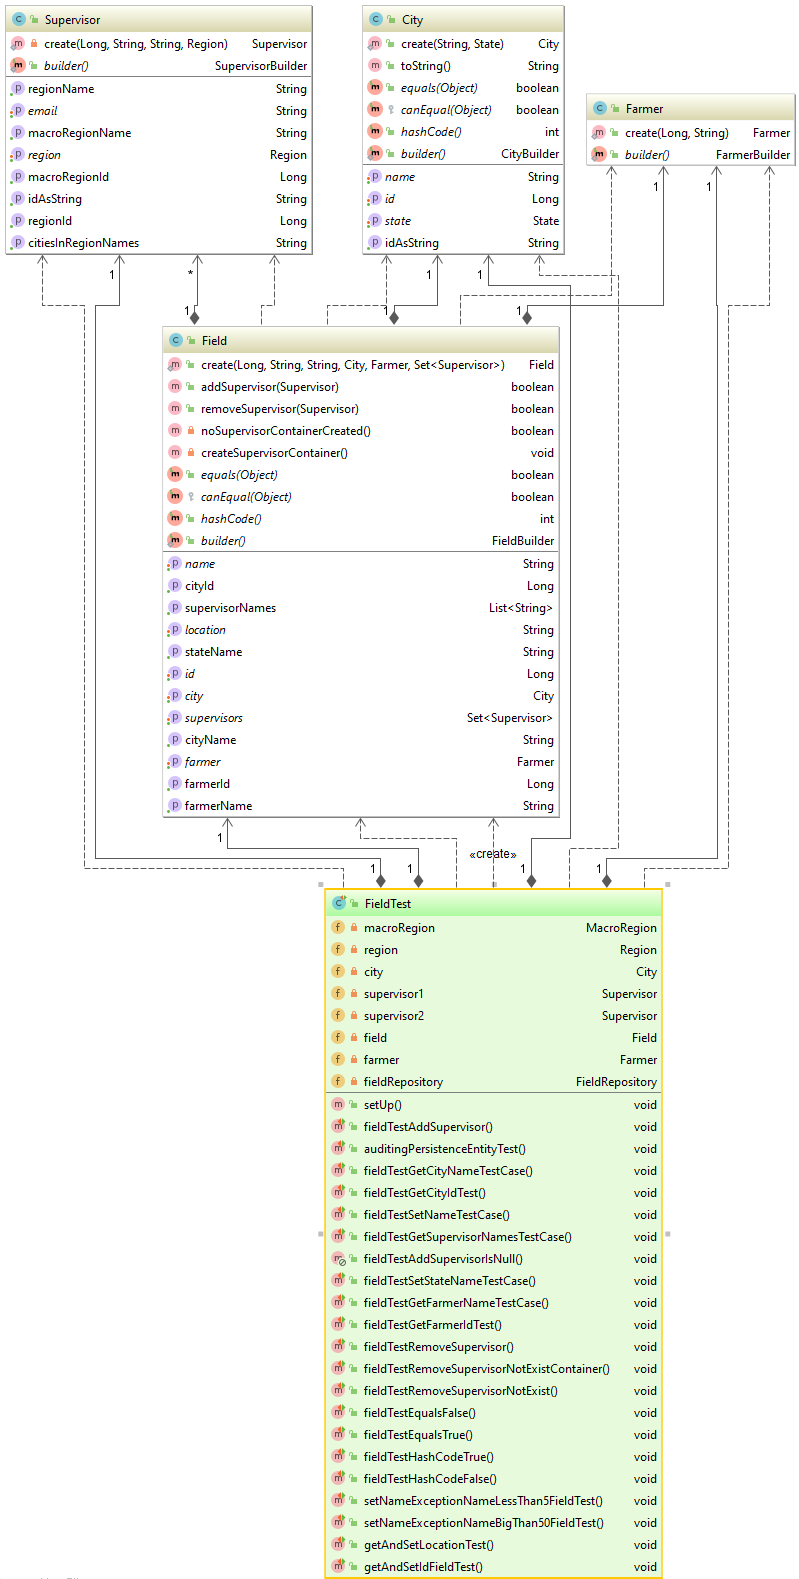
\includegraphics[scale=0.5]{dados/figuras/PackagebaseTestField.png}
	\caption{Diagrama de classes FieldServiceTest.java.}
	\label{packFieldService}
\end{figure}

A classe \textit{FieldService}é responsável por realizar a comunicação com a classe \textit{Field}, e com as demais classes que a compõem. A FIGURA \ref{packFieldService} apresenta o diagrama de classes da classe \textit{FieldService}e as demais classes que a compõem assim como a classe responsável por realizar os testes de seus métodos e variáveis. Também é possível analisar no diagrama os atributos e métodos que pertence à classe \textit{ FieldService }, assim como os métodos e atributos da classe de \textit{ FieldServiceTest}.  


A classe de teste apresentada na FIGURA \ref{packFieldService} possui vinte e três métodos de teste é um método de apoio aos testes denominado \textit{“setUp”}, o objetivo dos testes é exercitar a classe \textit{FieldService} até que todos as variáveis, entradas e saídas de dados sejam executados pelo menos uma vez. Como a classe \textit{FieldService} trabalha com outras classes além da \textit{Field} se faz necessário a instanciação destas como: \textit{Supervisor}, \textit{Farmer}, \textit{City} e outras para a execução completa dos testes. Como a classe trabalha com entidades que serão persistidas em um banco de dados, foi preciso criar uma referência para a interface \textit{FieldRepository} e outros repositórios que são chamados durante a execução dos testes. Como o objetivo deste trabalho é cobrir o sistema com testes unitários e testes que integram classes entidades com o banco de dados ou comunicação com APIs são testes de integração foi utilizado\textit{ “Mocks”} para simular o comportamento dos repositórios.



A FIGURA \ref{testeFieldService} apresenta a declaração da classe de teste, os atributos utilizados para desenvolver os testes e o método\textit{ “setUp”} utilizado para preparar o ambiente para os teste.

O trecho de código da FIGURA \ref{testeFieldService} apresenta as seguintes funcionalidades:

\begin{itemize}
\item Linha 1 A anotação \textit{@RunWith} permite a execução dos testes dentro de um contexto do \textit{Spring}. O comando \textit{SpringRunner}.class fornece suporte para carregar um \textit{Spring} \textit{ApplicationContext} e ter \textit{beans }\textit{@Autowired} na instância de teste.
\item Na linha 2 é utilizada a anotação \textit{@SpringBootTest} que prepara um contexto \textit{Spring} e inclui a possibilidade de iniciar um container em um porta default ou configurada pelo usuário. Neste caso a porta foi definida de forma randômica através do comando \textit{“SpringBootTest.WebEnvironment.RANDOM\_PORT”}; 

 \item Na linha 3 é utilizada a anotação \textit{@FixMethodOrder} que permite definir uma ordem de execução dos testes, neste casso foi definida a ordem \textit{“NAME\_ASCENDING"} que faz a execução dos testes de acordo com o nome de maneira ascendente;

 \item Linha 4 a classe \textit{FieldServiceTest} é aberta;

 \item Da linha 6 a 15 há a declaração dos objetos \textit{MOCKs} que serão utilizadas para a comunicação com o banco de dados. A anotação \textit{@MockBean} foi utilizada na declaração destas variáveis, ela permite que caso exista um \textit{bean }compatível com a classe declarada no contexto da aplicação \textit{Spring} este \textit{bean }será substituído por um \textit{Mock};

\item Linhas 14 e 15 uma instancia da classe \textit{FieldService}é declarada, a anotação \textit{@Autowired} é utilizada para a injeção automática de um \textit{bean }correspondente ao declarado na variável.
 
\item Da linha 17 a 21 há a declaração dos objetos que serão utilizados nos testes;

 



\item Na linha 24 é utilizado a anotação \textit{@Before}, esta anotação determina que sempre antes da execução de um teste o método \textit{“setUp”} deve ser executado primeiro.


\begin{figure}[H]
	\centering
	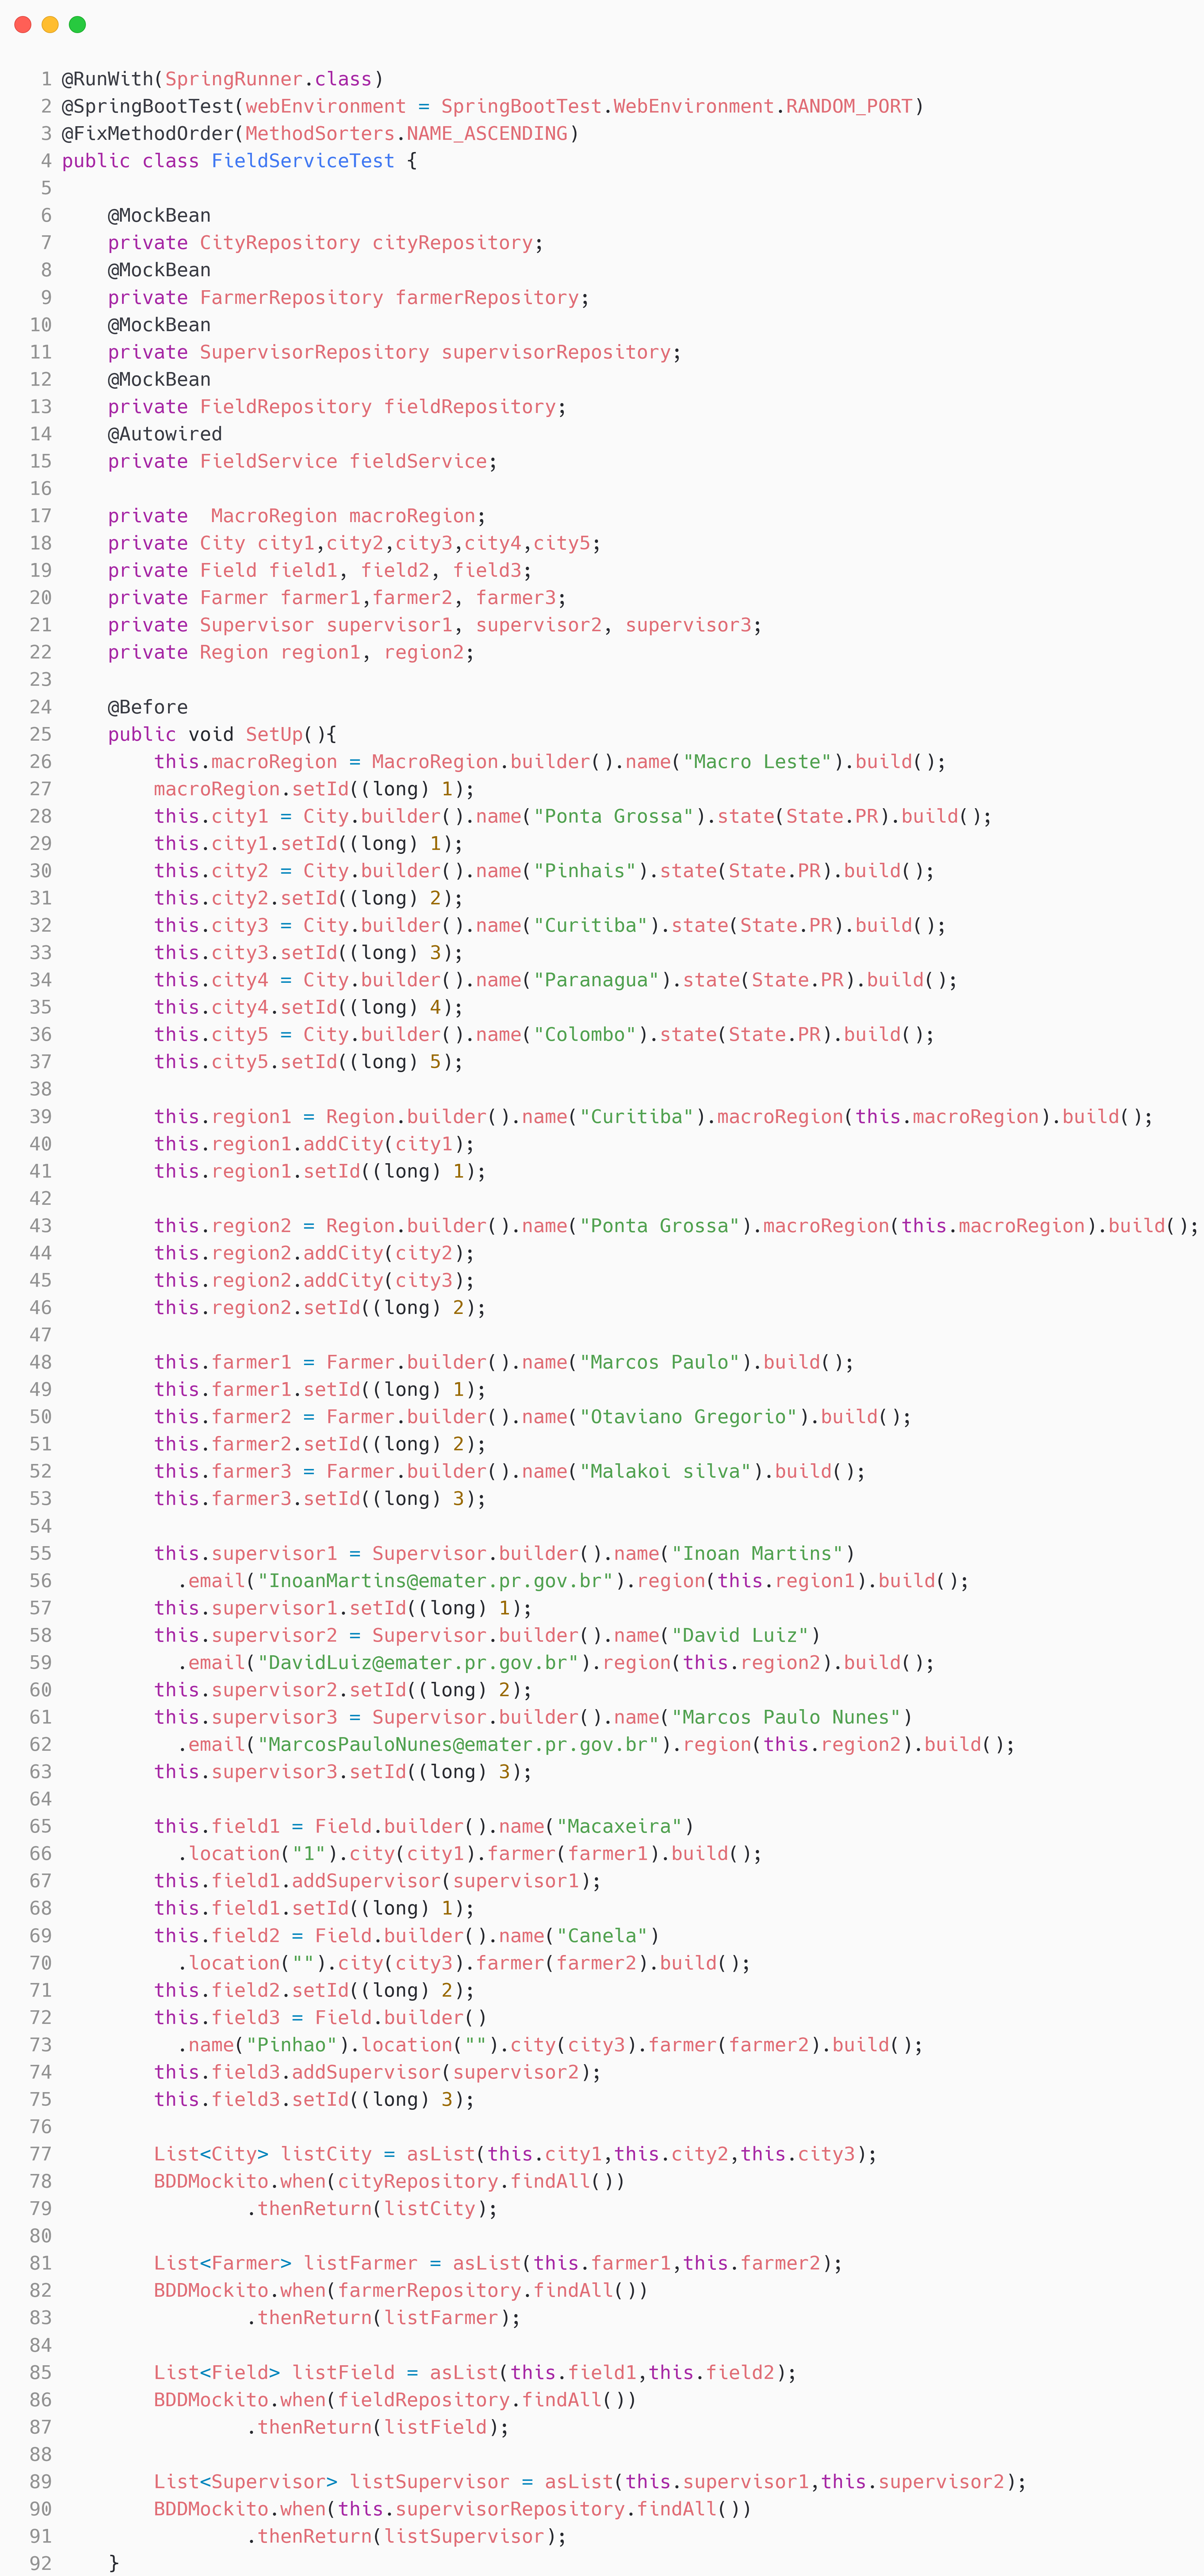
\includegraphics[scale=0.13]{dados/figuras/carbonFieldServicebuild.png}
\end{figure}

\begin{figure}[H]
	\centering
	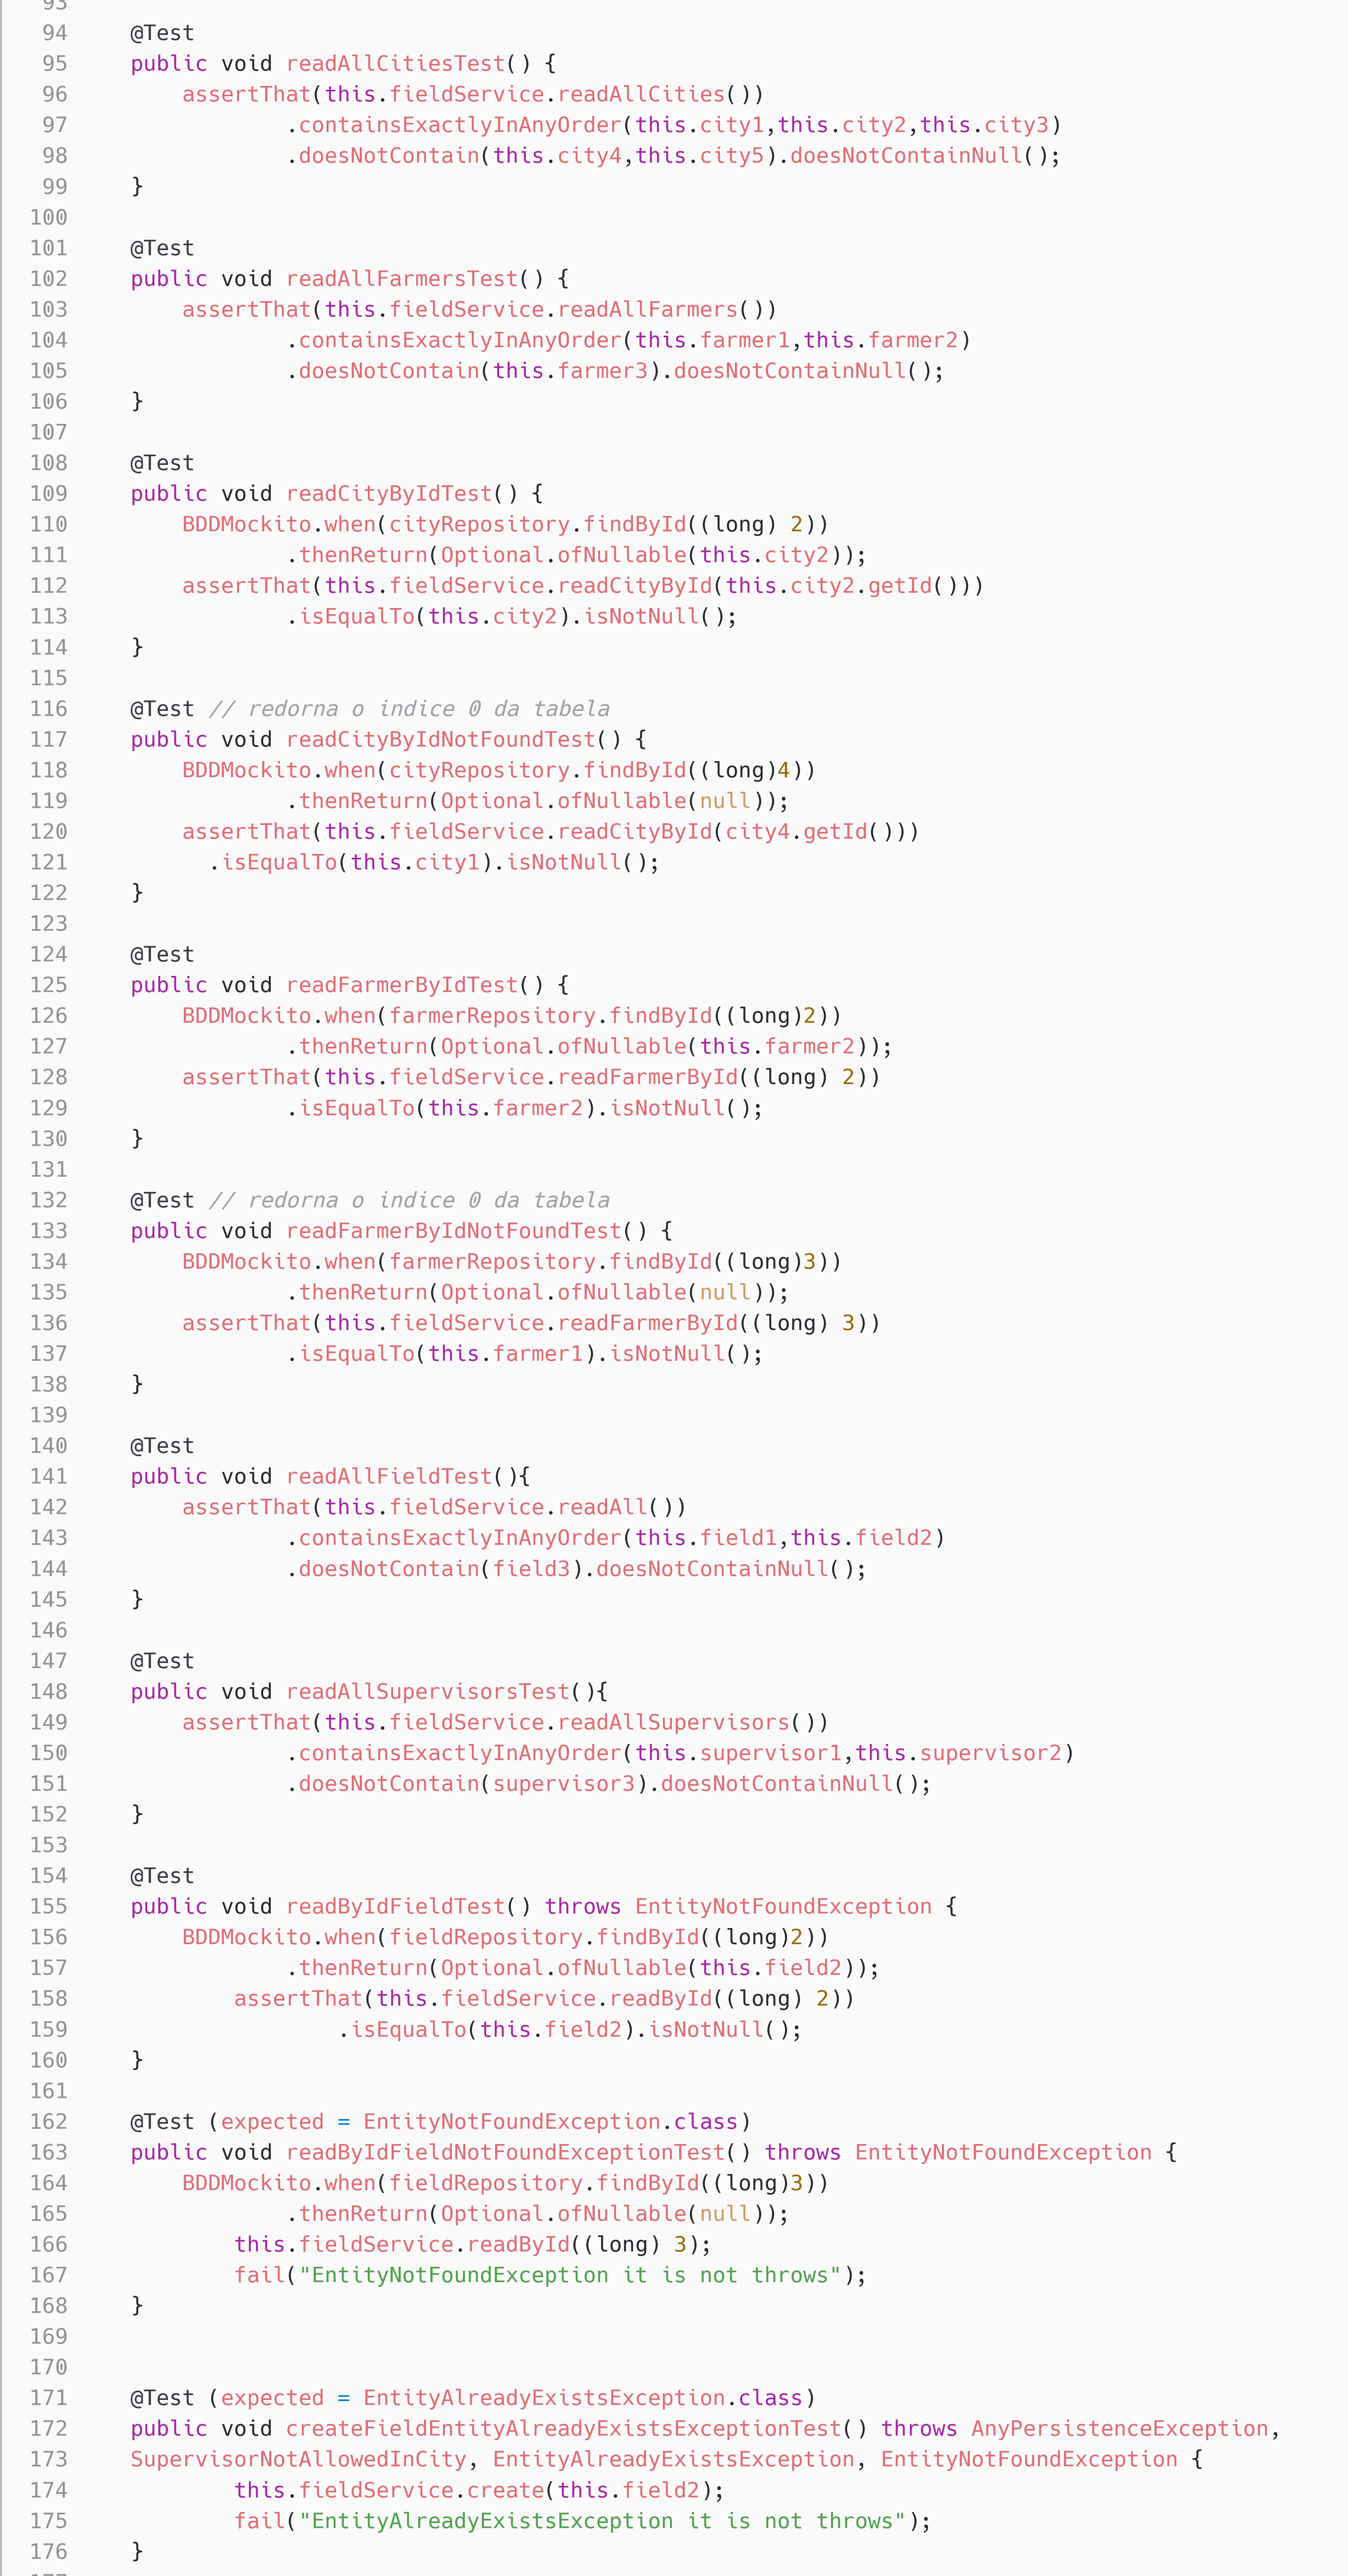
\includegraphics[scale=0.14]{dados/figuras/carbonFieldService1.png}
\end{figure}

\begin{figure}[H]
	\centering
	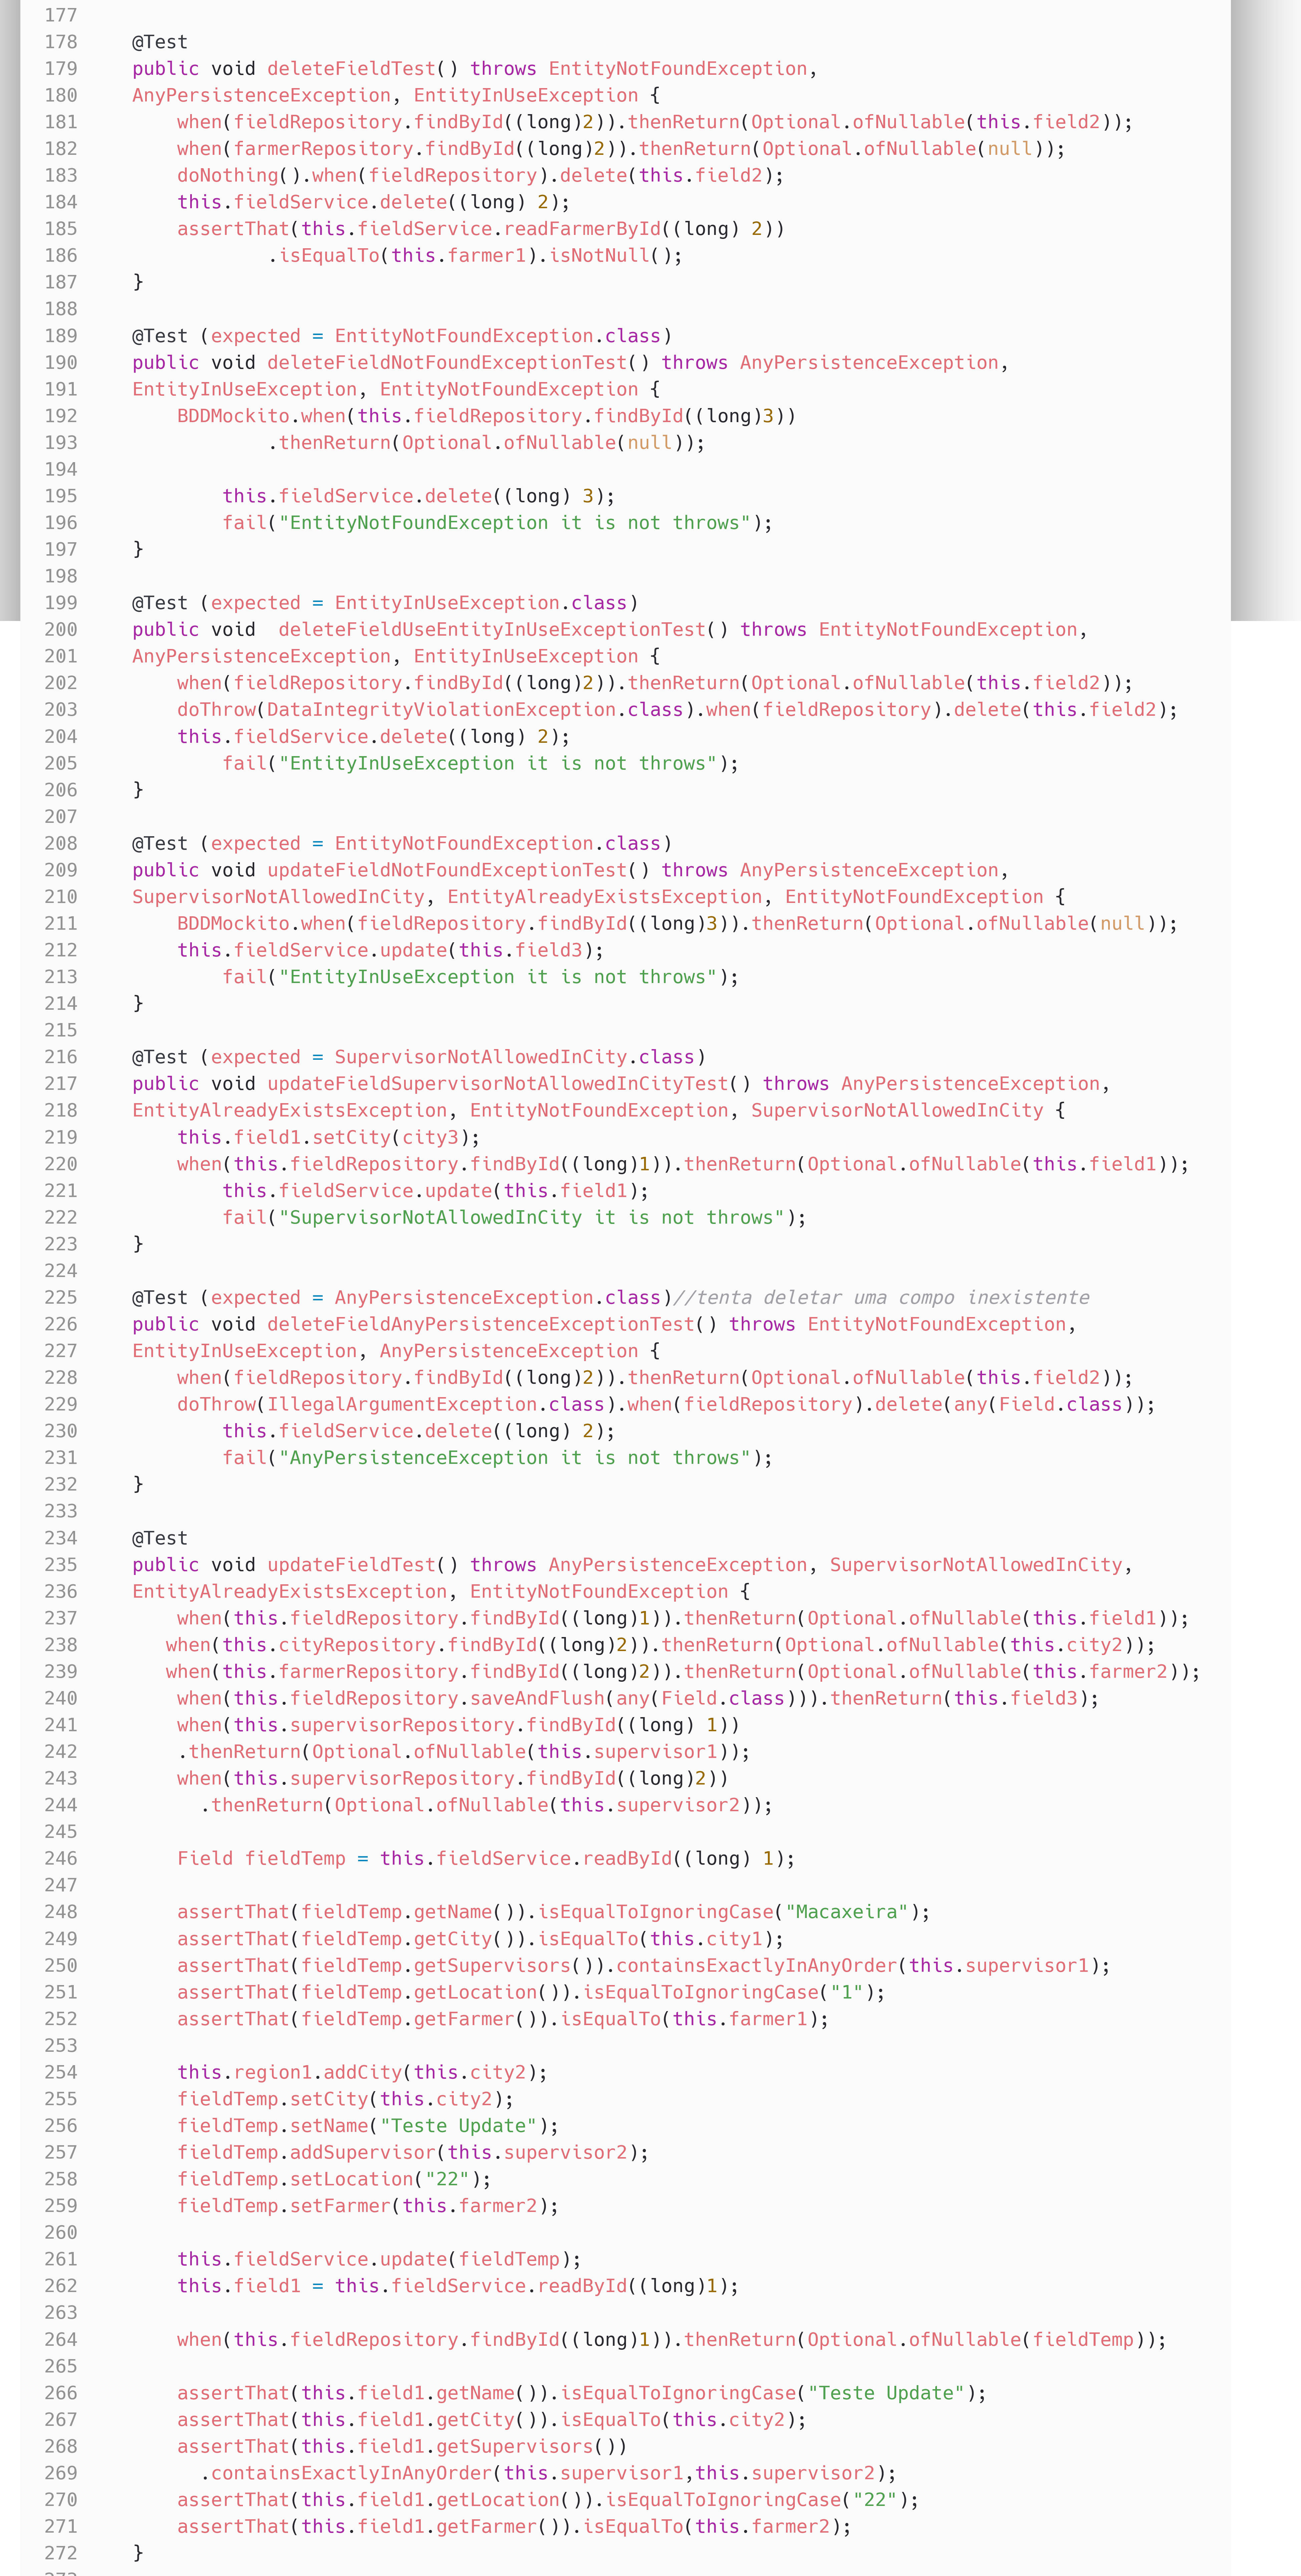
\includegraphics[scale=0.13]{dados/figuras/carbonFieldService2.png}
\end{figure}

\begin{figure}[H]
	\centering
	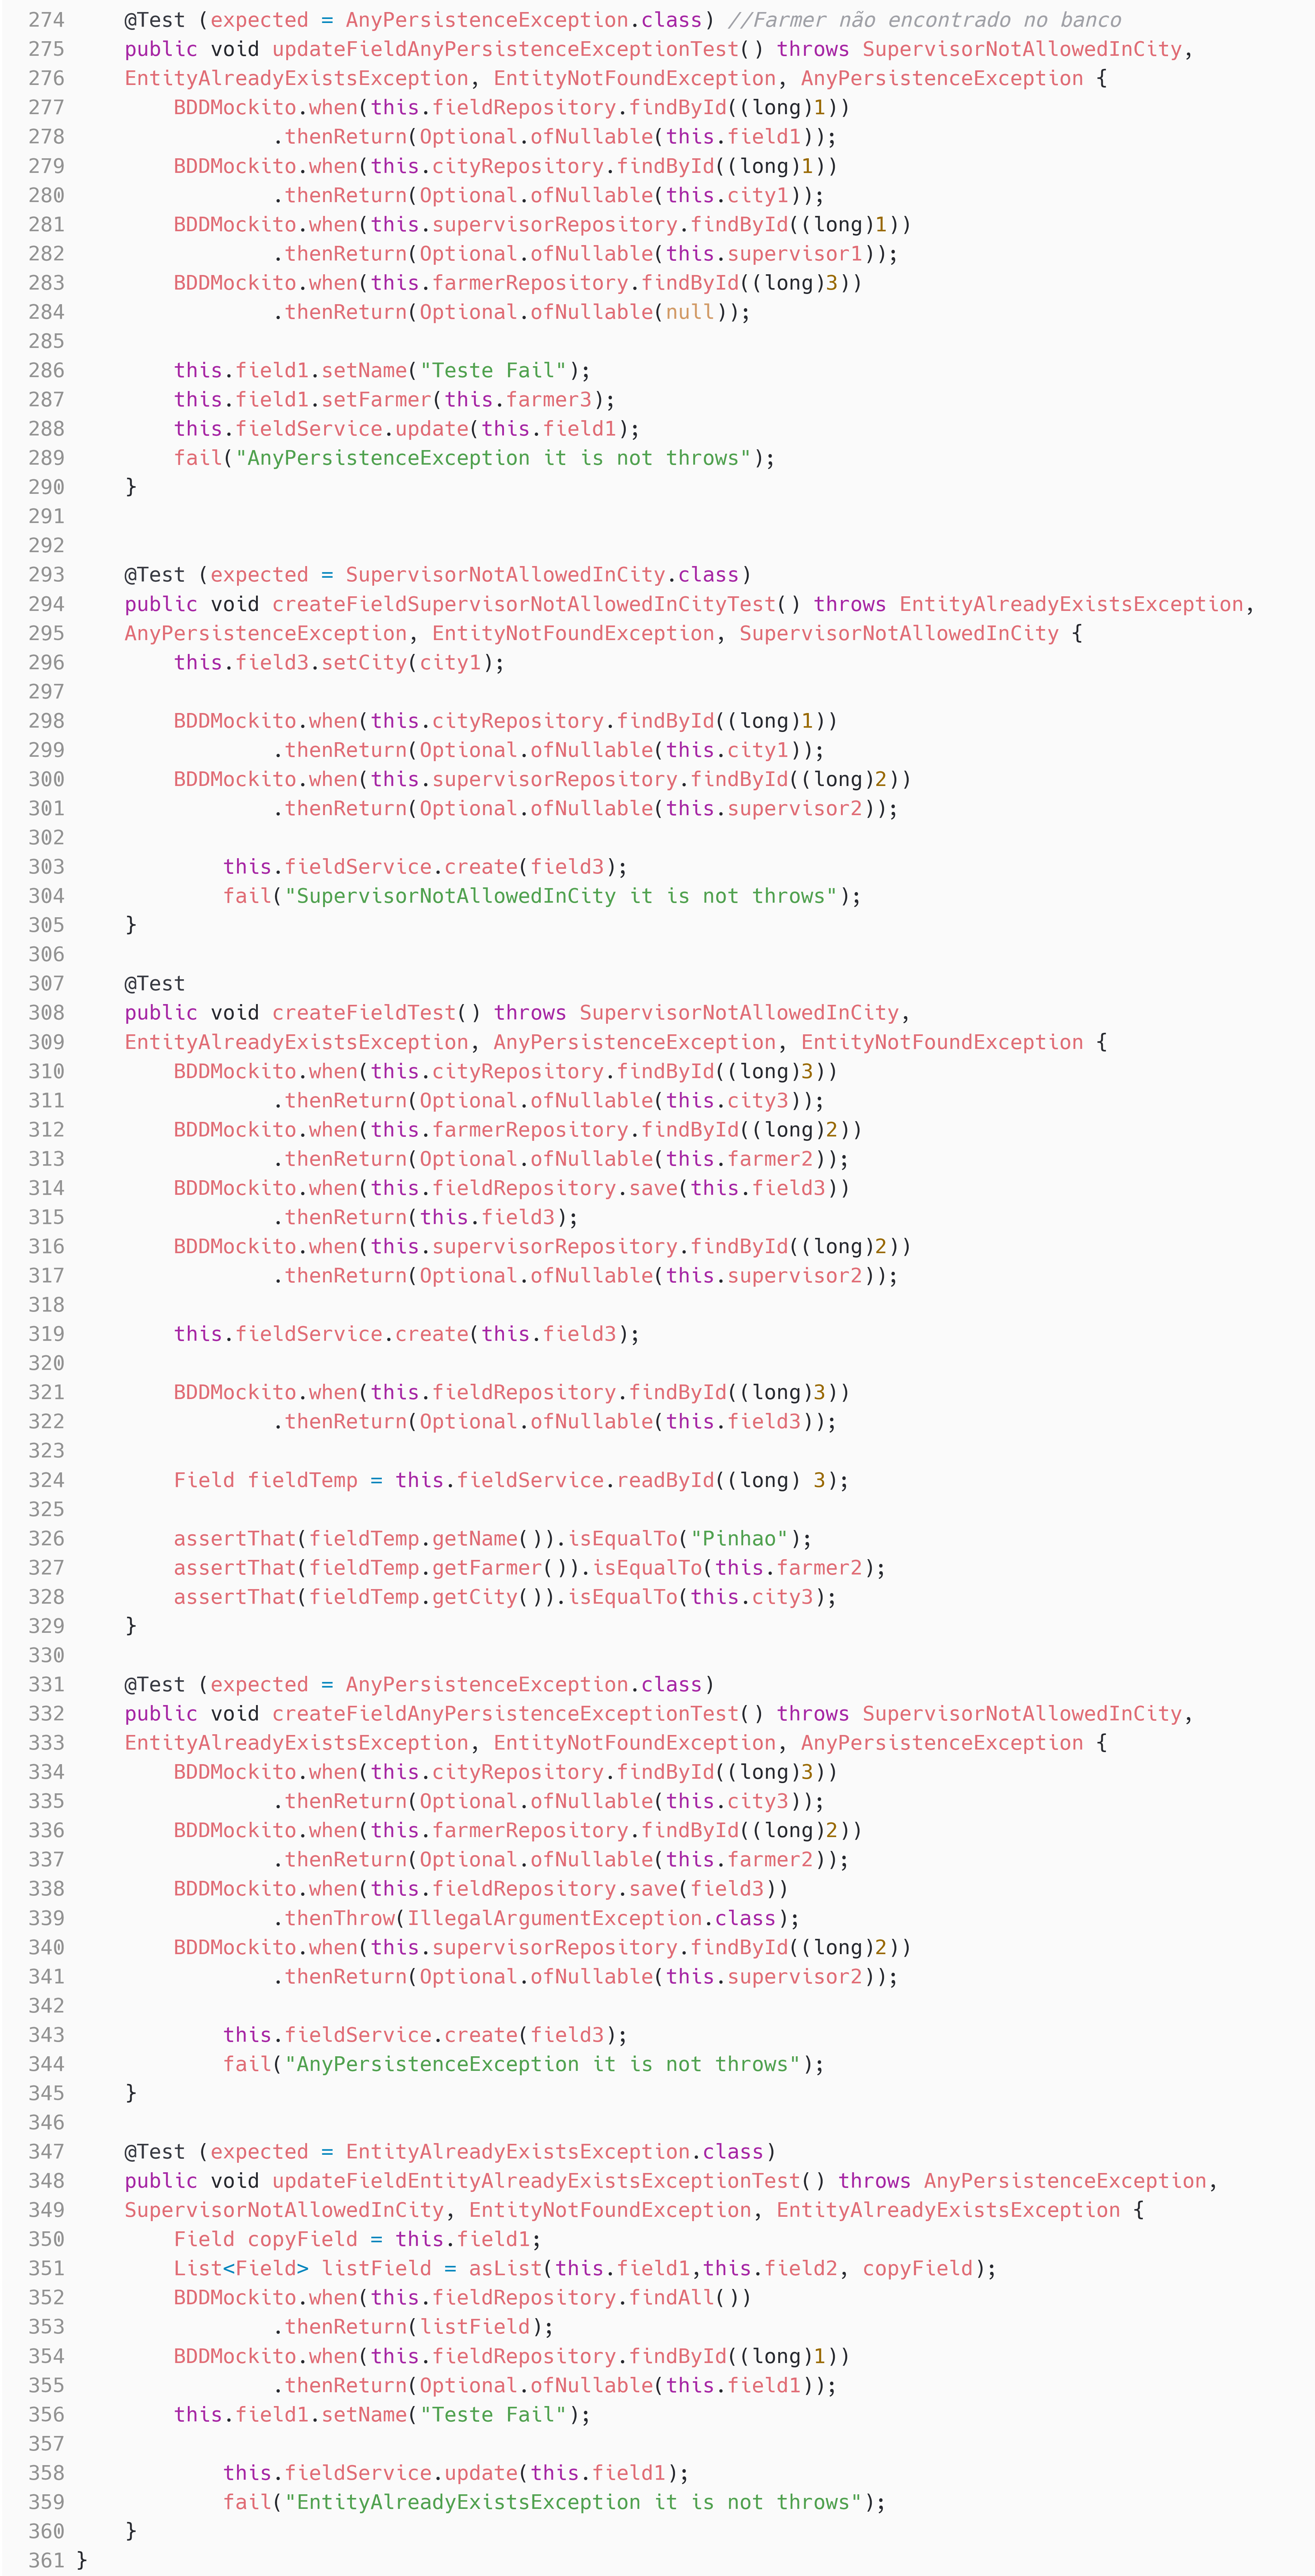
\includegraphics[scale=0.13]{dados/figuras/carbonFieldService3.png}
	\caption{Classe de Teste  FieldService.java.}
	\label{testeFieldService}
\end{figure}

 \item O método \textit{“setUp”} que tem sua declaração na linha 25 e vai até a linha 92 é responsável por realizar a construção dos objetos declarados nas linhas 17 a 21.

\item O método  \textit{“setUp”} também é responsável por construir algumas funcionalidades para os objetos do tipo Mock:

\begin{itemize}

 \item Linha  78 é definido que toda vez que o comando \textit{“cityRepository.findAll()”} for chamado o retorno será uma lista do tipo “\textit{City}” definida na linha 77;
\item Linha  82 é definido que toda vez que o comando \textit{“farmerRepository.findAll()”} for chamado o retorno será uma lista do tipo “\textit{Farmer}” definida na linha 81;
\item Linha  86 é definido que toda vez que o comando \textit{“fieldRepository.findAll()”} for chamado o retorno será uma lista do tipo \textit{Field} definida na linha 85;
\item Linha  90 é definido que toda vez que o comando\textit{ “supervisorRepository.findAll()”} for chamado o retorno será uma lista do tipo “\textit{City}” definida na linha 89;
\end{itemize}{}
\end{itemize}{}


A FIGURA \ref{testeFieldService} tambem apresenta os casos de testes criados para a classe \textit{FieldTest}. 


A ideia geral na elaboração dos testes é a de cobrir cada atribuição de dados, as entrada e saída de dados da classe \textit{FieldService}, buscando a cobertura de 100\% das linhas métodos e atributo da classe. Os resultados obtidos da execução dos testes foram listados a seguir:


Método de teste \textit{readAllCitiesTest ()} linhas 94 a 99 figura \ref{testeFieldService}: Este teste lista todas as cidades do banco de dados. Não há entrada de dados. A Saída é uma lista do tipo \textit{“City”} contendo as cidades salvas na base de dados. Nesta assertiva o método testado deve retornar a lista criada na linha 77, que contem 3 objetos do tipo cidade correspondentes a comparação.

Método de teste \textit{ readAllFarmersTest ()} linhas 101 a 106 figura \ref{testeFieldService}: Este teste lista todos os agricultores do banco de dados. Não há entrada de dados. A Saída é uma lista do tipo \textit{“Farmer”} contendo agricultores salvos na base de dados. Nesta assertiva o método testado deve retornar a lista criada na linha 81, que contem 2 objetos do tipo agricultor correspondentes a comparação.

Método de teste \textit{ readCityByIdTest ()} linhas 108 a 114 figura \ref{testeFieldService}: Este teste busca uma cidade na base de dados pelo seu identificador único. A entrada consiste em um numeral do tipo \textit{“Long”}. A saída é um objeto do tipo \textit{“City”}. Nesta assertiva o método testado deve retornar o registro \textit{mocado} nas linhas 110 e 111, o qual corresponde ao objeto comparado. 

Método de teste \textit{ readCityByIdNotFoundTest ()} linhas 116 a 122 figura \ref{testeFieldService}: Este teste busca uma cidade na base de dados pelo seu identificador único. A entrada consiste em um numeral do tipo \textit{“Long”}. A saída é um objeto do tipo \textit{“City”}. Nesta assertiva o método testado deve retornar o índice zero da lista criada na linha 77, o qual corresponde ao objeto comparado.

Método de teste \textit{ readFarmerByIdTest ()} linhas 124 a 130 figura \ref{testeFieldService}: Este teste busca um agricultor na base de dados pelo seu identificador único. A entrada consiste em um numeral do tipo \textit{“Long”}. A saída é um objeto do tipo \textit{“Farmer”}. Nesta assertiva o método testado deve retornar o registro \textit{mocado} nas linhas 126 e 127, o qual corresponde ao objeto comparado.

Método de teste \textit{ readFarmerByIdNotFoundTest ()} linhas 132 a 138 figura \ref{testeFieldService}: Este teste busca um agricultor na base de dados pelo seu identificador único. A entrada consiste em um numeral do tipo \textit{“Long”}. A saída é um objeto do tipo \textit{“Farmer”}. Nesta assertiva o método testado deve retornar o índice zero da lista criada na linha 81, o qual corresponde ao objeto comparado.


Método de teste \textit{ readAllFieldTest ()} linhas 140 a 145 figura \ref{testeFieldService}: Este teste busca os registros do tipo \textit{Field} na base de dados. Não há entrada de dados.  A saída é uma lista do tipo \textit{Field}. Nesta assertiva o método testado deve retornar a lista criada na linha 85, que contem dois registros correspondentes a comparação.

Método de teste \textit{readAllSupervisorsTest ()} linhas 147 a 152 figura \ref{testeFieldService}: Este teste busca os registros do tipo \textit{“Supervisor”} na base de dados. Não há entrada de dados.  A saída é uma lista do tipo \textit{“Supervisor”}. Nesta assertiva o método testado deve retornar a lista criada na linha 89, que contém dois registros correspondentes a comparação.

Método de teste \textit{ readByIdFieldTest ()} linhas 154 a 160 figura \ref{testeFieldService}: Este teste busca um registro do tipo \textit{Field} na base de dados pelo seu identificador único. A entrada consiste em um numeral do tipo \textit{“Long”}. A saída é um objeto do tipo \textit{Field}. Nesta assertiva o método testado deve retornar o objeto \textit{mocado} nas linhas 156 e 157, o qual corresponde ao objeto comparado.

Método de teste \textit{ readByIdFieldNotFoundExceptionTest ()} linhas 162 a 168 figura \ref{testeFieldService}: Este teste busca um registro do tipo \textit{Field} na base de dados pelo seu identificador único, quando não encontrado é gerada uma exceção. A entrada consiste em um numeral do tipo \textit{“Long”}. A saída é uma exceção do tipo \textit{“EntityNotFoundException”}. Nesta assertiva o método testado deve retornar uma exceção, ao buscar um objeto pelo índice passado como parâmetro, ao realizar a consulta no banco um registro vazio é retornado, o que é simulado nas linhas 164 e 165, o que garante o lançamento da exceção \textit{“EntityNotFoundException”}.


Método de teste \textit{ createFieldEntityAlreadyExistsExceptionTest ()} linhas 171 a 176 figura \ref{testeFieldService}:  Este teste consiste em tentar criar um novo registro do tipo \textit{Field}, mas o item a ser criado é identificado como já existente na base de dados. A Entrada consiste em um objeto do tipo \textit{Field}. A Saída é o lançamento da exceção \textit{“EntityAlreadyExistsException”}. A assertiva tenta inserir um registro que já se encontra na base de dados simulada pela linha 85, o que proporciona o lançamento da exceção.  

Método de teste \textit{ deleteFieldTest ()} linhas 178 a 187 figura \ref{testeFieldService}: Este teste consiste em deletar um registro do tipo \textit{Field}. A Entrada consiste em um objeto do tipo \textit{Field}. Não há saída de dados.  A assertiva deleta um registro do banco linha 183, a validação é feita ao tentar consultar por este registro no banco simulado, o retorno é o índice zero do banco e não o procurado.  

Método de teste \textit{ deleteFieldNotFoundExceptionTest ()} linhas 189 a 197 figura \ref{testeFieldService}: Este teste consiste em deletar um registro do tipo \textit{Field}, mas o item a ser deletado não existe na base de dados. A Entrada consiste em um objeto do tipo \textit{Field}. A Saída é o lançamento da exceção \textit{“EntityNotFoundException”}. A assertiva tenta deletar um registro, mas ao consultar o registro na base de dados simulada pela linha 192 o retorno é um nulo pois ele não existe na base, há o lançamento da exceção.  

Método de teste \textit{ deleteFieldUseEntityInUseExceptionTest ()} linhas 199 a 206 figura \ref{testeFieldService}: Este teste consiste em deletar um registro do tipo \textit{Field}, mas o item a ser deletado está sendo utilizado na base de dados. A Entrada consiste em um objeto do tipo \textit{Field}. A Saída é o lançamento da exceção \textit{“UseEntityInUseException”}. A assertiva tenta deletar um registro, mas este está sendo utilizado na base de dados simulada pela linha 203, há o lançamento da exceção.  

Método de teste \textit{ updateFieldNotFoundExceptionTest ()} linhas 208 a 214 figura \ref{testeFieldService}: Este teste consiste em atualizar um registro do tipo \textit{Field}, mas o item a ser atualizado não existe na base de dados. A Entrada consiste em um objeto do tipo \textit{Field}. A Saída é o lançamento da exceção \textit{“EntityNotFoundException”}. A assertiva tenta atualizar um registro, mas ao consultar o registro na base de dados simulada pela linha 211 o retorno é um nulo pois ele não existe na base, há o lançamento da exceção.  

Método de teste \textit{ updateFieldSupervisorNotAllowedInCityTest ()} linhas 216 a 223 figura \ref{testeFieldService}: Este teste consiste em tentar atualizar um registro do tipo \textit{Field}, mas é identificado que os supervisores presentes no registro não pertencem a cidade que compõe o registro. A Entrada consiste em um objeto do tipo \textit{Field}. A Saída é o lançamento da exceção \textit{“SupervisorNotAllowedInCity”}. A assertiva tenta atualizar um registro que possui supervisores que não se localizam na cidade do registro linha 219, o que proporciona o lançamento da exceção.  


Método de teste \textit{ deleteFieldAnyPersistenceExceptionTest ()} linhas 225 a 232 figura \ref{testeFieldService}: Este teste consiste em deletar um registro do tipo \textit{Field}, mas o item a ser deletado gera um erro na base de dados. A Entrada consiste em um objeto do tipo \textit{Field}. A Saída é o lançamento da exceção \textit{“AnyPersistenceException”}. A assertiva tenta deletar um registro, mas um erro é gerado, há o lançamento da exceção.  

Método de teste \textit{ updateFieldTest ()} linhas 234 a 272 figura \ref{testeFieldService}: Este teste consiste em atualizar um registro do tipo \textit{Field}. A Entrada consiste em um objeto do tipo \textit{Field}. Não há saída de dados. As assertivas consistem em recuperar um objeto da base de dados simulada linha 237, atualizar os campos deste objeto linhas 254 a 259, e em seguida atualizar esse registro na base linha 240. Caso não haja o lançamento de uma exceção o objeto atualizado é recuperado da base simulada, linha 264, e em seguida é feita as assertivas dos dados atualizados.

Método de teste \textit{ updateFieldAnyPersistenceExceptionTest ()} linhas 274 a 290 figura \ref{testeFieldService}: Este teste consiste em atualizar um registro do tipo \textit{Field}, mas o item a ser atualizado possui um agricultor nulo. A Entrada consiste em um objeto do tipo \textit{Field}. A Saída é o lançamento da exceção \textit{“AnyPersistenceException”}. A assertiva tenta atualizar um registro, mas ao consultar o agricultor na base de dados simulada pela linha 283 o retorno é um nulo, há o lançamento da exceção.  

Método de teste \textit{ createFieldSupervisorNotAllowedInCityTest ()} linhas 293 a 305 figura \ref{testeFieldService}: Este teste consiste em tentar criar um novo registro do tipo \textit{Field}, mas é identificado que os supervisores presentes no registro não pertencem a cidade que compõe o registro. A Entrada consiste em um objeto do tipo \textit{Field}. A Saída é o lançamento da exceção \textit{“SupervisorNotAllowedInCity”}. A assertiva tenta inserir um registro que possui supervisores que não se localizam na cidade do registro linha 296, o que proporciona o lançamento da exceção.  

Método de teste \textit{ createFieldTest ()} linhas 307 a 329 figura \ref{testeFieldService}: Este teste consiste em criar um novo registro do tipo \textit{Field} na base de dados. A Entrada consiste em um objeto do tipo \textit{Field}. O método não gera uma saída. A validação é feita através de um \textit{try cath}, que captura qualquer exceção que ocorra ao salvar o objeto. Como o método não lança uma exceção ele é aceito. A assertiva, no entanto, é feita através do repositório \textit{mocado} linhas 321 e 322, depois de inserido é simulada uma consulta pelo identificador único do objeto inserido anteriormente o qual deve retornar o objeto que acaba de ser inserido. 

Método de teste \textit{ createFieldAnyPersistenceExceptionTest ()} linhas 331 a 345 figura \ref{testeFieldService}: Este teste consiste em tentar criar um novo registro do tipo \textit{Field}, mas o item a ser criado gera algum erro na base de dados. A Entrada consiste em um objeto do tipo \textit{Field}. A Saída é o lançamento da exceção \textit{“AnyPersistenceException”}. A assertiva tenta inserir um registro na base de dados simulada pela linha 338, o que proporciona o lançamento da exceção.  

Método de teste \textit{ updateFieldEntityAlreadyExistsExceptionTest ()} linhas 347 a 360 figura \ref{testeFieldService}: Este teste consiste em tentar atualizar um registro do tipo \textit{Field}, mas o item a ser atualizado é identificado como já existente na base de dados. A Entrada consiste em um objeto do tipo \textit{Field}. A Saída é o lançamento da exceção \textit{“EntityAlreadyExistsException”}. A assertiva tenta inserir um registro que já se encontra na base de dados simulada pela linha 351, neste caso foi necessário duplicar o registro a ser atualizado para que o lançamento da exceção fosse forçado.  

Após a execução dos testes a cobertura das entradas e saídas de dados da classe FieldService.java é de 100\%.


 \subsection{RESULTADO DOS TESTES CLASSE SURVEYSERVICE.JAVA}

A classe \textit{SurveyService} é responsável por realizar a comunicação com a classe \textit{Survey}, e com as demais classes que a compõem. A FIGURA \ref{packFieldService} apresenta o diagrama de classes da classe \textit{SurveyService} e as demais classes que a compõem assim como a classe responsável por realizar os testes de seus métodos e variáveis. Também é possível analisar no diagrama os atributos e métodos que pertence à classe \textit{SurveyService}, assim como os métodos e atributos da classe de \textit{SurveyServiceTest}.  


A classe de teste apresentada na FIGURA \ref{packFieldService} possui vinte e quatro métodos de teste é um método de apoio aos testes denominado \textit{“setUp”}, o objetivo dos testes é exercitar a classe \textit{SurveyService} até que todos as variáveis, entradas e saídas de dados sejam executados pelo menos uma vez. Como a classe \textit{SurveyService} trabalha com outras classes além da \textit{Survey} se faz necessário a instanciação destas como: \textit{Supervisor}, \textit{Farmer}, \textit{City} e outras para a execução completa dos testes. Como a classe trabalha com entidades que serão persistidas em um banco de dados, foi preciso criar uma referência para a interface \textit{SurveyRepository} e outros repositórios que são chamados durante a execução dos testes. Como o objetivo deste trabalho é cobrir o sistema com testes unitários e testes que integram classes entidades com o banco de dados ou comunicação com APIs são testes de integração foi utilizado “\textit{MOCKs}” para simular o comportamento dos repositórios.

 \begin{figure}[H]
	\centering
	\includegraphics[scale=0.4]{dados/figuras/PackagesurveyService.png}
	\caption{Diagrama de classes SurveyServiceTest.java.}
	\label{packFieldService}
\end{figure}


A FIGURA \ref{testeSurveyService} apresenta a declaração da classe de teste, os atributos utilizados para desenvolver os testes e o método\textit{ “setUp”} utilizado para preparar o ambiente para os testes.

O trecho de código da FIGURA \ref{testeSurveyService} apresenta as seguintes funcionalidades:


\begin{itemize}

\item Linha 1 A anotação \textit{@RunWith} permite a execução dos testes dentro de um contexto do \textit{Spring}. O comando \textit{SpringRunner}.class fornece suporte para carregar um \textit{Spring}\textit{ApplicationContext} e ter \textit{beans }\textit{@Autowired} na instância de teste.

\item Na linha 2 é utilizada a anotação \textit{@SpringBootTest} que prepara um contexto \textit{Spring} e inclui a possibilidade de iniciar um container em um porta default ou configurada pelo usuário. Neste caso a porta foi definida de forma randômica através do comando \textit{“SpringBootTest.WebEnvironment.RANDOM\_PORT”}; 

 \item Na linha 3 é utilizada a anotação \textit{@FixMethodOrder} que permite definir uma ordem de execução dos testes, neste casso foi definida a ordem \textit{“NAME\_ASCENDING"} que faz a execução dos testes de acordo com o nome de maneira ascendente;

 \item Linha 4 a classe \textit{SurveyServiceTest} é aberta;

 \item Da linha 6 a 11 há a declaração dos objetos \textit{MOCKs} que serão utilizadas para a comunicação com o banco de dados. A anotação \textit{@MockBean} foi utilizada na declaração destas variáveis, ela permite que caso exista um \textit{bean }compatível com a classe declarada no contexto da aplicação \textit{Spring} este \textit{bean }será substituído por um \textit{Mock};

\item Linhas 13 e 14 uma instancia da classe SurveyService é declarada, a anotação \textit{@Autowired} é utilizada para a injeção automática de um \textit{bean }correspondente ao declarado na variável. 
 
\item Da linha 16 a 21 há a declaração dos objetos que serão utilizados nos testes;

 \item Na linha 23 é utilizado a anotação \textit{@Before}, esta anotação determina que sempre antes da execução de um teste o método \textit{“setUp”} deve ser executado primeiro.

 \item O método \textit{“setUp”} que tem sua declaração na linha 24 e vai até a linha 108 é responsável por realizar a construção dos objetos declarados nas linhas 16 a 21.

\item O método  \textit{“setUp”} também é responsável por construir algumas funcionalidades para os objetos do tipo \textit{Mock}:

\begin{itemize}

 \item Linha  107 é definido que toda vez que o comando \textit{“surveyRepository.findAll()”} for chamado o retorno será uma lista do tipo “\textit{Survey}” definida na linha 106;
\end{itemize}{}
\end{itemize}{}


A FIGURA \ref{testeSurveyService} também apresenta os casos de testes criados para a classe \textit{SurveyService}. 


A ideia geral na elaboração dos testes é a de cobrir cada atribuição de dados, as entradas e saída de dados da classe \textit{ SurveyService}, buscando a cobertura de 100\% das linhas métodos e atributo da classe. Os resultados obtidos da execução dos testes foram listados a seguir:


Método de teste \textit{ readAllSurveyTest()} linhas 110 a 115 figura \ref{testeSurveyService}: Este teste lista todas as pesquisas do banco de dados. Não há entrada de dados. A Saída é uma lista do tipo \textit{“Survey”} contendo as pesquisas salvas na base de dados. Nesta assertiva o método testado deve retornar a lista criada na linha 106, que contem 2 objetos do tipo survey correspondentes a comparação.


\begin{figure}[H]
	\centering
	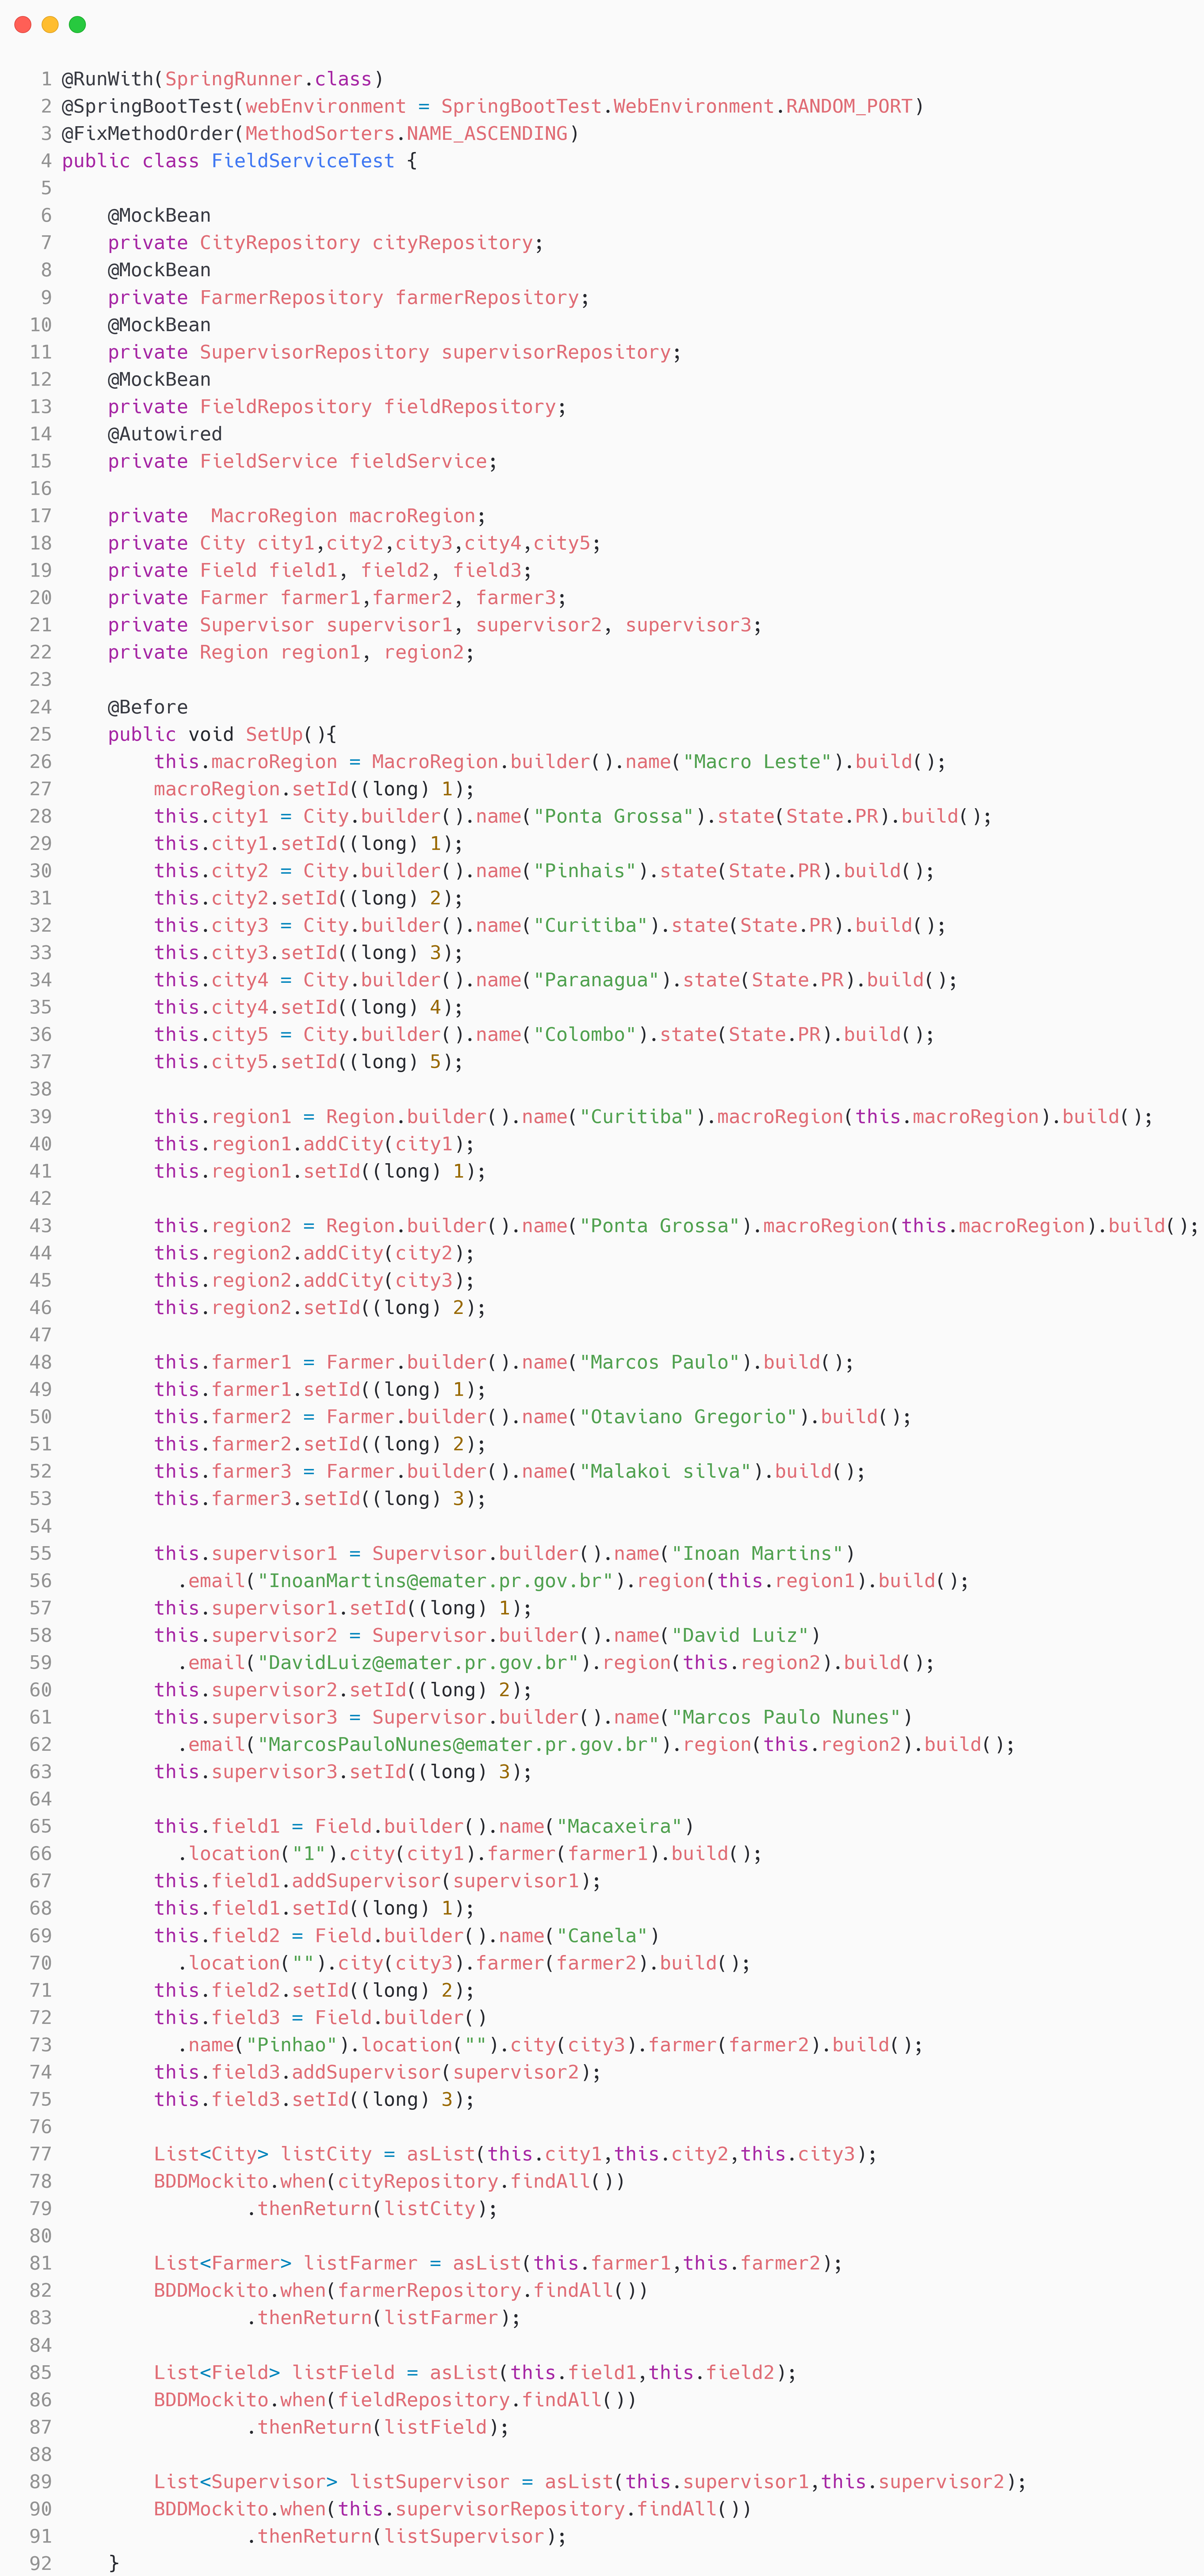
\includegraphics[scale=0.13]{dados/figuras/carbonFieldServicebuild.png}
\end{figure}

\begin{figure}[H]
	\centering
	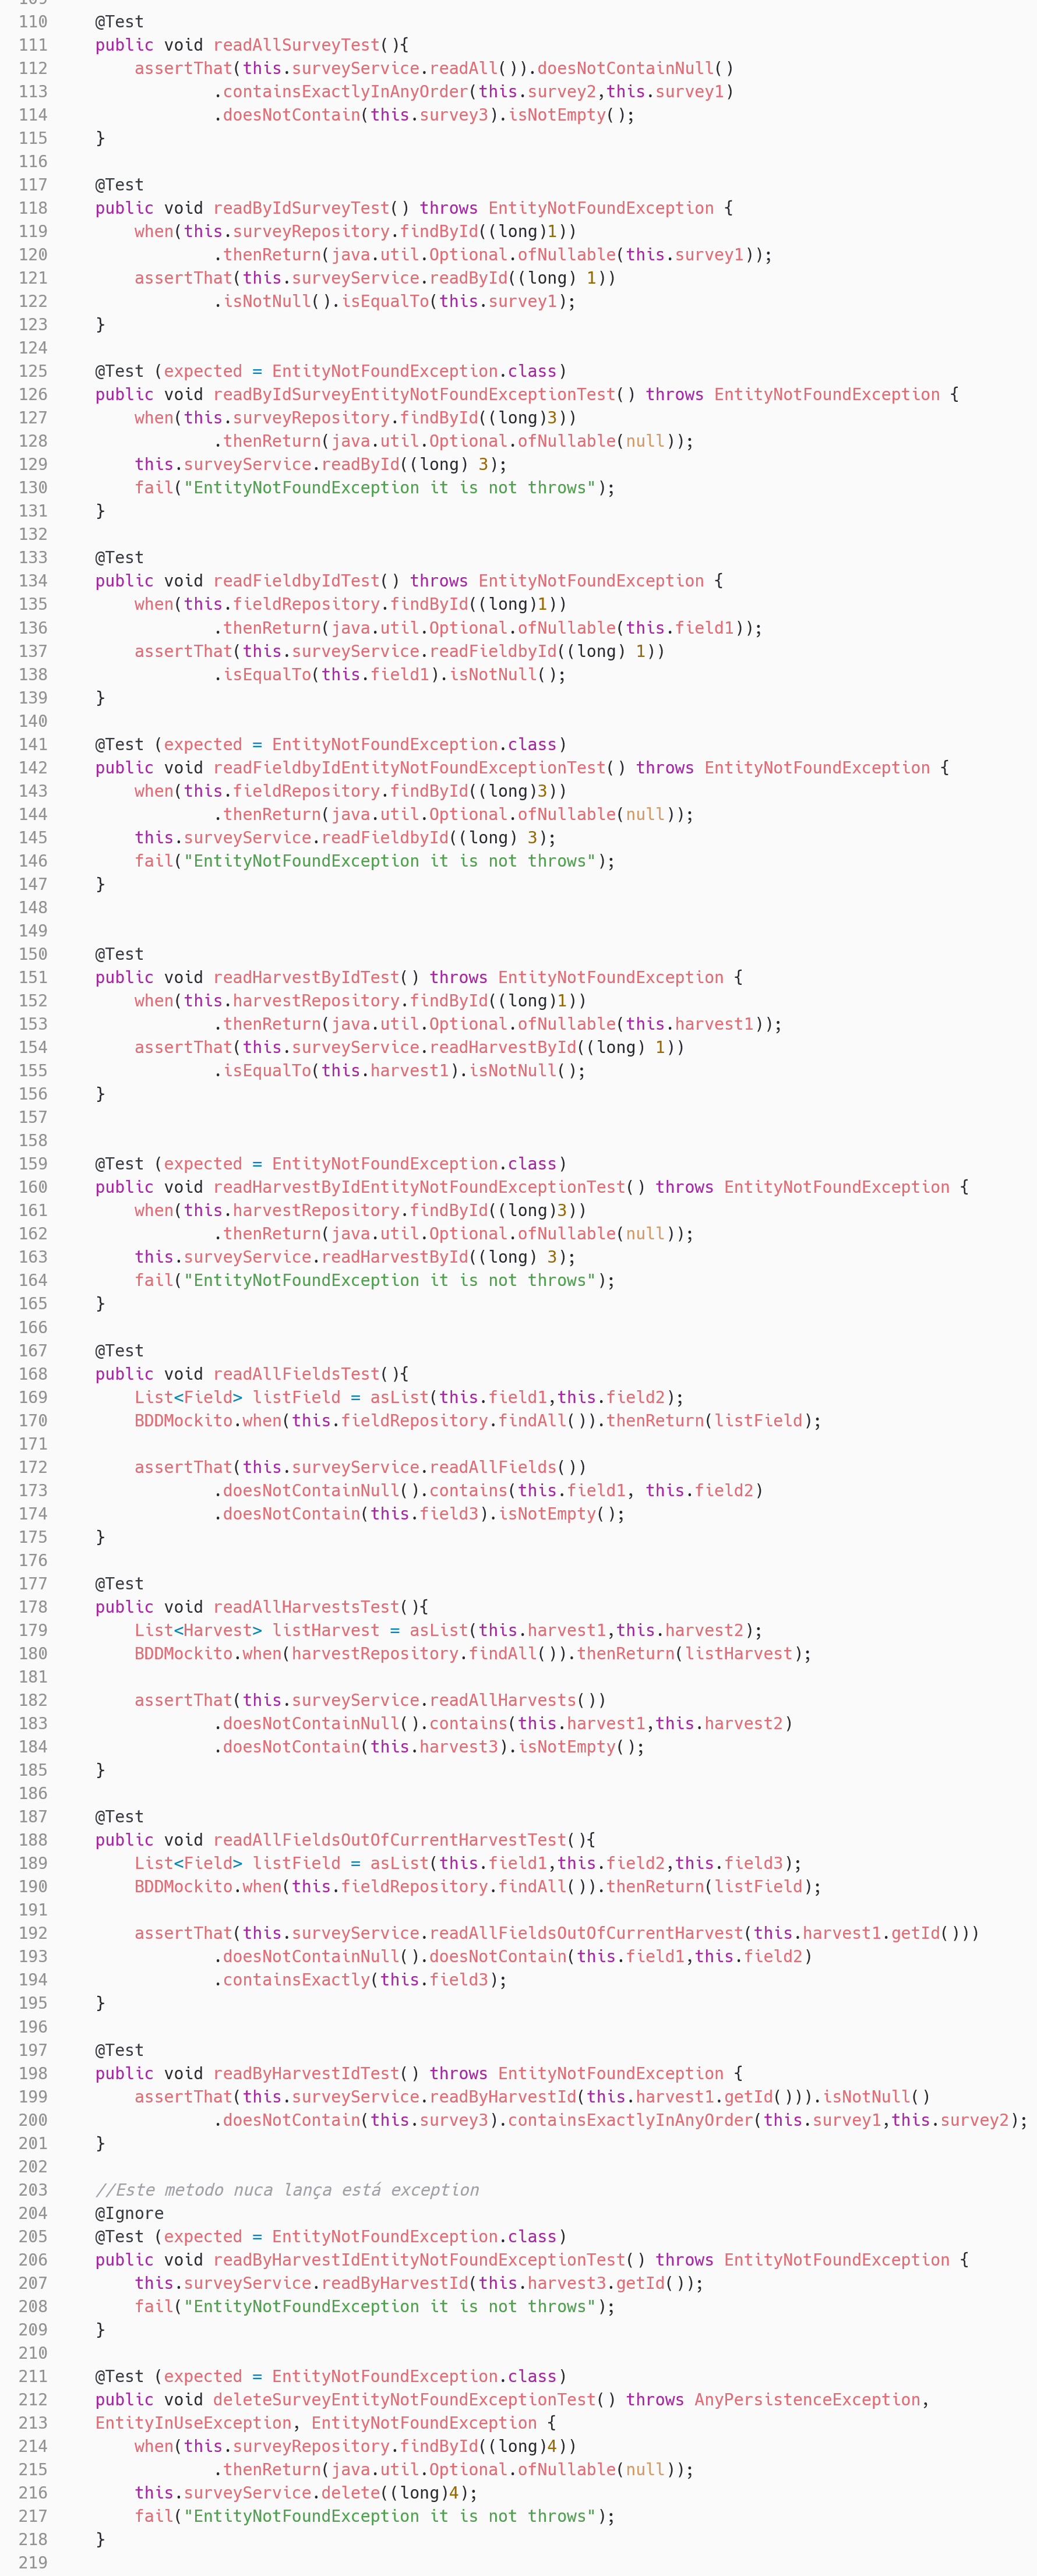
\includegraphics[scale=0.25]{dados/figuras/carbonSurveyService1.png}
\end{figure}

\begin{figure}[H]
	\centering
	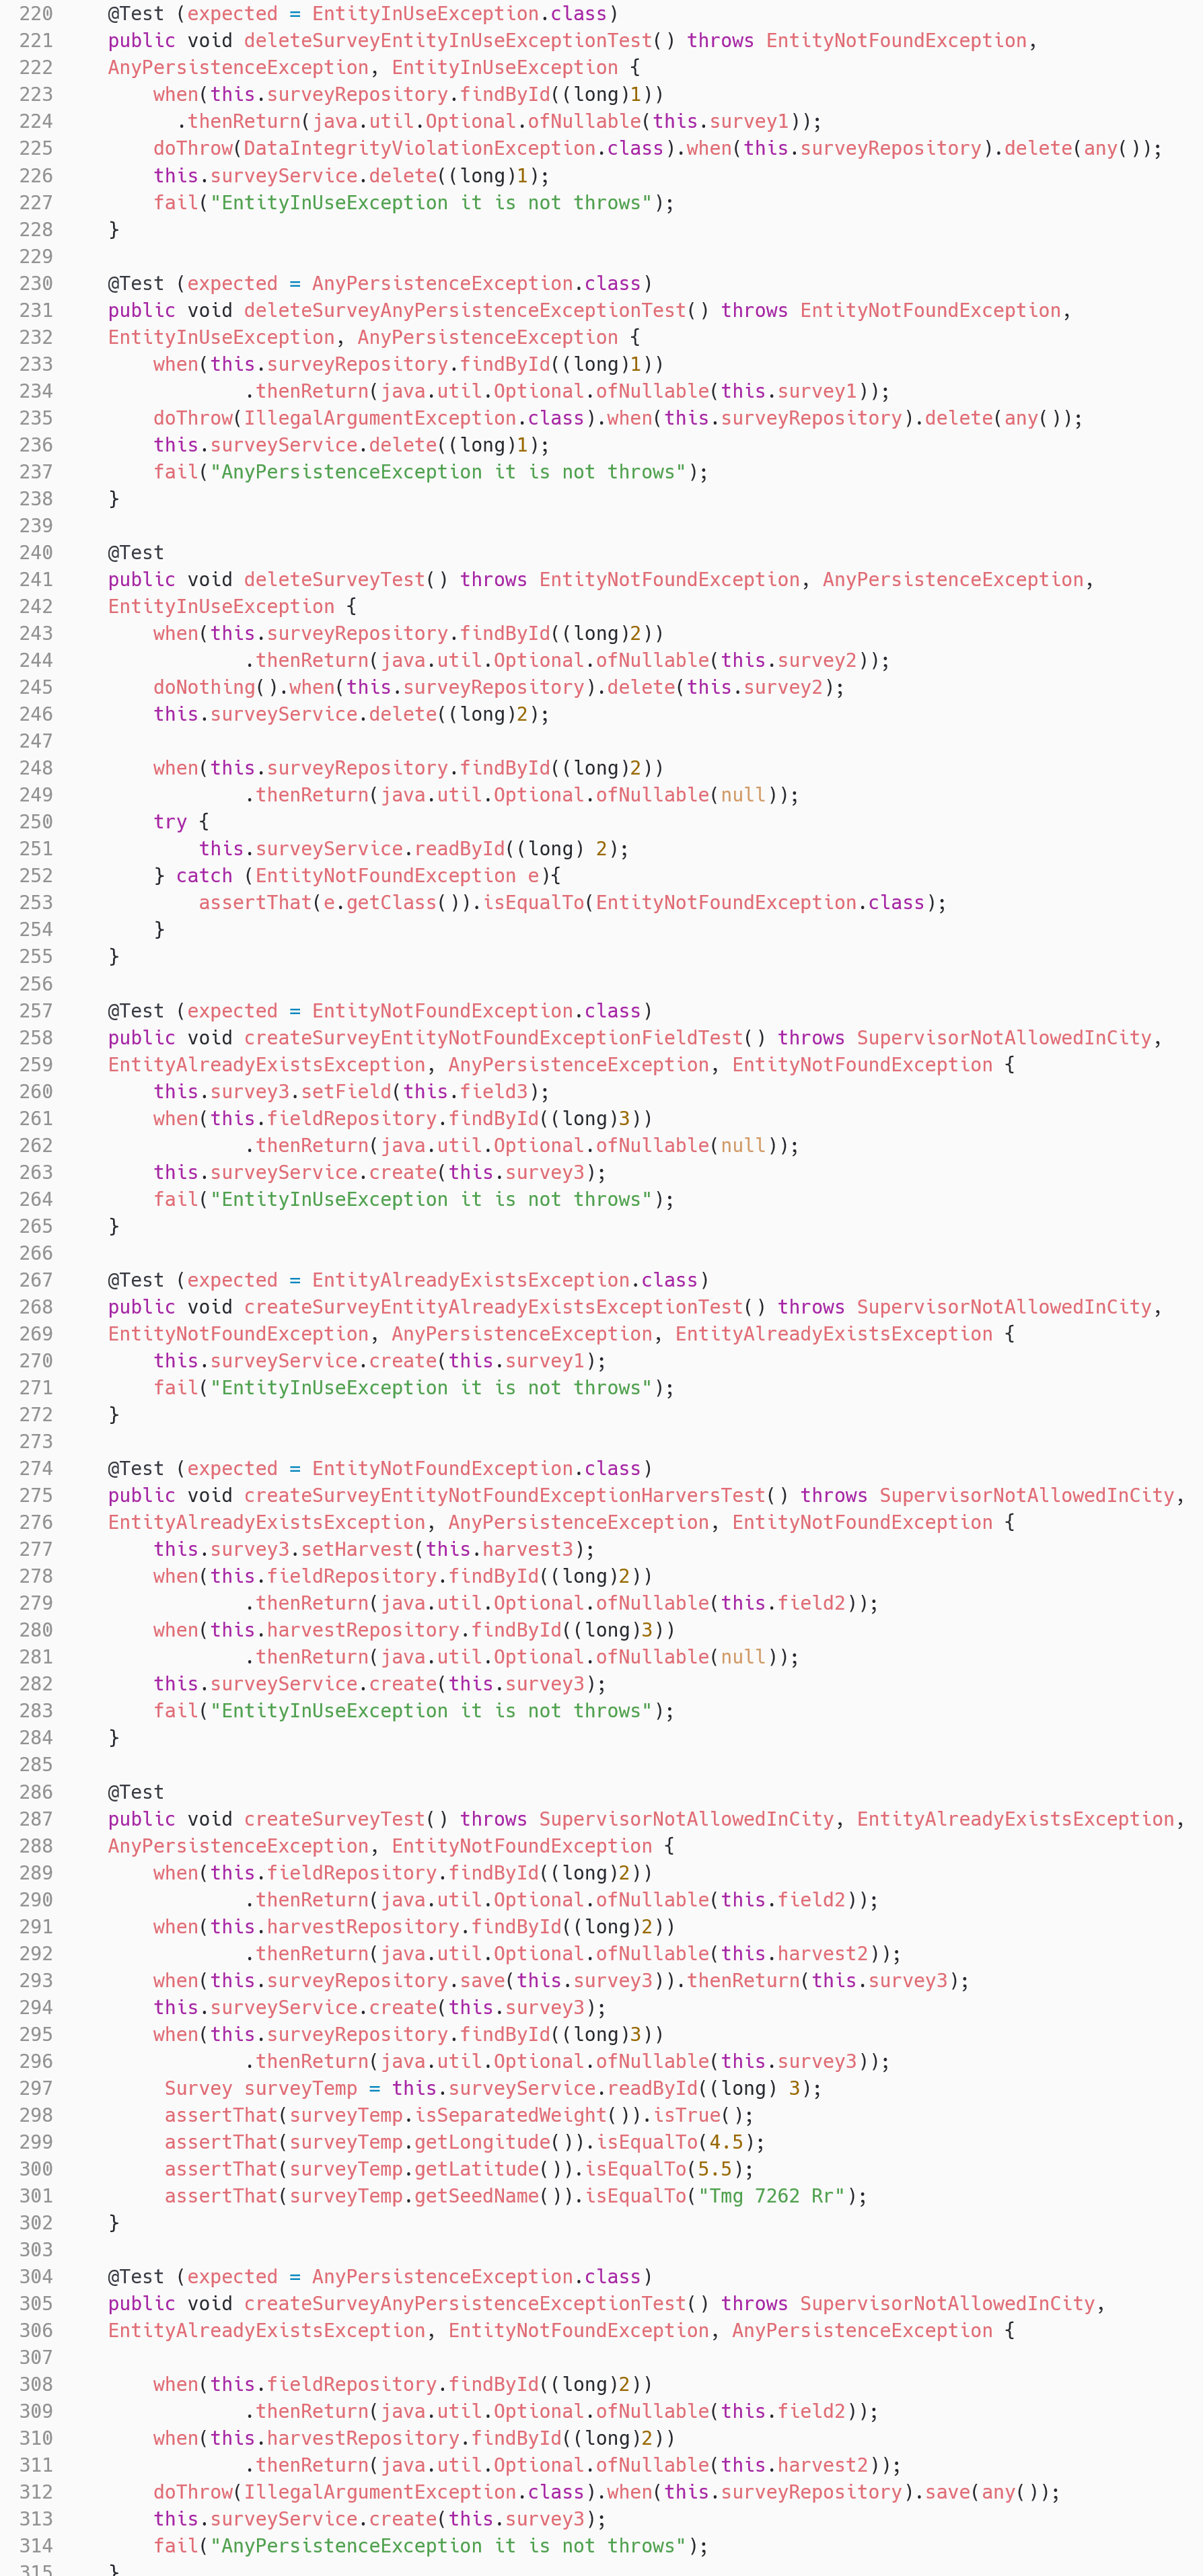
\includegraphics[scale=0.26]{dados/figuras/carbonSurveyService2.png}
\end{figure}

\begin{figure}[H]
	\centering
	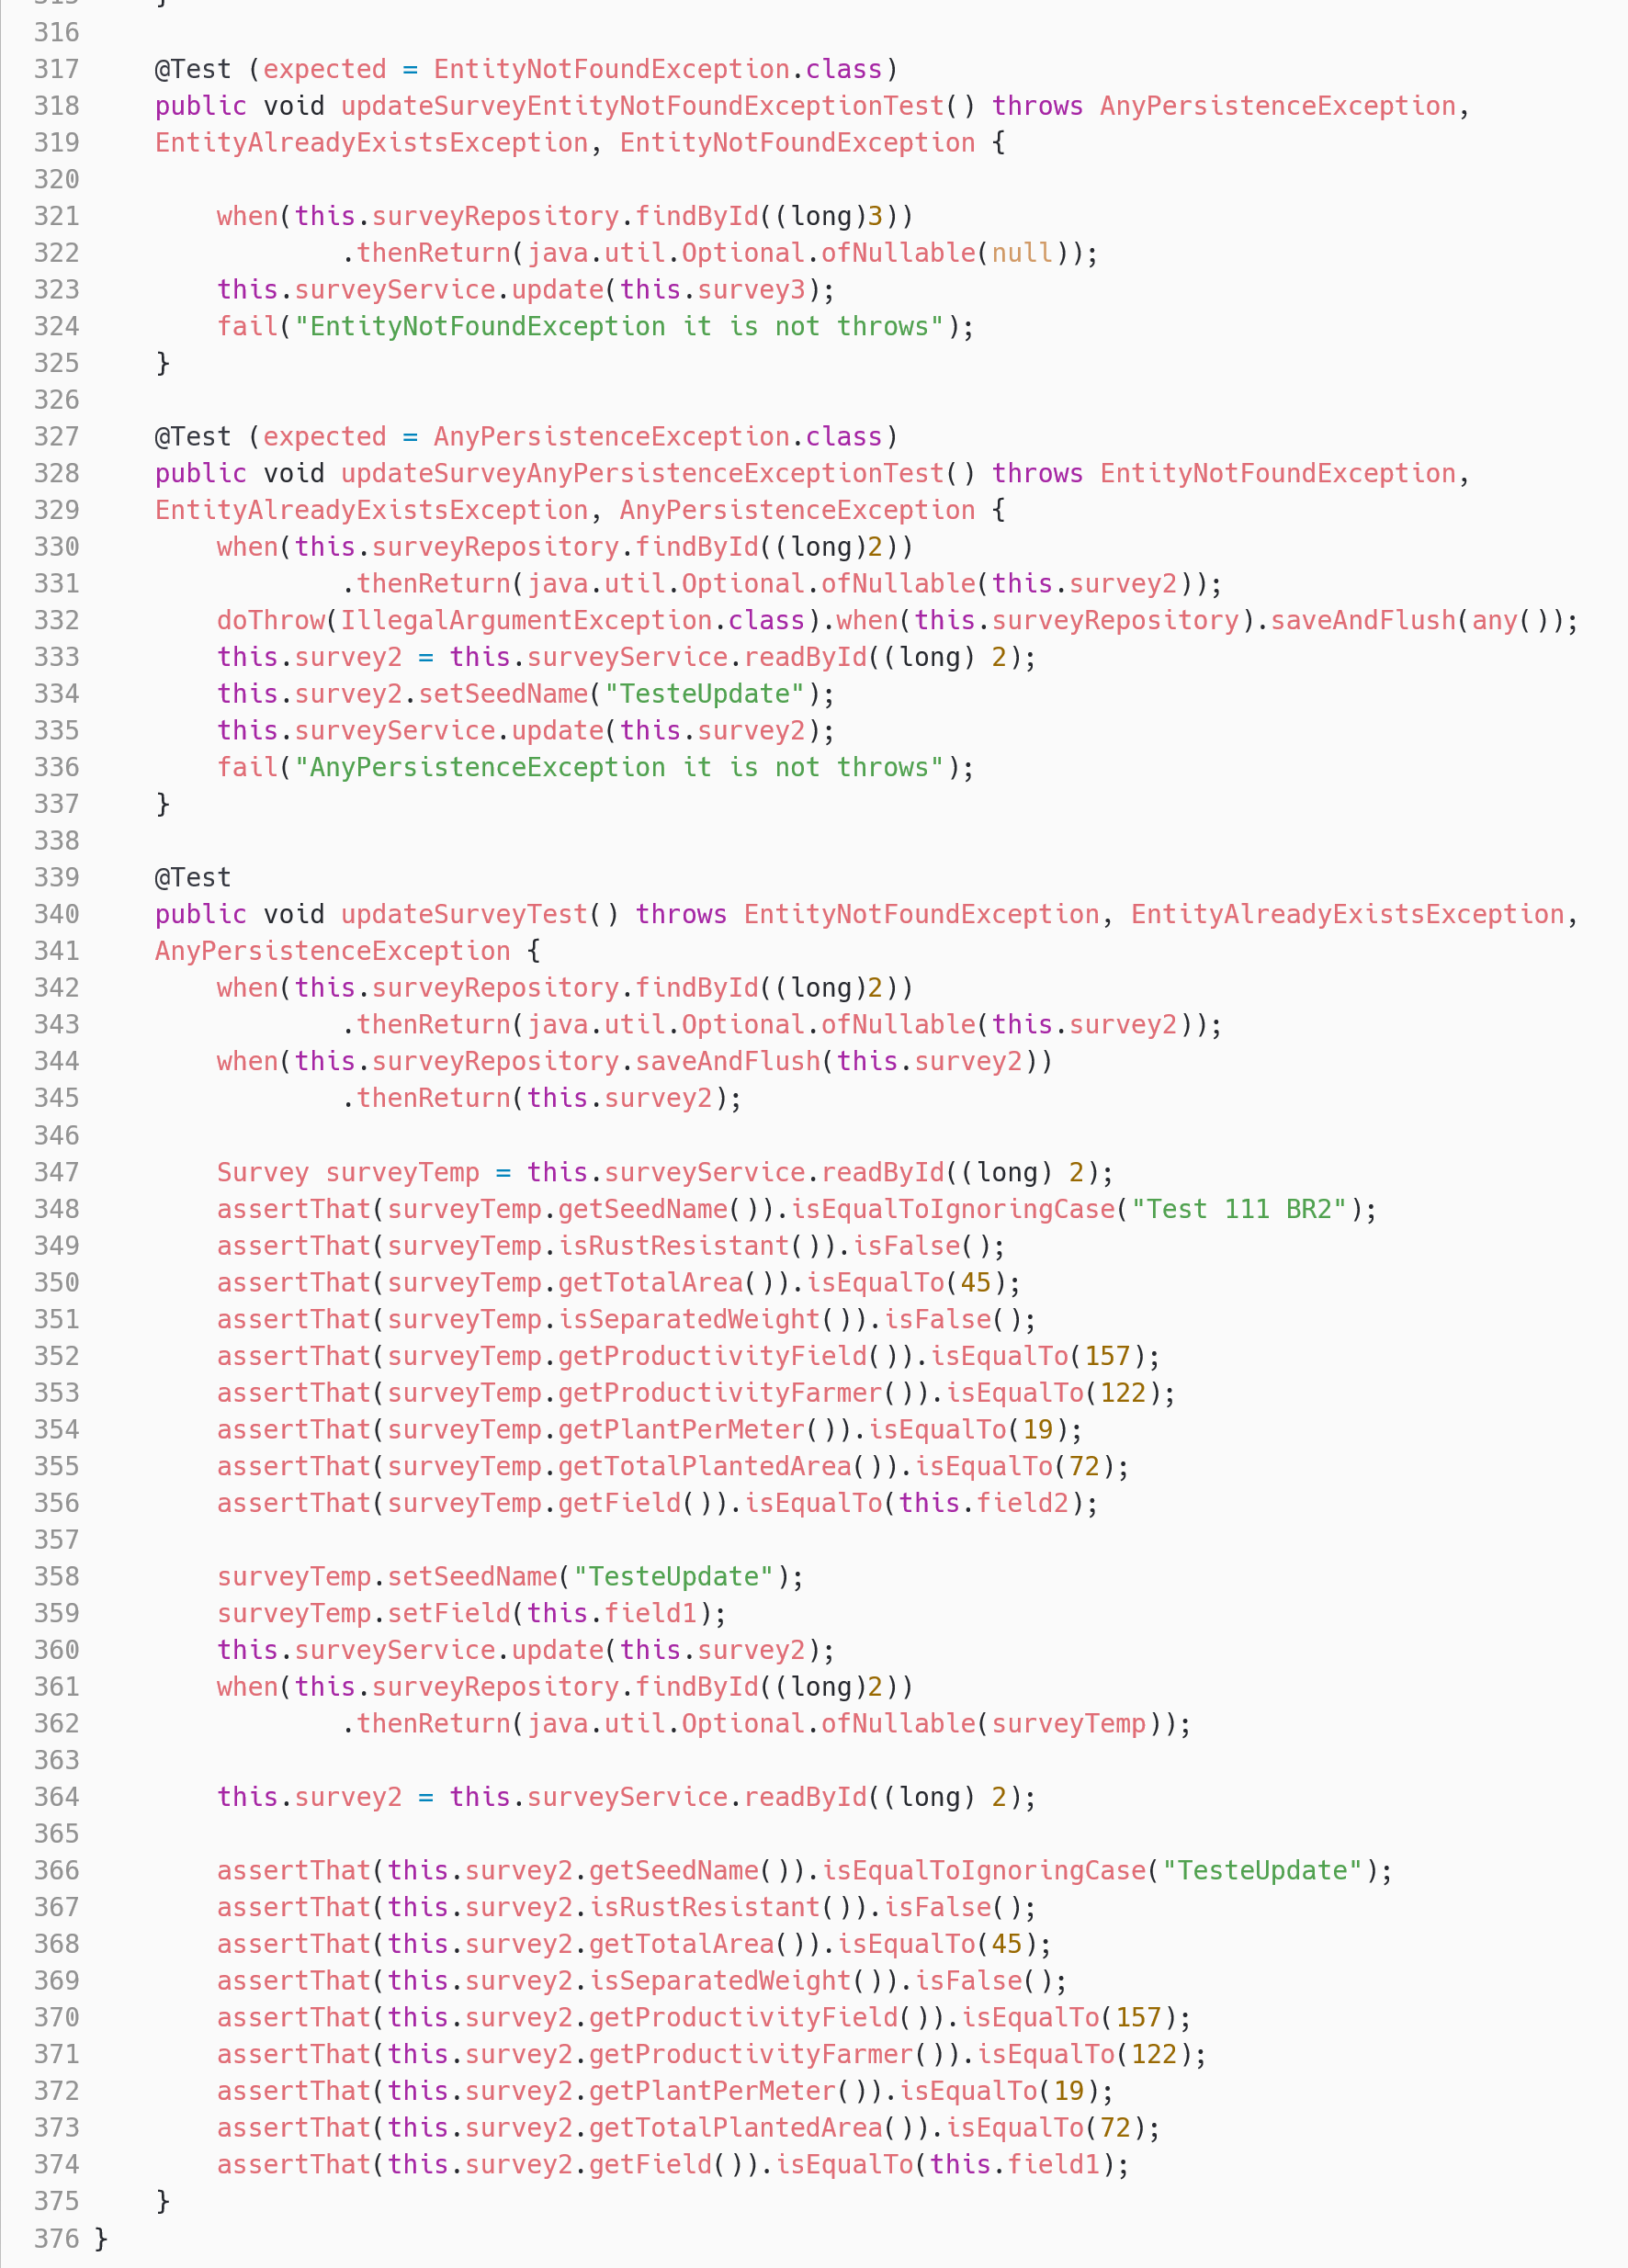
\includegraphics[scale=0.27]{dados/figuras/carbonSurveyService3.png}
	\caption{Classe de Teste  SurveyServiceTest.java.}
	\label{testeSurveyService}
\end{figure}

Método de teste \textit{ readByIdSurveyTest ()} linhas 117 a 123 figura \ref{testeSurveyService}: Este teste busca uma pesquisa na base de dados pelo seu identificador único. A entrada consiste em um numeral do tipo \textit{“Long”}. A saída é um objeto do tipo \textit{“Survey”}. Nesta assertiva o método testado deve retornar o registro \textit{mocado} nas linhas 119 e 120, o qual corresponde ao objeto comparado.

Método de teste \textit{ readByIdSurveyEntityNotFoundExceptionTest ()} linhas 125 a 131 figura \ref{testeSurveyService}: Este teste busca um registro do tipo \textit{“Survey”} na base de dados pelo seu identificador único, quando não encontrado é gerada uma exceção. A entrada consiste em um numeral do tipo \textit{“Long”}. A saída é uma exceção do tipo \textit{“EntityNotFoundException”}. Nesta assertiva o método testado deve retornar uma exceção, ao buscar um objeto pelo índice passado como parâmetro, ao realizar a consulta no banco um registro vazio é retornado, o que é simulado nas linhas 127 e 128, o que garante o lançamento da exceção \textit{“EntityNotFoundException”}.

Método de teste \textit{ readFieldbyIdTest ()} linhas 133 a 139 figura \ref{testeSurveyService}: Este teste busca um registro do tipo \textit{Field} na base de dados pelo seu identificador único. A entrada consiste em um numeral do tipo \textit{“Long”}. A saída é um objeto do tipo \textit{Field}. Nesta assertiva o método testado deve retornar o objeto \textit{mocado} nas linhas 135 e 136, o qual corresponde ao objeto comparado.

Método de teste \textit{ readFieldbyIdEntityNotFoundExceptionTest ()} linhas 141 a 147 figura \ref{testeSurveyService}: Este teste busca um registro do tipo \textit{Field} na base de dados pelo seu identificador único, quando não encontrado é gerada uma exceção. A entrada consiste em um numeral do tipo \textit{“Long”}. A saída é uma exceção do tipo \textit{“EntityNotFoundException”}. Nesta assertiva o método testado deve retornar uma exceção, ao buscar um objeto pelo índice passado como parâmetro, ao realizar a consulta no banco um registro vazio é retornado, o que é simulado nas linhas 143 e 144, o que garante o lançamento da exceção \textit{“EntityNotFoundException”}.

Método de teste \textit{ readHarvestByIdTest ()} linhas 150 a 157 figura \ref{testeSurveyService}: Este teste busca um registro do tipo \textit{“Harvest”} na base de dados pelo seu identificador único. A entrada consiste em um numeral do tipo \textit{“Long”}. A saída é um objeto do tipo \textit{“Harvest”}. Nesta assertiva o método testado deve retornar o objeto \textit{mocado} nas linhas 152 e 153, o qual corresponde ao objeto comparado.

Método de teste \textit{ readHarvestByIdEntityNotFoundExceptionTest ()} linhas 159 a 165 figura \ref{testeSurveyService}: Este teste busca um registro do tipo \textit{“Harvest”} na base de dados pelo seu identificador único, quando não encontrado é gerada uma exceção. A entrada consiste em um numeral do tipo \textit{“Long”}. A saída é uma exceção do tipo \textit{“EntityNotFoundException”}. Nesta assertiva o método testado deve retornar uma exceção, ao buscar um objeto pelo índice passado como parâmetro, ao realizar a consulta no banco um registro vazio é retornado, o que é simulado nas linhas 161 e 161, o que garante o lançamento da exceção \textit{“EntityNotFoundException”}.

Método de teste \textit{ readAllFieldsTest ()} linhas 167 a 175 figura \ref{testeSurveyService}: Este teste busca os registros do tipo \textit{Field} na base de dados. Não há entrada de dados.  A saída é uma lista do tipo \textit{Field}. Nesta assertiva o método testado deve retornar a lista criada na linha 169, que contém dois registros correspondentes a comparação.

Método de teste \textit{ readAllHarvestsTest ()} linhas 177 a 185 figura \ref{testeSurveyService}:  Este teste busca os registros do tipo \textit{“Harvest”} na base de dados. Não há entrada de dados.  A saída é uma lista do tipo \textit{“Harvest”}. Nesta assertiva o método testado deve retornar a lista criada na linha 179, que contém dois registros correspondentes a comparação.

Método de teste \textit{ readAllFieldsOutOfCurrentHarvestTest ()} linhas 187 a 195 figura \ref{testeSurveyService}: Este teste busca os registros do tipo \textit{Field} na base de dados que pertencem a colheita. A entrada é um numeral do tipo \textit{“Long”} identificador único de uma colheita.  A saída é uma lista do tipo \textit{Field} contendo os registros que pertencem a colheita. Nesta assertiva o método testado deve retornar a lista criada na linha 189, que contém um registro correspondente a comparação.

Método de teste \textit{ readByHarvestIdTest ()} linhas 197 a 201 figura \ref{testeSurveyService}: Este teste lista todas as pesquisas do banco de dados que contém uma determinada colheita. A entrada é um numeral do tipo \textit{“Long”} identificador único de uma colheita. A Saída é uma lista do tipo \textit{“Survey”} contendo as pesquisas salvas na base de dados que contem a colheita. Nesta assertiva o método testado deve retornar a lista criada na linha 106, que contem 2 objetos do tipo \textit{survey} correspondentes a comparação.

Método de teste \textit{ readByHarvestIdEntityNotFoundExceptionTest ()} linhas 205 a 209 figura \ref{testeSurveyService}: Este teste lança uma exceção do tipo \textit{“EntityNotFoundException”} quando não encontra uma pesquisa que contenha a colheita. A entrada é um numeral do tipo \textit{“Long”} identificador único de uma colheita. A Saída é uma exceção do tipo \textit{“EntityNotFoundException”}. Nesta assertiva o método testado deve lançar uma exceção do tipo \textit{“EntityNotFoundException”}.

Método de teste \textit{ deleteSurveyEntityNotFoundExceptionTest ()} linhas 211 a 218 figura \ref{testeSurveyService}: Este teste consiste em deletar um registro do tipo \textit{“Survey”}, mas o item a ser deletado não existe na base de dados. A Entrada consiste em um objeto do tipo \textit{“Survey”}. A Saída é o lançamento da exceção \textit{“EntityNotFoundException”}. A assertiva tenta deletar um registro, mas ao consultar o registro na base de dados simulada pelas linhas 214 e 215 o retorno é um nulo pois ele não existe na base, há o lançamento da exceção.  

Método de teste \textit{ deleteSurveyEntityInUseExceptionTest ()} linhas 220 a 228 figura \ref{testeSurveyService}: Este teste consiste em deletar um registro do tipo \textit{“Survey”}, mas o item a ser deletado está sendo utilizado na base de dados. A Entrada consiste em um objeto do tipo \textit{“Survey”}. A Saída é o lançamento da exceção \textit{“UseEntityInUseException”}. A assertiva tenta deletar um registro, mas este está sendo utilizado na base de dados simulada pela linha 225, há o lançamento da exceção.  

Método de teste \textit{ deleteSurveyAnyPersistenceExceptionTest ()} linhas 230 a 238 figura \ref{testeSurveyService}: Este teste consiste em deletar um registro do tipo \textit{“Survey”}, mas o item a ser deletado gera um erro na base de dados. A Entrada consiste em um objeto do tipo \textit{“Survey”}. A Saída é o lançamento da exceção \textit{“AnyPersistenceException”}. A assertiva tenta deletar um registro, mas um erro é gerado, há o lançamento da exceção.

Método de teste \textit{ deleteSurveyTest ()} linhas 240 a 255 figura \ref{testeSurveyService}: Este teste consiste em deletar um registro do tipo \textit{“Survey”}. A Entrada consiste em um objeto do tipo \textit{“Survey”}. Não há saída de dados.  A assertiva deleta um registro do banco linha 245, a validação é feita ao tentar consultar este registro no banco simulado e o retorno é uma exceção do tipo \textit{“EntityNotFoundException”}.  

Método de teste \textit{ createSurveyEntityNotFoundExceptionFieldTest ()} linhas 257 a 265 figura \ref{testeSurveyService}: Este teste consiste em criar um registro do tipo \textit{“Survey”}, mas o item a ser atualizado não possui um \textit{Field}. A Entrada consiste em um objeto do tipo \textit{“Survey”}. A Saída é o lançamento da exceção \textit{“EntityNotFoundException”}. A assertiva tenta criar um registro, mas ao buscar um registro do tipo \textit{Field} na base de dados simulada pela linha 261 o retorno é um nulo pois ele não existe na base, há o lançamento da exceção.  

Método de teste \textit{ createSurveyEntityAlreadyExistsExceptionTest ()} linhas 267 a 272 figura \ref{testeSurveyService}: Este teste consiste em tentar criar um novo registro do tipo \textit{“Survey”}, mas o item a ser criado é identificado como já existente na base de dados. A Entrada consiste em um objeto do tipo \textit{“Survey”}. A Saída é o lançamento da exceção \textit{“EntityAlreadyExistsException”}. A assertiva tenta inserir um registro que já se encontra na base de dados simulada pela linha 106, o que proporciona o lançamento da exceção.  

Método de teste \textit{ createSurveyEntityNotFoundExceptionHarversTest ()} linhas 274 a 284 figura \ref{testeSurveyService}: Este teste consiste em criar um registro do tipo \textit{“Survey”}, mas o item a ser atualizado não possui uma colheita. A Entrada consiste em um objeto do tipo \textit{“Survey”}. A Saída é o lançamento da exceção \textit{“EntityNotFoundException”}. A assertiva tenta atualizar um registro, mas ao buscar um registro do tipo \textit{“Harvest”} na base de dados simulada pela linha 280 o retorno é um nulo pois ele não existe na base, há o lançamento da exceção.  

Método de teste \textit{ createSurveyTest ()} linhas 286 a 302 figura \ref{testeSurveyService}: Este teste consiste em criar um novo registro do tipo \textit{“Survey”} na base de dados. A Entrada consiste em um objeto do tipo \textit{“Survey”}. O método não gera uma saída. A validação é feita através de um \textit{try cath}, que captura qualquer exceção que ocorra ao salvar o objeto. Como o método não lança uma exceção ele é aceito. A assertiva, no entanto, é feita através do repositório \textit{mocado} linhas 295 e 296, depois de inserido é simulada uma consulta pelo identificador único do objeto inserido o qual deve retornar o objeto que acaba de ser inserido.

Método de teste \textit{ createSurveyAnyPersistenceExceptionTest ()} linhas 304 a 315 figura \ref{testeSurveyService}: Este teste consiste em tentar criar um novo registro do tipo \textit{“Survey”}, mas o item a ser criado gera algum erro na base de dados. A Entrada consiste em um objeto do tipo \textit{“Survey”}. A Saída é o lançamento da exceção \textit{“AnyPersistenceException”}. A assertiva tenta inserir um registro na base de dados simulada pela linha 312, o que proporciona o lançamento da exceção.

Método de teste \textit{ updateSurveyEntityNotFoundExceptionTest ()} linhas 317 a 325 figura \ref{testeSurveyService}: Este teste consiste em atualizar um registro do tipo \textit{“Survey”}, mas o item a ser atualizado não existe na base de dados. A Entrada consiste em um objeto do tipo \textit{“Survey”}. A Saída é o lançamento da exceção \textit{“EntityNotFoundException”}. A assertiva tenta atualizar um registro, mas ao consultar o registro na base de dados simulada pela linha 321 o retorno é um nulo pois ele não existe na base, há o lançamento da exceção.  

Método de teste \textit{ updateSurveyAnyPersistenceExceptionTest ()} linhas 327 a 337 figura \ref{testeSurveyService}: Este teste consiste em atualizar um registro do tipo \textit{“Survey”}, mas o item a ser alterado gera um erro na base de dados. A Entrada consiste em um objeto do tipo \textit{“Survey”}. A Saída é o lançamento da exceção \textit{“AnyPersistenceException”}. A assertiva tenta atualizar um registro, mas ao alterar a base de dados simulada pela linha 332 o retorno é um exceção, há o lançamento da exceção.

Método de teste \textit{ updateSurveyTest ()} linhas 339 a 375 figura \ref{testeSurveyService}: Este teste consiste em atualizar um registro do tipo \textit{“Survey”}. A Entrada consiste em um objeto do tipo \textit{“Survey”}. Não há saída de dados. As assertivas consistem em recuperar um objeto da base de dados simulada linha 342, atualizar os campos deste objeto linhas 358 e 359, e em seguida atualizar esse registro na base linha 344. Caso não haja o lançamento de uma exceção o objeto atualizado é recuperado da base simulada, linha 361, e em seguida é feita as assertivas dos dados atualizados.

Após a execução dos testes a cobertura das entradas e saídas de dados da classe \textit{SurveyService}.java é de 100\%.



\subsection{RESULTADO GERAL DOS TESTES PACOTE SERVICE}

Para alcançar a cobertura de 100\% de todos os métodos linhas e classes do pacote Service foram criados no total 294 testes de unidade, onde 283 foram aprovados, 5 ignorados e 6 rejeitado. Cada classe possui o seguinte número de casos de teste: 

\begin{itemize}
        \item Pacote Base:
\begin{itemize}
    \item Classe \textit{FieldServiceTest}: 23 casos de teste aprovados;
    \item Classe \textit{RegionServiceTest}: 18 casos de teste aprovados, 1 reprovado;
    \item Classe \textit{FarmerServiceTest}: 12 casos de teste aprovados, 2 reprovados;
    \item Classe \textit{LocalDateTimeConverterTest}: 2 casos de teste aprovados;
    \item Classe \textit{MacroRegionServiceTest}: 12 casos de teste aprovados, 2 reprovados;
    \item Classe \textit{CityServiceTest}: 3 casos de teste aprovados;
    \item Classe \textit{SupervisorServiceTest}: 16 casos de teste aprovados, 1 reprovado;
\end{itemize}
  \item Pacote MIP:
  \begin{itemize} 
    \item Classe \textit{PestDiseaseServiceTest}: 14 casos de teste aprovados;
    \item Classe \textit{PestNaturalPredatorServiceTest}: 14 casos de teste aprovados; 
    \item Classe \textit{PestServiceTest}: 14 casos de teste aprovados;
    \item Classe \textit{MIPSampleServiceTest}: 18 casos de teste aprovados, 1 ignorado;
\end{itemize}
  \item Pacote \textit{Survey}:
  \begin{itemize}   
    \item Classe \textit{SurveyServiceTest}: 23 casos de teste aprovados, 1 ignorado;
    \item Classe \textit{HarvestServiceTest}: 14 casos de teste aprovados;
\end{itemize}
  \item Pacote MID:
  \begin{itemize}
    \item Classe \textit{BladeReadingResponsibleEntityServiceTest}: 18 casos de teste aprovados;
    \item Classe \textit{MIDRustSampleServiceTest}: 13 casos de teste aprovados;
    \item Classe \textit{BladeReadingResponsiblePersonServiceTest}: 18 casos de teste aprovados;
    \end{itemize}
    \item Pacote \textit{Pulverisation}:
  \begin{itemize}
    \item Classe \textit{ProductServiceTest}: 17 casos de teste aprovados, 1 ignorado;
    \item Classe \textit{PulverisationOperationServiceTest}: 20 casos de teste aprovados, 1 ignorado;
    \item Classe \textit{TargetServiceTest}: 14 casos de teste aprovados, 1 ignorado;
    \end{itemize}
    \end{itemize}



Como já dito anterior mente os testes podem garantir que o software é livre de defeitos mais, mas seu objetivo principal é revelar a presença de defeitos. Após a execução dos testes a taxa de cobertura foi de: 100\% das classes, 100\% dos métodos e 98\% das linhas. Como alguns casos de testes falharam não foi possível a cobertura de 100\% das linhas.


\section{TESTE IGNORADOS E REPROVADOS}

Em resumo, foram produzidos 652 testes de unidade, buscando a cobertura de 100\% das linhas, variáveis e métodos dos pacotes\textit{Entity}e Service do aplicativo MIP. Dentre eles 640 foram aprovados o equivalente a 98,16\% dos testes, 5 testes equivalente a 0,77\% foram ignorados e 7 falharam o que corresponde a 1,07\%.

\subsection{REPROVADOS}

Dos testes 7 casos falharam, os casos falhos e os motivos pelo qual falharam são listados a seguir:

  \begin{itemize}
    \item Pacote\textit{Entity}sub pacote \textit{base} classe \textit{Field}: O caso de teste \textit{“fieldTestAddSupervisorIsNull”} responsável por testar o método \textit{“field.addSupervisor(null)”} que recebe um nulo. O grande problema se deve na hora de fazer a listagem dos supervisores, ao percorrer a lista uma exceção do tipo \textit{“NullPointerException”} é lançada;

  \item Pacote \textit{Service} sub pacote \textit{base} classe \textit{FarmerServiceTest}: O caso de teste \textit{“updateFarmerServiceAnyPersistenceExceptionTest”}  responsável por testar o método \textit{“farmerService.update(Farmer)”} que atualiza um registro do tipo \textit{“Farmer”} deveria gerar uma exceção de persistência no banco de dados   ao tentar atualizar o registro, mas a exceção lançada é do tipo \textit{“EntityAlreadyExistsException”}. Antes da atualização o método de update recupera todos os registros do banco e verifica se o registro que será atualizado existe na lista, o que gera o lançamento da exceção pois o registro a ser atualizado não foi removido da lista;

  \item Pacote \textit{Service} sub pacote \textit{base} classe \textit{FarmerServiceTest}: O caso de teste \textit{“updateFarmerServiceTest”}  responsável por testar o método \textit{“farmerService.update(Farmer)”} que atualiza um registro do tipo \textit{“Farmer”} deveria atualizar o registro no banco de dados, mas é lançada uma exceção do tipo \textit{“EntityAlreadyExistsException”}. Antes da atualização o método de update recupera todos os registros do banco e verifica se o registro que será atualizado existe na lista, o que gera o lançamento da exceção pois o registro a ser atualizado não foi removido da lista;

  \item Pacote \textit{Service} sub pacote base classe \textit{MacroRegionServiceTest}: O caso de teste \textit{“updateMacroRegionServiceTest”  }responsável por testar o método \textit{“macroRegionService.update
  (macroRegion)”} que atualiza um registro do tipo \textit{“Macroregion” }deveria atualizar o registro no banco de dados, mas é lançada uma exceção do tipo \textit{“EntityAlreadyExistsException”}. Antes da atualização o método de update recupera todos os registros do banco e verifica se o registro que será atualizado existe na lista, o que gera o lançamento da exceção pois o registro a ser atualizado não foi removido da lista;

  \item Pacote \textit{Service} sub pacote base classe \textit{MacroRegionServiceTest: }O caso de teste \textit{“updateMacroRegionServiceAnyPersistenceExceptionTest”  }responsável por testar o método “macroRegionService.update(macroRegion)” que atualiza um registro do tipo\textit{ “Macroregion” }deveria gerar uma exceção de persistência no banco de dados   ao tentar atualizar o registro, mas a exceção lançada é do tipo \textit{“EntityAlreadyExistsException”}. Antes da atualização o método de update recupera todos os registros do banco e verifica se o registro que será atualizado existe na lista, o que gera o lançamento da exceção pois o registro a ser atualizado não foi removido da lista;

 \item Pacote \textit{Service} sub pacote \textit{base} classe \textit{RegionServiceTest}: O caso de teste\textit{ “readMacroRegionByIdRegionServiceEntityNotFoundExceptionTest”}  responsável por testar o método\textit{ “regionService.readMacroRegionById((long) 4)”} que busca um registro do tipo “MacroRegion” no banco de dados pelo identificador único gera uma exceção do tipo \textit{“NullPointerException”}. Quando o índice procurado não é encontrado há o lançamento de uma exceção do tipo \textit{“EntityNotFoundException”} a classe \textit{“RegionService”} faz o tratamento, retornando um objeto do tipo \textit{“MacroRegion”} vazio, mas ao utilizar o padrão \textit{Build} para a construção do objeto sem passar nenhum parâmetro o atributo nome que é do tipo \textit{string} é definido como \textit{null}, o que gera o lançamento da exceção na classe \textit{“MacroRegion” }no método \textit{“setName()”};

\item Pacote \textit{Service} sub pacote \textit{base} classe \textit{SupervisorServiceTest}: O caso de teste\textit{ “readRegionByIdSupervisorServiceEntityNotFoundExceptionTest”}  responsável por testar o método \textit{“supervisorService.readRegionById((long) 112)”} que busca um registro do tipo \textit{“Region” }no banco de dados pelo identificador único gera uma exceção do tipo\textit{ “NullPointerException”}. Quando o índice procurado não é encontrado há o lançamento de uma exceção do tipo \textit{“EntityNotFoundException”} a classe \textit{“SupervisorService” }faz o tratamento, retornando um objeto do tipo \textit{“Region” }vazio, mas ao utilizar o padrão \textit{Build} para a construção do objeto sem passar nenhum parâmetro o atributo nome que é do tipo \textit{string} é definido como \textit{null}, o que gera o lançamento da exceção na classe \textit{“Region”} no método \textit{“setName()”;}

    \end{itemize}



\subsection{IGNORADOS}

Foram ignorados 5 casos de testes, os casos ignorados e os motivos pelo qual foram ignorados são listados a seguir:
  \begin{itemize}
    \item Pacote \textit{Service} sub pacote mip classe \textit{MIPSampleServiceTest}: O teste \textit{“createSupervisorNotAllowedInCityTest}” foi ignorado pois o método testado “\textit{mipSampleService.create(new mipSampleTest)”} nuca lança a exceção \textit{“SupervisorNotAllowedInCity”};
    
\item Pacote \textit{Service} sub pacote survey classe SurveyServiceTest: O teste \textit{“readByHarvestIdEntityNotFoundExceptionTest”} foi ignorado pois o método testado \textit{“surveyService
.readByHarvestId(this.harvest3.getId())”} nuca lança a exceção \textit{“EntityNotFoundException”} mas retorna uma lista vazia;

\item Pacote \textit{Service} sub pacote \textit{pulverisation} classe \textit{PulverisationOperationServiceTest}: O teste “createPulverisationOperationServiceEntityNotFoundExceptionTest” foi ignorado pois o método testado “pulverisationOperationService.create(new pulverisationOperation)” nuca lança a exceção \textit{“EntityNotFoundException”};

\item Pacote \textit{Service} sub pacote \textit{pulverisation} classe \textit{ProductServiceTest}: O teste\textit{ “createProductServiceEntityNotFoundExceptionTest”} foi ignorado pois o método testado\textit{ “productService.create(new product)”} nuca lança a exceção \textit{“EntityNotFoundException”};

\item Pacote \textit{Service} sub pacote \textit{pulverisation} classe \textit{TargetServiceTest}: O teste “\textit{createTargetServiceEntityNotFoundExceptionTest}” foi ignorado pois o método testado “\textit{targetService.create(new target3)}” nuca lança a exceção \textit{“EntityNotFoundException”};


    \end{itemize}
                    % Resultados
% % \chapter{CONSIDERAÇÕES FINAIS}



% O teste de software é um processo custoso e que demanda muitos recursos e tempo para ser planejado e executado, porém é parte fundamental no desenvolvimento de sistemas que buscam por qualidade.  O principal objetivo do presente trabalho é cobrir totalmente os testes de unidade e testes de componentes do sistema MIP, buscando a verificação e validação dos requisitos coletados promovendo uma melhoria do sistema como um todo. Estas etapas são apenas o início de um plano de teste de software. Ainda restam outras etapas que devem ser implementadas como o teste de sistema e teste de aceitação que não serão tratados neste trabalho e devem ser explorados em trabalhos futuros. 

\chapter{DESENVOLVIMENTO}

Este capítulo apresenta as configurações iniciais que foram necessárias para a execução dos testes de unidades no aplicativo MIP. 

\section{CONFIGURAÇÕES INICIAIS}

\subsection{Estrutura do Projeto}



A estrutura de diretórios gerados pelo \textit{framework Spring Boot} garante a divisão do código fonte, promovendo a separação das classes e suas responsabilidades. Além disso é possível adotar uma subestrutura, está deve seguir um padrão arquitetural mantendo a organização e facilitando a manutenção do projeto. A FIGURA \ref{estruturaProjeto} apresenta o estado atual do projeto e suas divisões em diretórios e subdiretório. 


\begin{figure}[H]
	\centering
	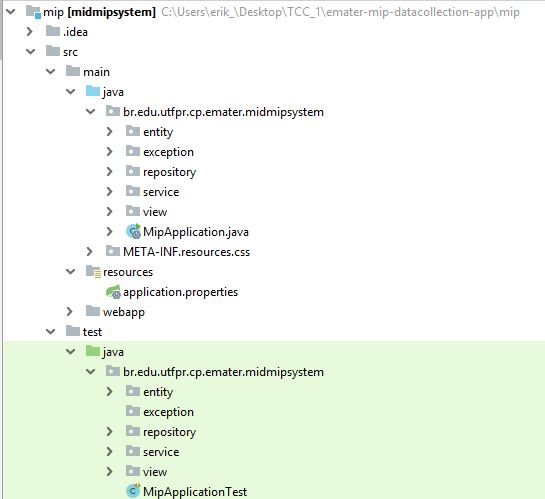
\includegraphics[]{dados/figuras/estruturaDoProjeto.JPG}
	\caption{Estrutura do projeto \textit{Spring Boot.}}
	\label{estruturaProjeto}
\end{figure}

    Um diretório pode conter nenhum, um ou mais de um subdiretório ou classes dentro dele. O projeto apresentado na FIGURA \ref{estruturaProjeto}  segue o padrão de nomenclatura especificado  pela convenção de código Java publicado pela \textit{Sun} e mantida pela \textit{Oracle} \cite{Oracle}, juntamente de diretórios pré-configurados pelo \textit{Spring-Boot} e pelo \textit{Maven} o que permite a familiarização imediata de novos usuários que já utilizaram o \textit{framework.} Estes diretórios possuem o seguinte contexto: 



\begin{itemize}
    \item \textbf{src/main/java:} Diretório onde está o código fonte Java da Aplicação.
\item \textbf{src/main/META-INF.resources.css:} Diretório usado para configurar informações de metadados do projeto, geralmente dados web como folhas de estilo CSS.
\item \textbf{src/main/resources:} Arquivos de configuração e outros arquivos devem ficar nesta pasta.
\item \textbf{src/main/webapp:} Diretório para conteúdo Web. Aqui se encontra todos os arquivos fonte da parte web.
\item \textbf{src/test/java:} Diretório que contém os arquivos de testes unitários.
\item \textbf{src/test/resources:} Diretório com arquivos que serão utilizados pelas classes de testes unitários
\end{itemize}


O padrão da \textit{Sun} utilizado para dar nome aos subdiretórios é relativo ao nome da instituição em que o projeto é desenvolvido:

\begin{itemize}
 
\item \textbf{br/edu/utfpr/cp/emater/midmipsystem/}
\end{itemize}


Os diretório só possuem letras minúsculas, não importa quantas palavras estejam contidas nele. Esse padrão existe para evitar ao máximo o conflito de diretório de instituições diferentes.

Os subdiretórios representam a divisão arquitetural em camadas do sistema onde cada diretório possui a seguinte responsabilidade: 

\begin{itemize}
 

\item \textbf{Entity (Domínio):} Implementa entidades, interfaces para serviços, validações e classes do domínio. 


\item \textbf{Repository (Infraestrutura):} Implementa a persistência dos dados e os repositórios.

\item \textbf{Service (Serviços):} Implementa a comunicação da aplicação com a interface.

\item \textbf{View (Apresentação):} Implementa a interface do usuário.

\item \textbf{Exception:} Implementa o tratamento de erros específicos que podem acontecer durante execução da aplicação.
\end{itemize}

O diretório de \textit{test} segue o modelo estrutural do diretório main e seus subdiretórios, mais por convenção toda classe do diretório de teste deve seguir o padrão: classe+Test. O que proporciona a identificação e a separação das classes de testes.  

\subsection{Controle de versão}

Para realizar o controle de versão do projeto será utilizado o \textit{Git} na máquina local e o \textit{Github} como repositório remoto. O \textit{Github} possibilita que uma equipe de desenvolvimento trabalhe de forma centralizada e organizada auxiliando a manter o histórico de alterações do projeto permitindo ao administrador controlar o que é alterado, quando foi alterado e qual usuário alterou, possibilitando a voltar a uma versão mais estável caso uma alteração gere uma inconsistência.

 Por se tratar de um trabalho colaborativo o repositório do projeto já estava criado no endereço: \textit{https://github.com/gabrielcostasilva/emater-mip-datacollection-app}, porem para que as alterações não fossem realizadas diretamente no projeto original podendo gerar erros, foi feito um clone da versão original gerando um novo repositório no endereço: \textit{https://github.com/ErikZA/emater-mip-datacollection-app}. Posteriormente as alterações feitas no projeto clonado podem ser enviadas ao repositório original através de um \textit{pull request}\footnote{Pull Request é quando se envia uma sugestão de melhoria para o repositório.}. O administrador avaliará as alterações, depois da análise de impacto ele deve aceitá-las ou recusá-las.




\subsection{Controle do projeto}

O \textit{Github} também oferece diversas ferramentas para melhorar o controle do projeto. Depois de criar ou clonar um repositório é possível adicionar tarefas que devem ser resolvidas chamadas de \textit{"issues”} pelo \textit{Github}. Estas \textit{issues} podem receber diferentes etiquetas de acordo com o impacto que elas têm no projeto. A FIGURA \ref{issues} apresenta as \textit{issues} que foram criadas para este projeto assim como a etiqueta que cada uma delas recebeu de acordo com o seu impacto:

\begin{figure}[H]
	\centering
	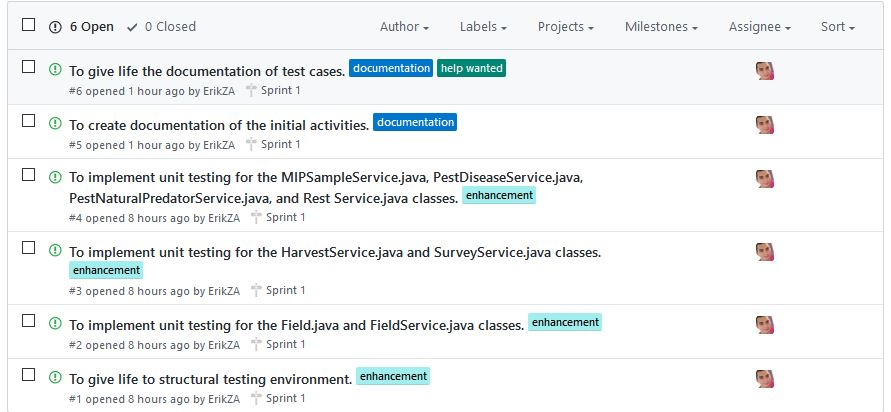
\includegraphics[scale=0.7]{dados/figuras/issues.JPG}
	\caption{\textit{Issues} do projeto.}
	\label{issues}
\end{figure}


As \textit{issues} listadas na FIGURA \ref{issues} tem as seguintes funções:


\begin{itemize}
 \item[1] \textit{To give life to structural testing environment. Label: enhancement (New feature or request)}\footnote{Para dar vida ao ambiente de testes estruturais. Etiqueta: valorização (novo recurso ou pedido)}

\item \textit{It consists of adding the necessary dependencies and creating the structure of folders that allow the execution of the unit tests.}\footnote{Consiste em adicionar as dependências necessárias e criar a estrutura das pastas que permitem a execução dos testes unitários.}

 \item[2] \textit{To implement unit testing for the Field.java and FieldService.java classes. Label: enhancement (new feature or request)}\footnote{Para implementar testes de unidade para as classes Field.java e FieldService.java. Etiqueta: valorização (novo recurso ou pedido)}

\item \textit{Consist on testing the Field.java and FieldService.java classes.}\footnote{Consistem em testar as classes Field.java e FieldService.java.}

 \item[3] \textit{To implement unit testing for the HarvestService.java and SurveyService.java classes. Label: enhancement (new feature or request)}\footnote{Para implementar testes de unidade para as classes HarvestService.java e SurveyService.java. Etiqueta: valorização (novo recurso ou pedido)}

\item \textit{Consist on testing the HarvestService.java and SurveyService.java classes.}\footnote{Consistem em testar as classes HarvestService.java e SurveyService.java.}

 \item[4] \textit{To implement unit testing for the MIPSampleService.java, PestDiseaseService.java, PestNaturalPredatorService.java, and Rest Service.java classes. Label: enhancement (new feature or request)}\footnote{Para implementar testes de unidade para as classes MIPSampleService.java, PestDiseaseService.java, PestNaturalPredatorService.java e Rest Service.java. Etiqueta: valorização (novo recurso ou pedido)}

\item \textit{Consist of testing the MIPSampleService.java, PestDiseaseService.java, PestNaturalPredatorService.java, and PestService.java.}\footnote{Consiste em testar o MIPSampleService.java, o PestDiseaseService.java, o PestNaturalPredatorService.java e o PestService.java.}


 \item[5] \textit{To create documentation of the initial activities. Label: Documentation (Improvements or additions to documentation)}\footnote{
Para criar documentação das atividades iniciais. Etiqueta: documentação (melhorias ou adições a documentação)}

\item \textit{Preparation of the tcc2 document.}\footnote{Elaboração do documento tcc2.}

 \item[6] \textit{To give life the documentation of test cases. Documentation (Improvements or additions to documentation), label: help wanted (Extra caution is required)}\footnote{Para dar vida a documentação dos casos de teste. Etiqueta: documentação (melhorias ou adições a documentação), etiqueta: Procura-se ajuda (é necessária cautela Extra)}
 
\item \textit{Create documentation of the initial activities. Flow Graph Notation. Cyclomatic Complexity. Derivation of Test Cases.}\footnote{Notação de Fluxograma. Complexidade ciclomática. Derivação de Casos de Teste.}

\end{itemize}{}




Além disso e possível marcar uma data no projeto chamado no Github de “Milestones”, esta marcação foi utilizada de forma a estipular uma data de conclusão de um determinado conjunto de issues do projeto, é possível associar está marcação as issues facilitando o controle e o monitoramento do projeto. A FIGURA \ref{splint1} apresenta os milestones criados para o projeto: 
\begin{figure}[H]
	\centering
	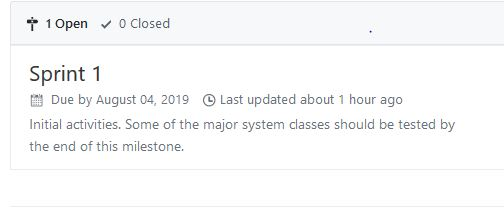
\includegraphics[scale=1.1]{dados/figuras/milestones.JPG}
	\caption{Marco para o primeiro Sprint.}
	\label{splint1}
\end{figure}

Cada milestones representa a entrega de um conjunto de funcionalidades do projeto, cada entrega foi definida da seguinte forma:

\begin{itemize}
    \item[1]\textit{\textbf{Sprint 1} Initial activities. Some of the major system classes should be tested by the end of this milestone.}\footnote{Atividades iniciais. Algumas das principais classes do sistema devem ser testadas até o final desse marco.}
    \item \textit{Due by August 04, 2019}\footnote{ Entrega até 04 de agosto de 2019}
\end{itemize}{}

Após criar as \textit{issues} e os \textit{milestone} é possível associá-los a um \textit{Github projects}, que permite criar fases de execução do projeto. Esta ferramenta permite controlar a execução das issues atribuindo-as a uma fase dentro do projeto.  A FIGURA \ref{controleAtividades} apresenta o controle da execução das \textit{issues} e as fases do projeto:

A FIGURA \ref{controleAtividades} apresenta o projeto, suas fases e a posição de cada \textit{issues} dentro do projeto.   O projeto possui 4 fases: \textit{To do} (Façam); \textit{In progress} (Em progresso); \textit{In revision} (Em revisão); \textit{Done} (Feito). Uma nova \textit{issue} deve entrar no projeto na fase \textit{To do}, esta fase indica que a tarefa ainda deve ser realizada. Quando a issue seguir para produção ela deve passar para a fase \textit{in progress}, o que indica que a atividade esta sendo realizada. Posteriormente esta atividade deve ser apresentada e revisada ao final de cada \textit{milestones}, está fase é a \textit{In revision}. Após a apresentação e validação das atividades executadas a atividade é direcionada a fase \textit{Done}, o que encerra a \textit{issue}.
\begin{landscape}
\begin{figure}[H]
	\centering
	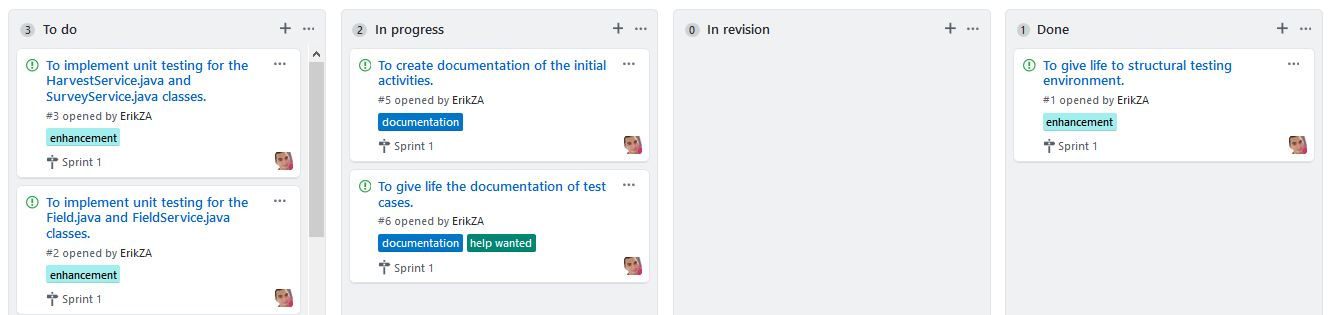
\includegraphics[scale=0.7]{dados/figuras/atividadesProjeto.JPG}
	\caption{Controle das atividade.}
	\label{controleAtividades}
\end{figure}
\end{landscape}



\section{LIÇÕES APRENDIDAS}

\begin{itemize}
    \item Uma das diferenças da faculdade para um projeto de trabalho real é que o curso superior te prepara para uma área de conhecimento, o que dá ao aluno um conhecimento muito mais teórico. Enquanto projetos de trabalho exigem uma formação muito mais técnica e um profundo conhecimento de ferramentas e frameworks que oferecem um conjunto de funcionalidades prontas, o que torna a teoria pouco eficiente nestes casos pois o projeto exige produtividade.
    
    \item A defasagem de muitos cursos é um problema, a universidade tenta construir uma base solida de conhecimento para cada aluno, mas muitos cursos estão desatualizados ou acabam não atingindo o objetivo por falta de carga horaria ou ementa desatualizada. O fato é que a tecnologia se atualiza muito rápido é muito do que é ensinado ainda é muito básico para o mercado que em sua maioria exige profissionais que conheçam as mais novas tecnologias. Talvez a burocracia publica atrapalhe a UTFPR neste ponto.
    
    \item O mercado de trabalho está muito exigente o que torna um profissional graduado pouco relevante, a falta de certificações técnicas oficias faz falta na formação pois certificações JAVA ou outras ajudariam no desenvolvimento de projetos e na formação do profissional.
    
\end{itemize}{}



% \chapter{EQUAÇÕES}

% \chapter{SOBRE AS LISTAS}

% \chapter{SOBRE AS CITAÇÕES E CHAMADAS DE REFERÊNCAS}



   


\chapter{RESULTADOS}

Este capitulo expõe os resultados obtidos através da execução dos testes de unidade no aplicativo MIP, como o número de testes desenvolvidos durante o desenvolvimento do trabalho é extenso foram escolhidas as principais classes do pacote \textit{Entity} (\textit{Field.java e Survey.java}), e as principais classes do pacote \textit{Service} (\textit{FieldService.java e SurveyService.java}). para serem analisadas profundamente. 


\section{APURAÇÃO DOS TESTES PACOTE ENTITY}

O pacote \textit{Entity} é responsável por armazenar as classes que realizam o mapeamento objeto-relacional, e nele é definida as principais regras de negócio do sistema. O pacote é composto por 5 sub pacotes sendo eles: 

\begin{itemize}

\item[1]Pacote \textit{base}: Armazenas as classes que define a estrutura básica do sistema, as classes que definem regiões (\textit{Region.java}), cidades (\textit{City.java}), estados (\textit{State.java}) e macrorregiões (\textit{MacroRegion.java}), assim como as que definem supervisores (\textit{Supervisor.java}) e agricultor (\textit{Farmer.java}). Todos esses dados compõem um registro (\textit{Field.java}) que estabelece uma ligação entre localização, supervisores e agricultor. Além disso o pacote contém mais duas superclasses, \textit{AuditingPersistenceEntity.java} responsável por armazenar metadados dos objetos, e \textit{Person.java} responsável por definir os atributos básicos de uma pessoa.  

\item[2]Pacote mid: Armazena as classes que definem a estrutura básica para coleta e análise de esporos de ferrugem asiática e doenças que afetam a lavoura. A classe \textit{AsiaticRustTypesLeafInspection.java} contém os tipos de lesões causadas pela ferrugem em plantas, a classe \textit{AsiaticRustTypesSporeCollector.java} contém os tipos de análise que podem ser retiradas do coletor de esporos, a classe \textit{BladeReadingResponsibleEntity.java} armazena a entidade responsável pela leitura de laminas de esporos, classe \textit{BladeReadingResponsiblePerson.java} é responsável por armazenar a pessoa responsável pela leitura de esporos, \textit{MIDSampleSporeCollectorOccurrence.java} trata os dados da amostra de esporos coletada, \textit{MIDSampleLeafInspectionOccurrence.java} trata os dados da inspeção das folhas coletada, \textit{MIDSampleFungicideApplicationOccurrence.java} trata os dados da aplicação de fungicida contra a ferrugem. A classe principal deste pacote é a \textit{MIDRustSample.java} pois é nela onde são armazenados todos os registros de aplicação de fungicida, de coleta de folhas, de coleta de sopros e os responsáveis pelas análises. 

\item[3]Pacote mip: Armazena as classes que definem a estrutura básica para coleta e análise de pragas que atingem a lavoura.  A classe \textit{Pest.java} registra os tipos de pragas que podem atingir uma lavoura, \textit{PestDisease.java} armazena as doenças causadas por pragas, \textit{PestSize.java} é responsável pelo armazenamento do tamanho das pragas. \textit{GrowthPhase.java} registra a fase de crescimento em que a praga foi encontrada, \textit{PestNaturalPredator.java} armazena os predadores naturais das pragas, \textit{MIPSamplePestOccurrence.java} registra a ocorrência de pragas em uma lavoura, \textit{MIPSamplePestDiseaseOccurrence.java} registra a ocorrência de doenças causadas por pragas em uma lavoura, \textit{MIPSampleNaturalPredatorOccurrence.java} registra a ocorrência de predadores naturais na lavoura. A classe principal deste pacote é a \textit{MIPSample.java} ela é responsável por armazenar os dados de pragas, doenças causadas por pragas e predadores naturais que atingem uma lavoura.

\item[4]Pacote \textit{pulverisation}: Armazena as classes que definem a estrutura básica para a atividade de pulverização de uma lavoura. As classes \textit{ProductUnit.java} e \textit{Product.java} são responsáveis por tratar dos produtos que serão utilizados durante a pulverização, definem unidade de medida do produto e características do produto como nome e dose respectivamente. As classes \textit{TargetCategory.java} e \textit{Target.java} definem a categoria alvo do pesticida e qual praga ele combate respectivamente. A classe \textit{PulverisationOperationOccurrence.java} define uma ocorrência de pulverização.  A principal classe deste pacote é a \textit{PulverisationOperation.java} esta contém os dados referente a todas as pulverizações que foram realizadas. 

\item[5]Pacote \textit{survey}: Armazena as classes que definem a estrutura básica para realizar uma pesquisa de campo através dos dados coletados com o manejo integrado de pragas e com o manejo integrado de doenças. A classe \textit{DateData.java} armazena os dados de uma colheita como data de semeadura e data da colheita, a classe \textit{SizeData.java} contém os dados referente a área da colheita, a classe \textit{LocationData.java} contém dados referente a localização da colheita, a classe \textit{ProductivityData.java} contém dados referente a produtividade de uma colheita, a classe \textit{QuestionData.java} registra dados específicos referente a plantação, se a plantação é resistente a ferrugem por exemplo, a classe \textit{Harvest.java} e responsável por registrar dados referente a colheita como o início e o fim da colheita. A principal classe deste pacote é a \textit{Survey.java} ela é responsável por armazenar todos os dados referente a uma pesquisa da produção da lavoura de um produtor.

\end{itemize}{}

\subsection{RESULTADO DOS TESTES CLASSE FIELD.JAVA}

Como já foi ressaltado anteriormente uma das principais classes do sistema é a \textit{Field.java}, a FIGURA \ref{diagrmaTestField} apresenta o diagrama de classes que expressa a classe \textit{Field.java}, e as demais classes que a compõem assim como a classe responsável por testá-la, a classe FieldTest.java. Também é possível analisar no diagrama os atributos e métodos que pertence à classe \textit{Field}, assim como os métodos e atributos da classe de teste \textit{FieldTest}.

\begin{figure}[H]
	\centering
	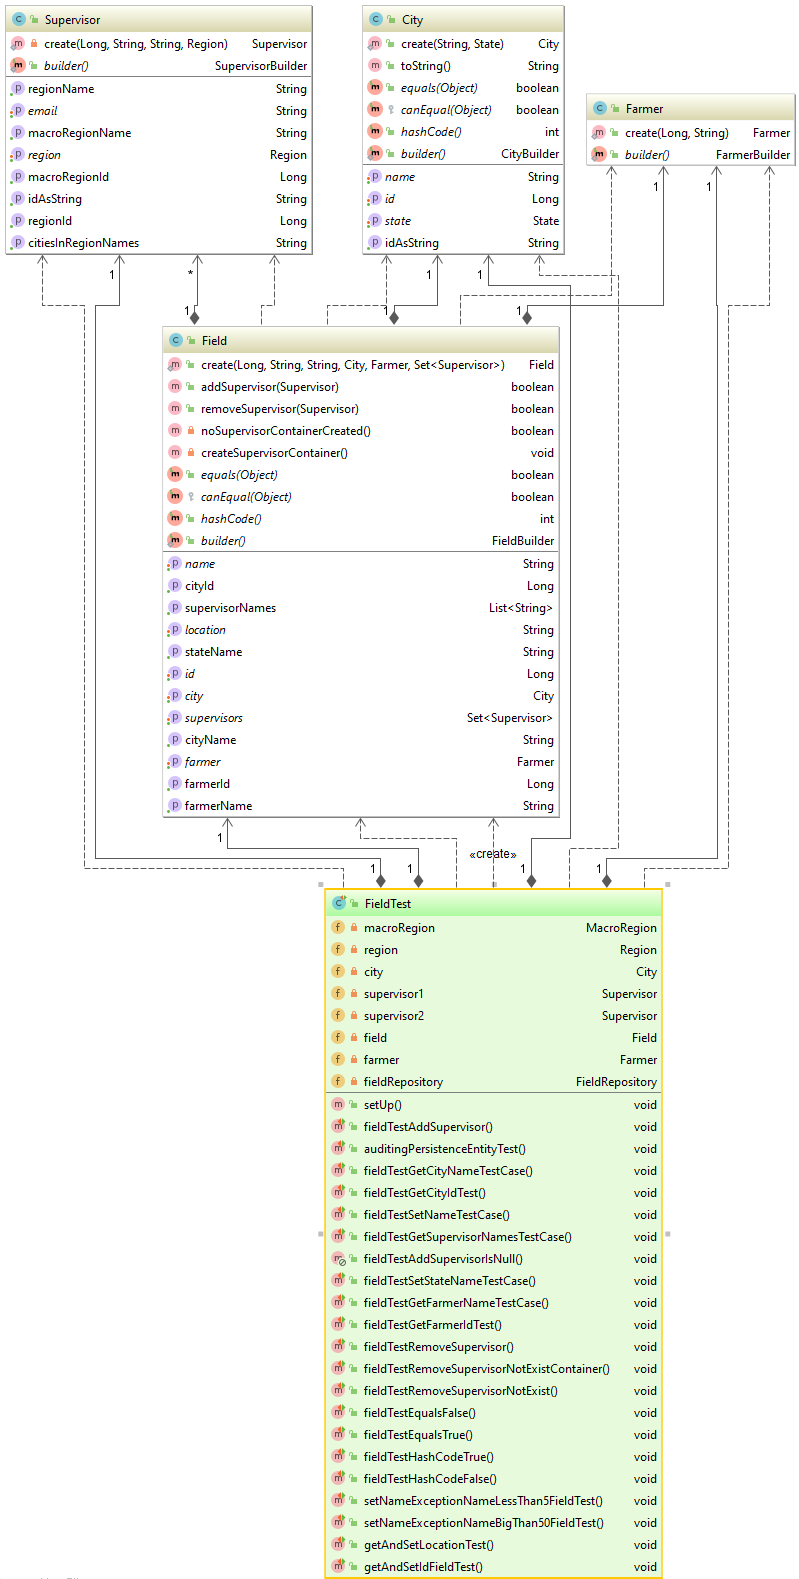
\includegraphics[scale=0.58]{dados/figuras/PackagebaseTestField.png}
	\caption{Diagram de Classes Field e FieldTest.}
	\label{diagrmaTestField}
\end{figure}

A classe de teste apresentada na FIGURA \ref{diagrmaTestField} possui vinte e um métodos de teste e um método de apoio aos testes denominado \textit{“setUp”}, o objetivo dos testes é exercitar a classe \textit{Field} até que todos as variáveis, entradas e saídas de dados sejam executados pelo menos uma vez. Como a classe \textit{Field} é composta por outras classes se faz necessário a instanciação de outras classes como \textit{Supervisor}, \textit{Farmer}, \textit{City} e outras para a execução completa dos testes. Como a classe se trata de uma entidade que será persistida em um banco de dados, ela possui certas regras de negócio que serão ativadas somente no momento de gravar os dados no banco, sendo assim foi preciso criar uma referência para a interface \textit{FieldRepository}, classe responsável por realizar a persistência dos dados no banco. Como o objetivo deste trabalho é cobrir o sistema com testes unitários e testes que integram classes entidades com o banco de dados ou comunicação com \textit{APIs} são testes de integração foi utilizado um\textit{ “Mock”} para simular o comportamento do repositório.

A FIGURA \ref{field1} apresenta a declaração da classe de testes, os atributos utilizados para desenvolver os testes e o método\textit{ “setUp”} utilizado para preparar o ambiente para os testes.


O trecho de código da FIGURA \ref{field1} apresenta as seguintes funcionalidades:





\begin{itemize}

\item Na linha 1 é utilizada a anotação \textit{@SpringBootTest} que prepara um contexto \textit{Spring} e inclui a possibilidade de iniciar um container em um porta default ou configurada pelo usuário. O que não é necessário para o tipo de teste executado nesta classe; 

 \item Na linha 2 é utilizada a anotação \textit{@FixMethodOrder} que permite definir uma ordem de execução dos testes, neste casso foi definida a ordem \textit{“NAME\_ASCENDING"} que faz a execução dos testes de acordo com o nome de maneira ascendente;

 \item Linha 3 a classe \textit{FieldTest} é aberta;

 \item Da linha 5 a 10 há a declaração dos objetos que serão utilizadas nos testes;
 
  \item Na linha 12 um objeto do tipo \textit{FieldRepositorio} e declarado e instanciado como um objeto \textit{mock}.

 \item Na linha 15 é utilizado a anotação \textit{@Before}, esta anotação determina que, sempre antes da execução de um teste o método \textit{“setUp”} deve ser executado primeiro.

 \item O método \textit{“setUp”} que tem sua declaração na linha 15 e vai até a linha 30 é responsável por realizar a construção dos objetos declarados nas linhas 5 a 10.


\end{itemize}{}



A FIGURA \ref{field1} apresenta os casos de testes criados para a classe \textit{Field}. 


A ideia geral na elaboração dos testes é a de cobrir cada atribuição de dados, as entrada e saída de dados da classe \textit{Field}, buscando a cobertura de 100\% das linhas métodos e atributo da classe. Os resultados obtidos da execução dos testes foram listados a seguir:

Método de teste \textit{“fieldTestAddSupervisor()”} linhas 32 a 36 figura \ref{field1}: Este método é responsável por testar se um objeto do tipo\textit{ “supervisor”} é adicionado ao objeto testado através do método de entrada \textit{“field.addSupervisor(Supervisor supervisor)”}.  Neste teste a entrada é um objeto do tipo \textit{“Supervisor” }e a saída do método é uma variável do tipo \textit{“boolean”}(verdadeiro ou falso).  As entradas foram criadas nas linhas 24 e 26 e fornecidas como entradas ao método testado nas linhas 34 e 35 respectivamente. A saída é um \textit{“TRUE”} já que os objetos passados são adicionados a classe\textit{ “Field”}. 



Método de teste\textit{ “auditingPersistenceEntityTest()”} linhas 38 a 47 figura \ref{field1}: Este método é responsável por testar os atributos criados na superclasse\textit{ “auditingPersistenceEntity”}, como uma superclasse não pode ser testada os métodos e atributos dela devem ser testados em uma das subclasses.  A classe é composta por dois atributos do tipo \textit{long “LastModified”} e \textit{“CreatedAt”,} O objetivo deste teste é de atribuir valor as variáveis e verificar se os valores atribuídos são recuperados corretamente. As entradas foram criadas nas linhas 40 e 41 e atribuídas ao objeto testado nas linhas 43 e 44 respectivamente. Posteriormente nas linhas 45 e 46 é feita a confirmação das saídas contendo os valores 11 e 12 do tipo \textit{“long”.}

Método de teste \textit{“fieldTestGetCityNameTestCase ()”} linhas 49 a 52 figura \ref{field1}: Este caso de teste verifica se um nome atribuído a uma cidade é recuperado pelo método \textit{“field.getCityName()”.} A entrada é uma \textit{String} de caracteres, e a saída deve ser uma \textit{String} de caracteres formatados com a primeira letra de cada palavra maiúscula.  O objeto do tipo \textit{“city” }é criado na linha 19 o atribuído nome é definido como “NOvA FAtimA” em seguida o objeto\textit{ “city”} é atribuído ao objeto\textit{ “Field” }na linha 28 /29. Já no teste o valor e recuperado é o retorno é “Nova Fatima”.


\begin{figure}[H]
	\centering  
	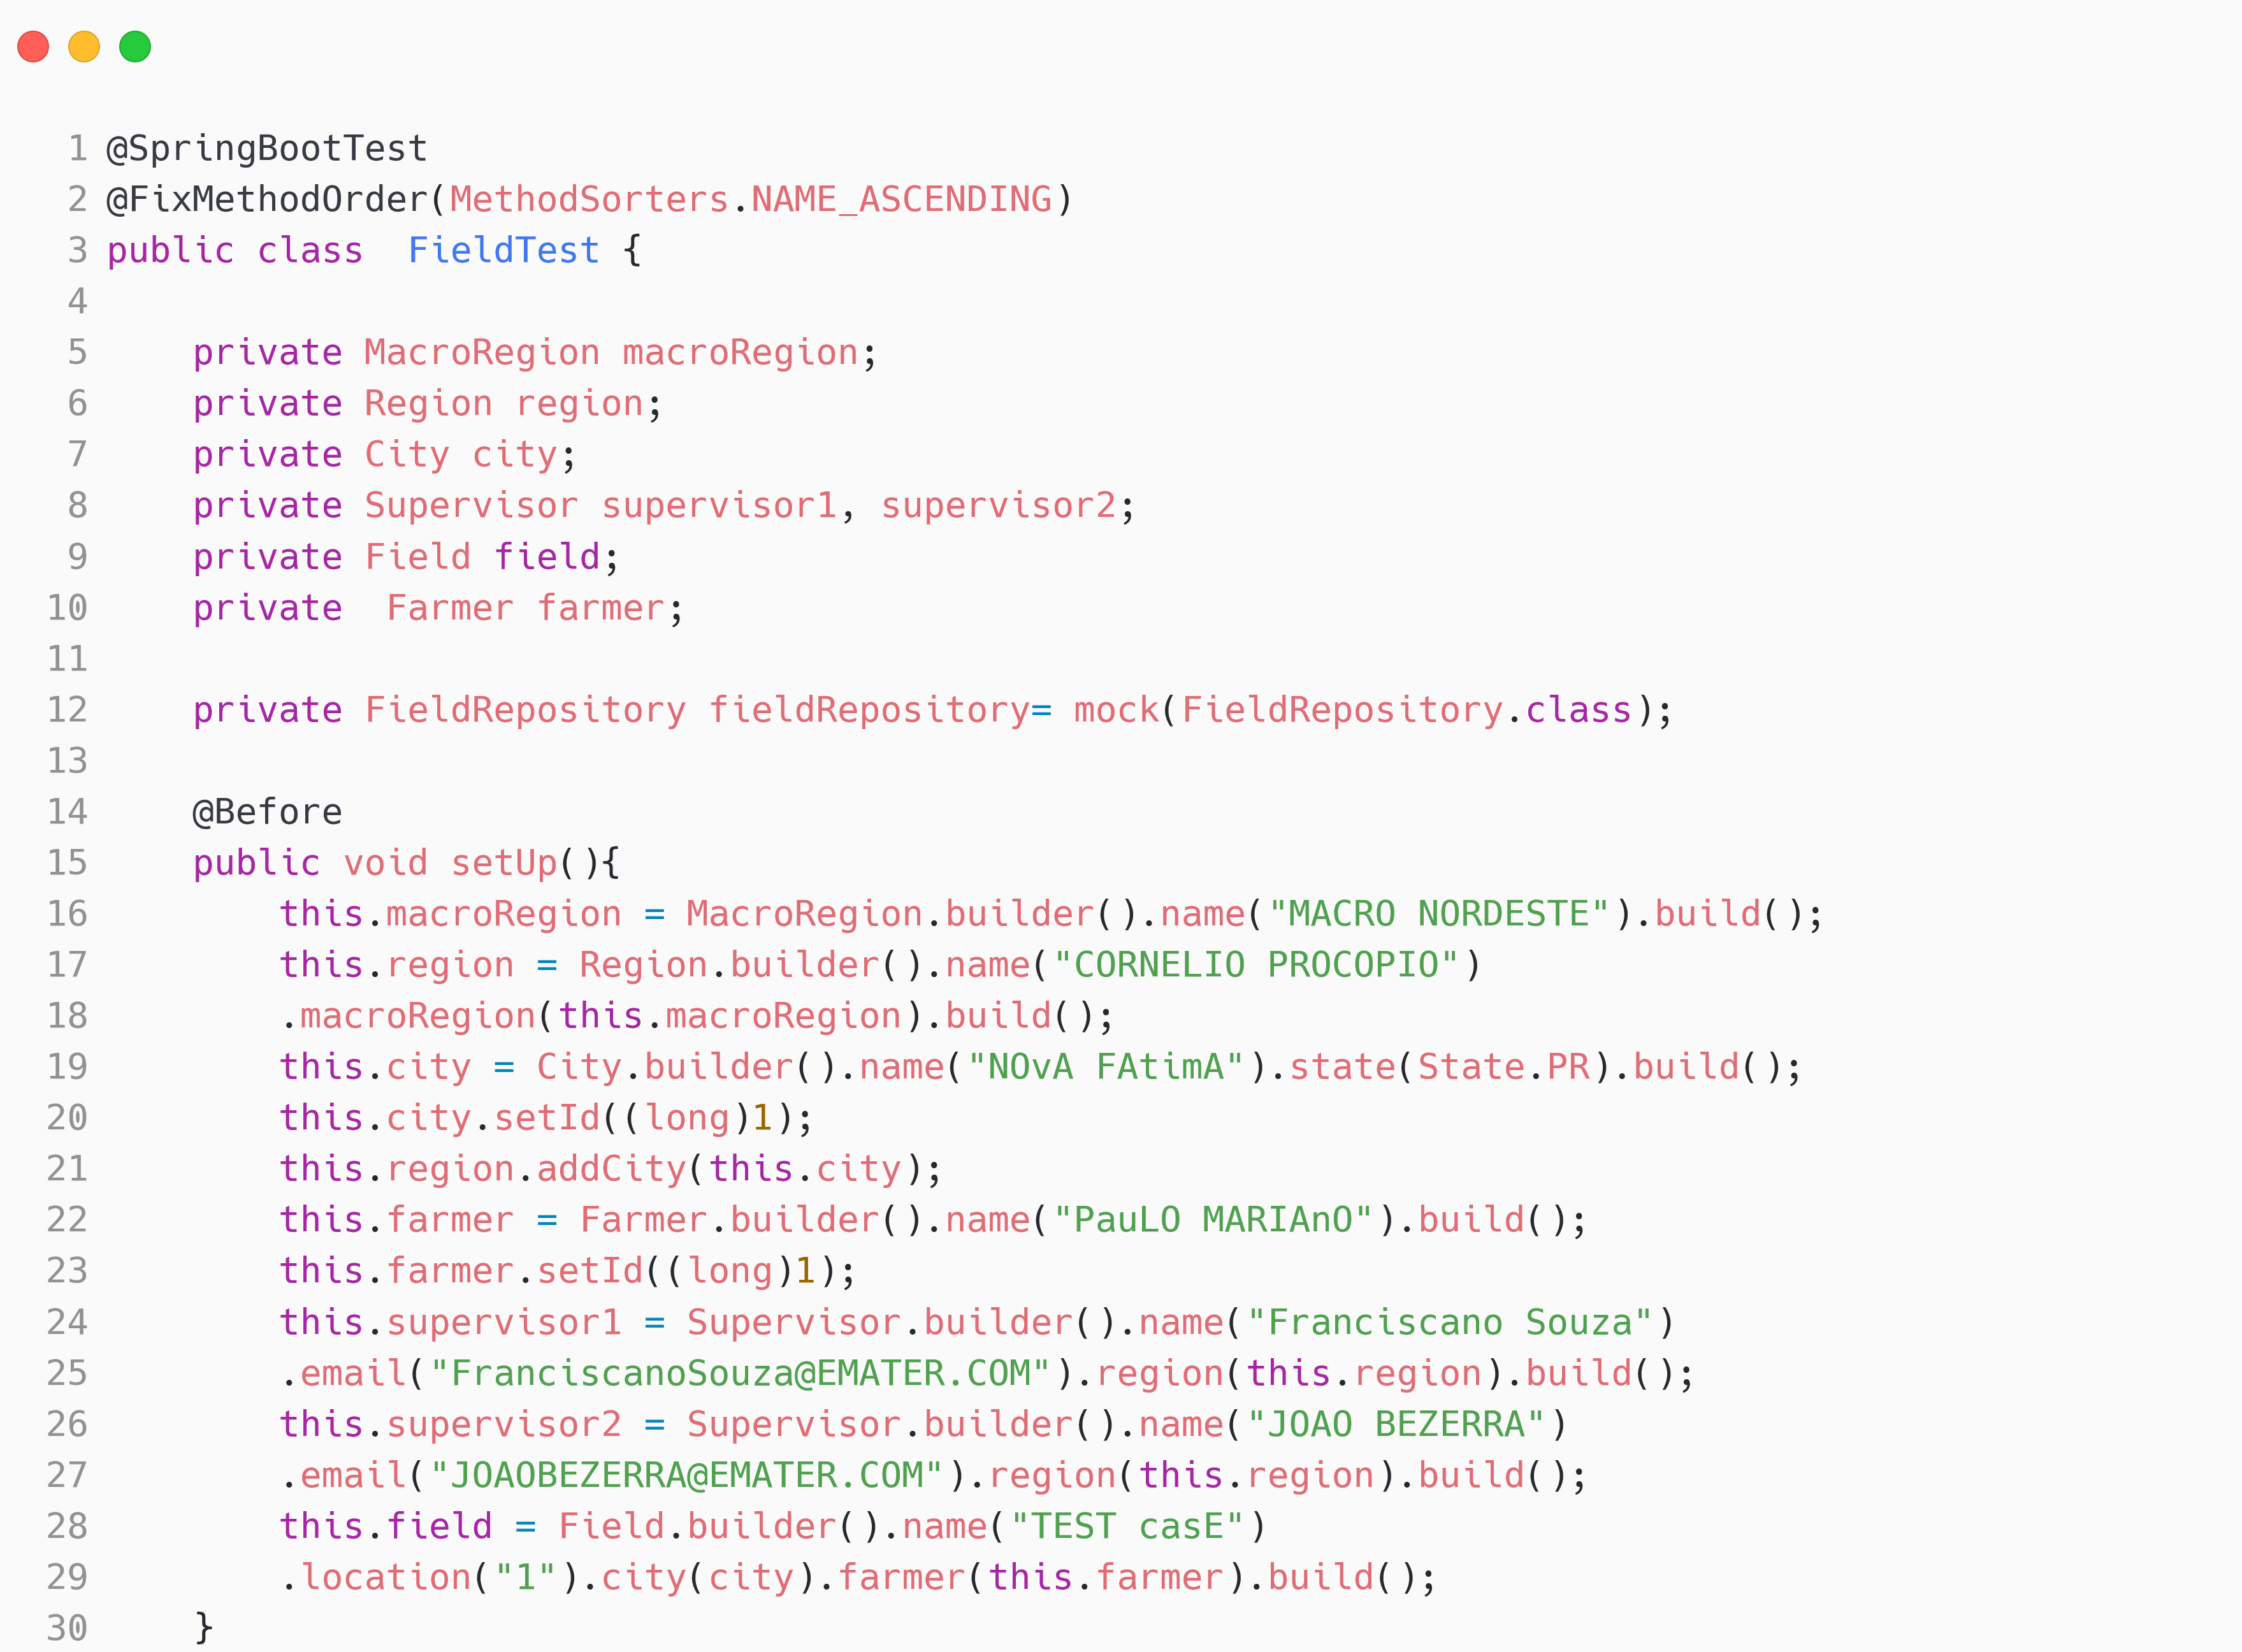
\includegraphics[scale=0.18]{dados/figuras/buildTestField.png}
\end{figure}

\begin{figure}[H]
	\centering
	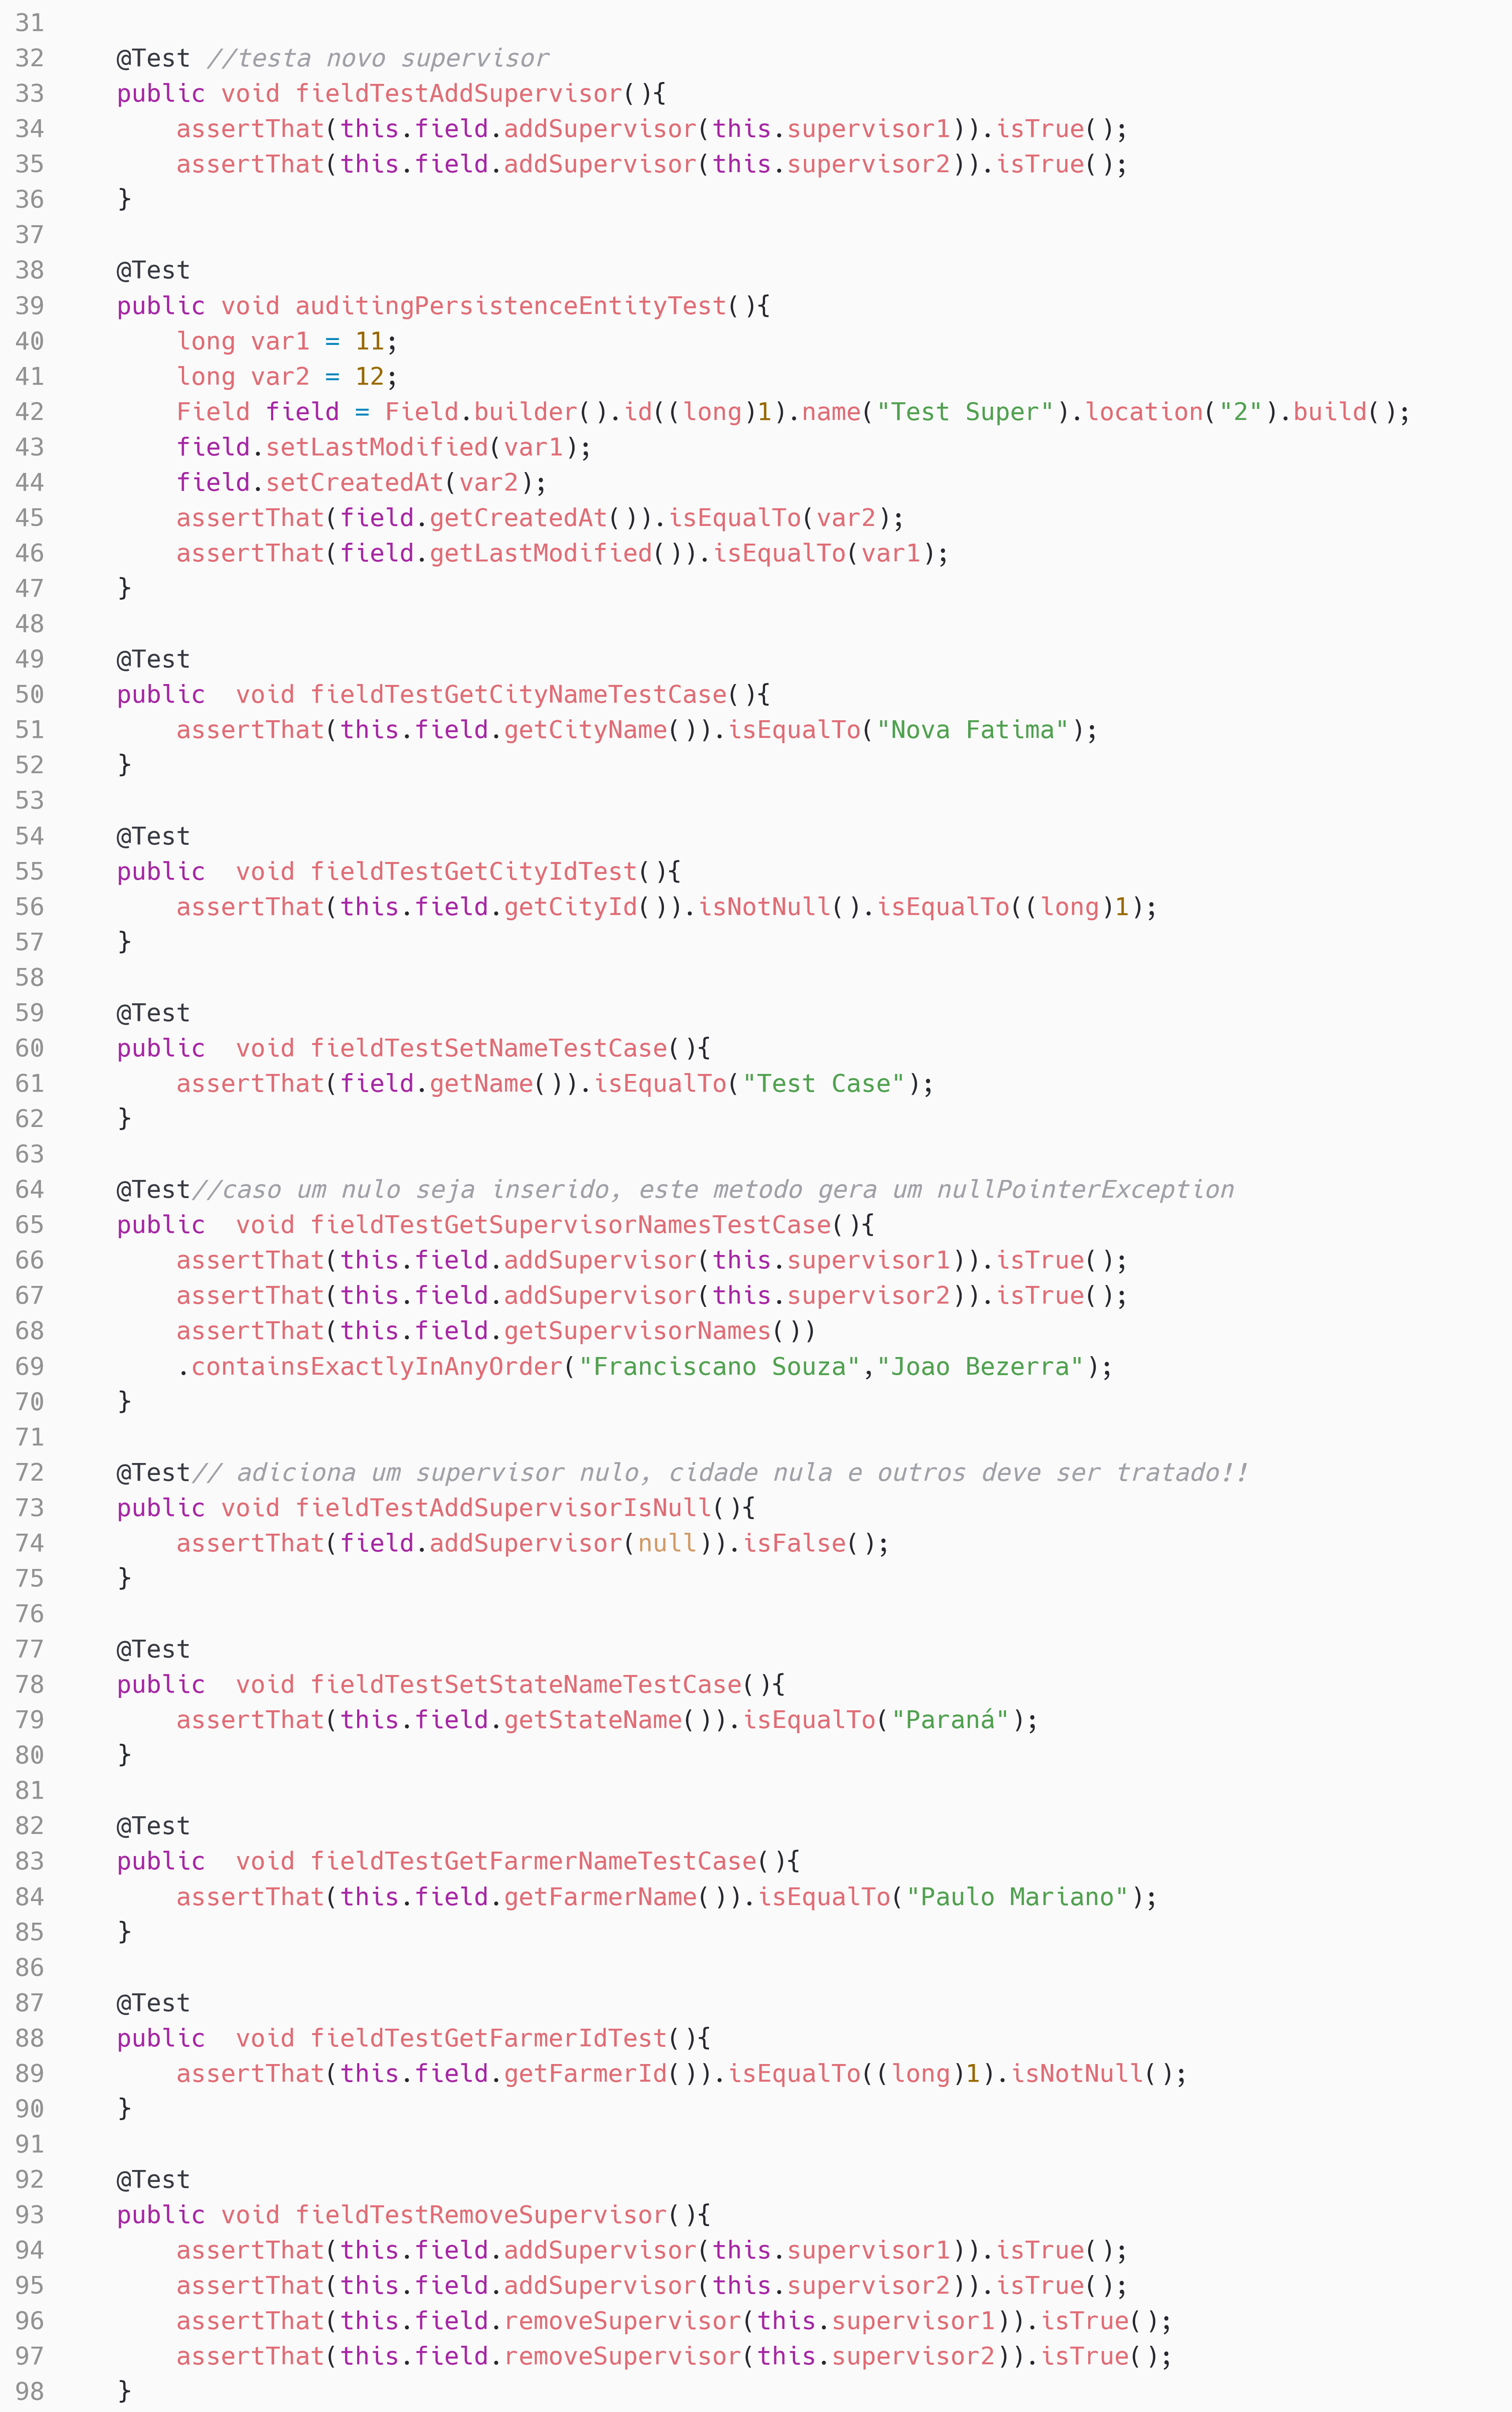
\includegraphics[scale=0.18]{dados/figuras/carbonField1.png}
\end{figure}

\begin{figure}[H]
	\centering
	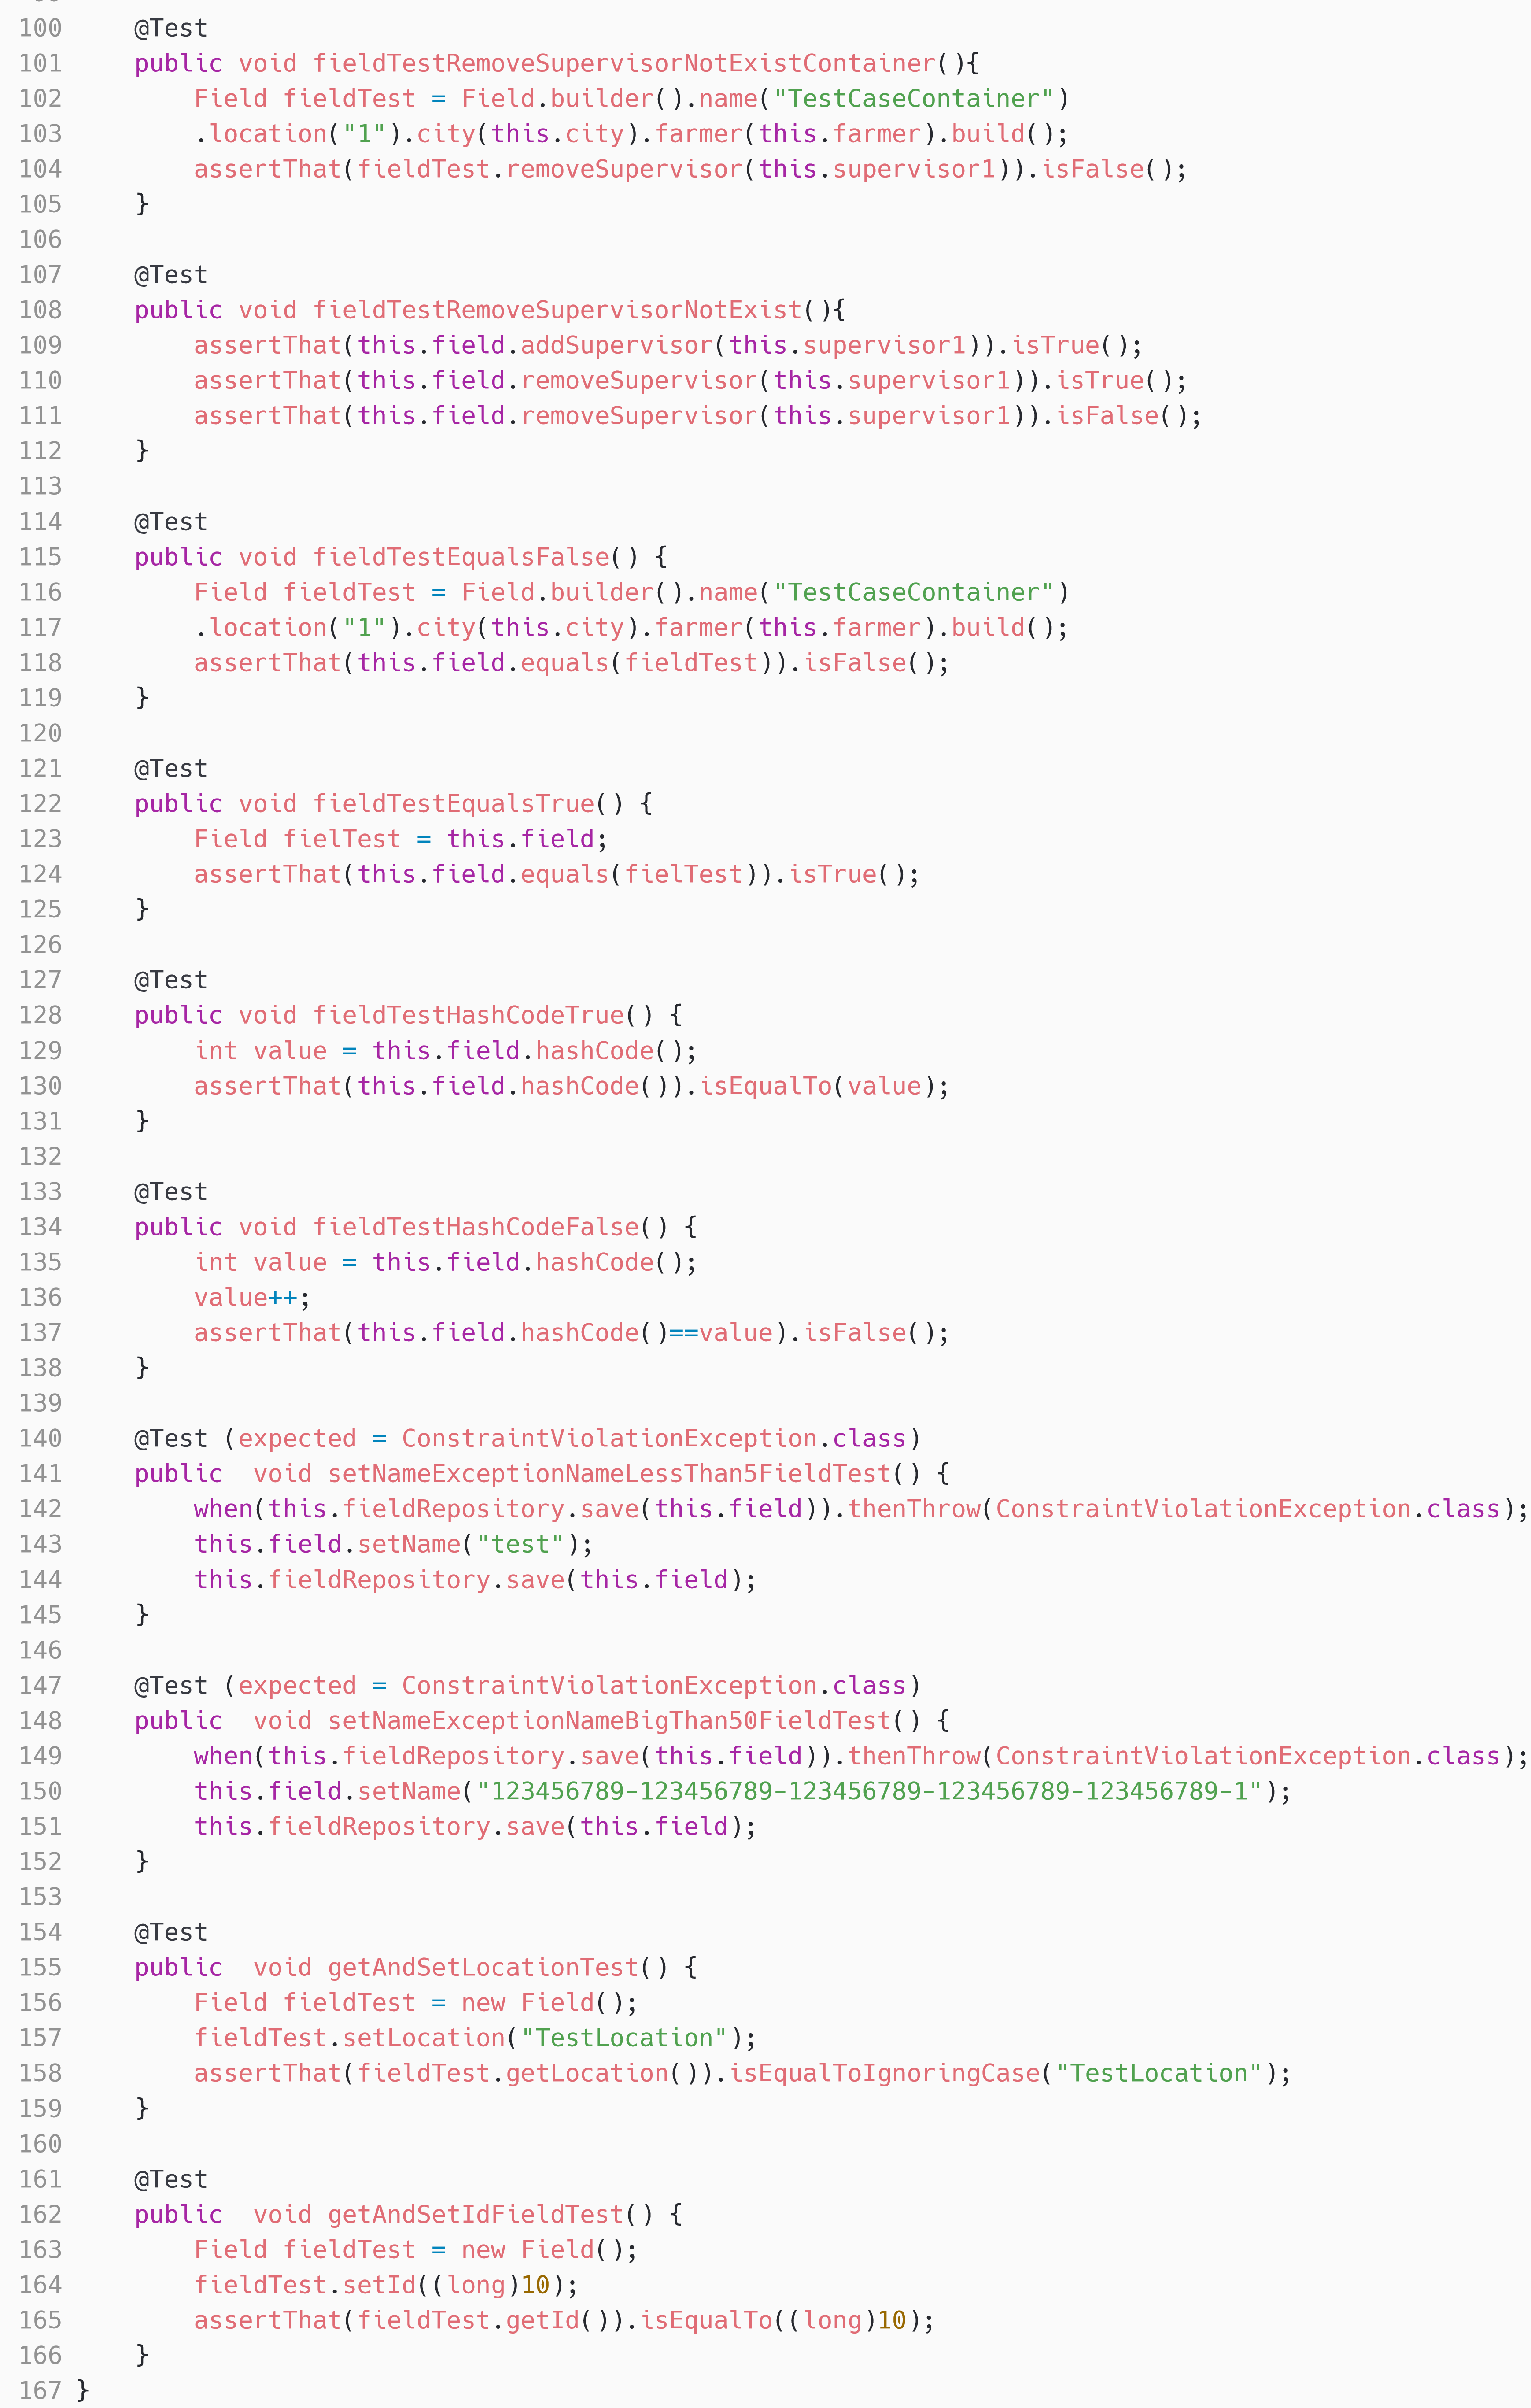
\includegraphics[scale=0.17]{dados/figuras/carbonField2.png}
	\caption{Classe de teste FieldTest.java.}
	\label{field1}
\end{figure}






Método de teste\textit{ “fieldTestGetSupervisorNamesTestCase()”} linhas 64 a 70 figura \ref{field1}: Este caso de teste verifica se o método\textit{ “Field.getSupervisorNames ()”} recupera os nomes de todos os supervisores adicionados ao objeto \textit{“Field”.} Os supervisores são criados nas linhas 24 a 27 e são adicionados a\textit{ “Field”} nas linhas 66 e 67. A entrada é composta por dois supervisores de nomes diferentes ("Franciscano Souza" e "Joao Bezerra"). O retorno do método testado consiste em uma lista do tipo \textit{“String”}, o teste verifica se a lista contem em qualquer ordem os elementos os elementos inseridos, o retorno é ("Franciscano Souza" e "Joao Bezerra");

Método de teste\textit{ “fieldTestAddSupervisorIsNull()”} linhas 72 a 75 figura \ref{field1}: Este caso de teste consiste em inserir um supervisor como\textit{ “null”}, caso o nulo seja inserido gera uma inconsistência pois outros métodos de consulta podem falhar. A entrada é um\textit{ “null”} linha 74, e o retorno esperado é um \textit{“FALSE”,} pois, a inserção não deve ser realizada, mas o retorno é um\textit{ “TRUE”} confirmando à inserção de um nulo como um supervisor. Esta inserção pode gerar uma inconsistência em consultas futuras.

Método de teste\textit{ “fieldTestSetStateNameTestCase ()”} linhas 64 a 70 figura \ref{field1}: Este teste consiste em recuperar o nome do estado a qual a cidade pertence. A Entrada consiste em um objeto do tipo \textit{“Estate.PR”} linha 19. O retorno esperado é uma \textit{string} de caracteres contendo “Paraná”. O retorno do método testado é uma \textit{string} contendo “Paraná”   

Método de teste \textit{“fieldTestGetFarmerNameTestCase ()”} linhas 82 a 85 figura \ref{field1}: Este meto busca o nome do agricultor atribuído ao objeto\textit{ “Field”}. A entrada consiste em um objeto do tipo\textit{ “Farme” }com o atributo nome definido como “PauLO MARIAnO” linha 22. O retorno do método testado deve ser uma \textit{string} contendo o nome do agricultor formatado com a primeira letra de cada palavra maiúscula. O retorno do teste linha 84 é uma \textit{string} que contem “Paulo Mariano”.


Método de teste\textit{ “fieldTestGetFarmerIdTest ()”} linhas 87 a 90 figura \ref{field1}: Este método consiste em recuperar o atribuo identificador de agricultor a entrada é feita na linha 23 sendo o valor (\textit{long} 1). O retorno do método testado deve ser um \textit{long} contendo o identificador único do agricultor. O retorno do meto é um tipo \textit{long} contendo o valor 1. 


Método de teste \textit{“fieldTestRemoveSupervisor ()”} linhas 92 a 98 figura \ref{field1}: Este teste consiste em atribuir novos supervisores a um objeto\textit{ “Field”} e em seguida remove-los. A entrada consiste em dois supervisores linhas 94 e 95. A saída consiste em um\textit{ “boolean”} para cada remoção\textit{, “TRUE”} caso o supervisor seja removido, e\textit{ “FALSE”} caso o supervisor não seja removido.  A sida nesse teste é\textit{ “TRUE”} para as duas execuções pois os dois supervisores enviados para remoção foram encontrados.

Método de teste\textit{ “fieldTestRemoveSupervisorNotExistContainer ()”} linhas 100 a 105 figura \ref{field1}: Este caso de teste consiste em tentar remover um supervisor de um objeto \textit{“Field” }sem que não haja um container do tipo supervisor criado em\textit{ “Field”}. A entrada consiste em um supervisor não pertencente ao objeto \textit{“FieldTest”} criado na linha 102. A saída nesse caso de teste é um\textit{ “FALSE”} pois ainda não foi inserido nenhum supervisor a \textit{“FieldTest”}.
 
Método de teste \textit{“fieldTestRemoveSupervisorNotExist()” }linhas 107 a 112 figura \ref{field1}: Este método consiste em testar a remoção de um supervisor que já foi removido anteriormente. A entrada consiste em um supervisor linhas 109. A saída consiste em \textit{“TRUE”} caso os objetos sejam removidos com sucesso, saída apresentada na linha 110 ou \textit{“FALSE”} caso o supervisor já não exista mais em\textit{ “Field” }saída apresentada na linha 111.

Método de teste\textit{ “fieldTestEqualsFalse()”} linhas 114 a 119 figura \ref{field1}: Este método de teste consiste em comparar dois objetos do tipo\textit{ “Field”} caso eles sejam iguais o retorno é um\textit{ “boolean” “TRUE”} caso sejam diferentes o retorno é um\textit{ “FALSE”}. A entrada consiste em dois objetos do tipo\textit{ “Field”}, o primeiro objeto é criado nas linhas 28 e 29, o segundo objeto é criado nas linhas 116 e 117. A saída é um \textit{“FALSE” }pois os objetos comparados são diferentes.

Método de teste \textit{“fieldTestEqualsTrue()” }linhas 121 a 125 figura \ref{field1}: Este método de teste consiste em comparar dois objetos do tipo\textit{ “Field”} caso eles sejam iguais o retorno é um \textit{“boolean” “TRUE”} caso sejam diferentes o retorno é um\textit{ “FALSE”}. A entrada consiste em dois objetos do tipo \textit{“Field”,} o primeiro objeto é criado nas linhas 28 e 29, o segundo objeto é criado nas linhas 116 e 117 e recebe uma cópia do objeto criado anteriormente. A saída é um \textit{“TRUE” }pois os objetos são iguais.

Método de teste \textit{“fieldTestHashCodeTrue()” }linhas 127 a 131 figura \ref{field1}: Este teste consiste em recuperar o valor de \textit{“hashcode” }de um objeto e verifica seu valor em uma segunda chamada. O método não possui entrada. A saída consiste em um valor numérico do tipo \textit{“int”.} O valor de \textit{hash} é recuperado em uma primeira chamada na  linha 129. em seguida é feita uma assertiva, esta compara o valor recuperado anteriormente com o valor de uma nova chamda do método de \textit{hash}, os valores são iguais.

Método de teste\textit{ “fieldTestHashCodeFalse()”} linhas 133 a 138 figura \ref{field1}: Este teste consiste em recuperar o valor de\textit{ “hashcode”} de um objeto e verifica seu valor em uma segunda chamada. O método não possui entrada. A saída consiste em um valor numérico do tipo \textit{“int”.} O valor de \textit{hash} é recuperado em uma primeira chamada na linha 135, em seguida é feito um incremento no valor recuperado. Uma assertiva compara o valor chamado anteriormente e incrementado com o valor de uma nova chamda do método de \textit{hash}, os valores são diferentes..

Método de teste \textit{“setNameExceptionNameLessThan5FieldTest()”} linhas 140 a 145 figura \ref{field1}: Uma das restrições que se encontra na hora de salvar um objeto do tipo \textit{“Field” }é que a variável\textit{ “name”} do tipo \textit{“String” }deve ter entre 5 e 50 caracteres. A entrada consiste em uma\textit{ “String”} contendo apenas quatro caractere. A saída esperada é uma exceção de violação das regras do banco. A saída deste teste é uma \textit{“ConstraintViolationException.class” }disparada pelo\textit{ “FieldRepository.class”} pois o valor atribuído é menor que a regra estipulado.

Método de teste \textit{“setNameExceptionNameBigThan50FieldTest()”} linhas 147 a 152 figura \ref{field1}: Uma das restrições que se encontra na hora de salvar um objeto do tipo\textit{ “Field”} é que a variável \textit{“name”} do tipo\textit{ “String”} deve ter entre 5 e 50 caracteres. A entrada consiste em uma \textit{“String” }contendo apenas cinquenta e um caractere. A saída esperada é uma exceção de violação das regras do banco. A saída deste teste é uma\textit{ “ConstraintViolationException.class”} disparada pelo\textit{ “FieldRepository.class”} pois o valor atribuído é maior que a regra estipulado.

Método de teste \textit{“getAndSetLocationTest()”} linhas 154 a 159 figura \ref{field1}: Este teste consistem em atribuir um valor de localização para o objeto \textit{“Field”} e recuperar este valor posteriormente. O valor de entrada consiste em uma string “\textit{TestLocation}”. O valor recuperado no teste é uma string “\textit{TestLocation}”.

Método de teste \textit{“getAndSetIdFieldTest()”} linhas 161 a 166 figura \ref{field1}: Este teste consiste em atribuir um valor de identificação a um objeto\textit{ “Field”} e posteriormente recuperar este valor. O valor de entrada é um “\textit{long} 10”. O valor recuperado no teste é um “\textit{long} 10”.

Após a execução dos testes a cobertura das entradas e saídas de dados da classe Field.java é de 100\%. 


\subsection{RESULTADO DOS TESTES CLASSE SURVEY.JAVA}

Outra classe que tem grande importância no sistema é a \textit{Survei.java}, várias outras classes a compõem poies é ela que registra os dados de produção de uma colheita de um agricultor. A FIGURA \ref{classesSurvey} apresenta o diagrama de classes que compõem a classe \textit{Survey} e exibe a classe \textit{SurveyTest} que testa os métodos e atributos  da classe \textit{Survey}.


\begin{figure}[H]
	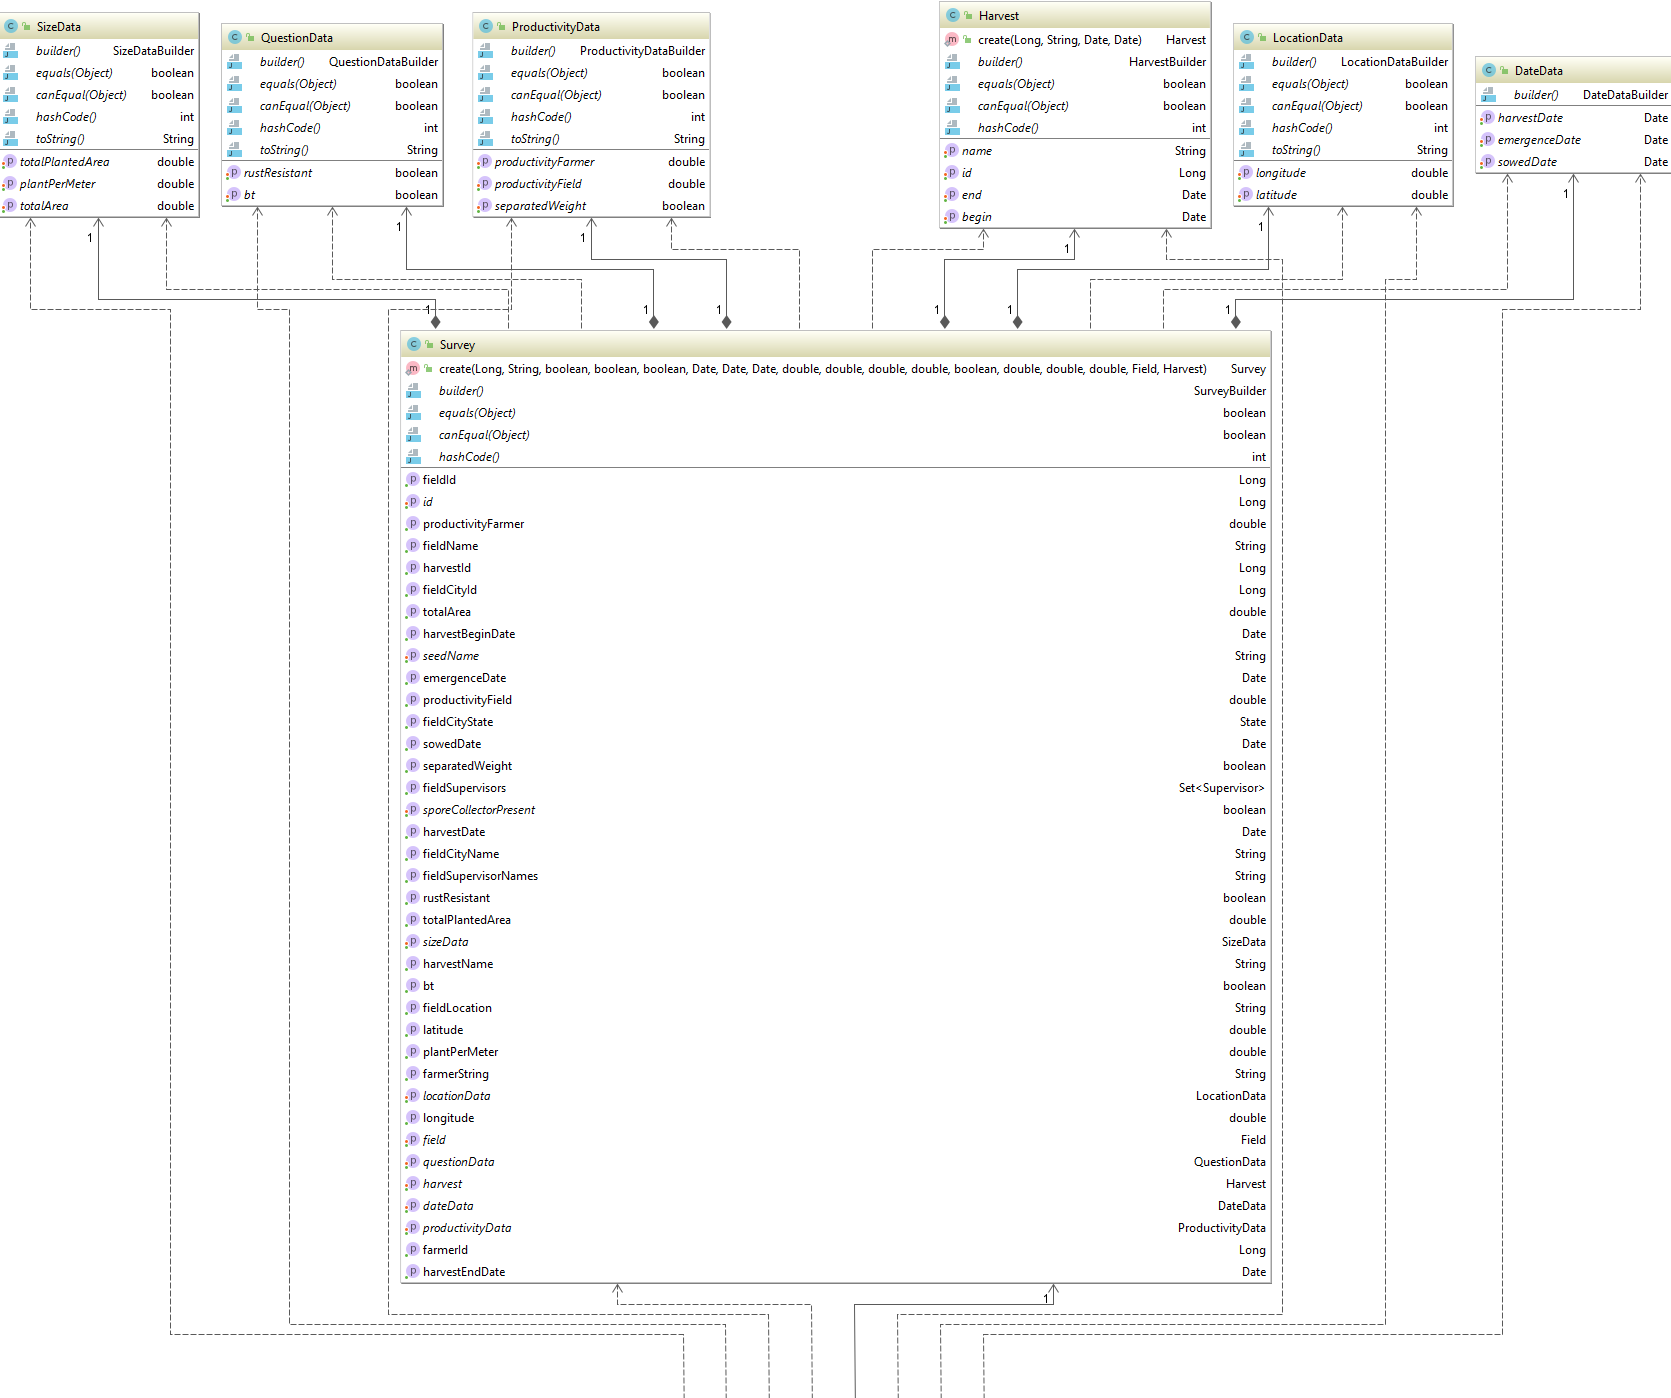
\includegraphics[scale=0.38]{dados/figuras/packSurvei.png}
\end{figure}

\begin{figure}[H]
	\centering
	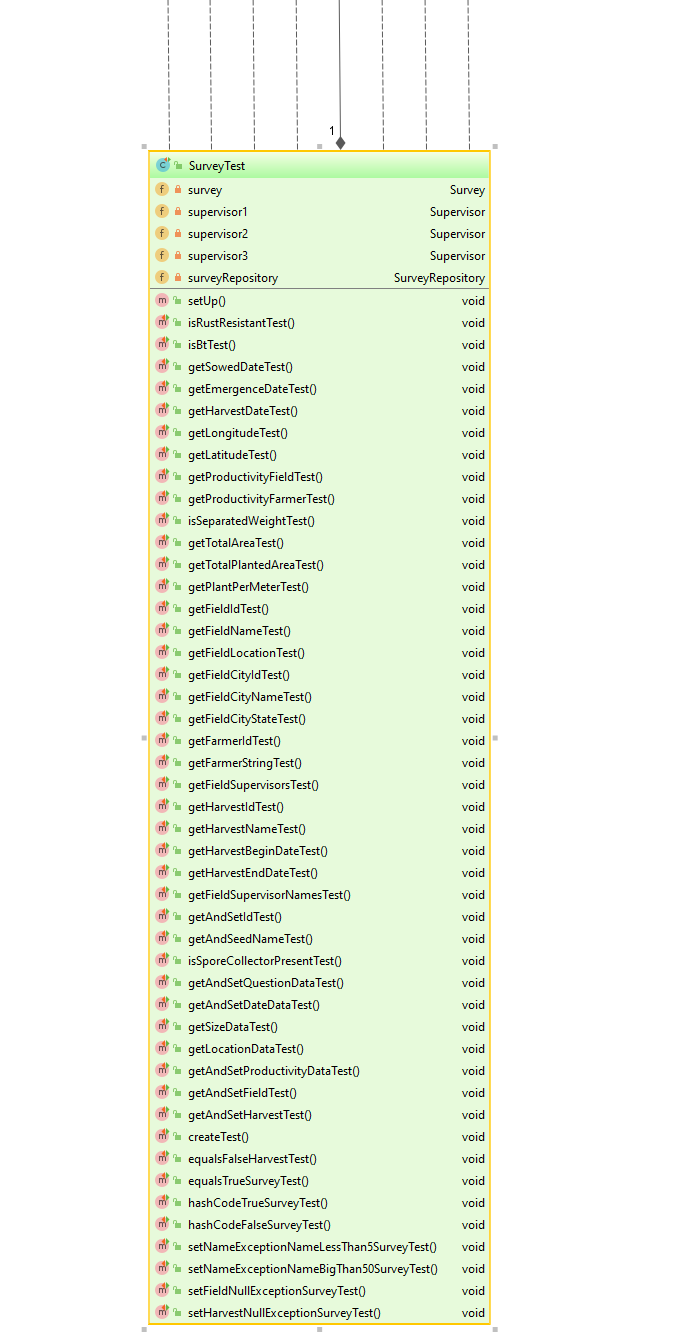
\includegraphics[scale=0.7]{dados/figuras/surveyTest.png}
	\caption{Diagrama de classes Survey e SurveyTest.java.}
	\label{classesSurvey}
\end{figure}

A classe de teste apresentada na FIGURA \ref{classesSurvey} possui 46 métodos de teste é um método de apoio aos testes denominado \textit{“setUp”}, o objetivo dos testes é exercitar a classe \textit{Survey} até que todos as variáveis, entradas e saídas de dados sejam executados pelo menos uma vez. Como a classe \textit{Survey} é composta por outras classes se faz necessário a instanciação de outras classes como \textit{Harvest}, \textit{Farmer}, \textit{City}, \textit{SizeData} e outras para a execução completa dos testes. Como a classe se trata de uma entidade que será persistida em um banco de dados, ela possui certas regras de negócio que serão ativadas somente no momento de gravar os dados no banco, sendo assim foi preciso criar uma referência para a interface \textit{SurveyRepository}, classe responsável por realizar a persistência dos dados no banco. Como o objetivo deste trabalho é cobrir o sistema com testes unitários e testes que integram classes entidades com o banco de dados ou comunicação com \textit{APIs} são testes de integração foi utilizado um \textit{“Mock”} para simular o comportamento do repositório.


A FIGURA \ref{testSurvey} apresenta a declaração da classe de teste, os atributos utilizados para desenvolver os testes e o método \textit{“setUp”} utilizado para preparar o ambiente para os testes.

O trecho de código da FIGURA \ref{testSurvey} apresenta as seguintes funcionalidades:

\begin{itemize}

    \item Na linha 1 é utilizada a anotação \textit{@FixMethodOrder} que permite definir uma ordem de execução dos testes, neste casso foi definida a ordem \textit{“NAME\_ASCENDING"} que faz a execução dos testes de acordo com o nome de maneira ascendente;
    
    \item Linha 2 a classe \textit{SurveyTest} é aberta;

    \item Na linha 4 é feita a declaração do objeto \textit{Survey}, nas linhas 5, 6 e 7  são declarados e instanciados objetos do tipo \textit{Supervisor};

    \item Na linha 8 um objeto do tipo \textit{SurveyRepositorio} é declarado e instanciado como um objeto \textit{mock};

    \item Na linha 10 é utilizado a anotação \textit{@Before}, esta anotação determina que sempre antes da execução de um teste o método \textit{“setUp”} deve ser executado primeiro.

    \item O método \textit{“setUp”} que tem sua declaração na linha 11 e vai até a linha 32, ele é responsável por realizar a construção do objeto \textit{Survey} declarado na linha 4.

\end{itemize}{}


A FIGURA \ref{testSurvey} apresenta os casos de testes criados para a classe \textit{Survey}. 


A ideia geral na elaboração dos testes é a de cobrir cada atribuição de dados, as entrada e saída de dados da classe \textit{Survey}, buscando a cobertura de 100\% das linhas métodos e atributo da classe. Os resultados obtidos da execução dos testes foram listados a seguir:



\begin{figure}[H]
	\centering
	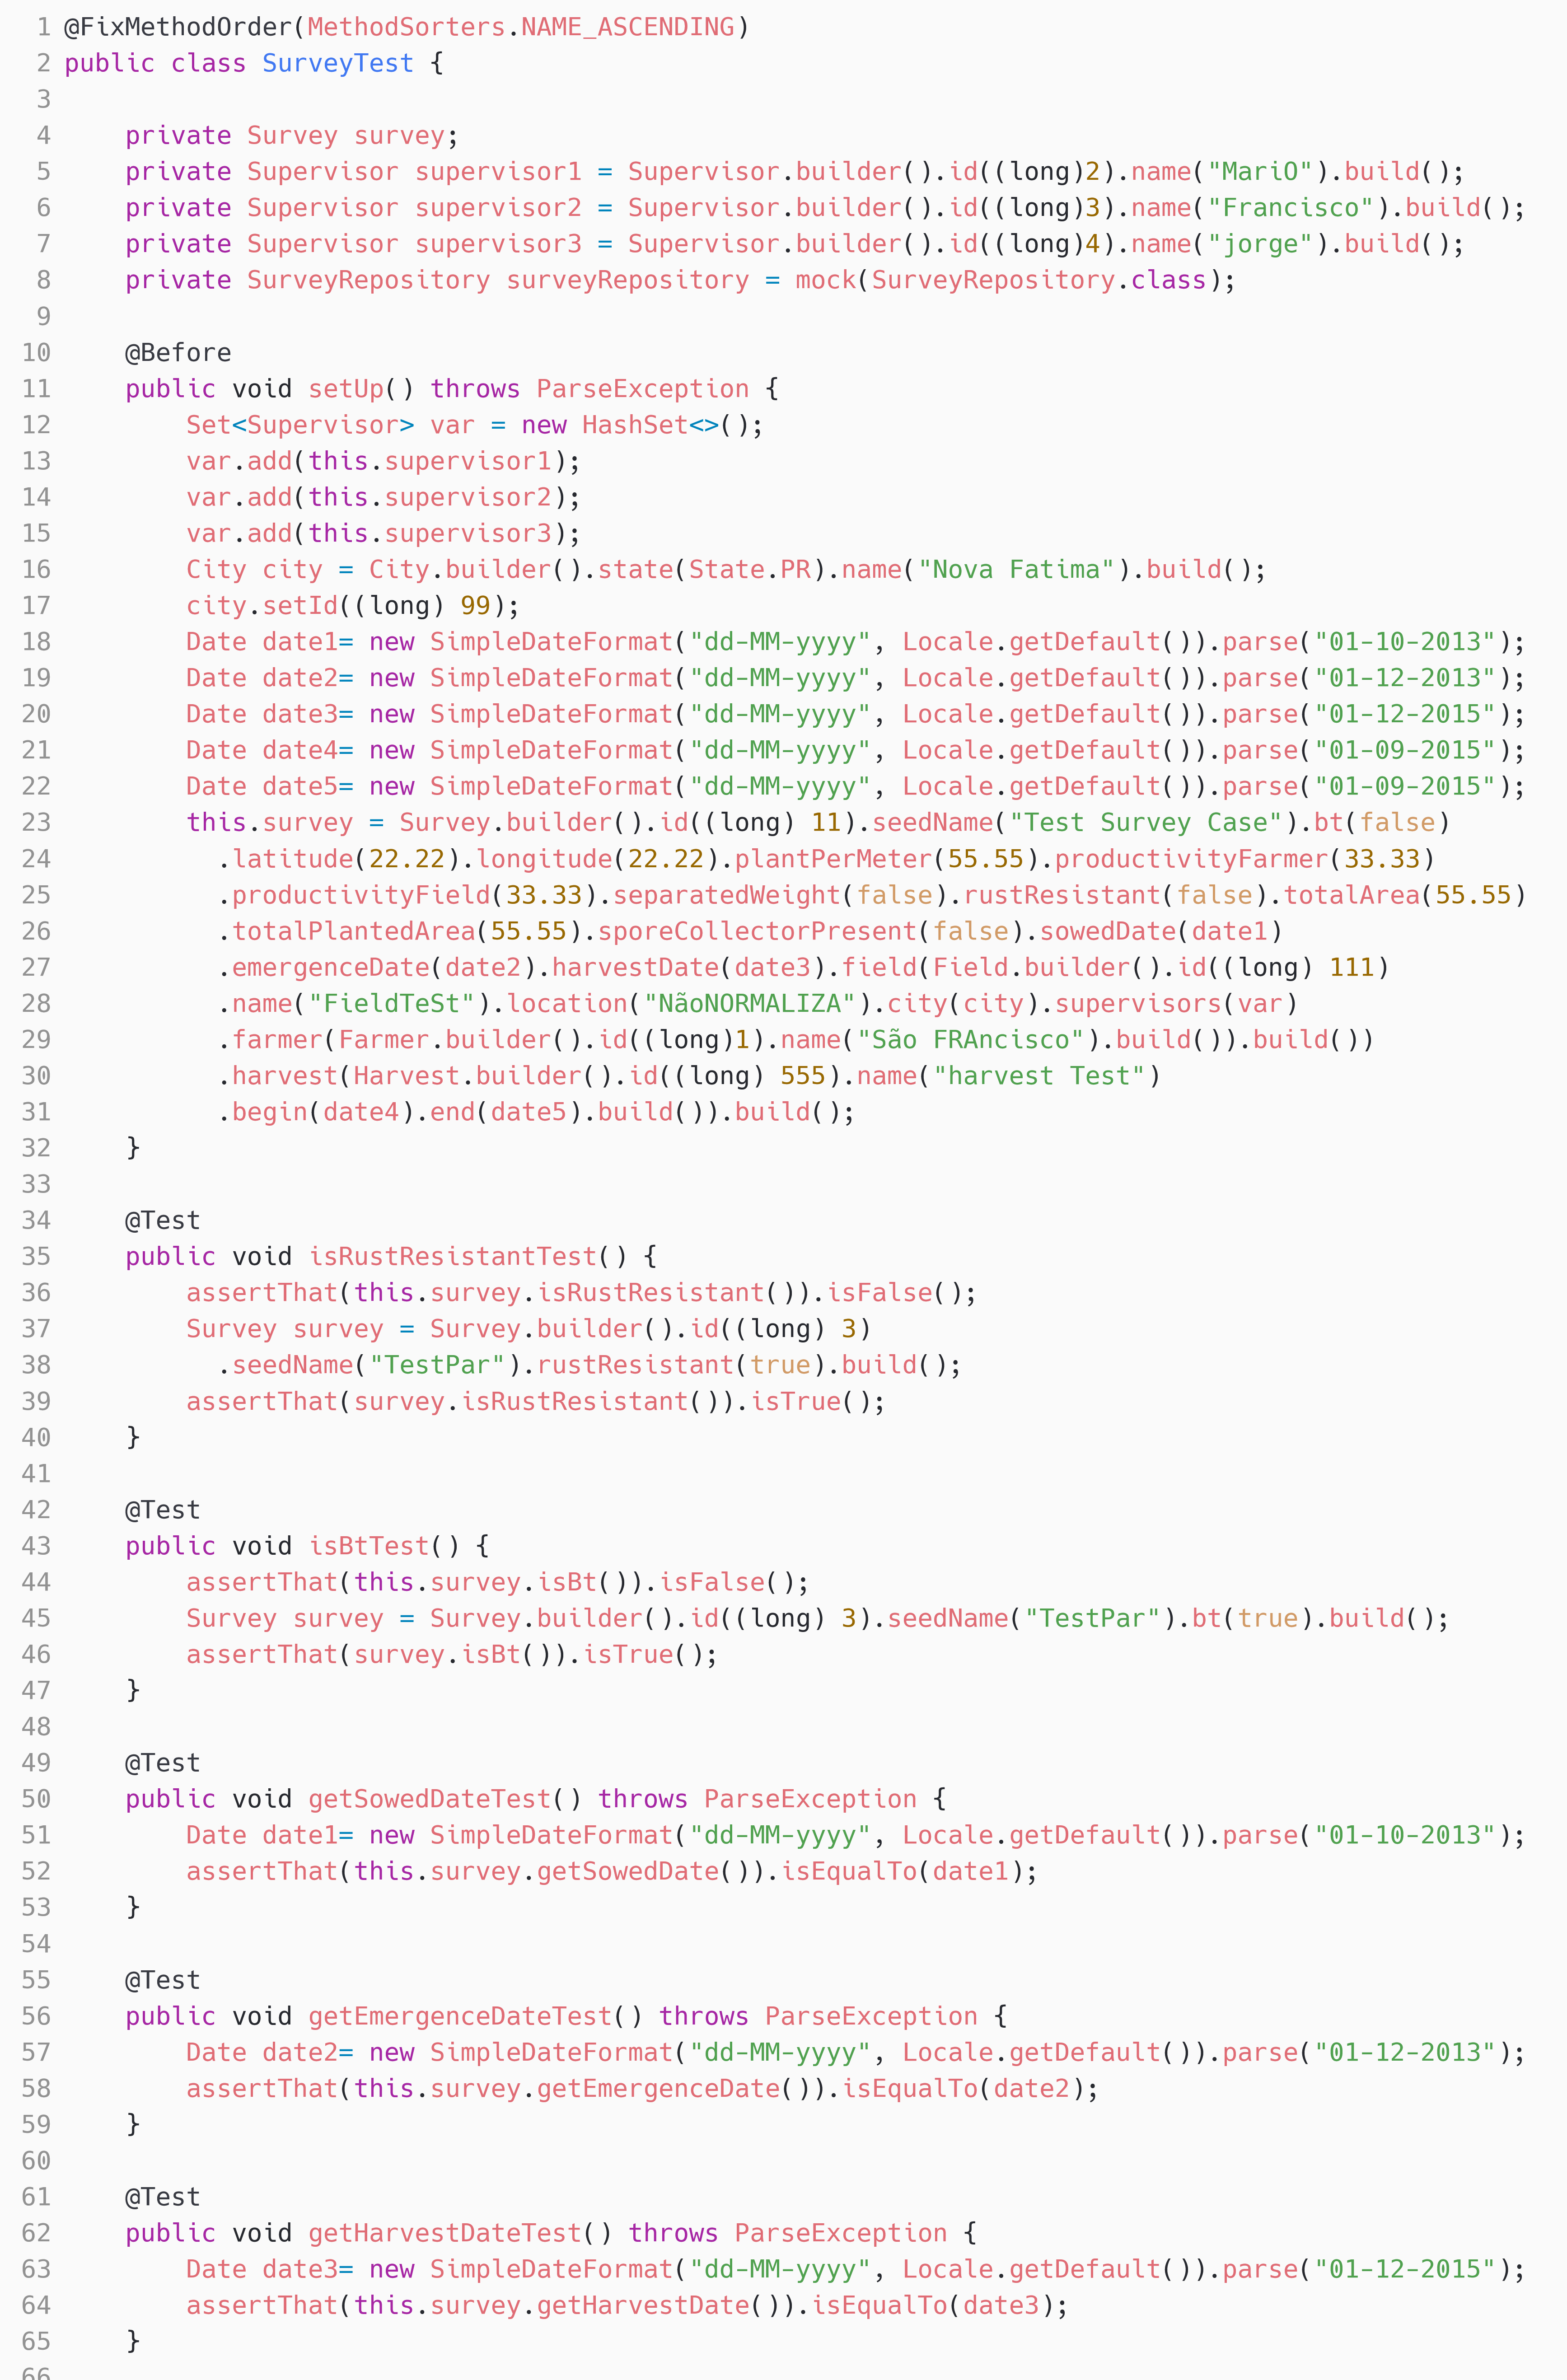
\includegraphics[scale=0.17]{dados/figuras/buildSurvey.png}
\end{figure}

\begin{figure}[H]
	\centering
	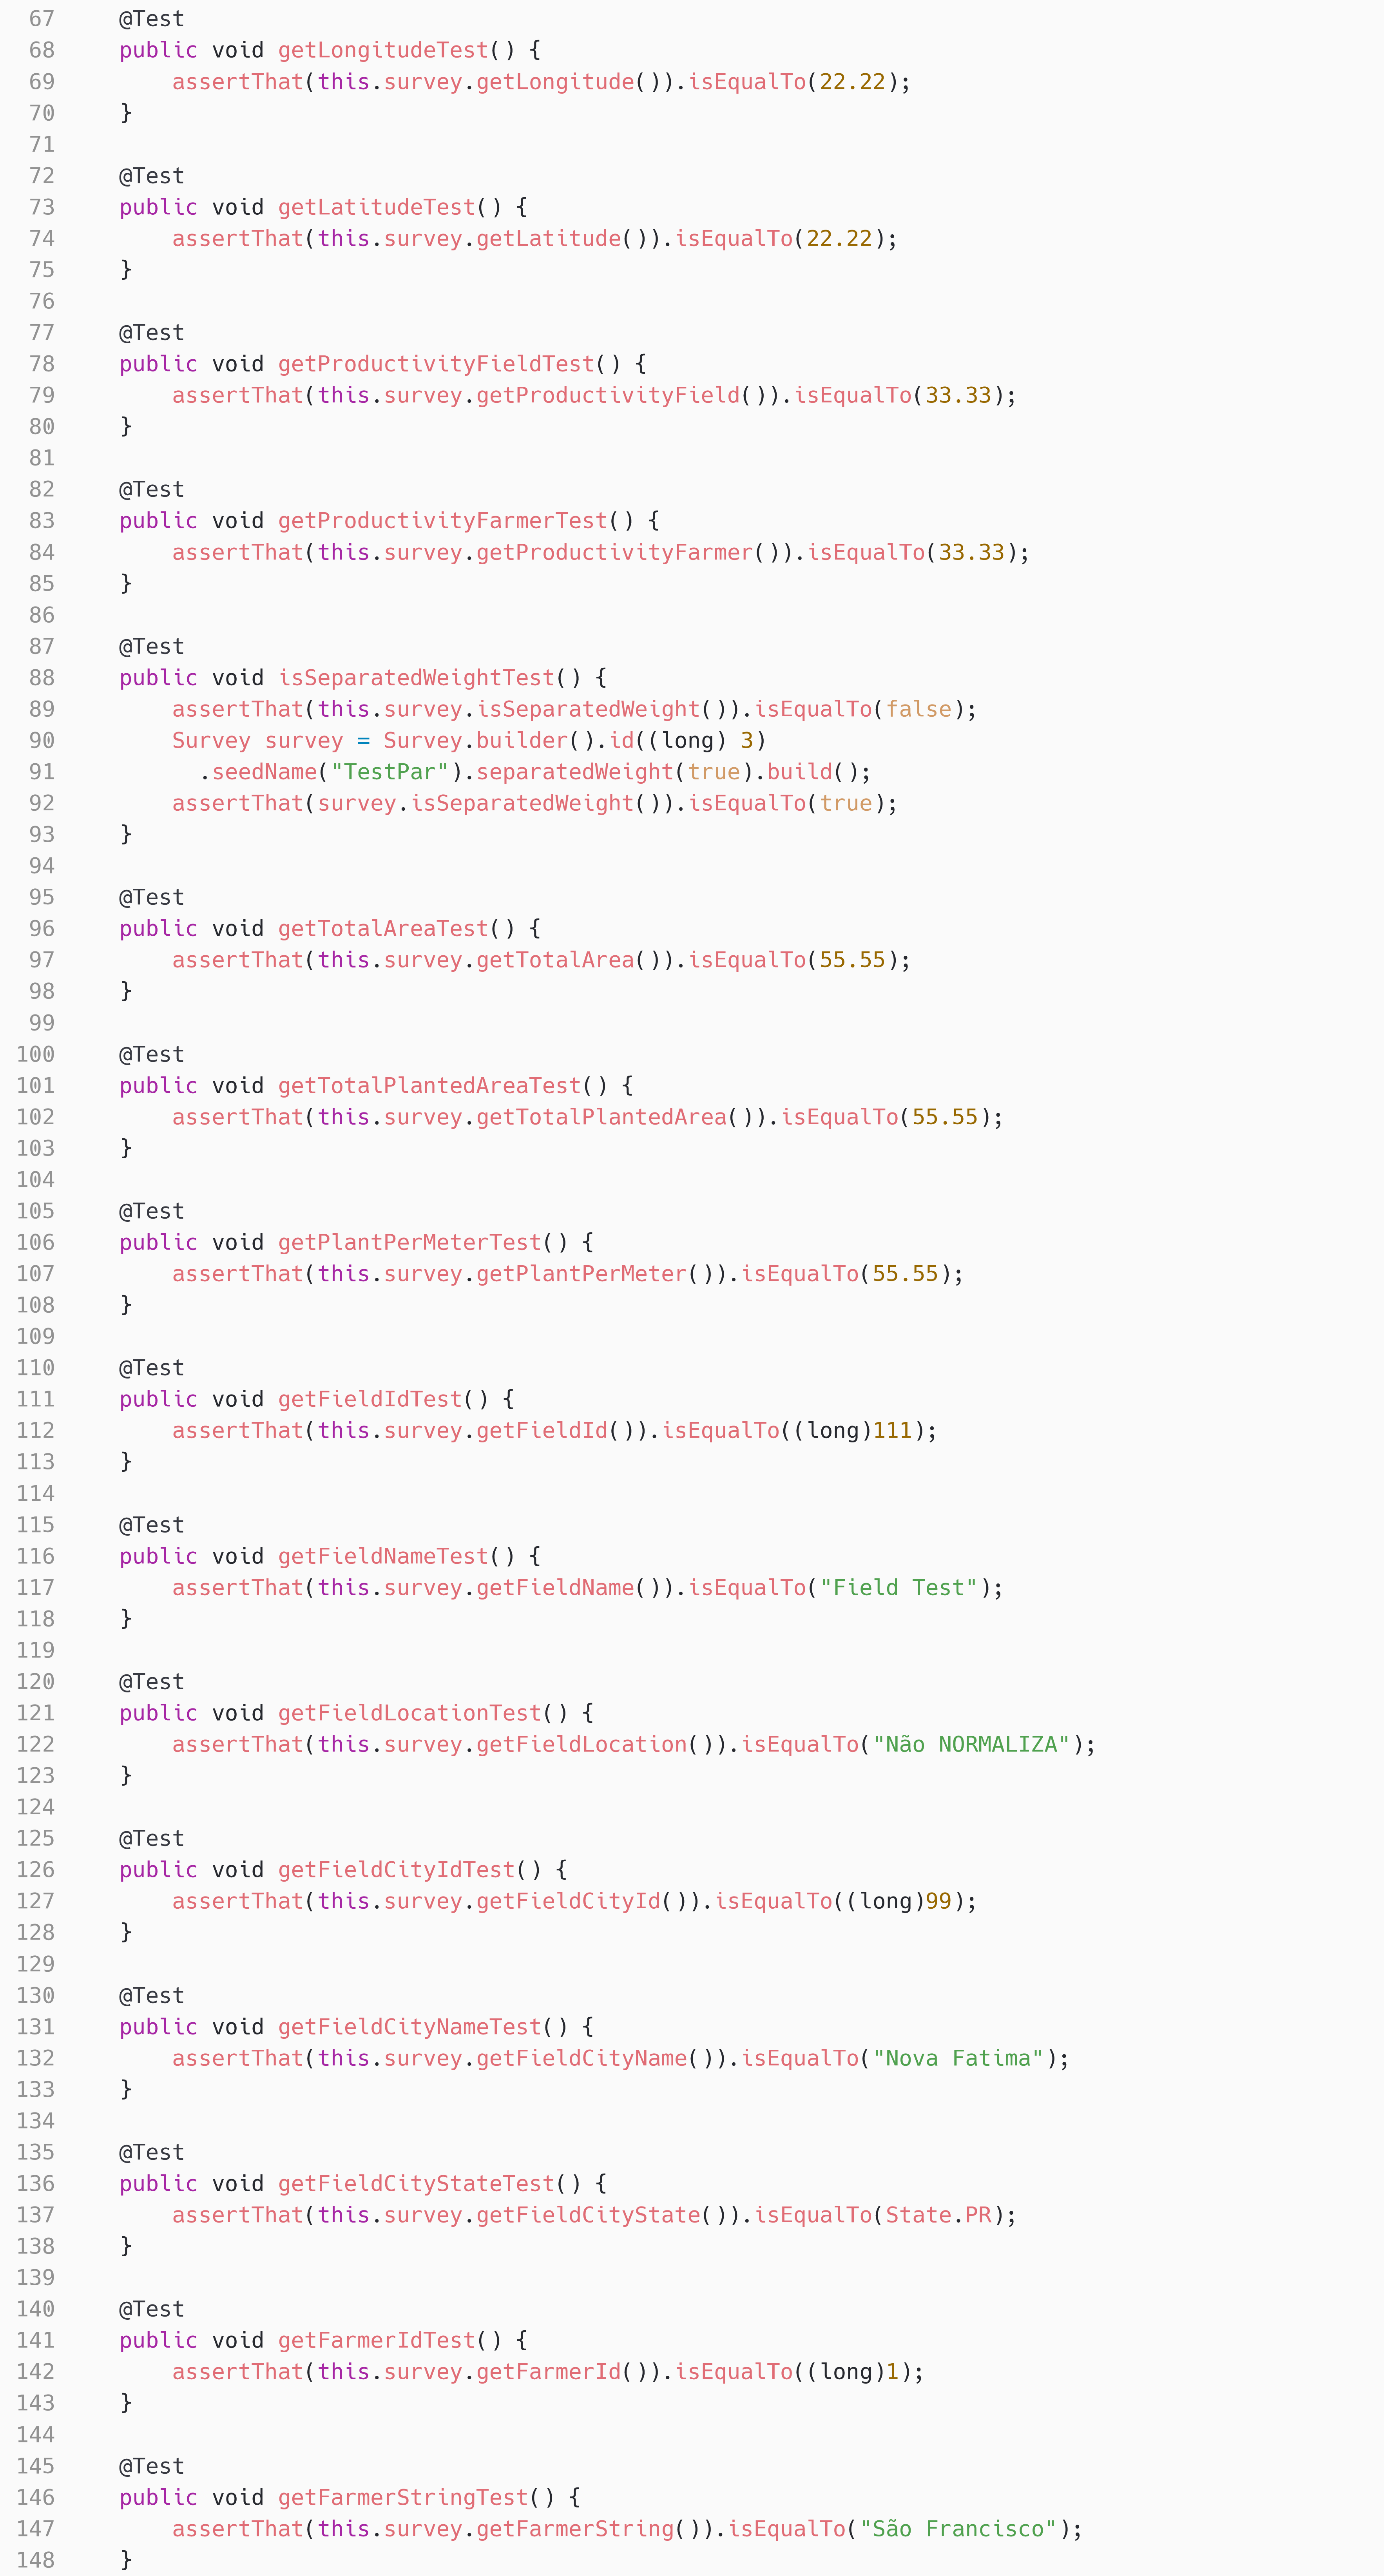
\includegraphics[scale=0.14]{dados/figuras/surveyTest1.png}
\end{figure}

\begin{figure}[H]
	\centering
	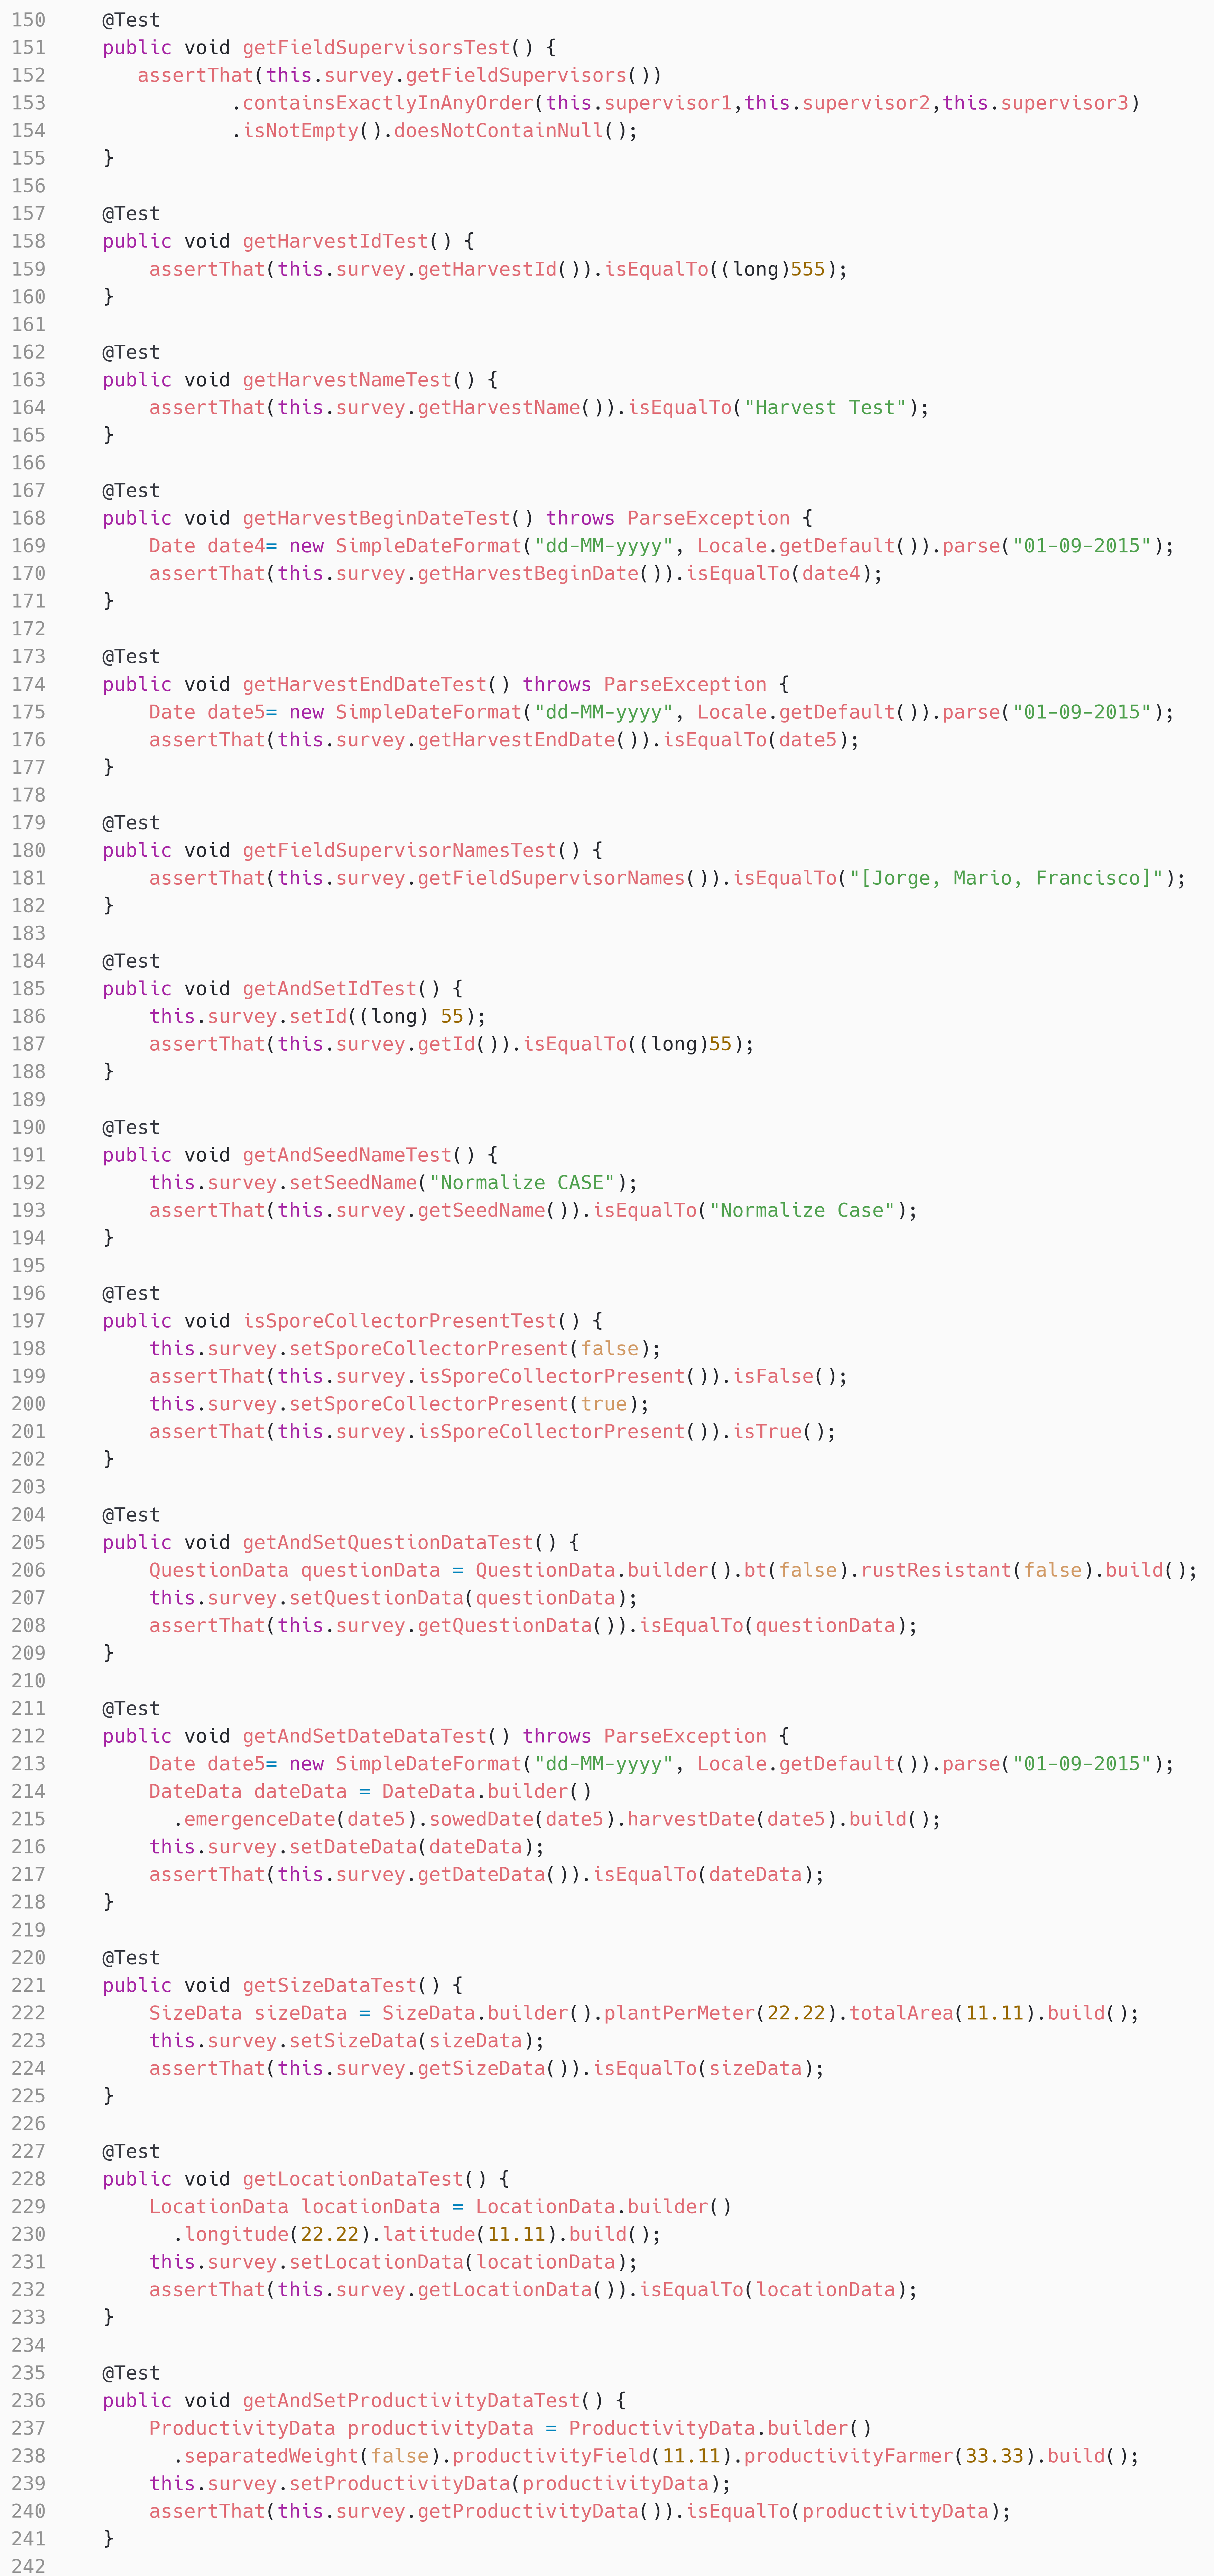
\includegraphics[scale=0.13]{dados/figuras/surveyTest2.png}
\end{figure}

\begin{figure}[H]
	\centering
	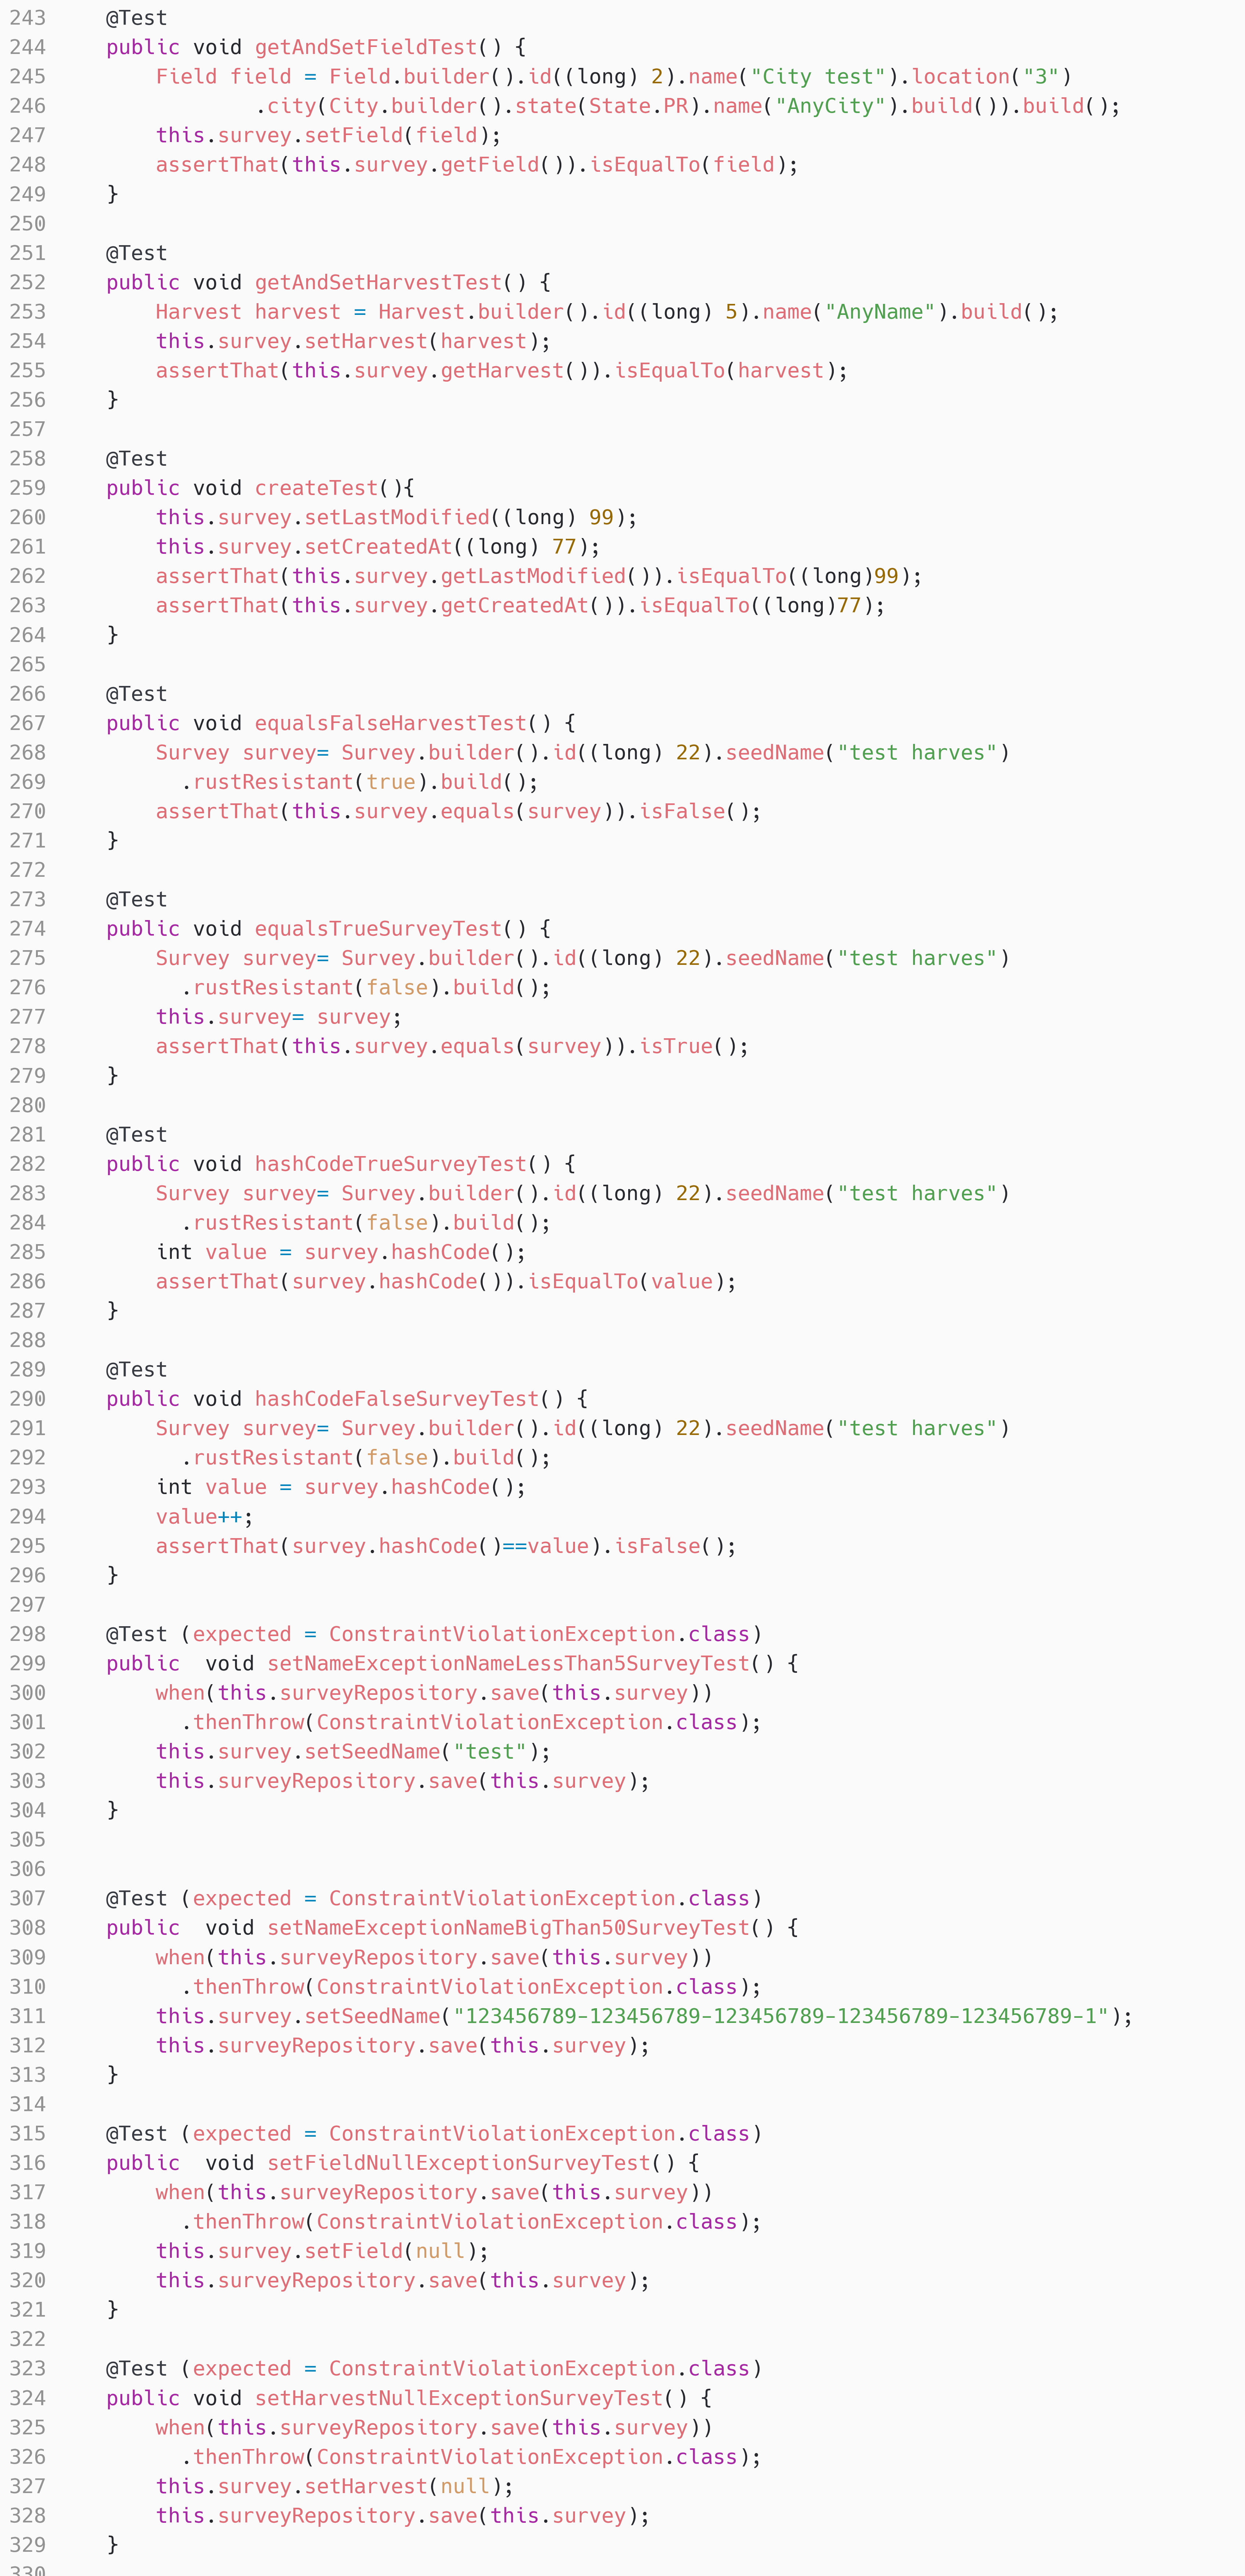
\includegraphics[scale=0.13]{dados/figuras/surveyTest3.png}
	\caption{Classe de Teste SurveyTest.java.}
	\label{testSurvey}
\end{figure}

Método de teste\textit{ “isRustResistantTest()”} linhas 34 a 40 figura \ref{testSurvey}:  Este método de teste consiste em recuperar o valor atribuído a variável\textit{ “rustResistant”} do objeto \textit{“Survey”.} A entrada é um \textit{“boolean”}(verdadeiro ou falso), a saída também se trata de um \textit{“boolean”}. A primeira assertiva recupera o valor atribuído na linha 25, \textit{“FALSE”}, e a saída do meto testado é um\textit{ “FALSE”}, linha 36, em seguida é atribuído a variável o valor \textit{“TRUE”}, linha 37 e 38, uma nova assertiva é feita e o valor recuperado é um \textit{“TRUE”}, linha 39.

Método de teste \textit{“isBtTest ()”} linhas 42 a 47 figura \ref{testSurvey}: Este método de teste consiste em recuperar o valor atribuído a variável\textit{ “bt”} do objeto \textit{“Survey”}. A entrada e um \textit{“boolean”}(verdadeiro ou falso), a saída também se trata de um \textit{“boolean”}. A primeira assertiva recupera o valor atribuído na linha 23, \textit{“FALSE”}, e a saída do meto testado é um \textit{“FALSE”}, linha 44, em seguida é atribuída a variável o valor \textit{“TRUE”}, linha 45 e 46, uma nova assertiva é feita e o valor recuperado é um \textit{“TRUE”}, linha 46.

Método de teste \textit{“getSowedDateTest()”} linhas 49 a 53 figura \ref{testSurvey}: Este teste consiste em recuperar a data atribuída a variável “\textit{“SowedDate”}” do objeto \textit{“Survey”}. A entrada é um objeto do tipo “\textit{“Date”}” que contém o valor de uma data com dia, mês e ano. A saída é um objeto do tipo “\textit{“Date”}” que contem o valor de uma data válida. A entrada é definida na linha 26, um outro objeto do tipo \textit{“Date”} é criado para comparação na linha 51. A assertiva é feita na linha 52 e compara o valor recuperado do meto testado com o valor definido na linha 51, os valores são iguais.  

Método de teste \textit{“getEmergenceDateTest()”} linhas 55 a 59 figura \ref{testSurvey}: Este teste consiste em recuperar a data atribuída a variável \textit{“EmergenceDate”} do objeto \textit{“Survey”}. A entrada é um objeto do tipo \textit{“Date”} que contém o valor de uma data com dia, mês e ano. A saída é um objeto do tipo \textit{“Date”} que contém o valor de uma data válida. A entrada é definida na linha 27, um outro objeto do tipo \textit{“Date”} é criado para comparação na linha 57. A assertiva é feita na linha 58 e compara o valor recuperado do meto testado com o valor definido na linha 57, os valores são iguais.  

Método de teste \textit{“getHarvestDateTest()”} linhas 61 a 65 figura \ref{testSurvey}: Este teste consiste em recuperar a data atribuída a variável \textit{“HarvestDate”} do objeto \textit{“Survey”}. A entrada é um objeto do tipo \textit{“Date”} que contém o valor de uma data com dia, mês e ano. A saída é um objeto do tipo \textit{“Date”} que contém o valor de uma data válida. A entrada é definida na linha 27, um outro objeto do tipo \textit{“Date”} é criado para comparação na linha 63. A assertiva é feita na linha 64 e compara o valor recuperado do meto testado com o valor definido na linha 63, os valores são iguais.  

Método de teste \textit{“getLongitudeTest()”} linhas 67 a 71 figura \ref{testSurvey}: Este teste consiste em recuperar o valor atribuído a variável \textit{“Longitude” }do objeto \textit{“LocationData”}  presente em uma pesquisa. A entrada consiste em um valor numérico de ponto flutuante \textit{“Double”} e a saída também consiste em um valor numérico do tipo \textit{“Double”}. A entrada é realizada na linha 24, o método é testado na linha 69, o retorno é o mesmo valor atribuído na linha 24.   

Método de teste \textit{“getLatitudeTest()”} linhas 72 a 75 figura \ref{testSurvey}: Este teste consiste em recuperar o valor atribuído a variável\textit{ “Latitude”} do objeto \textit{“LocationData”} presente em uma pesquisa. A entrada consiste em um valor numérico de ponto flutuante \textit{“Double”} e a saída também consiste em um valor numérico do tipo \textit{“Double”}. A entrada é realizada na linha 24, o método é testado na linha 74, o retorno é o mesmo valor atribuído na linha 24.

Método de teste \textit{“getProductivityFieldTest()”} linhas 77 a 80 figura \ref{testSurvey}: Este teste consiste em recuperar o valor atribuído a variável “productivityField” do objeto \textit{“ProductivityData”} presente em uma pesquisa. A entrada consiste em um valor numérico de ponto flutuante \textit{“Double”} e a saída também consiste em um valor numérico do tipo \textit{“Double”}. A entrada é realizada na linha 24, o método é testado na linha 74, o retorno é o mesmo valor atribuído na linha 24.

Método de teste \textit{“getProductivityFarmerTest()”} linhas 82 a 85 figura \ref{testSurvey}: Este teste consiste em recuperar o valor atribuído a variável\textit{ “productivityFarmer”} do objeto \textit{“ProductivityData”} presente em uma pesquisa. A entrada consiste em um valor numérico de ponto flutuante \textit{“Double”} e a saída também consiste em um valor numérico do tipo \textit{“Double”}. A entrada é realizada na linha 24, o método é testado na linha 79, o retorno é o mesmo valor atribuído na linha 24.

Método de teste \textit{“isSeparatedWeightTest()”} linhas 87 a 93 figura \ref{testSurvey}: Este método de teste consiste em recuperar o valor atribuído a variável\textit{ “SeparatedWeight”} do objeto \textit{“ProductivityData”} presente em uma pesquisa. A entrada e um \textit{“boolean”}(verdadeiro ou falso), a saída também se trata de um \textit{“boolean”}. A primeira assertiva recupera o valor atribuído na linha 25, \textit{“FALSE”}, e a saída do meto testado é um \textit{“FALSE”}, linha 44, em seguida é atribuída a variável o valor \textit{“TRUE”}, linha 90 e 91, uma nova assertiva é feita é o valor recuperado é um \textit{“TRUE”}, linha 92.

Método de teste \textit{“getTotalAreaTest()”} linhas 95 a 98 figura \ref{testSurvey}: Este teste consiste em recuperar o valor atribuído a variável\textit{ “TotalArea”} do objeto \textit{“SizeData”} presente em uma pesquisa. A entrada consiste em um valor numérico de ponto flutuante \textit{“Double”} e a saída também consiste em um valor numérico do tipo \textit{“Double”}. A entrada é realizada na linha 25, o método é testado na linha 97, o retorno é o mesmo valor atribuído na linha 25.

Método de teste \textit{“getTotalPlantedAreaTest()”} linhas 100 a 103 figura \ref{testSurvey}: Este teste consiste em recuperar o valor atribuído a variável \textit{“TotalPlantedArea”} do objeto \textit{“SizeData”} presente em uma pesquisa. A entrada consiste em um valor numérico de ponto flutuante \textit{“Double”} e a saída também consiste em um valor numérico do tipo \textit{“Double”}. A entrada é realizada na linha 26, o método é testado na linha 102, o retorno é o mesmo valor atribuído na linha 26.

Método de teste \textit{“getPlantPerMeterTest()”} linhas 105 a 108 figura \ref{testSurvey}: Este teste consiste em recuperar o valor atribuído a variável\textit{ “plantPerMeter”} do objeto \textit{“SizeData”} presente em uma pesquisa. A entrada consiste em um valor numérico de ponto flutuante \textit{“Double”} e a saída também consiste em um valor numérico do tipo \textit{“Double”}. A entrada é realizada na linha 24, o método é testado na linha 107, o retorno é o mesmo valor atribuído na linha 24.

Método de teste \textit{“getFieldIdTest()”} linhas 110 a 113 figura \ref{testSurvey}: Este teste consiste em recuperar o identificador único de um objeto \textit{“Field”} presente em uma pesquisa. A entrada consiste em um objeto do tipo \textit{“Field”} que possui um identificador único, a saída é o identificador único, um valor numérico do tipo \textit{“Long”}. A entrada é feita nas linhas 27 e 28, a assertiva é feia na linha 112, o valor recuperado é o mesmo atribuído na linha 27.

Método de teste\textit{ “getFieldNameTest()”} linhas 115 a 118 figura \ref{testSurvey}: Este teste consiste em recuperar o nome atribuído a um objeto \textit{“Field”} presente em uma pesquisa. A entrada consiste em um objeto do tipo \textit{“Field”} que possui um nome, a saída é o nome contido no objeto, uma \textit{String”} de caracteres normalizados com o primeiro caractere de cada conjunto de caracteres maiúsculo. A entrada é feita nas linhas 27 e 28, a assertiva é feia na linha 117, o valor recuperado é o mesmo atribuído na linha 27 mais com o primeiro caractere de cada conjunto maiúsculo.

Método de teste \textit{“getFieldLocationTest()”} linhas 120 a 123 figura \ref{testSurvey}: Este teste consiste em recuperar a localização atribuída a um objeto \textit{“Field”} presente em uma pesquisa. A entrada consiste em um objeto do tipo \textit{“Field”} que possui uma localização, a saída é a localização contida no objeto, uma \textit{“String”} de caracteres. A entrada é feita nas linhas 27 e 28, a assertiva é feia na linha 122, o valor recuperado é o mesmo atribuído na linha 27.

Método de teste\textit{ “getFieldCityIdTest()”} linhas 125 a 128 figura \ref{testSurvey}: Este teste consiste em recuperar o identificador único de um objeto \textit{“City”} presente em uma pesquisa. A entrada consiste em um objeto do tipo \textit{“Field”} que possui uma cidade com identificador único, a saída é o identificador do único da cidade, um valor numérico do tipo \textit{“Long”}. O objeto \textit{“City”} é criado nas linhas 16 e 17, a entrada é feita nas linhas 27 e 28, a assertiva é feia na linha 127, o valor recuperado é o mesmo atribuído na linha 17.


Método de teste \textit{“getFieldCityNameTest()”} linhas 130 a 133 figura \ref{testSurvey}: Este teste consiste em recuperar o nome de um objeto \textit{“City”} presente em uma pesquisa. A entrada consiste em um objeto do tipo \textit{“Field”} que possui uma cidade com um nome, a saída é uma \textit{“String”} de caracteres normalizados com o primeiro caractere de cada conjunto maiúsculo. O objeto \textit{“City”} é criado nas linhas 16, a entrada é feita nas linhas 27 e 28, a assertiva é feia na linha 132, o valor recuperado é o mesmo atribuído na linha 16 mais com o primeiro caractere de cada conjunto maiúsculo.

Método de teste \textit{“getFieldCityStateTest()”} linhas 135 a 138 figura \ref{testSurvey}: Este teste consiste em recuperar o estado de um objeto \textit{“City”} presente em uma pesquisa. A entrada consiste em um objeto do tipo \textit{“Field”} que possui uma cidade com um estado, a saída é um objeto do tipo \textit{“State.PR”}. O objeto \textit{“City”} é criado nas linhas 16, a entrada é feita nas linhas 27 e 28, a assertiva é feia na linha 137, o valor recuperado é o mesmo atribuído na linha 16.

Método de teste \textit{“getFarmerIdTest()”} linhas 140 a 143 figura \ref{testSurvey}: Este teste consiste em recuperar o identificador único de um objeto \textit{“Farmer”} presente em uma pesquisa. A entrada consiste em um objeto do tipo \textit{“Field”} que possui um agricultor com identificador único, a saída é o identificador do único do agricultor, um valor numérico do tipo \textit{“Long”}. O objeto \textit{“Farmer”} é criado na linha 29, a entrada é feita na linha 27, 28 e 29, a assertiva é feia na linha 142, o valor recuperado é o mesmo atribuído na linha 29.

Método de teste \textit{“getFarmerStringTest()”} linhas 145 a 148 figura \ref{testSurvey}: Este teste consiste em recuperar o nome de um objeto \textit{“Farmer”} presente em uma pesquisa. A entrada consiste em um objeto do tipo \textit{“Field”} que possui um agricultor com um nome, a saída é uma \textit{“String”} de caracteres normalizados com o primeiro caractere de cada conjunto maiúsculo. O objeto \textit{“Farmer”} é criado nas linhas 29, a entrada é feita nas linhas 27, 28 e 29, a assertiva é feia na linha 147, o valor recuperado é o mesmo atribuído na linha 29 mais com o primeiro caractere de cada conjunto maiúsculo.

Método de teste \textit{“getFieldSupervisorsTest()”} linhas 150 a 155 figura \ref{testSurvey}: Este teste consiste em recuperar os supervisores presentes em um objeto \textit{“Field”} presente em uma pesquisa. A entrada consiste em um objeto do tipo \textit{“Field”} que possua um ou mais supervisores, a saída é uma lista de objetos do tipo \textit{“Supervisor”} que contem os supervisores presentes no \textit{“Field”} presente na pesquisa. Uma lista de supervisores é criada nas linhas 12 a 15, a entrada é feita nas linhas 27, 28 e 29, a assertiva é feia nas linhas 152 e 153, o valor recuperado e uma lista de supervisores que contem os supervisores declarados nas linhas 5, 6 e 7.


Método de teste \textit{“getHarvestIdTest()”} linhas 157 a 160 figura \ref{testSurvey}: Este teste consiste em recuperar o identificador único de um objeto \textit{“Harvest”} presente em uma pesquisa. A entrada consiste em um objeto do tipo \textit{“Harvest”} que possui um identificador único, a saída é o identificador do único da colheita, um valor numérico do tipo \textit{“Long”}. O objeto \textit{“Harvest”} é criado na linha 30, a entrada é feita nas linhas 27, 28, 29 e 30 a assertiva é feia na linha 159, o valor recuperado é o mesmo atribuído na linha 30.

Método de teste \textit{“getHarvestNameTest()”} linhas 162 a 165 figura \ref{testSurvey}: Este teste consiste em recuperar o nome de um objeto \textit{“Harvest”} presente em uma pesquisa. A entrada consiste em um objeto do tipo \textit{“Harvest”} que possui um nome, a saída é uma \textit{“String”} de caracteres normalizados com o primeiro caractere de cada conjunto maiúsculo. O objeto \textit{“Harvest”} é criado nas linhas 30, a entrada é feita nas linhas 27, 28, 29 e 30, a assertiva é feia na linha 164, o valor recuperado é o mesmo atribuído na linha 30 mais com o primeiro caractere de cada conjunto maiúsculo.

Método de teste \textit{“getHarvestBeginDateTest()”} linhas 167 a 171 figura \ref{testSurvey}: Este teste consiste em recuperar a data da variável \textit{“BeginDate”} atribuída a um objeto \textit{“Harvest”} presente em uma pesquisa. A entrada é um objeto do tipo \textit{“Harvest”} que possui um \textit{“Date”} que contém o valor de uma data com dia, mês e ano. A saída é um objeto do tipo \textit{“Date”} que contém o valor de uma data válida. A entrada é definida na linha 30, um outro objeto do tipo \textit{“Date”} é criado para comparação na linha 169. A assertiva é feita na linha 170 e compara o valor recuperado do meto testado com o valor definido na linha 169, os valores são iguais.  

Método de teste \textit{“getHarvestEndDateTest()”} linhas 173 a 177 figura \ref{testSurvey}: Este teste consiste em recuperar a data da variável \textit{“EndDate” }atribuída a um objeto \textit{“Harvest”} presente em uma pesquisa. A entrada é um objeto do tipo \textit{“Harvest”} que possui um \textit{“Date”} que contém o valor de uma data com dia, mês e ano. A saída é um objeto do tipo \textit{“Date”} que contém o valor de uma data válida. A entrada é definida na linha 30, um outro objeto do tipo \textit{“Date”} é criado para comparação na linha 175. A assertiva é feita na linha 176 e compara o valor recuperado do meto testado com o valor definido na linha 175, os valores são iguais.  

Método de teste \textit{“getFieldSupervisorNamesTest()”} linhas 179 a 182 figura \ref{testSurvey}: Este teste consiste em recuperar os nomes dos supervisores presentes em um objeto \textit{“Field”} presente em uma pesquisa. A entrada consiste em um objeto do tipo \textit{“Field”} que possua um ou mais supervisores, a saída é uma \textit{“String”} que contém os nomes dos supervisores presentes no objeto \textit{“Field”} presente na pesquisa. Uma lista de supervisores é criada nas linhas 12 a 15, a entrada é feita nas linhas 27, 28 e 29, a assertiva é feia nas linhas 181, o valor recuperado e uma \textit{“String”} com o nome dos supervisores declarados nas linhas 5, 6 e 7.

Método de teste \textit{“getAndSetIdTest()”} linhas 184 a 188 figura \ref{testSurvey}: Este teste consiste em atribuir e recuperar o identificador único de uma pesquisa. A entrada consiste em um valor numérico do tipo \textit{“Long”}, a saída é um valor numérico do tipo \textit{“Long”}. A entrada e feita na linha 186, a saída e feita na assertiva linha 187, que compara a saída com o valor atribuído, os valores são iguais.

Método de teste \textit{“getAndSeedNameTest()”} linhas 190 a 194 figura \ref{testSurvey}: Este teste trata de atribuir um valor da variável \textit{“Seed”} do tipo \textit{“String”} do objeto \textit{“Survey”}. A entrada consiste em uma \textit{“String”} de caracteres, a saída é uma string de caracteres normalizada. A assertiva é feita na linha 193 e o valor recuperado é idêntico ao atribuído, mas com a primeira letra de cada conjunto de caracteres maiúscula.

Método de teste \textit{“isSporeCollectorPresentTest()”} linhas 196 a 202 figura \ref{testSurvey}: Este método de teste consiste em recuperar o valor atribuído a variável \textit{“SporeCollectorPresent” }do objeto \textit{“Survey”}. A entrada e um \textit{“boolean”}(verdadeiro ou falso), a saída também se trata de um \textit{“boolean”}. A primeira assertiva recupera o valor atribuído na linha 198, \textit{“FALSE”}, e a saída do meto testado é um \textit{“FALSE”}, linha 199, em seguida é atribuída a variável o valor \textit{“TRUE”}, linha 200, uma nova assertiva é feita é o valor recuperado é um \textit{“TRUE”}, linha 201.

Método de teste \textit{“getAndSetQuestionDataTest()”} linhas 204 a 209 figura \ref{testSurvey}: Este teste trata de atribuir um objeto do tipo \textit{“QuestionData” }a \textit{“Survey”} em seguida faz a recuperação do mesmo. A entrada é um objeto do tipo \textit{“QuestionData”,} a saída é um objeto do tipo\textit{ “QuestionData”}. A entrada é feita na linha 207, a saída é feita a linha 208 juntamente da assertiva que compara o objeto recuperado com o objeto inserido, os dois são iguais.

Método de teste \textit{“getAndSetDateDataTest()”} linhas 211 a 218 figura \ref{testSurvey}: Este teste trata de atribuir um objeto do tipo \textit{“DateData”} a \textit{“Survey”} em seguida faz a recuperação do mesmo. A entrada é um objeto do tipo “DateData”, a saída é um objeto do tipo \textit{“DateData”}. A entrada é feita na linha 216, a saída é feita a linha 217 juntamente da assertiva que compara o objeto recuperado com o objeto inserido, os dois são iguais.

Método de teste \textit{“getSizeDataTest()”} linhas 220 a 225 figura \ref{testSurvey}: Este teste trata de atribuir um objeto do tipo \textit{“SizeData”} a \textit{“Survey”} em seguida faz a recuperação do mesmo. A entrada é um objeto do tipo “SizeData”, a saída é um objeto do tipo \textit{“SizeData”}. A entrada é feita na linha 223, a saída é feita a linha 224 juntamente da assertiva que compara o objeto recuperado com o objeto inserido, os dois são iguais.

Método de teste \textit{“getLocationDataTest()”} linhas 227 a 233 figura \ref{testSurvey}: Este teste trata de atribuir um objeto do tipo \textit{“LocationData”} a \textit{“Survey”} em seguida faz a recuperação do mesmo. A entrada é um objeto do tipo \textit{“LocationData”}, a saída é um objeto do tipo \textit{“LocationData”}. A entrada é feita na linha 231, a saída é feita a linha 232 juntamente da assertiva que compara o objeto recuperado com o objeto inserido, os dois são iguais.

Método de teste \textit{“getAndSetProductivityDataTest()”} linhas 235 a 241 figura \ref{testSurvey}: Este teste trata de atribuir um objeto do tipo \textit{“ProductivityData” }a \textit{“Survey”} em seguida faz a recuperação do mesmo. A entrada é um objeto do tipo \textit{“ProductivityData”}, a saída é um objeto do tipo “ProductivityData”. A entrada é feita na linha 239, a saída é feita a linha 240 juntamente da assertiva que compara o objeto recuperado com o objeto inserido, os dois são iguais.

Método de teste \textit{“getAndSetFieldTest()”} linhas 243 a 249 figura \ref{testSurvey}: Este teste trata de atribuir um objeto do tipo \textit{“Field”} a \textit{“Survey”} em seguida faz a recuperação do mesmo. A entrada é um objeto do tipo \textit{“Field”}, a saída é um objeto do tipo \textit{“Field”}. A entrada é feita na linha 247, a saída é feita a linha 248 juntamente da assertiva que compara o objeto recuperado com o objeto inserido, os dois são iguais.

Método de teste \textit{“getAndSetHarvestTest()”} linhas 251 a 256 figura \ref{testSurvey}: Este teste trata de atribuir um objeto do tipo \textit{“Harvest”} a \textit{“Survey”} em seguida faz a recuperação do mesmo. A entrada é um objeto do tipo \textit{“Harvest”}, a saída é um objeto do tipo \textit{“Harvest”}. A entrada é feita na linha 254, a saída é feita a linha 255 juntamente da assertiva que compara o objeto recuperado com o objeto inserido, os dois são iguais.

Método de teste \textit{“createTest()”} linhas 258 a 264 figura \ref{testSurvey}: Este método é responsável por testar os atributos criados na superclasse \textit{“auditingPersistenceEntity”,} como uma superclasse não pode ser testada os métodos e atributos dela devem ser testados em uma das suas subclasses.  A classe e composta por dois atributos do tipo long \textit{“LastModified” }e \textit{“CreatedAt”}, O objetivo deste teste é de atribuir valor as variáveis e verificar se os valores atribuídos são recuperados corretamente. As entradas foram criadas nas linhas 260 e 261 respectivamente. Posteriormente nas linhas 262 e 263 e feita a confirmação das saídas contendo os valores 99 e 77 do tipo \textit{“Long”}.

Método de teste \textit{“equalsFalseHarvestTest()”} linhas 266 a 272 figura \ref{testSurvey}: Este método de teste consiste em comparar dois objetos do tipo \textit{“Survey”} caso eles sejam iguais o retorno é um \textit{“boolean”} \textit{“TRUE”} caso sejam diferentes o retorno é um \textit{“FALSE”}. A entrada consiste em dois objetos do tipo \textit{“Survey”}, o primeiro objeto é criado nas linhas 26, 27, 28 e 29, o segundo objeto é criado nas linhas 268 e 269. A saída é um \textit{“FALSE”} pois os objetos comparados são diferentes.

Método de teste \textit{“equalsTrueSurveyTest()”} linhas 273 a 279 figura \ref{testSurvey}: Este método de teste consiste em comparar dois objetos do tipo \textit{“Survey”} caso eles sejam iguais o retorno é um \textit{“boolean”} \textit{“TRUE”} caso sejam diferentes o retorno é um \textit{“FALSE”}. A entrada consiste em dois objetos do tipo \textit{“Survey”}, o primeiro objeto é criado nas linhas 26, 27, 28 e 29, o segundo objeto é criado nas linhas 275 e 276, o primeiro objeto recebe uma cópia do segundo objeto. A saída é um \textit{“TRUE”} pois os objetos são iguais.

Método de teste \textit{“hashCodeTrueSurveyTest()”} linhas 281 a 287 figura \ref{testSurvey}: Este teste consiste em recuperar o valor de \textit{“hashcode”} de um objeto e verifica seu valor em uma segunda chamada. O método não possui entrada. A saída consiste em um valor numérico do tipo \textit{“int”.} O valor de hash é recuperado em uma primeira chamada na linha 285, em seguida é feita uma assertiva, esta compara o valor recuperado anteriormente com o valor de uma nova chamda do método de hash, os valores são iguais.

Método de teste\textit{ “hashCodeFalseSurveyTest()”} linhas 289 a 296 figura \ref{testSurvey}: Este teste consiste em recuperar o valor de \textit{“hashcode”} de um objeto e verifica seu valor em uma segunda chamada. O método não possui entrada. A saída consiste em um valor numérico do tipo\textit{ “int”}. O valor é de hash é recuperado em uma primeira chamada na linha 293, em seguida é feito um incremento no valor recuperado. Uma assertiva compara o valor chamado incrementado com o valor de uma nova chamda do método de hash, os valores são diferentes.


Método de teste \textit{“setNameExceptionNameLessThan5SurveyTest()”} linhas 298 a 304 figura \ref{testSurvey}: Uma das restrições que se encontra na hora de salvar um objeto do tipo \textit{“Survey”} é que a variável “Seed” do tipo \textit{“String”} deve ter entre 5 e 50 caracteres. A entrada consiste em uma \textit{“String”} contendo apenas quatro caractere. A saída esperada é uma exceção de violação das regras do banco. A saída deste teste é uma \textit{“ConstraintViolationException.class”} disparada pelo \textit{“SurveyRepository.class”} pois o valor atribuído é menor que a regra estipulado.

Método de teste “setNameExceptionNameBigThan50SurveyTest()” linhas 307 a 313 figura \ref{testSurvey}: Uma das restrições que se encontra na hora de salvar um objeto do tipo \textit{“Survey”} é que a variável “Seed” do tipo \textit{“String”} deve ter entre 5 e 50 caracteres. A entrada consiste em uma \textit{“String”} contendo apenas cinquenta e um caractere. A saída esperada é uma exceção de violação das regras do banco. A saída deste teste é uma \textit{“ConstraintViolationException.class”} disparada pelo \textit{“SurveyRepository.class” }pois o valor atribuído é maior que a regra estipulado.

Método de teste \textit{“setFieldNullExceptionSurveyTest()”} linhas 315 a 321 figura \ref{testSurvey}: Uma das restrições que se encontra na hora de salvar um objeto do tipo \textit{“Survey”} é que a pesquisa deve possuir um objeto do tipo \textit{“Field”}. A entrada consiste em uma \textit{“null”.} A saída esperada é uma exceção de violação das regras do banco. A saída deste teste é uma \textit{“ConstraintViolationException.class”} disparada pelo \textit{“SurveyRepository.class”} pois o objeto atribuído é nulo.

Método de teste \textit{“setHarvestNullExceptionSurveyTest()”} linhas 323 a 329 figura \ref{testSurvey}: Uma das restrições que se encontra na hora de salvar um objeto do tipo \textit{“Survey”} é que a pesquisa deve possuir um objeto do tipo \textit{“Field”}. A entrada consiste em uma \textit{“null”}. A saída esperada é uma exceção de violação das regras do banco. A saída deste teste é uma\textit{ “ConstraintViolationException.class” }disparada pelo \textit{“SurveyRepository.class” }pois o objeto atribuído é nulo.



Após a execução dos testes a cobertura das entradas e saídas de dados da classe \textit{Survey.java} é de 100\%. 


\section{RESULTADO GERAL DOS TESTES PACOTE ENTITY}

Para alcançar a cobertura de 100\%  de todos os métodos linhas e classes do pacote\textit{Entity}foram criados no total 358 testes de unidade, onde 357 foram aprovados e 1 rejeitado. Cada classe possui o seguinte número de casos de teste: 

\begin{itemize}
        \item Pacote Base:
\begin{itemize}
    \item Classe \textit{FieldTest}: 20 casos de teste aprovados, 1 reprovado;
    \item Classe \textit{RegionTest}: 18 casos de teste aprovados;
    \item Classe \textit{FarmerTest}: 5 casos de teste aprovados;
    \item Classe \textit{StateTest}: 1 casos de teste aprovados;
    \item Classe \textit{MacroRegionTest}: 8 casos de teste aprovados;
    \item Classe \textit{CityTest}: 5 casos de teste aprovados;
    \item Classe \textit{SupervisorTest}: 13 casos de teste aprovados;
\end{itemize}
  \item Pacote MIP:
  \begin{itemize} 
    \item Classe \textit{GrowthPhaseTest}: 1 casos de teste aprovados;
    \item Classe \textit{PestDiseaseTest}: 9 casos de teste aprovados;
    \item Classe \textit{PestNaturalPredatorTest}: 9 casos de teste aprovados;
    \item Classe \textit{PestSizeTest}: 1 casos de teste aprovados;
    \item Classe \textit{PestTest}: 12 casos de teste aprovados;
    \item Classe \textit{MIPSampleNaturalPredatorOccurrenceTest}: 8 casos de teste aprovados;
    \item Classe \textit{MIPSamplePestDiseaseOccurrenceTest}: 8 casos de teste aprovados;
    \item Classe \textit{MIPSamplePestOccurrenceTest}: 10 casos de teste aprovados;
    \item Classe \textit{MIPSampleTest}: 23 casos de teste aprovados;
\end{itemize}
  \item Pacote \textit{Survey}:
  \begin{itemize}   
    \item Classe \textit{SurveyTest}: 8 casos de teste aprovados;46
    \item Classe \textit{HarvestTest}: 11 casos de teste aprovados;
    \item Classe \textit{DateDataTest}: 3 casos de teste aprovados;
    \item Classe \textit{LocationDataTest}: 7 casos de teste aprovados;
    \item Classe \textit{ProductivityDataTest}: 8 casos de teste aprovados;
    \item Classe \textit{QuestionDataTest}: 7 casos de teste aprovados;
    \item Classe \textit{SizeDataTest}: 4 casos de teste aprovados;
\end{itemize}
  \item Pacote MID:
  \begin{itemize}
    \item Classe \textit{BladeReadingResponsibleEntityTest}: 7 casos de teste aprovados;
    \item Classe \textit{AsiaticRustTypesLeafInspectionTest}: 1 casos de teste aprovados;
    \item Classe \textit{AsiaticRustTypesSporeCollectorTest}: 1 casos de teste aprovados;
    \item Classe \textit{MIDSampleFungicideApplicationOccurrenceTest}: 9 casos de teste aprovados;
    \item Classe \textit{MIDSampleLeafInspectionOccurrenceTest}: 7 casos de teste aprovados;
    \item Classe \textit{MIDSampleSporeCollectorOccurrenceTest}: 9 casos de teste aprovados;
    \item Classe \textit{MIDRustSampleTest}: 12 casos de teste aprovados;
    \item Classe \textit{BladeReadingResponsiblePersonTest}: 8 casos de teste aprovados;
    \end{itemize}
    \item Pacote \textit{Pulverisation}:
  \begin{itemize}
    \item Classe \textit{ProductTest}: 16 casos de teste aprovados;
    \item Classe \textit{ProductUnitTest}: 1 casos de teste aprovados;
    \item Classe \textit{PulverisationOperationOccurrenceTest}: 13 casos de teste aprovados;
    \item Classe \textit{PulverisationOperationTest}: 23 casos de teste aprovados;
    \item Classe \textit{TargetCategoryTest}: 1 casos de teste aprovados;
    \item Classe \textit{TargetTest}: 11 casos de teste aprovados;
    \end{itemize}
    \end{itemize}



Como já dito anterior mente os testes não podem garantir que o software é livre de defeitos mas, seu objetivo principal é revelar a presença de defeitos. Após a execução dos testes a taxa de cobertura foi de: 100\% das classes, 100\% dos métodos e 100\% das linhas.


\section{APURAÇÃO DOS TESTES PACOTE SERVICE}



O pacote \textit{service} é responsável por armazenar as classes que realizam o fluxo de dados entre  os repositórios e entidades com as demais camadas superiores da arquitetura (camada de apresentação, \textit{web}, \textit{controle}), além de implementar regras de negócios especificas que não cabem as camadas inferiores, o que possibilita o consumo dos dados a diferentes tipos de serviços sem que este serviços que consumirão os dados necessitem implementar novamente as regras de negócio evitando a duplicação de código. O pacote é composto por 5 sub pacotes sendo eles: 


\begin{itemize}

\item[1] Pacote base: Armazenas as classes que realiza a comunicação com as entidades e repositórios do pacote \textit{Entity}/base. Operações como leitura de dados, escrita de dados, atualização de dados e exclusão de dados são responsabilidades destas classes. As classes contidas neste pacote são: \textit{CityService.java, FarmerService.java, SupervisorService.java, RegionService.java, MacroRegionService.java, LocalDateTimeConverter e FieldService.java};  

\item[2] Pacote mid: Armazenas as classes que realiza a comunicação com as entidades e repositórios do pacote \textit{Entity}/mid. Operações como leitura de dados, escrita de dados, atualização de dados e exclusão de dados são responsabilidades destas classes. As classes contidas neste pacote são: \textit{BladeReadingResponsibleEntityService.java, BladeReadingResponsiblePersonService.java e MIDRustSampleService.java};

\item[3] Pacote mip: Armazenas as classes que realiza a comunicação com as entidades e repositórios do pacote\textit{Entity}/mip. Operações como leitura de dados, escrita de dados, atualização de dados e exclusão de dados são responsabilidades destas classes. As classes contidas neste pacote são: \textit{MIPSampleService.java, PestDiseaseService.java, PestNaturalPredatorService.java e PestService.java;}

\item[4] Pacote \textit{pulverisation}: Armazenas as classes que realiza a comunicação com as entidades e repositórios do pacote\textit{Entity}/pulverisation. Operações como leitura de dados, escrita de dados, atualização de dados e exclusão de dados são responsabilidades destas classes. As classes contidas neste pacote são: \textit{ProductService.java, PulverisationOperationService.java e TargetService.java;}

\item[5] Pacote \textit{survey}: Armazenas as classes que realiza a comunicação com as entidades e repositórios do pacote\textit{Entity}/survey. Operações como leitura de dados, escrita de dados, atualização de dados e exclusão de dados são responsabilidades destas classes. As classes contidas neste pacote são: \textit{HarvestService.java e SurveyService.java};

\end{itemize}

\subsection{RESULTADO DOS TESTES CLASSE FIELDSERVICE.JAVA}


\begin{figure}[H]
	\centering
	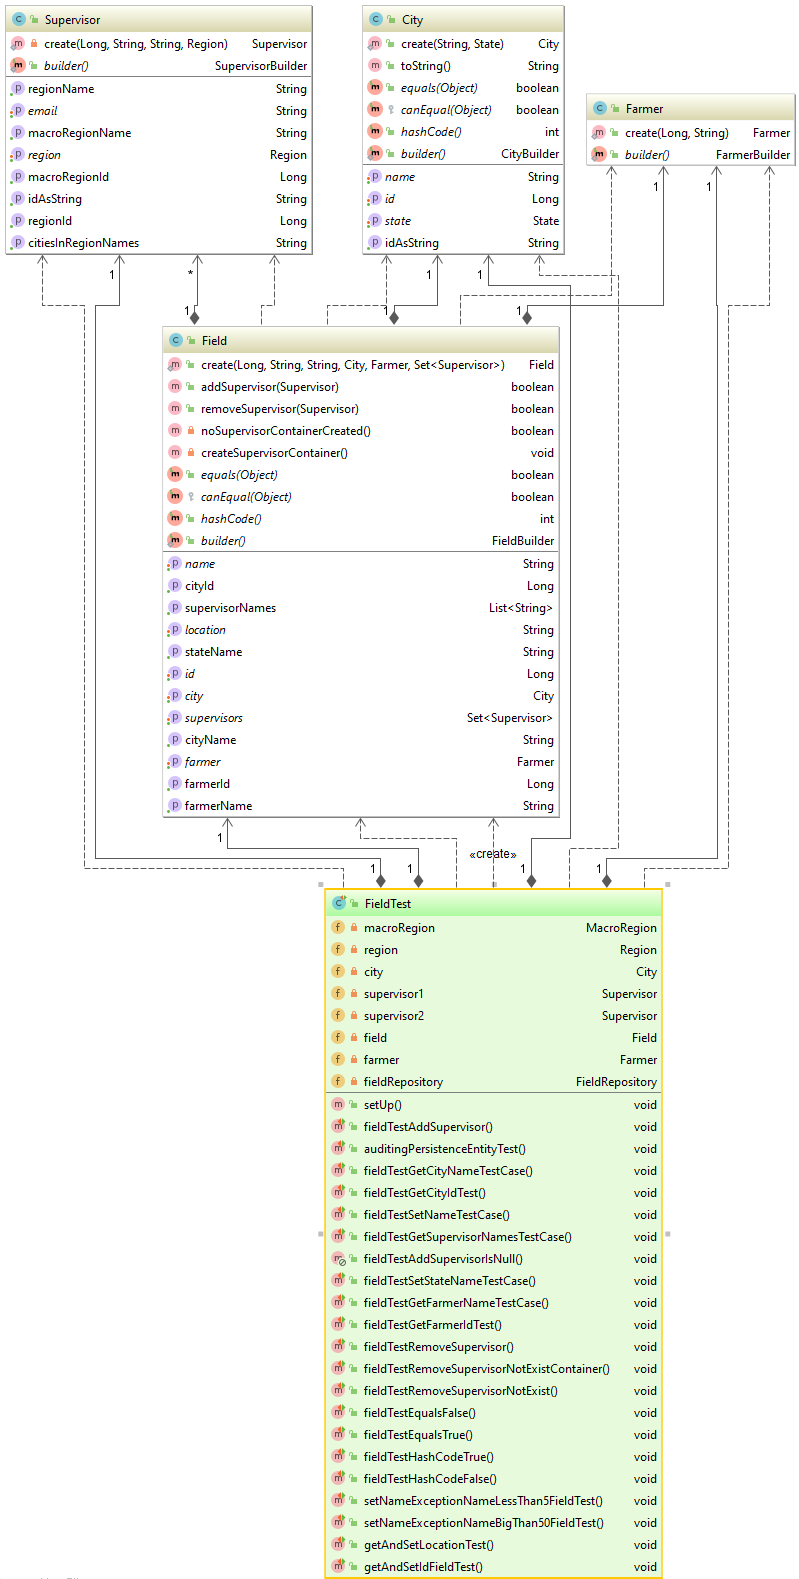
\includegraphics[scale=0.5]{dados/figuras/PackagebaseTestField.png}
	\caption{Diagrama de classes FieldServiceTest.java.}
	\label{packFieldService}
\end{figure}

A classe \textit{FieldService}é responsável por realizar a comunicação com a classe \textit{Field}, e com as demais classes que a compõem. A FIGURA \ref{packFieldService} apresenta o diagrama de classes da classe \textit{FieldService}e as demais classes que a compõem assim como a classe responsável por realizar os testes de seus métodos e variáveis. Também é possível analisar no diagrama os atributos e métodos que pertence à classe \textit{ FieldService }, assim como os métodos e atributos da classe de \textit{ FieldServiceTest}.  


A classe de teste apresentada na FIGURA \ref{packFieldService} possui vinte e três métodos de teste é um método de apoio aos testes denominado \textit{“setUp”}, o objetivo dos testes é exercitar a classe \textit{FieldService} até que todos as variáveis, entradas e saídas de dados sejam executados pelo menos uma vez. Como a classe \textit{FieldService} trabalha com outras classes além da \textit{Field} se faz necessário a instanciação destas como: \textit{Supervisor}, \textit{Farmer}, \textit{City} e outras para a execução completa dos testes. Como a classe trabalha com entidades que serão persistidas em um banco de dados, foi preciso criar uma referência para a interface \textit{FieldRepository} e outros repositórios que são chamados durante a execução dos testes. Como o objetivo deste trabalho é cobrir o sistema com testes unitários e testes que integram classes entidades com o banco de dados ou comunicação com APIs são testes de integração foi utilizado\textit{ “Mocks”} para simular o comportamento dos repositórios.



A FIGURA \ref{testeFieldService} apresenta a declaração da classe de teste, os atributos utilizados para desenvolver os testes e o método\textit{ “setUp”} utilizado para preparar o ambiente para os teste.

O trecho de código da FIGURA \ref{testeFieldService} apresenta as seguintes funcionalidades:

\begin{itemize}
\item Linha 1 A anotação \textit{@RunWith} permite a execução dos testes dentro de um contexto do \textit{Spring}. O comando \textit{SpringRunner}.class fornece suporte para carregar um \textit{Spring} \textit{ApplicationContext} e ter \textit{beans }\textit{@Autowired} na instância de teste.
\item Na linha 2 é utilizada a anotação \textit{@SpringBootTest} que prepara um contexto \textit{Spring} e inclui a possibilidade de iniciar um container em um porta default ou configurada pelo usuário. Neste caso a porta foi definida de forma randômica através do comando \textit{“SpringBootTest.WebEnvironment.RANDOM\_PORT”}; 

 \item Na linha 3 é utilizada a anotação \textit{@FixMethodOrder} que permite definir uma ordem de execução dos testes, neste casso foi definida a ordem \textit{“NAME\_ASCENDING"} que faz a execução dos testes de acordo com o nome de maneira ascendente;

 \item Linha 4 a classe \textit{FieldServiceTest} é aberta;

 \item Da linha 6 a 15 há a declaração dos objetos \textit{MOCKs} que serão utilizadas para a comunicação com o banco de dados. A anotação \textit{@MockBean} foi utilizada na declaração destas variáveis, ela permite que caso exista um \textit{bean }compatível com a classe declarada no contexto da aplicação \textit{Spring} este \textit{bean }será substituído por um \textit{Mock};

\item Linhas 14 e 15 uma instancia da classe \textit{FieldService}é declarada, a anotação \textit{@Autowired} é utilizada para a injeção automática de um \textit{bean }correspondente ao declarado na variável.
 
\item Da linha 17 a 21 há a declaração dos objetos que serão utilizados nos testes;

 



\item Na linha 24 é utilizado a anotação \textit{@Before}, esta anotação determina que sempre antes da execução de um teste o método \textit{“setUp”} deve ser executado primeiro.


\begin{figure}[H]
	\centering
	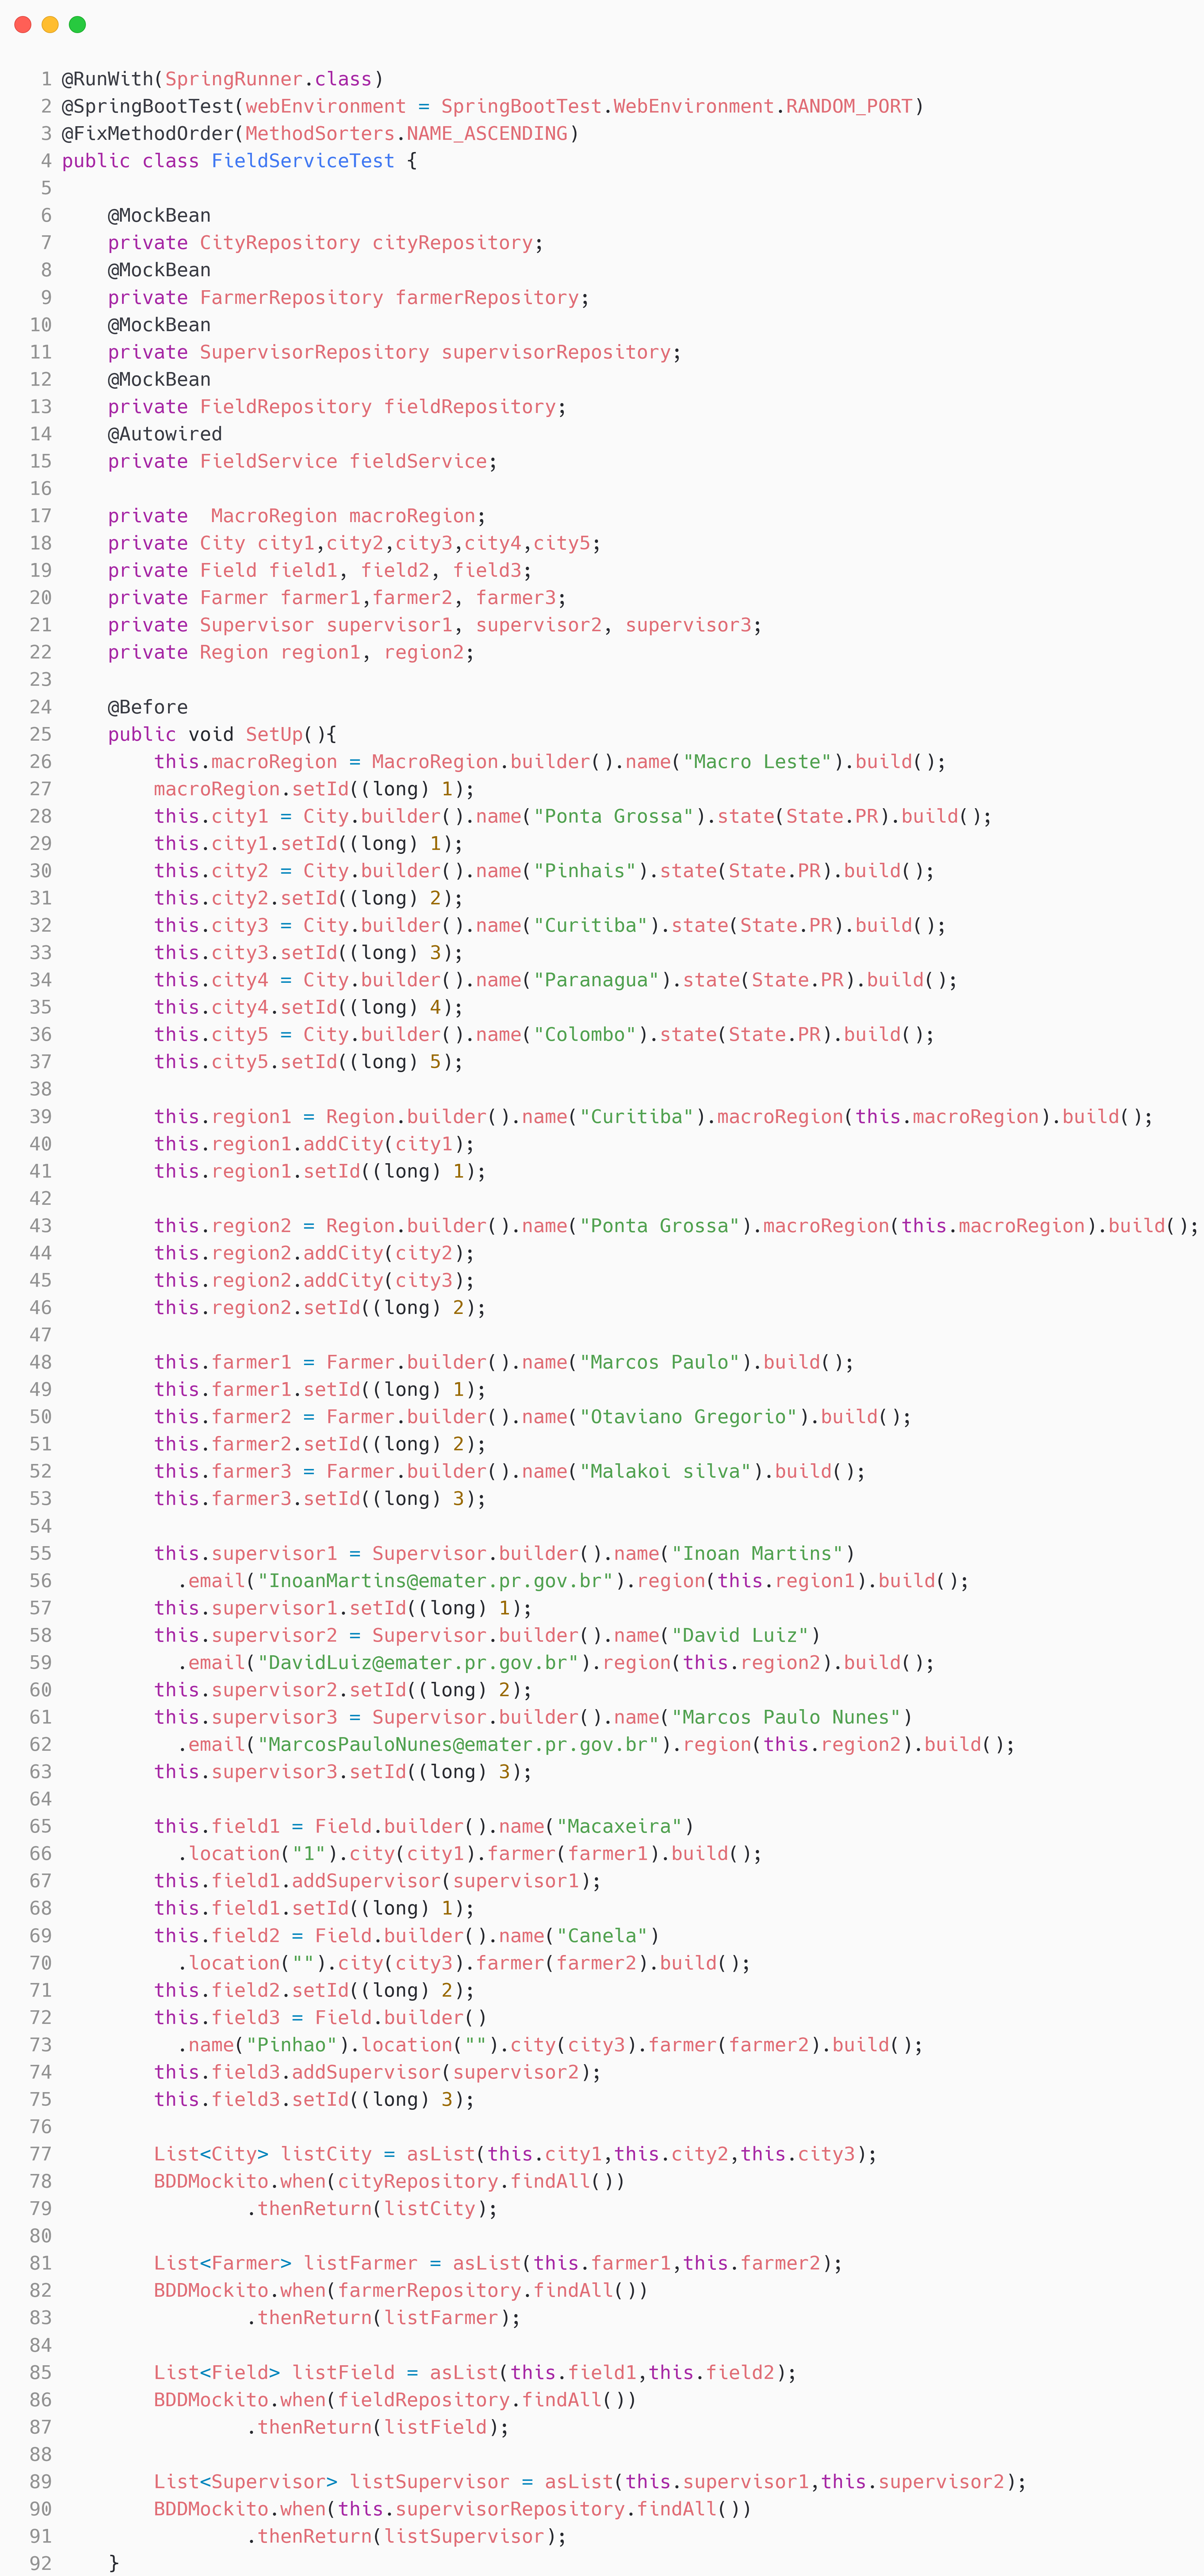
\includegraphics[scale=0.13]{dados/figuras/carbonFieldServicebuild.png}
\end{figure}

\begin{figure}[H]
	\centering
	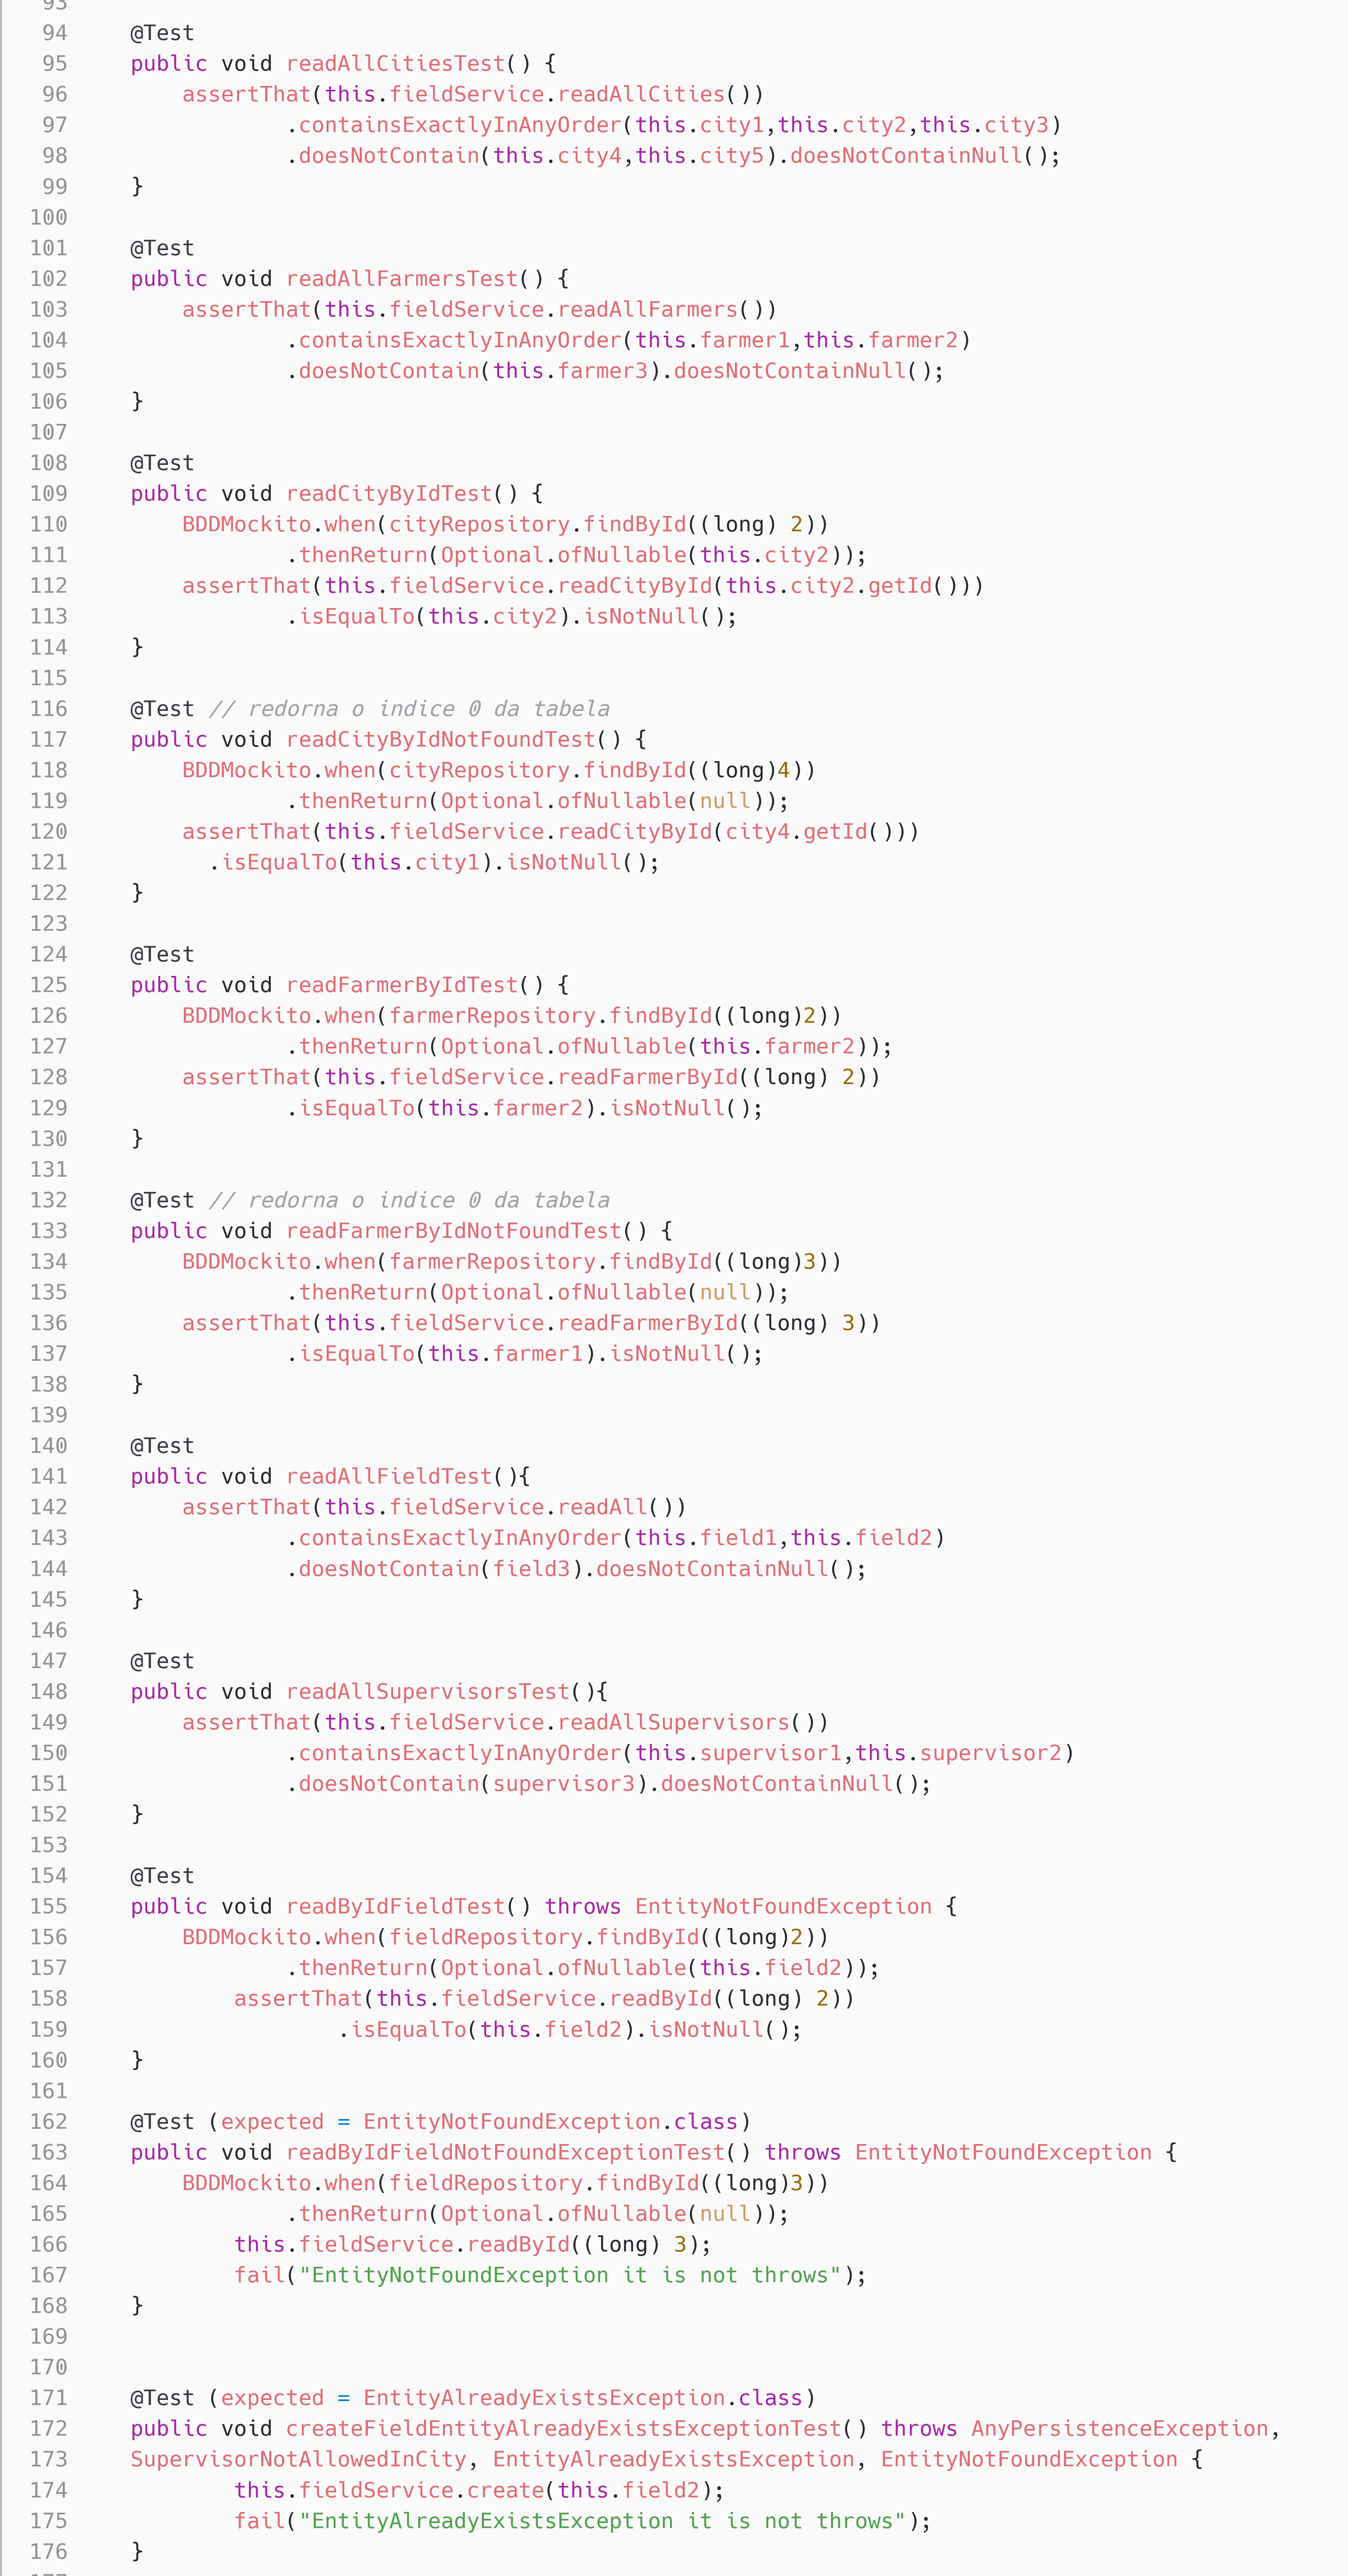
\includegraphics[scale=0.14]{dados/figuras/carbonFieldService1.png}
\end{figure}

\begin{figure}[H]
	\centering
	\includegraphics[scale=0.13]{dados/figuras/carbonFieldService2.png}
\end{figure}

\begin{figure}[H]
	\centering
	\includegraphics[scale=0.13]{dados/figuras/carbonFieldService3.png}
	\caption{Classe de Teste  FieldService.java.}
	\label{testeFieldService}
\end{figure}

 \item O método \textit{“setUp”} que tem sua declaração na linha 25 e vai até a linha 92 é responsável por realizar a construção dos objetos declarados nas linhas 17 a 21.

\item O método  \textit{“setUp”} também é responsável por construir algumas funcionalidades para os objetos do tipo Mock:

\begin{itemize}

 \item Linha  78 é definido que toda vez que o comando \textit{“cityRepository.findAll()”} for chamado o retorno será uma lista do tipo “\textit{City}” definida na linha 77;
\item Linha  82 é definido que toda vez que o comando \textit{“farmerRepository.findAll()”} for chamado o retorno será uma lista do tipo “\textit{Farmer}” definida na linha 81;
\item Linha  86 é definido que toda vez que o comando \textit{“fieldRepository.findAll()”} for chamado o retorno será uma lista do tipo \textit{Field} definida na linha 85;
\item Linha  90 é definido que toda vez que o comando\textit{ “supervisorRepository.findAll()”} for chamado o retorno será uma lista do tipo “\textit{City}” definida na linha 89;
\end{itemize}{}
\end{itemize}{}


A FIGURA \ref{testeFieldService} tambem apresenta os casos de testes criados para a classe \textit{FieldTest}. 


A ideia geral na elaboração dos testes é a de cobrir cada atribuição de dados, as entrada e saída de dados da classe \textit{FieldService}, buscando a cobertura de 100\% das linhas métodos e atributo da classe. Os resultados obtidos da execução dos testes foram listados a seguir:


Método de teste \textit{readAllCitiesTest ()} linhas 94 a 99 figura \ref{testeFieldService}: Este teste lista todas as cidades do banco de dados. Não há entrada de dados. A Saída é uma lista do tipo \textit{“City”} contendo as cidades salvas na base de dados. Nesta assertiva o método testado deve retornar a lista criada na linha 77, que contem 3 objetos do tipo cidade correspondentes a comparação.

Método de teste \textit{ readAllFarmersTest ()} linhas 101 a 106 figura \ref{testeFieldService}: Este teste lista todos os agricultores do banco de dados. Não há entrada de dados. A Saída é uma lista do tipo \textit{“Farmer”} contendo agricultores salvos na base de dados. Nesta assertiva o método testado deve retornar a lista criada na linha 81, que contem 2 objetos do tipo agricultor correspondentes a comparação.

Método de teste \textit{ readCityByIdTest ()} linhas 108 a 114 figura \ref{testeFieldService}: Este teste busca uma cidade na base de dados pelo seu identificador único. A entrada consiste em um numeral do tipo \textit{“Long”}. A saída é um objeto do tipo \textit{“City”}. Nesta assertiva o método testado deve retornar o registro \textit{mocado} nas linhas 110 e 111, o qual corresponde ao objeto comparado. 

Método de teste \textit{ readCityByIdNotFoundTest ()} linhas 116 a 122 figura \ref{testeFieldService}: Este teste busca uma cidade na base de dados pelo seu identificador único. A entrada consiste em um numeral do tipo \textit{“Long”}. A saída é um objeto do tipo \textit{“City”}. Nesta assertiva o método testado deve retornar o índice zero da lista criada na linha 77, o qual corresponde ao objeto comparado.

Método de teste \textit{ readFarmerByIdTest ()} linhas 124 a 130 figura \ref{testeFieldService}: Este teste busca um agricultor na base de dados pelo seu identificador único. A entrada consiste em um numeral do tipo \textit{“Long”}. A saída é um objeto do tipo \textit{“Farmer”}. Nesta assertiva o método testado deve retornar o registro \textit{mocado} nas linhas 126 e 127, o qual corresponde ao objeto comparado.

Método de teste \textit{ readFarmerByIdNotFoundTest ()} linhas 132 a 138 figura \ref{testeFieldService}: Este teste busca um agricultor na base de dados pelo seu identificador único. A entrada consiste em um numeral do tipo \textit{“Long”}. A saída é um objeto do tipo \textit{“Farmer”}. Nesta assertiva o método testado deve retornar o índice zero da lista criada na linha 81, o qual corresponde ao objeto comparado.


Método de teste \textit{ readAllFieldTest ()} linhas 140 a 145 figura \ref{testeFieldService}: Este teste busca os registros do tipo \textit{Field} na base de dados. Não há entrada de dados.  A saída é uma lista do tipo \textit{Field}. Nesta assertiva o método testado deve retornar a lista criada na linha 85, que contem dois registros correspondentes a comparação.

Método de teste \textit{readAllSupervisorsTest ()} linhas 147 a 152 figura \ref{testeFieldService}: Este teste busca os registros do tipo \textit{“Supervisor”} na base de dados. Não há entrada de dados.  A saída é uma lista do tipo \textit{“Supervisor”}. Nesta assertiva o método testado deve retornar a lista criada na linha 89, que contém dois registros correspondentes a comparação.

Método de teste \textit{ readByIdFieldTest ()} linhas 154 a 160 figura \ref{testeFieldService}: Este teste busca um registro do tipo \textit{Field} na base de dados pelo seu identificador único. A entrada consiste em um numeral do tipo \textit{“Long”}. A saída é um objeto do tipo \textit{Field}. Nesta assertiva o método testado deve retornar o objeto \textit{mocado} nas linhas 156 e 157, o qual corresponde ao objeto comparado.

Método de teste \textit{ readByIdFieldNotFoundExceptionTest ()} linhas 162 a 168 figura \ref{testeFieldService}: Este teste busca um registro do tipo \textit{Field} na base de dados pelo seu identificador único, quando não encontrado é gerada uma exceção. A entrada consiste em um numeral do tipo \textit{“Long”}. A saída é uma exceção do tipo \textit{“EntityNotFoundException”}. Nesta assertiva o método testado deve retornar uma exceção, ao buscar um objeto pelo índice passado como parâmetro, ao realizar a consulta no banco um registro vazio é retornado, o que é simulado nas linhas 164 e 165, o que garante o lançamento da exceção \textit{“EntityNotFoundException”}.


Método de teste \textit{ createFieldEntityAlreadyExistsExceptionTest ()} linhas 171 a 176 figura \ref{testeFieldService}:  Este teste consiste em tentar criar um novo registro do tipo \textit{Field}, mas o item a ser criado é identificado como já existente na base de dados. A Entrada consiste em um objeto do tipo \textit{Field}. A Saída é o lançamento da exceção \textit{“EntityAlreadyExistsException”}. A assertiva tenta inserir um registro que já se encontra na base de dados simulada pela linha 85, o que proporciona o lançamento da exceção.  

Método de teste \textit{ deleteFieldTest ()} linhas 178 a 187 figura \ref{testeFieldService}: Este teste consiste em deletar um registro do tipo \textit{Field}. A Entrada consiste em um objeto do tipo \textit{Field}. Não há saída de dados.  A assertiva deleta um registro do banco linha 183, a validação é feita ao tentar consultar por este registro no banco simulado, o retorno é o índice zero do banco e não o procurado.  

Método de teste \textit{ deleteFieldNotFoundExceptionTest ()} linhas 189 a 197 figura \ref{testeFieldService}: Este teste consiste em deletar um registro do tipo \textit{Field}, mas o item a ser deletado não existe na base de dados. A Entrada consiste em um objeto do tipo \textit{Field}. A Saída é o lançamento da exceção \textit{“EntityNotFoundException”}. A assertiva tenta deletar um registro, mas ao consultar o registro na base de dados simulada pela linha 192 o retorno é um nulo pois ele não existe na base, há o lançamento da exceção.  

Método de teste \textit{ deleteFieldUseEntityInUseExceptionTest ()} linhas 199 a 206 figura \ref{testeFieldService}: Este teste consiste em deletar um registro do tipo \textit{Field}, mas o item a ser deletado está sendo utilizado na base de dados. A Entrada consiste em um objeto do tipo \textit{Field}. A Saída é o lançamento da exceção \textit{“UseEntityInUseException”}. A assertiva tenta deletar um registro, mas este está sendo utilizado na base de dados simulada pela linha 203, há o lançamento da exceção.  

Método de teste \textit{ updateFieldNotFoundExceptionTest ()} linhas 208 a 214 figura \ref{testeFieldService}: Este teste consiste em atualizar um registro do tipo \textit{Field}, mas o item a ser atualizado não existe na base de dados. A Entrada consiste em um objeto do tipo \textit{Field}. A Saída é o lançamento da exceção \textit{“EntityNotFoundException”}. A assertiva tenta atualizar um registro, mas ao consultar o registro na base de dados simulada pela linha 211 o retorno é um nulo pois ele não existe na base, há o lançamento da exceção.  

Método de teste \textit{ updateFieldSupervisorNotAllowedInCityTest ()} linhas 216 a 223 figura \ref{testeFieldService}: Este teste consiste em tentar atualizar um registro do tipo \textit{Field}, mas é identificado que os supervisores presentes no registro não pertencem a cidade que compõe o registro. A Entrada consiste em um objeto do tipo \textit{Field}. A Saída é o lançamento da exceção \textit{“SupervisorNotAllowedInCity”}. A assertiva tenta atualizar um registro que possui supervisores que não se localizam na cidade do registro linha 219, o que proporciona o lançamento da exceção.  


Método de teste \textit{ deleteFieldAnyPersistenceExceptionTest ()} linhas 225 a 232 figura \ref{testeFieldService}: Este teste consiste em deletar um registro do tipo \textit{Field}, mas o item a ser deletado gera um erro na base de dados. A Entrada consiste em um objeto do tipo \textit{Field}. A Saída é o lançamento da exceção \textit{“AnyPersistenceException”}. A assertiva tenta deletar um registro, mas um erro é gerado, há o lançamento da exceção.  

Método de teste \textit{ updateFieldTest ()} linhas 234 a 272 figura \ref{testeFieldService}: Este teste consiste em atualizar um registro do tipo \textit{Field}. A Entrada consiste em um objeto do tipo \textit{Field}. Não há saída de dados. As assertivas consistem em recuperar um objeto da base de dados simulada linha 237, atualizar os campos deste objeto linhas 254 a 259, e em seguida atualizar esse registro na base linha 240. Caso não haja o lançamento de uma exceção o objeto atualizado é recuperado da base simulada, linha 264, e em seguida é feita as assertivas dos dados atualizados.

Método de teste \textit{ updateFieldAnyPersistenceExceptionTest ()} linhas 274 a 290 figura \ref{testeFieldService}: Este teste consiste em atualizar um registro do tipo \textit{Field}, mas o item a ser atualizado possui um agricultor nulo. A Entrada consiste em um objeto do tipo \textit{Field}. A Saída é o lançamento da exceção \textit{“AnyPersistenceException”}. A assertiva tenta atualizar um registro, mas ao consultar o agricultor na base de dados simulada pela linha 283 o retorno é um nulo, há o lançamento da exceção.  

Método de teste \textit{ createFieldSupervisorNotAllowedInCityTest ()} linhas 293 a 305 figura \ref{testeFieldService}: Este teste consiste em tentar criar um novo registro do tipo \textit{Field}, mas é identificado que os supervisores presentes no registro não pertencem a cidade que compõe o registro. A Entrada consiste em um objeto do tipo \textit{Field}. A Saída é o lançamento da exceção \textit{“SupervisorNotAllowedInCity”}. A assertiva tenta inserir um registro que possui supervisores que não se localizam na cidade do registro linha 296, o que proporciona o lançamento da exceção.  

Método de teste \textit{ createFieldTest ()} linhas 307 a 329 figura \ref{testeFieldService}: Este teste consiste em criar um novo registro do tipo \textit{Field} na base de dados. A Entrada consiste em um objeto do tipo \textit{Field}. O método não gera uma saída. A validação é feita através de um \textit{try cath}, que captura qualquer exceção que ocorra ao salvar o objeto. Como o método não lança uma exceção ele é aceito. A assertiva, no entanto, é feita através do repositório \textit{mocado} linhas 321 e 322, depois de inserido é simulada uma consulta pelo identificador único do objeto inserido anteriormente o qual deve retornar o objeto que acaba de ser inserido. 

Método de teste \textit{ createFieldAnyPersistenceExceptionTest ()} linhas 331 a 345 figura \ref{testeFieldService}: Este teste consiste em tentar criar um novo registro do tipo \textit{Field}, mas o item a ser criado gera algum erro na base de dados. A Entrada consiste em um objeto do tipo \textit{Field}. A Saída é o lançamento da exceção \textit{“AnyPersistenceException”}. A assertiva tenta inserir um registro na base de dados simulada pela linha 338, o que proporciona o lançamento da exceção.  

Método de teste \textit{ updateFieldEntityAlreadyExistsExceptionTest ()} linhas 347 a 360 figura \ref{testeFieldService}: Este teste consiste em tentar atualizar um registro do tipo \textit{Field}, mas o item a ser atualizado é identificado como já existente na base de dados. A Entrada consiste em um objeto do tipo \textit{Field}. A Saída é o lançamento da exceção \textit{“EntityAlreadyExistsException”}. A assertiva tenta inserir um registro que já se encontra na base de dados simulada pela linha 351, neste caso foi necessário duplicar o registro a ser atualizado para que o lançamento da exceção fosse forçado.  

Após a execução dos testes a cobertura das entradas e saídas de dados da classe FieldService.java é de 100\%.


 \subsection{RESULTADO DOS TESTES CLASSE SURVEYSERVICE.JAVA}

A classe \textit{SurveyService} é responsável por realizar a comunicação com a classe \textit{Survey}, e com as demais classes que a compõem. A FIGURA \ref{packFieldService} apresenta o diagrama de classes da classe \textit{SurveyService} e as demais classes que a compõem assim como a classe responsável por realizar os testes de seus métodos e variáveis. Também é possível analisar no diagrama os atributos e métodos que pertence à classe \textit{SurveyService}, assim como os métodos e atributos da classe de \textit{SurveyServiceTest}.  


A classe de teste apresentada na FIGURA \ref{packFieldService} possui vinte e quatro métodos de teste é um método de apoio aos testes denominado \textit{“setUp”}, o objetivo dos testes é exercitar a classe \textit{SurveyService} até que todos as variáveis, entradas e saídas de dados sejam executados pelo menos uma vez. Como a classe \textit{SurveyService} trabalha com outras classes além da \textit{Survey} se faz necessário a instanciação destas como: \textit{Supervisor}, \textit{Farmer}, \textit{City} e outras para a execução completa dos testes. Como a classe trabalha com entidades que serão persistidas em um banco de dados, foi preciso criar uma referência para a interface \textit{SurveyRepository} e outros repositórios que são chamados durante a execução dos testes. Como o objetivo deste trabalho é cobrir o sistema com testes unitários e testes que integram classes entidades com o banco de dados ou comunicação com APIs são testes de integração foi utilizado “\textit{MOCKs}” para simular o comportamento dos repositórios.

 \begin{figure}[H]
	\centering
	\includegraphics[scale=0.4]{dados/figuras/PackagesurveyService.png}
	\caption{Diagrama de classes SurveyServiceTest.java.}
	\label{packFieldService}
\end{figure}


A FIGURA \ref{testeSurveyService} apresenta a declaração da classe de teste, os atributos utilizados para desenvolver os testes e o método\textit{ “setUp”} utilizado para preparar o ambiente para os testes.

O trecho de código da FIGURA \ref{testeSurveyService} apresenta as seguintes funcionalidades:


\begin{itemize}

\item Linha 1 A anotação \textit{@RunWith} permite a execução dos testes dentro de um contexto do \textit{Spring}. O comando \textit{SpringRunner}.class fornece suporte para carregar um \textit{Spring}\textit{ApplicationContext} e ter \textit{beans }\textit{@Autowired} na instância de teste.

\item Na linha 2 é utilizada a anotação \textit{@SpringBootTest} que prepara um contexto \textit{Spring} e inclui a possibilidade de iniciar um container em um porta default ou configurada pelo usuário. Neste caso a porta foi definida de forma randômica através do comando \textit{“SpringBootTest.WebEnvironment.RANDOM\_PORT”}; 

 \item Na linha 3 é utilizada a anotação \textit{@FixMethodOrder} que permite definir uma ordem de execução dos testes, neste casso foi definida a ordem \textit{“NAME\_ASCENDING"} que faz a execução dos testes de acordo com o nome de maneira ascendente;

 \item Linha 4 a classe \textit{SurveyServiceTest} é aberta;

 \item Da linha 6 a 11 há a declaração dos objetos \textit{MOCKs} que serão utilizadas para a comunicação com o banco de dados. A anotação \textit{@MockBean} foi utilizada na declaração destas variáveis, ela permite que caso exista um \textit{bean }compatível com a classe declarada no contexto da aplicação \textit{Spring} este \textit{bean }será substituído por um \textit{Mock};

\item Linhas 13 e 14 uma instancia da classe SurveyService é declarada, a anotação \textit{@Autowired} é utilizada para a injeção automática de um \textit{bean }correspondente ao declarado na variável. 
 
\item Da linha 16 a 21 há a declaração dos objetos que serão utilizados nos testes;

 \item Na linha 23 é utilizado a anotação \textit{@Before}, esta anotação determina que sempre antes da execução de um teste o método \textit{“setUp”} deve ser executado primeiro.

 \item O método \textit{“setUp”} que tem sua declaração na linha 24 e vai até a linha 108 é responsável por realizar a construção dos objetos declarados nas linhas 16 a 21.

\item O método  \textit{“setUp”} também é responsável por construir algumas funcionalidades para os objetos do tipo \textit{Mock}:

\begin{itemize}

 \item Linha  107 é definido que toda vez que o comando \textit{“surveyRepository.findAll()”} for chamado o retorno será uma lista do tipo “\textit{Survey}” definida na linha 106;
\end{itemize}{}
\end{itemize}{}


A FIGURA \ref{testeSurveyService} também apresenta os casos de testes criados para a classe \textit{SurveyService}. 


A ideia geral na elaboração dos testes é a de cobrir cada atribuição de dados, as entradas e saída de dados da classe \textit{ SurveyService}, buscando a cobertura de 100\% das linhas métodos e atributo da classe. Os resultados obtidos da execução dos testes foram listados a seguir:


Método de teste \textit{ readAllSurveyTest()} linhas 110 a 115 figura \ref{testeSurveyService}: Este teste lista todas as pesquisas do banco de dados. Não há entrada de dados. A Saída é uma lista do tipo \textit{“Survey”} contendo as pesquisas salvas na base de dados. Nesta assertiva o método testado deve retornar a lista criada na linha 106, que contem 2 objetos do tipo survey correspondentes a comparação.


\begin{figure}[H]
	\centering
	\includegraphics[scale=0.13]{dados/figuras/carbonFieldServicebuild.png}
\end{figure}

\begin{figure}[H]
	\centering
	\includegraphics[scale=0.25]{dados/figuras/carbonSurveyService1.png}
\end{figure}

\begin{figure}[H]
	\centering
	\includegraphics[scale=0.26]{dados/figuras/carbonSurveyService2.png}
\end{figure}

\begin{figure}[H]
	\centering
	\includegraphics[scale=0.27]{dados/figuras/carbonSurveyService3.png}
	\caption{Classe de Teste  SurveyServiceTest.java.}
	\label{testeSurveyService}
\end{figure}

Método de teste \textit{ readByIdSurveyTest ()} linhas 117 a 123 figura \ref{testeSurveyService}: Este teste busca uma pesquisa na base de dados pelo seu identificador único. A entrada consiste em um numeral do tipo \textit{“Long”}. A saída é um objeto do tipo \textit{“Survey”}. Nesta assertiva o método testado deve retornar o registro \textit{mocado} nas linhas 119 e 120, o qual corresponde ao objeto comparado.

Método de teste \textit{ readByIdSurveyEntityNotFoundExceptionTest ()} linhas 125 a 131 figura \ref{testeSurveyService}: Este teste busca um registro do tipo \textit{“Survey”} na base de dados pelo seu identificador único, quando não encontrado é gerada uma exceção. A entrada consiste em um numeral do tipo \textit{“Long”}. A saída é uma exceção do tipo \textit{“EntityNotFoundException”}. Nesta assertiva o método testado deve retornar uma exceção, ao buscar um objeto pelo índice passado como parâmetro, ao realizar a consulta no banco um registro vazio é retornado, o que é simulado nas linhas 127 e 128, o que garante o lançamento da exceção \textit{“EntityNotFoundException”}.

Método de teste \textit{ readFieldbyIdTest ()} linhas 133 a 139 figura \ref{testeSurveyService}: Este teste busca um registro do tipo \textit{Field} na base de dados pelo seu identificador único. A entrada consiste em um numeral do tipo \textit{“Long”}. A saída é um objeto do tipo \textit{Field}. Nesta assertiva o método testado deve retornar o objeto \textit{mocado} nas linhas 135 e 136, o qual corresponde ao objeto comparado.

Método de teste \textit{ readFieldbyIdEntityNotFoundExceptionTest ()} linhas 141 a 147 figura \ref{testeSurveyService}: Este teste busca um registro do tipo \textit{Field} na base de dados pelo seu identificador único, quando não encontrado é gerada uma exceção. A entrada consiste em um numeral do tipo \textit{“Long”}. A saída é uma exceção do tipo \textit{“EntityNotFoundException”}. Nesta assertiva o método testado deve retornar uma exceção, ao buscar um objeto pelo índice passado como parâmetro, ao realizar a consulta no banco um registro vazio é retornado, o que é simulado nas linhas 143 e 144, o que garante o lançamento da exceção \textit{“EntityNotFoundException”}.

Método de teste \textit{ readHarvestByIdTest ()} linhas 150 a 157 figura \ref{testeSurveyService}: Este teste busca um registro do tipo \textit{“Harvest”} na base de dados pelo seu identificador único. A entrada consiste em um numeral do tipo \textit{“Long”}. A saída é um objeto do tipo \textit{“Harvest”}. Nesta assertiva o método testado deve retornar o objeto \textit{mocado} nas linhas 152 e 153, o qual corresponde ao objeto comparado.

Método de teste \textit{ readHarvestByIdEntityNotFoundExceptionTest ()} linhas 159 a 165 figura \ref{testeSurveyService}: Este teste busca um registro do tipo \textit{“Harvest”} na base de dados pelo seu identificador único, quando não encontrado é gerada uma exceção. A entrada consiste em um numeral do tipo \textit{“Long”}. A saída é uma exceção do tipo \textit{“EntityNotFoundException”}. Nesta assertiva o método testado deve retornar uma exceção, ao buscar um objeto pelo índice passado como parâmetro, ao realizar a consulta no banco um registro vazio é retornado, o que é simulado nas linhas 161 e 161, o que garante o lançamento da exceção \textit{“EntityNotFoundException”}.

Método de teste \textit{ readAllFieldsTest ()} linhas 167 a 175 figura \ref{testeSurveyService}: Este teste busca os registros do tipo \textit{Field} na base de dados. Não há entrada de dados.  A saída é uma lista do tipo \textit{Field}. Nesta assertiva o método testado deve retornar a lista criada na linha 169, que contém dois registros correspondentes a comparação.

Método de teste \textit{ readAllHarvestsTest ()} linhas 177 a 185 figura \ref{testeSurveyService}:  Este teste busca os registros do tipo \textit{“Harvest”} na base de dados. Não há entrada de dados.  A saída é uma lista do tipo \textit{“Harvest”}. Nesta assertiva o método testado deve retornar a lista criada na linha 179, que contém dois registros correspondentes a comparação.

Método de teste \textit{ readAllFieldsOutOfCurrentHarvestTest ()} linhas 187 a 195 figura \ref{testeSurveyService}: Este teste busca os registros do tipo \textit{Field} na base de dados que pertencem a colheita. A entrada é um numeral do tipo \textit{“Long”} identificador único de uma colheita.  A saída é uma lista do tipo \textit{Field} contendo os registros que pertencem a colheita. Nesta assertiva o método testado deve retornar a lista criada na linha 189, que contém um registro correspondente a comparação.

Método de teste \textit{ readByHarvestIdTest ()} linhas 197 a 201 figura \ref{testeSurveyService}: Este teste lista todas as pesquisas do banco de dados que contém uma determinada colheita. A entrada é um numeral do tipo \textit{“Long”} identificador único de uma colheita. A Saída é uma lista do tipo \textit{“Survey”} contendo as pesquisas salvas na base de dados que contem a colheita. Nesta assertiva o método testado deve retornar a lista criada na linha 106, que contem 2 objetos do tipo \textit{survey} correspondentes a comparação.

Método de teste \textit{ readByHarvestIdEntityNotFoundExceptionTest ()} linhas 205 a 209 figura \ref{testeSurveyService}: Este teste lança uma exceção do tipo \textit{“EntityNotFoundException”} quando não encontra uma pesquisa que contenha a colheita. A entrada é um numeral do tipo \textit{“Long”} identificador único de uma colheita. A Saída é uma exceção do tipo \textit{“EntityNotFoundException”}. Nesta assertiva o método testado deve lançar uma exceção do tipo \textit{“EntityNotFoundException”}.

Método de teste \textit{ deleteSurveyEntityNotFoundExceptionTest ()} linhas 211 a 218 figura \ref{testeSurveyService}: Este teste consiste em deletar um registro do tipo \textit{“Survey”}, mas o item a ser deletado não existe na base de dados. A Entrada consiste em um objeto do tipo \textit{“Survey”}. A Saída é o lançamento da exceção \textit{“EntityNotFoundException”}. A assertiva tenta deletar um registro, mas ao consultar o registro na base de dados simulada pelas linhas 214 e 215 o retorno é um nulo pois ele não existe na base, há o lançamento da exceção.  

Método de teste \textit{ deleteSurveyEntityInUseExceptionTest ()} linhas 220 a 228 figura \ref{testeSurveyService}: Este teste consiste em deletar um registro do tipo \textit{“Survey”}, mas o item a ser deletado está sendo utilizado na base de dados. A Entrada consiste em um objeto do tipo \textit{“Survey”}. A Saída é o lançamento da exceção \textit{“UseEntityInUseException”}. A assertiva tenta deletar um registro, mas este está sendo utilizado na base de dados simulada pela linha 225, há o lançamento da exceção.  

Método de teste \textit{ deleteSurveyAnyPersistenceExceptionTest ()} linhas 230 a 238 figura \ref{testeSurveyService}: Este teste consiste em deletar um registro do tipo \textit{“Survey”}, mas o item a ser deletado gera um erro na base de dados. A Entrada consiste em um objeto do tipo \textit{“Survey”}. A Saída é o lançamento da exceção \textit{“AnyPersistenceException”}. A assertiva tenta deletar um registro, mas um erro é gerado, há o lançamento da exceção.

Método de teste \textit{ deleteSurveyTest ()} linhas 240 a 255 figura \ref{testeSurveyService}: Este teste consiste em deletar um registro do tipo \textit{“Survey”}. A Entrada consiste em um objeto do tipo \textit{“Survey”}. Não há saída de dados.  A assertiva deleta um registro do banco linha 245, a validação é feita ao tentar consultar este registro no banco simulado e o retorno é uma exceção do tipo \textit{“EntityNotFoundException”}.  

Método de teste \textit{ createSurveyEntityNotFoundExceptionFieldTest ()} linhas 257 a 265 figura \ref{testeSurveyService}: Este teste consiste em criar um registro do tipo \textit{“Survey”}, mas o item a ser atualizado não possui um \textit{Field}. A Entrada consiste em um objeto do tipo \textit{“Survey”}. A Saída é o lançamento da exceção \textit{“EntityNotFoundException”}. A assertiva tenta criar um registro, mas ao buscar um registro do tipo \textit{Field} na base de dados simulada pela linha 261 o retorno é um nulo pois ele não existe na base, há o lançamento da exceção.  

Método de teste \textit{ createSurveyEntityAlreadyExistsExceptionTest ()} linhas 267 a 272 figura \ref{testeSurveyService}: Este teste consiste em tentar criar um novo registro do tipo \textit{“Survey”}, mas o item a ser criado é identificado como já existente na base de dados. A Entrada consiste em um objeto do tipo \textit{“Survey”}. A Saída é o lançamento da exceção \textit{“EntityAlreadyExistsException”}. A assertiva tenta inserir um registro que já se encontra na base de dados simulada pela linha 106, o que proporciona o lançamento da exceção.  

Método de teste \textit{ createSurveyEntityNotFoundExceptionHarversTest ()} linhas 274 a 284 figura \ref{testeSurveyService}: Este teste consiste em criar um registro do tipo \textit{“Survey”}, mas o item a ser atualizado não possui uma colheita. A Entrada consiste em um objeto do tipo \textit{“Survey”}. A Saída é o lançamento da exceção \textit{“EntityNotFoundException”}. A assertiva tenta atualizar um registro, mas ao buscar um registro do tipo \textit{“Harvest”} na base de dados simulada pela linha 280 o retorno é um nulo pois ele não existe na base, há o lançamento da exceção.  

Método de teste \textit{ createSurveyTest ()} linhas 286 a 302 figura \ref{testeSurveyService}: Este teste consiste em criar um novo registro do tipo \textit{“Survey”} na base de dados. A Entrada consiste em um objeto do tipo \textit{“Survey”}. O método não gera uma saída. A validação é feita através de um \textit{try cath}, que captura qualquer exceção que ocorra ao salvar o objeto. Como o método não lança uma exceção ele é aceito. A assertiva, no entanto, é feita através do repositório \textit{mocado} linhas 295 e 296, depois de inserido é simulada uma consulta pelo identificador único do objeto inserido o qual deve retornar o objeto que acaba de ser inserido.

Método de teste \textit{ createSurveyAnyPersistenceExceptionTest ()} linhas 304 a 315 figura \ref{testeSurveyService}: Este teste consiste em tentar criar um novo registro do tipo \textit{“Survey”}, mas o item a ser criado gera algum erro na base de dados. A Entrada consiste em um objeto do tipo \textit{“Survey”}. A Saída é o lançamento da exceção \textit{“AnyPersistenceException”}. A assertiva tenta inserir um registro na base de dados simulada pela linha 312, o que proporciona o lançamento da exceção.

Método de teste \textit{ updateSurveyEntityNotFoundExceptionTest ()} linhas 317 a 325 figura \ref{testeSurveyService}: Este teste consiste em atualizar um registro do tipo \textit{“Survey”}, mas o item a ser atualizado não existe na base de dados. A Entrada consiste em um objeto do tipo \textit{“Survey”}. A Saída é o lançamento da exceção \textit{“EntityNotFoundException”}. A assertiva tenta atualizar um registro, mas ao consultar o registro na base de dados simulada pela linha 321 o retorno é um nulo pois ele não existe na base, há o lançamento da exceção.  

Método de teste \textit{ updateSurveyAnyPersistenceExceptionTest ()} linhas 327 a 337 figura \ref{testeSurveyService}: Este teste consiste em atualizar um registro do tipo \textit{“Survey”}, mas o item a ser alterado gera um erro na base de dados. A Entrada consiste em um objeto do tipo \textit{“Survey”}. A Saída é o lançamento da exceção \textit{“AnyPersistenceException”}. A assertiva tenta atualizar um registro, mas ao alterar a base de dados simulada pela linha 332 o retorno é um exceção, há o lançamento da exceção.

Método de teste \textit{ updateSurveyTest ()} linhas 339 a 375 figura \ref{testeSurveyService}: Este teste consiste em atualizar um registro do tipo \textit{“Survey”}. A Entrada consiste em um objeto do tipo \textit{“Survey”}. Não há saída de dados. As assertivas consistem em recuperar um objeto da base de dados simulada linha 342, atualizar os campos deste objeto linhas 358 e 359, e em seguida atualizar esse registro na base linha 344. Caso não haja o lançamento de uma exceção o objeto atualizado é recuperado da base simulada, linha 361, e em seguida é feita as assertivas dos dados atualizados.

Após a execução dos testes a cobertura das entradas e saídas de dados da classe \textit{SurveyService}.java é de 100\%.



\subsection{RESULTADO GERAL DOS TESTES PACOTE SERVICE}

Para alcançar a cobertura de 100\% de todos os métodos linhas e classes do pacote Service foram criados no total 294 testes de unidade, onde 283 foram aprovados, 5 ignorados e 6 rejeitado. Cada classe possui o seguinte número de casos de teste: 

\begin{itemize}
        \item Pacote Base:
\begin{itemize}
    \item Classe \textit{FieldServiceTest}: 23 casos de teste aprovados;
    \item Classe \textit{RegionServiceTest}: 18 casos de teste aprovados, 1 reprovado;
    \item Classe \textit{FarmerServiceTest}: 12 casos de teste aprovados, 2 reprovados;
    \item Classe \textit{LocalDateTimeConverterTest}: 2 casos de teste aprovados;
    \item Classe \textit{MacroRegionServiceTest}: 12 casos de teste aprovados, 2 reprovados;
    \item Classe \textit{CityServiceTest}: 3 casos de teste aprovados;
    \item Classe \textit{SupervisorServiceTest}: 16 casos de teste aprovados, 1 reprovado;
\end{itemize}
  \item Pacote MIP:
  \begin{itemize} 
    \item Classe \textit{PestDiseaseServiceTest}: 14 casos de teste aprovados;
    \item Classe \textit{PestNaturalPredatorServiceTest}: 14 casos de teste aprovados; 
    \item Classe \textit{PestServiceTest}: 14 casos de teste aprovados;
    \item Classe \textit{MIPSampleServiceTest}: 18 casos de teste aprovados, 1 ignorado;
\end{itemize}
  \item Pacote \textit{Survey}:
  \begin{itemize}   
    \item Classe \textit{SurveyServiceTest}: 23 casos de teste aprovados, 1 ignorado;
    \item Classe \textit{HarvestServiceTest}: 14 casos de teste aprovados;
\end{itemize}
  \item Pacote MID:
  \begin{itemize}
    \item Classe \textit{BladeReadingResponsibleEntityServiceTest}: 18 casos de teste aprovados;
    \item Classe \textit{MIDRustSampleServiceTest}: 13 casos de teste aprovados;
    \item Classe \textit{BladeReadingResponsiblePersonServiceTest}: 18 casos de teste aprovados;
    \end{itemize}
    \item Pacote \textit{Pulverisation}:
  \begin{itemize}
    \item Classe \textit{ProductServiceTest}: 17 casos de teste aprovados, 1 ignorado;
    \item Classe \textit{PulverisationOperationServiceTest}: 20 casos de teste aprovados, 1 ignorado;
    \item Classe \textit{TargetServiceTest}: 14 casos de teste aprovados, 1 ignorado;
    \end{itemize}
    \end{itemize}



Como já dito anterior mente os testes podem garantir que o software é livre de defeitos mais, mas seu objetivo principal é revelar a presença de defeitos. Após a execução dos testes a taxa de cobertura foi de: 100\% das classes, 100\% dos métodos e 98\% das linhas. Como alguns casos de testes falharam não foi possível a cobertura de 100\% das linhas.


\section{TESTE IGNORADOS E REPROVADOS}

Em resumo, foram produzidos 652 testes de unidade, buscando a cobertura de 100\% das linhas, variáveis e métodos dos pacotes\textit{Entity}e Service do aplicativo MIP. Dentre eles 640 foram aprovados o equivalente a 98,16\% dos testes, 5 testes equivalente a 0,77\% foram ignorados e 7 falharam o que corresponde a 1,07\%.

\subsection{REPROVADOS}

Dos testes 7 casos falharam, os casos falhos e os motivos pelo qual falharam são listados a seguir:

  \begin{itemize}
    \item Pacote\textit{Entity}sub pacote \textit{base} classe \textit{Field}: O caso de teste \textit{“fieldTestAddSupervisorIsNull”} responsável por testar o método \textit{“field.addSupervisor(null)”} que recebe um nulo. O grande problema se deve na hora de fazer a listagem dos supervisores, ao percorrer a lista uma exceção do tipo \textit{“NullPointerException”} é lançada;

  \item Pacote \textit{Service} sub pacote \textit{base} classe \textit{FarmerServiceTest}: O caso de teste \textit{“updateFarmerServiceAnyPersistenceExceptionTest”}  responsável por testar o método \textit{“farmerService.update(Farmer)”} que atualiza um registro do tipo \textit{“Farmer”} deveria gerar uma exceção de persistência no banco de dados   ao tentar atualizar o registro, mas a exceção lançada é do tipo \textit{“EntityAlreadyExistsException”}. Antes da atualização o método de update recupera todos os registros do banco e verifica se o registro que será atualizado existe na lista, o que gera o lançamento da exceção pois o registro a ser atualizado não foi removido da lista;

  \item Pacote \textit{Service} sub pacote \textit{base} classe \textit{FarmerServiceTest}: O caso de teste \textit{“updateFarmerServiceTest”}  responsável por testar o método \textit{“farmerService.update(Farmer)”} que atualiza um registro do tipo \textit{“Farmer”} deveria atualizar o registro no banco de dados, mas é lançada uma exceção do tipo \textit{“EntityAlreadyExistsException”}. Antes da atualização o método de update recupera todos os registros do banco e verifica se o registro que será atualizado existe na lista, o que gera o lançamento da exceção pois o registro a ser atualizado não foi removido da lista;

  \item Pacote \textit{Service} sub pacote base classe \textit{MacroRegionServiceTest}: O caso de teste \textit{“updateMacroRegionServiceTest”  }responsável por testar o método \textit{“macroRegionService.update
  (macroRegion)”} que atualiza um registro do tipo \textit{“Macroregion” }deveria atualizar o registro no banco de dados, mas é lançada uma exceção do tipo \textit{“EntityAlreadyExistsException”}. Antes da atualização o método de update recupera todos os registros do banco e verifica se o registro que será atualizado existe na lista, o que gera o lançamento da exceção pois o registro a ser atualizado não foi removido da lista;

  \item Pacote \textit{Service} sub pacote base classe \textit{MacroRegionServiceTest: }O caso de teste \textit{“updateMacroRegionServiceAnyPersistenceExceptionTest”  }responsável por testar o método “macroRegionService.update(macroRegion)” que atualiza um registro do tipo\textit{ “Macroregion” }deveria gerar uma exceção de persistência no banco de dados   ao tentar atualizar o registro, mas a exceção lançada é do tipo \textit{“EntityAlreadyExistsException”}. Antes da atualização o método de update recupera todos os registros do banco e verifica se o registro que será atualizado existe na lista, o que gera o lançamento da exceção pois o registro a ser atualizado não foi removido da lista;

 \item Pacote \textit{Service} sub pacote \textit{base} classe \textit{RegionServiceTest}: O caso de teste\textit{ “readMacroRegionByIdRegionServiceEntityNotFoundExceptionTest”}  responsável por testar o método\textit{ “regionService.readMacroRegionById((long) 4)”} que busca um registro do tipo “MacroRegion” no banco de dados pelo identificador único gera uma exceção do tipo \textit{“NullPointerException”}. Quando o índice procurado não é encontrado há o lançamento de uma exceção do tipo \textit{“EntityNotFoundException”} a classe \textit{“RegionService”} faz o tratamento, retornando um objeto do tipo \textit{“MacroRegion”} vazio, mas ao utilizar o padrão \textit{Build} para a construção do objeto sem passar nenhum parâmetro o atributo nome que é do tipo \textit{string} é definido como \textit{null}, o que gera o lançamento da exceção na classe \textit{“MacroRegion” }no método \textit{“setName()”};

\item Pacote \textit{Service} sub pacote \textit{base} classe \textit{SupervisorServiceTest}: O caso de teste\textit{ “readRegionByIdSupervisorServiceEntityNotFoundExceptionTest”}  responsável por testar o método \textit{“supervisorService.readRegionById((long) 112)”} que busca um registro do tipo \textit{“Region” }no banco de dados pelo identificador único gera uma exceção do tipo\textit{ “NullPointerException”}. Quando o índice procurado não é encontrado há o lançamento de uma exceção do tipo \textit{“EntityNotFoundException”} a classe \textit{“SupervisorService” }faz o tratamento, retornando um objeto do tipo \textit{“Region” }vazio, mas ao utilizar o padrão \textit{Build} para a construção do objeto sem passar nenhum parâmetro o atributo nome que é do tipo \textit{string} é definido como \textit{null}, o que gera o lançamento da exceção na classe \textit{“Region”} no método \textit{“setName()”;}

    \end{itemize}



\subsection{IGNORADOS}

Foram ignorados 5 casos de testes, os casos ignorados e os motivos pelo qual foram ignorados são listados a seguir:
  \begin{itemize}
    \item Pacote \textit{Service} sub pacote mip classe \textit{MIPSampleServiceTest}: O teste \textit{“createSupervisorNotAllowedInCityTest}” foi ignorado pois o método testado “\textit{mipSampleService.create(new mipSampleTest)”} nuca lança a exceção \textit{“SupervisorNotAllowedInCity”};
    
\item Pacote \textit{Service} sub pacote survey classe SurveyServiceTest: O teste \textit{“readByHarvestIdEntityNotFoundExceptionTest”} foi ignorado pois o método testado \textit{“surveyService
.readByHarvestId(this.harvest3.getId())”} nuca lança a exceção \textit{“EntityNotFoundException”} mas retorna uma lista vazia;

\item Pacote \textit{Service} sub pacote \textit{pulverisation} classe \textit{PulverisationOperationServiceTest}: O teste “createPulverisationOperationServiceEntityNotFoundExceptionTest” foi ignorado pois o método testado “pulverisationOperationService.create(new pulverisationOperation)” nuca lança a exceção \textit{“EntityNotFoundException”};

\item Pacote \textit{Service} sub pacote \textit{pulverisation} classe \textit{ProductServiceTest}: O teste\textit{ “createProductServiceEntityNotFoundExceptionTest”} foi ignorado pois o método testado\textit{ “productService.create(new product)”} nuca lança a exceção \textit{“EntityNotFoundException”};

\item Pacote \textit{Service} sub pacote \textit{pulverisation} classe \textit{TargetServiceTest}: O teste “\textit{createTargetServiceEntityNotFoundExceptionTest}” foi ignorado pois o método testado “\textit{targetService.create(new target3)}” nuca lança a exceção \textit{“EntityNotFoundException”};


    \end{itemize}
   
% Capítulo com Orientações de uso do Template
% % CONCLUSÃO--------------------------------------------------------------------

\chapter{CONCLUSÃO}
\label{chap:conclusao}

Parte final do texto, na qual se apresentam as conclusões do trabalho acadêmico. É importante fazer uma análise crítica do trabalho, destacando os principais resultados e as contribuições do trabalho para a área de pesquisa.

\section{TRABALHOS FUTUROS}
\label{sec:trabalhosFuturos}

Também deve indicar, se possível e/ou conveniente, como o trabalho pode ser estendido ou aprimorado.

\section{CONSIDERAÇÕES FINAIS}
\label{sec:consideracoesFinais}

Encerramento do trabalho acadêmico.
                 			   % Conclusão

\postextual
% INSERE ELEMENTOS PÓS-TEXTUAIS
% REFERÊNCIAS------------------------------------------------------------------

% Carrega o arquivo "base-referencias.bib" e extrai automaticamente as referências citadas

\bibliography{./base-referencias}
\bibliographystyle{abntex2-alf} % Define o estilo ABNT para formatar a lista de referências
% OBSERVAÇÕES------------------------------------------------------------------
% Este arquivo não precisa ser alterado.
           			   % 
\end{document}
